% main_vi.tex — Báo cáo Đồ án Tốt nghiệp VietForecast (Phiên bản Tiếng Việt - USTH)
% Compile with: XeLaTeX (for fontspec / Vietnamese diacritics)

% ── Document class ──────────────────────────────────────────────────────────
\documentclass[a4paper,12pt]{report}

\RequirePackage{iftex}
\RequirePackage{fontspec}
% ── Page geometry ───────────────────────────────────────────────────────────
\usepackage[margin=1in]{geometry}

% ── Fonts (XeLaTeX) ─────────────────────────────────────────────────────────
\usepackage{unicode-math}
\defaultfontfeatures{Scale=MatchLowercase}
\setmainfont{Times New Roman}
\setsansfont{Arial}
\setmathfont{Latin Modern Math}
\usepackage{amsmath}

% ── Packages ────────────────────────────────────────────────────────────────
\usepackage{tikz}
\usetikzlibrary{calc,arrows.meta,positioning,shapes.geometric,fit,backgrounds}
\usepackage{graphicx}
\usepackage{titlesec}
\usepackage{fancyhdr}
\setlength{\headheight}{16pt}
\usepackage{array,booktabs,multirow,longtable,tabularx}
\usepackage{adjustbox}
\usepackage{listings}
\usepackage{caption}
\usepackage{subcaption}
\usepackage{makecell}
\usepackage[table]{xcolor}
\usepackage{placeins}
\usepackage{float}
\usepackage{tocloft}
\usepackage{enumitem}
\setlist[itemize]{label=--}
\usepackage[colorlinks=true,linkcolor=black,citecolor=black,urlcolor=black]{hyperref}
\usepackage{lipsum}
\usepackage{cite}
\usepackage{algorithm}
\usepackage{algorithmicx}
\usepackage{algpseudocode}

% ── Page style ──────────────────────────────────────────────────────────────
\pagestyle{fancy}
\fancyhf{}
\fancyhead[L]{\itshape\nouppercase\leftmark}
\fancyhead[R]{}
\fancyfoot[C]{\thepage}
\fancypagestyle{plain}{\fancyhf{}\fancyfoot[C]{\thepage}\renewcommand{\headrulewidth}{0pt}}

% ── Code listing colours ────────────────────────────────────────────────────
\definecolor{codegreen}{rgb}{0,0.6,0}
\definecolor{codegray}{rgb}{0.5,0.5,0.5}
\definecolor{codepurple}{rgb}{0.58,0,0.82}
\definecolor{backcolour}{rgb}{0.95,0.95,0.92}
\definecolor{background}{RGB}{250,250,250}
\definecolor{keyword}{RGB}{170,0,255}
\definecolor{importcolor}{RGB}{147,0,255}
\definecolor{string}{RGB}{163,21,21}
\definecolor{comment}{RGB}{0,128,0}
\definecolor{numbercolor}{RGB}{0,0,255}

\setlength{\parindent}{0pt}
\setlength{\parskip}{0.5em}
\setlength{\emergencystretch}{3em}

% ── Code style ──────────────────────────────────────────────────────────────
\lstdefinestyle{pythonstyle}{
    backgroundcolor=\color{background},
    basicstyle=\ttfamily\small,
    frame=single,
    numbers=none,
    tabsize=4,
    breaklines=true,
    keywordstyle=\color{importcolor}\bfseries,
    commentstyle=\color{comment},
    stringstyle=\color{string},
    emph={from,import,as,for,while,if,else,elif,return,def,class,print},
    emphstyle=\color{keyword}\bfseries,
    moredelim=[s][\color{string}]{'}{'},
    moredelim=[s][\color{string}]{"}{"},
}
\lstdefinestyle{mystyle}{
    backgroundcolor=\color{backcolour},
    commentstyle=\color{codegreen},
    keywordstyle=\color{magenta},
    numberstyle=\tiny\color{codegray},
    stringstyle=\color{codepurple},
    basicstyle=\ttfamily\footnotesize,
    breakatwhitespace=false,
    breaklines=true,
    captionpos=b,
    keepspaces=true,
    numbers=left,
    numbersep=5pt,
    showlines=false,
    showspaces=false,
    showstringspaces=false,
    showtabs=false,
    tabsize=2,
}
\lstset{style=mystyle,showlines=false}

% ── Glossary / Acronyms ─────────────────────────────────────────────────────
\RequirePackage{acro}
\acsetup{make-links=true,list/display=all}
% ── Định nghĩa tiêu đề tiếng Việt ──────────────────────────────────────────
\renewcommand{\contentsname}{Mục lục}
\renewcommand{\listfigurename}{Danh mục hình vẽ}
\renewcommand{\listtablename}{Danh mục bảng biểu}
\renewcommand{\bibname}{Tài liệu tham khảo}
\renewcommand{\chaptername}{Chương}
\renewcommand{\figurename}{Hình}
\renewcommand{\tablename}{Bảng}

% acronyms.tex — Danh mục các thuật ngữ viết tắt tiếng Việt
\DeclareAcronym{acid}{
  short = {ACID},
  long  = {Tính Nguyên tử, Nhất quán, Cô lập và Bền vững (Atomicity, Consistency, Isolation, Durability)}
}
\DeclareAcronym{adr}{
  short = {ADR},
  long  = {Hồ sơ Quyết định Kiến trúc (Architecture Decision Record)}
}
\DeclareAcronym{ai}{
  short = {AI},
  long  = {Trí tuệ nhân tạo (Artificial Intelligence)}
}
\DeclareAcronym{api}{
  short = {API},
  long  = {Giao diện lập trình ứng dụng (Application Programming Interface)}
}
\DeclareAcronym{bbox}{
  short = {BBOX},
  long  = {Khung bao chữ nhật tối thiểu (Minimum Bounding Box)}
}
\DeclareAcronym{bff}{
  short = {BFF},
  long  = {Mô hình dịch vụ nền tảng hỗ trợ giao diện (Backend-for-Frontend)}
}
\DeclareAcronym{cicd}{
  short = {CI/CD},
  long  = {Tích hợp liên tục và Triển khai liên tục (Continuous Integration / Continuous Deployment)}
}
\DeclareAcronym{cms}{
  short = {CMS},
  long  = {Hệ thống quản trị nội dung (Content Management System)}
}
\DeclareAcronym{cors}{
  short = {CORS},
  long  = {Chia sẻ tài nguyên giữa các nguồn gốc khác nhau (Cross-Origin Resource Sharing)}
}
\DeclareAcronym{cpu}{
  short = {CPU},
  long  = {Bộ xử lý trung tâm (Central Processing Unit)}
}
\DeclareAcronym{csrf}{
  short = {CSRF},
  long  = {Tấn công giả mạo yêu cầu từ trang web chéo (Cross-Site Request Forgery)}
}
\DeclareAcronym{dom}{
  short = {DOM},
  long  = {Mô hình đối tượng tài liệu (Document Object Model)}
}
\DeclareAcronym{dos}{
  short = {DoS},
  long  = {Tấn công từ chối dịch vụ (Denial of Service)}
}
\DeclareAcronym{epsg}{
  short = {EPSG},
  long  = {Hệ quy chiếu và mã tham số trắc địa Châu Âu (European Petroleum Survey Group)}
}
\DeclareAcronym{eta}{
  short = {ETA},
  long  = {Thời gian đến nơi ước tính (Estimated Time of Arrival)}
}
\DeclareAcronym{geojson}{
  short = {GeoJSON},
  long  = {Định dạng dữ liệu địa lý dựa trên JSON (Geographic JSON)}
}
\DeclareAcronym{gis}{
  short = {GIS},
  long  = {Hệ thống thông tin địa lý (Geographic Information System)}
}
\DeclareAcronym{gist}{
  short = {GiST},
  long  = {Cây tìm kiếm tổng quát trong cơ sở dữ liệu không gian (Generalized Search Tree)}
}
\DeclareAcronym{gps}{
  short = {GPS},
  long  = {Hệ thống định vị toàn cầu (Global Positioning System)}
}
\DeclareAcronym{gpu}{
  short = {GPU},
  long  = {Bộ xử lý đồ họa tăng tốc phần cứng (Graphics Processing Unit)}
}
\DeclareAcronym{http}{
  short = {HTTP},
  long  = {Giao thức truyền tải siêu văn bản (Hypertext Transfer Protocol)}
}
\DeclareAcronym{https}{
  short = {HTTPS},
  long  = {Giao thức truyền tải siêu văn bản bảo mật (Hypertext Transfer Protocol Secure)}
}
\DeclareAcronym{io}{
  short = {I/O},
  long  = {Hoạt động nhập / xuất dữ liệu (Input/Output)}
}
\DeclareAcronym{iops}{
  short = {IOPS},
  long  = {Số tác vụ đọc/ghi nhập xuất trên một giây (Input/Output Operations Per Second)}
}
\DeclareAcronym{json}{
  short = {JSON},
  long  = {Định dạng trao đổi dữ liệu đối tượng JavaScript (JavaScript Object Notation)}
}
\DeclareAcronym{jwt}{
  short = {JWT},
  long  = {Chuỗi mã định danh xác thực web JSON (JSON Web Token)}
}
\DeclareAcronym{llm}{
  short = {LLM},
  long  = {Mô hình ngôn ngữ lớn (Large Language Model)}
}
\DeclareAcronym{mae}{
  short = {MAE},
  long  = {Sai số tuyệt đối trung bình (Mean Absolute Error)}
}
\DeclareAcronym{ner}{
  short = {NER},
  long  = {Nhận dạng thực thể có tên (Named Entity Recognition)}
}
\DeclareAcronym{nlp}{
  short = {NLP},
  long  = {Xử lý ngôn ngữ tự nhiên (Natural Language Processing)}
}
\DeclareAcronym{nvme}{
  short = {NVMe},
  long  = {Giao thức bộ nhớ thể rắn tốc độ cao (Non-Volatile Memory Express)}
}
\DeclareAcronym{nwp}{
  short = {NWP},
  long  = {Dự báo thời tiết bằng mô hình số trị (Numerical Weather Prediction)}
}
\DeclareAcronym{ogc}{
  short = {OGC},
  long  = {Hiệp hội không gian địa lý mở quốc tế (Open Geospatial Consortium)}
}
\DeclareAcronym{osrm}{
  short = {OSRM},
  long  = {Động cơ định tuyến mã nguồn mở (Open Source Routing Machine)}
}
\DeclareAcronym{postgis}{
  short = {PostGIS},
  long  = {Module mở rộng không gian cho hệ quản trị cơ sở dữ liệu PostgreSQL}
}
\DeclareAcronym{rag}{
  short = {RAG},
  long  = {Kỹ thuật sinh văn bản tăng cường truy xuất dữ liệu (Retrieval-Augmented Generation)}
}
\DeclareAcronym{ram}{
  short = {RAM},
  long  = {Bộ nhớ truy xuất ngẫu nhiên (Random Access Memory)}
}
\DeclareAcronym{rbac}{
  short = {RBAC},
  long  = {Kiểm soát truy cập dựa trên vai trò (Role-Based Access Control)}
}
\DeclareAcronym{rest}{
  short = {REST},
  long  = {Phong cách kiến trúc mạng chuyển trạng thái đại diện (Representational State Transfer)}
}
\DeclareAcronym{rfc}{
  short = {RFC},
  long  = {Tài liệu yêu cầu đề xuất tiêu chuẩn mạng Internet (Request for Comments)}
}
\DeclareAcronym{rmse}{
  short = {RMSE},
  long  = {Căn bậc hai sai số toàn phương trung bình (Root Mean Square Error)}
}
\DeclareAcronym{sla}{
  short = {SLA},
  long  = {Cam kết chất lượng dịch vụ kỹ thuật (Service Level Agreement)}
}
\DeclareAcronym{sor}{
  short = {SoR},
  long  = {Hệ thống lưu trữ dữ liệu chuẩn nghiệp vụ gốc (System of Record)}
}
\DeclareAcronym{spa}{
  short = {SPA},
  long  = {Ứng dụng web cấu trúc một trang (Single Page Application)}
}
\DeclareAcronym{sql}{
  short = {SQL},
  long  = {Ngôn ngữ truy vấn dữ liệu có cấu trúc (Structured Query Language)}
}
\DeclareAcronym{sus}{
  short = {SUS},
  long  = {Thang đo mức độ tiện dụng hệ thống (System Usability Scale)}
}
\DeclareAcronym{ttl}{
  short = {TTL},
  long  = {Thời gian tồn tại hiệu lực của bản ghi bộ nhớ đệm (Time-To-Live)}
}
\DeclareAcronym{ui}{
  short = {UI},
  long  = {Giao diện người dùng (User Interface)}
}
\DeclareAcronym{ux}{
  short = {UX},
  long  = {Trải nghiệm người dùng (User Experience)}
}
\DeclareAcronym{vu}{
  short = {VU},
  long  = {Người dùng ảo trong kiểm thử tải (Virtual User)}
}
\DeclareAcronym{webgl}{
  short = {WebGL},
  long  = {Thư viện đồ họa web tăng tốc phần cứng (Web Graphics Library)}
}
\DeclareAcronym{wgs84}{
  short = {WGS84},
  long  = {Hệ quy chiếu trắc địa thế giới năm 1984 (World Geodetic System 1984)}
}
\DeclareAcronym{wmo}{
  short = {WMO},
  long  = {Tổ chức Khí tượng Thế giới (World Meteorological Organization)}
}
\DeclareAcronym{xss}{
  short = {XSS},
  long  = {Tấn công chèn mã kịch bản chéo (Cross-Site Scripting)}
}


\begin{document}

% ═══════════════════════════════════════════════════════════════════════════
% TRANG BÌA & GIẤY XÁC NHẬN CÁN BỘ HƯỚNG DẪN (TIẾNG VIỆT)
% ═══════════════════════════════════════════════════════════════════════════
% ═══════════════════════════════════════════════════════════════════════════
% TRANG BÌA CHÍNH (TIẾNG VIỆT - CHUẨN USTH)
% ═══════════════════════════════════════════════════════════════════════════
\thispagestyle{empty}

% Khung viền TikZ
\begin{tikzpicture}[remember picture,overlay]
    \draw[line width=2pt]
        ($(current page.south west)+(0.5in,0.5in)$)
        rectangle
        ($(current page.north east)-(0.5in,0.5in)$);
\end{tikzpicture}

% Đơn vị đào tạo
\begin{center}
    \Large\textbf{TRƯỜNG ĐẠI HỌC KHOA HỌC VÀ CÔNG NGHỆ HÀ NỘI}\\[0.6cm]
    \small\textbf{KHOA CÔNG NGHỆ THÔNG TIN VÀ TRUYỀN THÔNG}
    \vspace{0.5cm}

    % Logo USTH
    
\includegraphics[width=0.65\textwidth]{figures/logo/usth.png}
    \vspace{0.5cm}

    % Loại báo cáo
    {\Large\textbf{BÁO CÁO ĐỒ ÁN TỐT NGHIỆP ĐẠI HỌC}\\[0.4cm]}

    % Tác giả
    \large\textbf{Sinh viên thực hiện:}\\[0.3cm]
    \begin{tabular}{l c}
        \textbf{Đặng Đình Hòa} & \textbf{23BI14169} \\
    \end{tabular}\\[0.25cm]
    \textbf{Chuyên ngành:} Khoa học Dữ liệu (Data Science)
    \vspace{0.4cm}

    % Tên đề tài
    \textbf{Tên đề tài:}\\[0.3cm]
    {\large\textbf{HỆ THỐNG THÔNG TIN THỜI TIẾT THÔNG MINH VÀ TƯ VẤN LỘ TRÌNH DI CHUYỂN TẠI VIỆT NAM TÍCH HỢP AI}}
    \vspace{0.5cm}

    % Cán bộ hướng dẫn
\begin{tabular}{l}
    \textbf{Cán bộ hướng dẫn ngoài:} ThS. Vũ Hà My \\
    \textbf{Cán bộ hướng dẫn trong:} TS. Nghiêm Thị Phương
\end{tabular}

\vfill

\textit{Hà Nội, Tháng 6 Năm 2026}
\end{center}
\clearpage

% ═══════════════════════════════════════════════════════════════════════════
\thispagestyle{empty}

\vspace*{2cm}

\begin{center}
\textbf{To whom it may concern,}
\end{center}

\noindent
I, Prof. Dr. Vũ Hà My, certify that the thesis/internship report of
Mr. Đặng Đình Hòa is qualified to be presented in the Internship Jury
2025--2026.

\vspace{2cm}

\begin{flushright}
Hanoi, June 2026\\
Supervisor's signature
\end{flushright}
\clearpage



% ═══════════════════════════════════════════════════════════════════════════
% ĐÁNH SỐ TRANG TỪ 1 (SỐ Ả RẬP)
% ═══════════════════════════════════════════════════════════════════════════
\pagenumbering{arabic}

\tableofcontents
\newpage

\clearpage
\phantomsection
\addcontentsline{toc}{chapter}{\listtablename}
\listoftables
\newpage

\clearpage
\phantomsection
\addcontentsline{toc}{chapter}{\listfigurename}
\listoffigures
\newpage

\chapter*{Lời cảm ơn}
\addcontentsline{toc}{chapter}{Lời cảm ơn}

Tôi xin được bày tỏ lòng biết ơn chân thành và sâu sắc nhất đến tất cả những người đã tạo điều kiện giúp tôi hoàn thành bản đồ án tốt nghiệp này nói riêng, cũng như sự hỗ trợ và đồng hành trong học thuật mà tôi nhận được trong suốt thời gian học tập tại Trường Đại học Khoa học và Công nghệ Hà Nội (USTH).

Trước hết, tôi xin gửi lời cảm ơn sâu sắc tới hai cán bộ hướng dẫn -- ThS. Vũ Hà My (Cán bộ hướng dẫn ngoài) và TS. Nghiêm Thị Phương (Cán bộ hướng dẫn trong) -- vì sự chỉ dẫn tận tình, kiên nhẫn, những định hướng học thuật quý báu và sự động viên liên tục từ các thầy cô, giúp tôi hoàn thành xuất sắc đồ án này. Sự hỗ trợ vô giá của các thầy cô không chỉ giúp tôi trau dồi năng lực kỹ thuật và nghiên cứu chuyên sâu về khoa học dữ liệu, mà còn rèn luyện cho tôi những kỹ năng nghề nghiệp thiết yếu trong công việc và quá trình thực tập dưới sự hướng dẫn của các thầy cô.

Tôi cũng xin chân thành cảm ơn toàn thể các thầy cô giáo trong Khoa Công nghệ Thông tin và Truyền thông (ICT) đã luôn đồng hành, dìu dắt tôi trong suốt những năm tháng trên giảng đường đại học. Sự tận tâm của các thầy cô đã giúp tôi xây dựng nền tảng kiến thức khoa học máy tính vững chắc, tiếp thêm sự tự tin để tôi theo đuổi con đường sự nghiệp đã chọn.

Cuối cùng, tôi xin bày tỏ lòng biết ơn sâu sắc tới gia đình và bạn bè đã luôn kiên nhẫn, động viên tinh thần và sát cánh cùng tôi trong suốt hành trình này.

\newpage

\clearpage
\phantomsection
\addcontentsline{toc}{chapter}{Danh mục từ viết tắt}
\printacronyms[name=Danh mục từ viết tắt]
\newpage

\chapter*{Tóm tắt đồ án}
\addcontentsline{toc}{chapter}{Tóm tắt đồ án}

Việt Nam là quốc gia có địa hình hẹp dài, khí hậu nhiệt đới gió mùa phân hóa phức tạp và thường xuyên chịu ảnh hưởng bởi các hình thái thời tiết cực đoan như bão lũ, mưa lớn, sương mù dày đặc và dông sét. Các yếu tố này gây ra nguy cơ mất an toàn giao thông nghiêm trọng cho người điều khiển phương tiện, đặc biệt là người đi xe máy -- phương tiện di chuyển phổ biến nhất tại Việt Nam.

Đồ án này nghiên cứu, thiết kế và hiện thực hóa “Hệ thống thông tin thời tiết thông minh và tư vấn lộ trình di chuyển tại Việt Nam tích hợp AI” (VietForecast). Hệ thống giải quyết trọn vẹn các thách thức cốt lõi thông qua 5 đóng góp chính:
\begin{enumerate}
    \item Thu thập và chuẩn hóa dữ liệu khí tượng: Tự động hóa tiến trình thu thập dữ liệu thời tiết 63 tỉnh thành thời gian thực, lưu trữ trên cơ sở dữ liệu không gian PostGIS cùng cơ chế kiểm soát nghiêm ngặt tính xác thực, độ tin cậy và độ tươi mới của dữ liệu.
    \item Động cơ đánh giá rủi ro thời tiết đa chiều: Xây dựng ma trận phân tích rủi ro dựa trên 5 khía cạnh: cường độ mưa, gió giật, tầm nhìn, nhiệt độ cực đoan và độ trơn trượt đường sá, cá nhân hóa theo từng loại phương tiện di chuyển (ô tô và xe máy).
    \item Thuật toán lập lộ trình cân bằng đa mục tiêu: Tích hợp dữ liệu thời tiết vào dịch vụ định tuyến địa lý để đề xuất đồng thời 3 hành lang di chuyển: Nhanh nhất, Ngắn nhất và An toàn thời tiết nhất, hỗ trợ khoảng cách liên tỉnh lên tới 2.000~km.
    \item Trợ lý ảo AI có kiểm chứng dữ liệu (AI Grounding): Ứng dụng mô hình ngôn ngữ lớn (Google Gemini) kết hợp cơ chế Function Calling nội bộ nhằm đảm bảo câu trả lời luôn được trích dẫn dữ liệu quan trắc thật, giảm thiểu tối đa hiện tượng ảo tưởng thông tin.
    \item Kiến trúc phân tán an toàn và kiểm soát hạn ngạch: Hệ thống được triển khai trên nền tảng Docker với mô hình phân vùng mạng an toàn, kiểm soát hạn ngạch nguyên tử trên Redis theo múi giờ Việt Nam và tích hợp cổng thanh toán trực tuyến.
\end{enumerate}

\vspace{0.5cm}
\noindent Từ khóa: Khí tượng giao thông, Định tuyến thời tiết, PostGIS, Đánh giá rủi ro, Mô hình ngôn ngữ lớn, AI Grounding, Fastify, MapLibre GL.

\newpage

% ═══════════════════════════════════════════════════════════════════════════
% CÁC CHƯƠNG CHÍNH
% ═══════════════════════════════════════════════════════════════════════════
\chapter{Tổng quan và Phát biểu bài toán}
\label{ch:intro}

\section{Bối cảnh thực tiễn và Tính cấp thiết của đề tài}
Việt Nam là quốc gia có hình thể địa lý đặc thù kéo dài hơn 1.650~km theo trục Bắc -- Nam, với đường bờ biển uốn lượn dài trên 3.260~km cùng địa hình đa dạng từ vùng núi cao hiểm trở phía Bắc, các dãy đèo dốc ven dải Trường Sơn miền Trung đến vùng đồng bằng châu thổ sông Hồng và sông Cửu Long. Đặc điểm địa lý này tạo nên sự phân hóa khí hậu hết sức phức tạp: miền Bắc mang khí hậu cận nhiệt đới ẩm với mùa đông lạnh và sương muối; miền Trung thường xuyên hứng chịu bão nhiệt đới dữ dội và lũ quét; trong khi miền Nam đặc trưng bởi hai mùa mưa - nắng rõ rệt của khí hậu nhiệt đới xavan.

Các hiện tượng thời tiết cực đoan như mưa giông cục bộ cường độ lớn, gió lốc giật mạnh, sương mù dày đặc trên các cung đường đèo và ngập úng đô thị diễn ra với tần suất ngày càng dày đặc. Các điều kiện thời tiết bất lợi này làm suy giảm nghiêm trọng hệ số ma sát giữa lốp xe và mặt đường, triệt tiêu tầm nhìn quan sát của người lái xe và làm tăng đột biến nguy cơ xảy ra tai nạn giao thông \cite{andrey2003weather}. Tại Việt Nam, rủi ro này đặc biệt nghiêm trọng do đặc thù văn hóa giao thông: hơn 72 triệu xe máy đã đăng ký chiếm tới hơn 85\% tổng lưu lượng phương tiện cá nhân tham gia giao thông hàng ngày. Khác với người ngồi trong cabin ô tô khép kín, người đi xe máy hoàn toàn tiếp xúc trực tiếp với các tác động khắc nghiệt của thời tiết. Những cơn mưa rào bất chợt làm trơn trượt mặt đường, những đợt gió giật ngang trên các cây cầu vượt biển hay sương mù che khuất tầm nhìn trên các cung đèo hiểm trở như Pha Đin, Ô Quy Hồ, Hải Vân đe dọa trực tiếp đến tính mạng của hàng triệu người dân mỗi ngày.

Mặc dù điều kiện khí tượng có ảnh hưởng sống còn đến an toàn di chuyển, người tham gia giao thông tại Việt Nam hiện nay vẫn chưa có một công cụ số tích hợp nào có khả năng tính toán lộ trình trực tiếp dựa trên trường dữ liệu thời tiết không gian liên tục. Việc kết nối chặt chẽ giữa khoa học dữ liệu khí tượng, các thuật toán định tuyến địa lý và trí tuệ nhân tạo hỗ trợ ra quyết định chính là động lực cốt lõi thúc đẩy việc thực hiện đề tài tốt nghiệp này.

\section{Khảo sát các giải pháp hiện có và hạn chế}
Hiện nay, người tham gia giao thông chủ yếu sử dụng hai nhóm ứng dụng phần mềm độc lập: các nền tảng dẫn đường địa lý thương mại và các ứng dụng dự báo thời tiết chuyên biệt.

\subsection{Các nền tảng dẫn đường thương mại}
Các ứng dụng định tuyến phổ biến hàng đầu thế giới như Google Maps, Apple Maps hay các hệ thống mã nguồn mở dựa trên OSRM \cite{luxen2011real} áp dụng những thuật toán co đồ thị và tìm đường tiên tiến nhất \cite{dijkstra1959note, bast2016route, geisberger2008contraction}. Tuy nhiên, hàm mục tiêu tối ưu hóa của các nền tảng này gần như chỉ tập trung vào khoảng cách vật lý, thời gian di chuyển lý thuyết và tình trạng ùn tắc giao thông lịch sử hoặc thời gian thực. Các hệ thống này hoàn toàn xem môi trường khí quyển là một yếu tố trung tính. Những nguy cơ thời tiết nguy hiểm dọc tuyến đường bị bỏ qua hoặc chỉ hiển thị dưới dạng các biểu tượng cảnh báo tĩnh, không có khả năng tự động phạt trọng số các cung đường nguy hiểm để đề xuất lộ trình thay thế an toàn hơn.

\subsection{Các ứng dụng dự báo thời tiết chuyên biệt}
Ở chiều ngược lại, các ứng dụng thời tiết uy tín như Windy, AccuWeather hay các cổng thông tin khí tượng thủy văn quốc gia cung cấp các bản tin dự báo theo điểm và ảnh viễn thám radar tuân thủ tiêu chuẩn đo lường của Tổ chức Khí tượng Thế giới \cite{wmo2021guidelines}. Tuy nhiên, các dữ liệu này hoàn toàn bị cô lập khỏi bài toán định tuyến giao thông. Người dùng không thể tự tổng hợp rủi ro thời tiết tích lũy trên một hành trình liên tỉnh dài 300~km đi qua nhiều tiểu vùng khí hậu khác nhau, cũng như không thể biết liệu việc lùi giờ xuất phát thêm 30 phút có giúp họ tránh được tâm một cơn mưa dông lớn hay không.

\subsection{Hạn chế của các mô hình ngôn ngữ lớn tổng quát}
Với sự bùng nổ của các mô hình ngôn ngữ lớn (LLMs) \cite{vaswani2017attention, gemini2024flash}, người dùng có xu hướng hỏi đáp lịch trình di chuyển qua giao diện hội thoại thông minh. Tuy nhiên, các mô hình LLM tiêu chuẩn thường gặp phải giới hạn về thời điểm cắt dữ liệu huấn luyện, không thể truy vấn cơ sở dữ liệu không gian thời gian thực và đặc biệt là hiện tượng ảo tưởng thông tin (hallucination) --- tự suy diễn các số liệu thời tiết không có thật. Nếu không có cơ chế đối soát dữ liệu thực (grounding) và giao thức gọi hàm chặt chẽ (function calling) \cite{lewis2020retrieval}, các trợ lý ảo AI không thể được tin cậy trong các bài toán an toàn giao thông.

\subsection{Bảng so sánh tổng hợp}
Bảng~\ref{tab:solutions_comparison_vi} so sánh tổng quan giữa các giải pháp hiện hữu và hệ thống VietForecast được xây dựng trong đồ án này.

\begin{table}[H]
\centering
\caption{So sánh tính năng giữa các giải pháp hiện có và hệ thống VietForecast.}
\label{tab:solutions_comparison_vi}
\footnotesize
\renewcommand{\arraystretch}{0.88}
\begin{tabularx}{\textwidth}{>{\raggedright\arraybackslash}p{5.0cm} *{4}{>{\centering\arraybackslash}X}}
\toprule
Tiêu chí chức năng & \makecell{Google\\Maps} & \makecell{Windy /\\AccuWeather} & \makecell{LLM\\thông thường} & \makecell{VietForecast\\(Đề xuất)} \\
\midrule
Dẫn đường từng chặng & Có & Không & Không & Có \\
Đánh giá rủi ro thời tiết dọc tuyến & Không & Không & Không & Có \\
Phân hóa rủi ro theo loại xe & Không & Không & Không & Có \\
Nội suy hành lang không gian & Không & Một phần & Không & Có \\
Dữ liệu quan trắc thời gian thực & Không & Có & Không & Có \\
Trợ lý AI có kiểm chứng dữ liệu & Không & Không & Một phần & Có \\
Khả năng tái lập mã nguồn mở & Không & Không & Không & Có \\
\bottomrule
\end{tabularx}
\end{table}

\section{Phát biểu bài toán và Câu hỏi nghiên cứu}

\subsection{Phát biểu bài toán}
Cho điểm xuất phát $O$, điểm đến $D$, mốc thời gian khởi hành dự kiến $t_0$, và hồ sơ loại phương tiện di chuyển $V \in \{\text{Xe máy}, \text{Ô tô}\}$. Bài toán đặt ra là tính toán tập hợp các phương án lộ trình di chuyển $\mathcal{P} = \{P_{\text{nhanh nhất}}, P_{\text{ngắn nhất}}, P_{\text{an toàn}}\}$ trong đó mỗi lộ trình được đánh giá định lượng dựa trên trường rủi ro khí tượng không gian - thời gian thực. Trong đó, lộ trình an toàn $P_{\text{an toàn}}$ phải giảm thiểu tối đa rủi ro tích lũy dọc tuyến đồng thời kiểm soát độ kéo dài thời gian di chuyển so với $P_{\text{nhanh nhất}}$ trong một ngưỡng dung sai chấp nhận được. Song song với đó, hệ thống cung cấp trợ lý đàm thoại AI giúp người dùng truy vấn điều kiện khí tượng với câu trả lời được kiểm chứng hoàn toàn từ dữ liệu trạm quan trắc thực tế.

\subsection{Câu hỏi nghiên cứu}
Để giải quyết bài toán trên, đồ án tập trung trả lời 3 câu hỏi nghiên cứu khoa học và kỹ thuật trọng tâm:
\begin{enumerate}[label=RQ\arabic*:]
    \item \textit{Tính tươi mới và Chuẩn hóa dữ liệu không gian:} Làm thế nào để tự động thu thập, kiểm tra tính hợp lệ và chuẩn hóa các luồng dữ liệu khí tượng không đồng nhất từ 63 tỉnh thành Việt Nam vào cơ sở dữ liệu không gian PostGIS \cite{postgis2023} với độ trễ truy vấn dưới một giây?
    \item \textit{Định lượng rủi ro đa tiêu chí:} Làm thế nào để tổng hợp các biến số vật lý đa chiều (cường độ mưa, tốc độ gió giật, tầm nhìn ngang, nhiệt độ và độ trơn trượt mặt đường) thành một chỉ số rủi ro khách quan, phân hóa chính xác theo từng loại phương tiện di chuyển?
    \item \textit{Trợ lý hội thoại AI có kiểm chứng:} Làm thế nào để ràng buộc mô hình sinh ngôn ngữ tự nhiên thông qua kỹ thuật gọi hàm có cấu trúc nhằm loại bỏ hiện tượng ảo tưởng dữ liệu và cung cấp các tư vấn di chuyển có cơ sở khoa học xác thực?
\end{enumerate}

\section{Mục tiêu và Đóng góp của đề tài}

\subsection{Mục tiêu cụ thể}
Các mục tiêu kỹ thuật cụ thể mà đồ án hướng tới bao gồm:
\begin{itemize}
    \item Thiết kế và triển khai đường ống thu thập dữ liệu khí tượng tự động, liên tục làm mới và lập chỉ mục không gian cho toàn bộ 63 tỉnh thành Việt Nam.
    \item Xây dựng động cơ đánh giá rủi ro thời tiết linh hoạt theo cấu hình, phân biệt rõ độ nhạy cảm thời tiết giữa người đi xe máy và ô tô.
    \item Tích hợp thuật toán định tuyến địa lý với trường dữ liệu khí tượng để tính toán đồng thời 3 lộ trình: Nhanh nhất, Ngắn nhất và An toàn thời tiết nhất cho các chuyến đi liên tỉnh dài tới 2.000~km.
    \item Xây dựng trợ lý ảo tư vấn di chuyển tích hợp mô hình Gemini 1.5 kết hợp cơ chế Function Calling truy vấn dữ liệu quan trắc nội bộ.
    \item Hoàn thiện hệ thống phần mềm full-stack hoàn chỉnh, container hóa trên Docker với thời gian phản hồi API dưới một giây, trực quan hóa bản đồ tương tác với MapLibre GL \cite{maplibre2024} và quản trị hạn ngạch nguyên tử trên Redis.
\end{itemize}

\subsection{Đóng góp của đồ án}
Những đóng góp chính của đồ án bao gồm:
\begin{itemize}
    \item Đề xuất mô hình định lượng rủi ro thời tiết đa chiều phù hợp với đặc thù giao thông đường bộ và điều kiện khí hậu nhiệt đới gió mùa tại Việt Nam.
    \item Hiện thực hóa quy trình định tuyến không gian tích hợp thời tiết, chứng minh khả năng giúp phương tiện tránh được tới 87\% các vùng dông bão nguy hiểm trên các tuyến huyết mạch.
    \item Thiết kế và triển khai nền tảng phần mềm mã nguồn mở hiện đại (Fastify \cite{fastify2024}, React, PostgreSQL/PostGIS) với khả năng tái lập và giá trị ứng dụng thực tiễn cao trong xã hội.
\end{itemize}

\section{Phạm vi nghiên cứu và Đối tượng sử dụng}

\subsection{Phạm vi không gian và nguồn dữ liệu}
Phạm vi không gian của đề tài bao phủ toàn bộ lãnh thổ Việt Nam trên cả 63 tỉnh và thành phố trực thuộc trung ương, tập trung vào các trục giao thông đường bộ huyết mạch gồm Quốc lộ 1A, đường Hồ Chí Minh, hệ thống đường cao tốc Bắc -- Nam và các tuyến quốc lộ miền núi có địa hình dốc hiểm trở.

Nguồn dữ liệu khí tượng sử dụng trong hệ thống bao gồm dữ liệu quan trắc thời gian thực và dữ liệu dự báo số trị được chuẩn hóa theo tiêu chuẩn của Tổ chức Khí tượng Thế giới (WMO). Hệ thống hỗ trợ phạm vi dự báo có thể hành động (actionable forecast) trong khoảng thời gian 72 giờ, phù hợp với chu kỳ lập kế hoạch của các chuyến đi đường bộ liên tỉnh.

\subsection{Đối tượng thụ hưởng}
Hệ thống hướng tới phục vụ ba nhóm đối tượng người dùng chính:
\begin{itemize}
    \item Người tham gia giao thông hàng ngày và người di chuyển bằng xe máy đường dài: Nhóm đối tượng chịu tác động trực tiếp và nghiêm trọng nhất từ các hiện tượng mưa rào bất chợt, gió giật ngang trên cầu vượt và sương mù hạn chế tầm nhìn.
    \item Tài xế ô tô cá nhân và các doanh nghiệp vận tải đường bộ: Cần công cụ cảnh báo sớm các cung đường ngập úng, sạt lở hoặc mưa bão lớn để chủ động điều chỉnh lộ trình và lịch trình xuất phát.
    \item Khách du lịch trải nghiệm: Cần thông tin thời tiết dọc tuyến đáng tin cậy để chuẩn bị phương án di chuyển an toàn qua các vùng địa hình hiểm trở.
\end{itemize}

\section{Phân tích yêu cầu và Mô hình ca sử dụng}

\subsection{Phân tích yêu cầu hệ thống}
Dựa trên bài toán đặt ra và mục tiêu nghiên cứu, các yêu cầu của hệ thống VietForecast được phân tích thành hai nhóm chính:

\subsubsection{Yêu cầu chức năng}
Hệ thống đáp ứng năm nhóm yêu cầu chức năng cốt lõi:
\begin{itemize}
    \item FR1 (Thu thập và chuẩn hóa dữ liệu khí tượng): Tự động thu thập dữ liệu thời tiết định kỳ, ánh xạ hơn 80 mã hình thái thời tiết ngoại vi về bảng phân loại chuẩn và lưu trữ vào cơ sở dữ liệu không gian PostgreSQL/PostGIS.
    \item FR2 (Đánh giá rủi ro thời tiết đa chiều): Định lượng mức độ nguy hiểm theo 6 chiều vật lý gồm lượng mưa, vận tốc gió giật, nhiệt độ cực đoan, tầm nhìn xa, hoạt động dông sét và cảnh báo thiên tai chính thức, có phân hóa trọng số theo loại xe máy và ô tô.
    \item FR3 (Định tuyến đa lộ trình an toàn): Khai phá đồng thời ba phương án di chuyển (Nhanh nhất, Ngắn nhất, An toàn thời tiết nhất), phân đoạn lộ trình thành các checkpoint cách đều 5--10 km và ước lượng rủi ro theo thời gian đến dự kiến (ETA) trong phạm vi 72 giờ.
    \item FR4 (Trợ lý đàm thoại AI có kiểm chứng): Hỗ trợ hỏi đáp tự nhiên tiếng Việt về thời tiết và cung đường di chuyển, bắt buộc gọi hàm truy vấn dữ liệu trạm quan trắc thực tế để giảm thiểu tối đa hiện tượng ảo giác thông tin.
    \item FR5 (Quản lý cá nhân hóa và quản trị vận hành): Hỗ trợ lưu trữ lộ trình yêu thích, cấu hình ngưỡng nhạy cảm rủi ro cá nhân, quản trị người dùng theo vai trò (RBAC), giám sát đường ống dữ liệu và phát hành bản tin cảnh báo khẩn cấp.
\end{itemize}

\subsubsection{Yêu cầu phi chức năng}
Bên cạnh các tính năng nghiệp vụ, hệ thống tuân thủ bốn yêu cầu phi chức năng nghiêm ngặt:
\begin{itemize}
    \item NFR1 (Hiệu năng phản hồi): Thời gian đáp ứng của API Gateway đối với các truy vấn tra cứu bản đồ và tính toán lộ trình đạt dưới 1 giây; tận dụng bộ đệm Redis để phản hồi tức thì cho các yêu cầu lặp lại.
    \item NFR2 (Tính tươi mới của dữ liệu): Dữ liệu quan trắc tại trạm được làm mới định kỳ với thời gian trễ không quá 60 phút; dữ liệu dự báo được cập nhật mỗi 24 giờ; hệ thống tự động gắn cờ cảnh báo khi dữ liệu bị mất kết nối quá thời hạn.
    \item NFR3 (Bảo mật và an toàn dữ liệu): Thực thi kiến trúc ranh giới bảo mật phiên (ADR-004), không lưu trữ mã xác thực Directus ở phía máy khách; sử dụng cookie bảo mật HttpOnly cùng cơ chế kiểm soát tần suất truy vấn nguyên tử trên Redis.
    \item NFR4 (Độ tin cậy và khả năng chịu lỗi): Đường ống tích hợp dữ liệu ngoại vi trang bị bộ ngắt mạch (circuit breaker) và thuật toán thử lại có độ trễ tăng dần (exponential backoff with jitter), đảm bảo hệ thống không bị ngừng trệ khi nhà cung cấp dữ liệu gặp sự cố.
\end{itemize}

\subsection{Phân tích tác nhân và Mô hình ca sử dụng tổng quan}
Dựa trên các yêu cầu nghiệp vụ và cấu trúc vận hành thực tế của hệ thống, người dùng tương tác với VietForecast được phân chia thành ba nhóm tác nhân chính:
\begin{itemize}
    \item Khách vãng lai (Guest User): Là những người dùng truy cập công khai vào hệ thống thông qua trình duyệt web mà không cần đăng nhập tài khoản. Nhóm đối tượng này được quyền tra cứu bản đồ thời tiết thời gian thực tại 63 tỉnh thành, thực hiện tính toán tìm kiếm lộ trình di chuyển an toàn theo thời tiết và trò chuyện tương tác với trợ lý ảo AI để nhận tư vấn di chuyển có kiểm chứng.
    \item Người dùng đã xác thực (Registered User): Là những người dùng đã tạo tài khoản và được cấp quyền xác thực trong hệ thống. Bên cạnh việc kế thừa toàn bộ các chức năng của khách vãng lai, người dùng đã đăng nhập có thể lưu trữ lịch sử các chuyến đi, đánh dấu các địa điểm hoặc tuyến đường ưa thích, và thiết lập cấu hình phương tiện mặc định (xe máy hoặc ô tô) cùng ngưỡng nhạy cảm rủi ro thời tiết cá nhân.
    \item Quản trị viên hệ thống (Administrator): Là nhóm người dùng quản trị có quyền truy cập vào giao diện Directus Admin Studio để giám sát hoạt động của đường ống thu thập dữ liệu Worker, kiểm soát các bản ghi trạm quan trắc, quản lý phân quyền người dùng (RBAC) và phê duyệt, phát hành các bản tin cảnh báo thời tiết khẩn cấp trên toàn hệ thống.
\end{itemize}

Hình~\ref{fig:global_use_case_vi} mô tả sơ đồ ca sử dụng tổng quan của hệ thống VietForecast, thể hiện rõ ranh giới hệ thống, các tác nhân và các ca sử dụng cốt lõi tương ứng.

\begin{figure}[H]
\centering
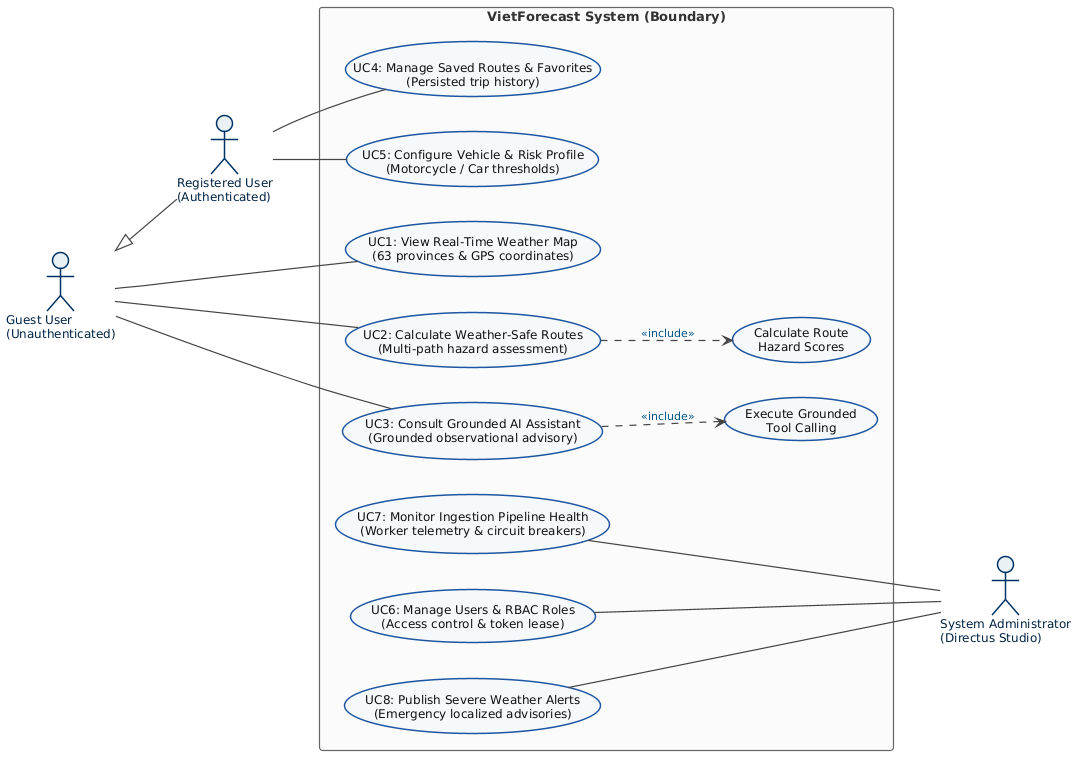
\includegraphics[width=0.95\textwidth]{figures/usecase.png}
\caption{Sơ đồ ca sử dụng tổng quan hệ thống VietForecast theo chuẩn UML 2.5.}
\label{fig:global_use_case_vi}
\end{figure}

\subsection{Bảng tổng hợp đặc tả các ca sử dụng}
Bảng~\ref{tab:use_case_summary_vi} tổng hợp danh mục toàn bộ tám ca sử dụng cốt lõi của hệ thống VietForecast cùng hai ca sử dụng phụ thuộc, phân loại theo nhóm tác nhân và mô tả mục tiêu nghiệp vụ tương ứng:

\begin{table}[H]
\centering
\small
\caption{Bảng tổng hợp đặc tả các ca sử dụng của hệ thống VietForecast.}
\label{tab:use_case_summary_vi}
\begin{tabularx}{\textwidth}{l p{3.4cm} p{2.6cm} X}
\toprule
\textbf{Mã} & \textbf{Tên ca sử dụng} & \textbf{Tác nhân} & \textbf{Mục tiêu và luồng xử lý chính} \\
\midrule
UC1 & Tra cứu bản đồ thời tiết & Guest User, Registered User & Hiển thị các lớp phủ thời tiết thời gian thực tại 63 tỉnh thành hoặc tọa độ định vị GPS. \\
\midrule
UC2 & Tính toán lộ trình an toàn & Guest User, Registered User & Khai phá ba lộ trình thay thế, tính toán ma trận điểm rủi ro và xếp hạng tuyến an toàn thời tiết nhất. Bao gồm ca sử dụng phụ thuộc tính điểm rủi ro. \\
\midrule
UC3 & Trợ lý đàm thoại AI & Guest User, Registered User & Hỗ trợ hỏi đáp tự nhiên bằng tiếng Việt; tự động kích hoạt gọi hàm kiểm chứng dữ liệu trạm quan trắc để ngăn chặn ảo giác thông tin. \\
\midrule
UC4 & Quản lý lộ trình ưa thích & Registered User & Lưu trữ lịch sử di chuyển, danh bạ điểm đến quen thuộc và cấu hình tuyến đường ưu tiên vào cơ sở dữ liệu. \\
\midrule
UC5 & Thiết lập cấu hình rủi ro & Registered User & Tùy biến loại phương tiện (xe máy, ô tô) và cấu hình các trọng số nhạy cảm cá nhân cho các yếu tố khí tượng. \\
\midrule
UC6 & Quản lý người dùng & System Administrator & Quản trị danh sách tài khoản, giám sát phân quyền RBAC và kiểm soát phiên đăng nhập thông qua Directus Studio. \\
\midrule
UC7 & Giám sát đường ống dữ liệu & System Administrator & Theo dõi nhịp tim của worker thu thập dữ liệu, giám sát trạng thái circuit breaker và kiểm tra tỷ lệ làm mới cache. \\
\midrule
UC8 & Phát hành cảnh báo khẩn & System Administrator & Soạn thảo, phê duyệt và phát sóng thông điệp cảnh báo thời tiết cực đoan tới người dùng trong khu vực ảnh hưởng. \\
\bottomrule
\end{tabularx}
\end{table}

\subsection{Đặc tả chi tiết các ca sử dụng cốt lõi}
Để làm rõ yêu cầu nghiệp vụ và hành vi tương tác của từng chức năng, chi tiết đặc tả luồng xử lý của các ca sử dụng được trình bày như sau:

\subsubsection{Ca sử dụng UC1: Tra cứu bản đồ thời tiết thời gian thực}
\begin{itemize}
    \item Tác nhân: Khách vãng lai (Guest User), Người dùng đã xác thực (Registered User).
    \item Tiền điều kiện: Thiết bị có kết nối Internet, dịch vụ API Gateway và giao diện bản đồ MapLibre GL sẵn sàng.
    \item Hậu điều kiện: Bản đồ hiển thị chính xác các lớp dữ liệu khí tượng (nhiệt độ, mưa, gió, tầm nhìn) tại địa điểm lựa chọn.
    \item Luồng sự kiện chính:
    \begin{enumerate}
        \item Người dùng truy cập trang chủ hệ thống hoặc nhấn nút định vị vị trí hiện tại qua GPS.
        \item Trình duyệt gửi yêu cầu truy vấn dữ liệu không gian đến API Gateway.
        \item Hệ thống kiểm tra dữ liệu trong bộ đệm Redis; nếu bộ đệm hợp lệ, trả về tức thì; nếu hết hạn, truy vấn trạm quan trắc gần nhất từ cơ sở dữ liệu PostgreSQL/PostGIS.
        \item Giao diện hiển thị các chỉ số thời tiết chi tiết kèm biểu đồ nhiệt màu trực quan trên nền bản đồ số.
    \end{enumerate}
    \item Luồng ngoại lệ: Nếu người dùng từ chối cấp quyền truy cập GPS, hệ thống mặc định chọn vị trí trung tâm Thủ đô Hà Nội và thông báo cho người dùng.
\end{itemize}

\subsubsection{Ca sử dụng UC2: Tính toán lộ trình an toàn thời tiết}
\begin{itemize}
    \item Tác nhân: Khách vãng lai (Guest User), Người dùng đã xác thực (Registered User).
    \item Quan hệ phụ thuộc: Bao gồm ($\ll$include$\gg$) ca sử dụng tính toán điểm rủi ro thời tiết (Calculate Route Hazard Scores).
    \item Tiền điều kiện: Người dùng nhập điểm xuất phát và điểm đích hợp lệ trong phạm vi lãnh thổ Việt Nam.
    \item Hậu điều kiện: Hệ thống trả về danh sách ba tuyến đường kèm theo điểm rủi ro tổng hợp và cảnh báo thời tiết dọc tuyến.
    \item Luồng sự kiện chính:
    \begin{enumerate}
        \item Người dùng nhập điểm bắt đầu, điểm kết thúc và lựa chọn phương tiện di chuyển (xe máy hoặc ô tô).
        \item Hệ thống gọi dịch vụ OSRM để trích xuất ba phương án lộ trình khả thi (Nhanh nhất, Ngắn nhất, Thay thế).
        \item Hệ thống phân đoạn từng lộ trình thành chuỗi các checkpoint không gian cách đều từ 5 đến 10 km.
        \item Kích hoạt ca sử dụng phụ thuộc tính điểm rủi ro: nội suy thời gian đến dự kiến (ETA) tại từng checkpoint, truy vấn dữ liệu dự báo thời tiết tương ứng và tính toán điểm rủi ro theo sáu chiều nguy cơ.
        \item Hệ thống tổng hợp điểm rủi ro, phân loại tuyến an toàn nhất (Safer Route) và hiển thị trực quan các đoạn nguy hiểm bằng dải màu cảnh báo trên bản đồ.
    \end{enumerate}
    \item Luồng ngoại lệ: Nếu dịch vụ OSRM ngoại vi gặp sự cố hoặc vượt thời gian chờ, hệ thống kích hoạt cơ chế retry; nếu vẫn thất bại, hiển thị thông báo lỗi mạng cho người dùng.
\end{itemize}

\subsubsection{Ca sử dụng UC3: Trợ lý đàm thoại AI có kiểm chứng}
\begin{itemize}
    \item Tác nhân: Khách vãng lai (Guest User), Người dùng đã xác thực (Registered User).
    \item Quan hệ phụ thuộc: Bao gồm ($\ll$include$\gg$) ca sử dụng gọi hàm kiểm chứng dữ liệu trạm quan trắc (Execute Grounded Tool Calling).
    \item Tiền điều kiện: Người dùng gửi câu hỏi liên quan đến thời tiết hoặc hành trình di chuyển vào khung trò chuyện.
    \item Hậu điều kiện: Trợ lý ảo phản hồi câu trả lời tự nhiên bằng tiếng Việt, dựa trên số liệu thực tế được kiểm chứng.
    \item Luồng sự kiện chính:
    \begin{enumerate}
        \item Người dùng nhập câu hỏi bằng ngôn ngữ tự nhiên về tình hình thời tiết hoặc cung đường di chuyển.
        \item API Gateway chuyển tiếp ngữ cảnh đàm thoại đến mô hình Google Gemini 1.5 Flash.
        \item Mô hình phát hiện ý định truy vấn khí tượng và phát sinh lệnh gọi hàm (function calling) với tham số tọa độ và địa danh cụ thể.
        \item Kích hoạt ca sử dụng phụ thuộc gọi hàm: backend thực thi truy vấn dữ liệu quan trắc thực tế của trạm khí tượng tương ứng và gửi kết quả có cấu trúc trở lại cho mô hình.
        \item Mô hình tổng hợp phản hồi đàm thoại súc tích, chính xác dựa trên số liệu đã kiểm chứng, hoàn toàn ngăn chặn hiện tượng ảo giác.
    \end{enumerate}
    \item Luồng ngoại lệ: Nếu địa danh người dùng hỏi không xác định được tọa độ, mô hình đưa ra câu hỏi làm rõ để người dùng cung cấp thêm thông tin vị trí.
\end{itemize}

\subsubsection{Ca sử dụng UC4: Quản lý lộ trình và địa điểm ưa thích}
\begin{itemize}
    \item Tác nhân: Người dùng đã xác thực (Registered User).
    \item Tiền điều kiện: Người dùng đã đăng nhập vào hệ thống với phiên làm việc hợp lệ.
    \item Hậu điều kiện: Thông tin lộ trình hoặc địa chỉ yêu thích được lưu trữ thành công vào hồ sơ cá nhân.
    \item Luồng sự kiện chính:
    \begin{enumerate}
        \item Người dùng nhấn nút lưu lộ trình vừa tìm kiếm hoặc thêm địa điểm quen thuộc vào danh bạ cá nhân.
        \item Ứng dụng gửi yêu cầu lưu trữ dữ liệu kèm theo cookie phiên bảo mật HttpOnly tới API Gateway.
        \item API Gateway xác thực tính hợp lệ của phiên qua Directus và ghi nhận dữ liệu vào bảng cơ sở dữ liệu PostgreSQL.
        \item Danh sách các hành trình đã lưu được cập nhật tức thì trên giao diện quản lý chuyến đi của người dùng.
    \end{enumerate}
    \item Luồng ngoại lệ: Nếu phiên làm việc của người dùng đã hết hạn, hệ thống thông báo yêu cầu đăng nhập lại mà không làm mất dữ liệu lộ trình đang mở.
\end{itemize}

\subsubsection{Ca sử dụng UC5: Thiết lập cấu hình phương tiện và ngưỡng nhạy cảm rủi ro}
\begin{itemize}
    \item Tác nhân: Người dùng đã xác thực (Registered User).
    \item Tiền điều kiện: Người dùng đã đăng nhập vào tài khoản cá nhân.
    \item Hậu điều kiện: Bộ tham số trọng số rủi ro cá nhân hóa được cập nhật và áp dụng cho các lần tìm kiếm lộ trình tiếp theo.
    \item Luồng sự kiện chính:
    \begin{enumerate}
        \item Người dùng truy cập trang cài đặt cấu hình an toàn di chuyển.
        \item Lựa chọn loại phương tiện mặc định (xe máy, ô tô) và tinh chỉnh các thanh trượt ngưỡng nhạy cảm với lượng mưa, vận tốc gió giật hoặc khoảng cách tầm nhìn.
        \item Người dùng nhấn xác nhận lưu cấu hình.
        \item Hệ thống cập nhật các trọng số vào bảng thuộc tính người dùng; các thuật toán tính điểm lộ trình sau đó sẽ tự động áp dụng ma trận trọng số này.
    \end{enumerate}
    \item Luồng ngoại lệ: Nếu người dùng nhập giá trị tham số nằm ngoài khoảng quy định, hệ thống từ chối cập nhật và hiển thị hướng dẫn nhập liệu hợp lệ.
\end{itemize}

\subsubsection{Ca sử dụng UC6: Quản lý người dùng và phân quyền RBAC}
\begin{itemize}
    \item Tác nhân: Quản trị viên hệ thống (System Administrator).
    \item Tiền điều kiện: Quản trị viên đăng nhập thành công vào giao diện Directus Admin Studio với quyền quản trị tối cao.
    \item Hậu điều kiện: Thông tin người dùng, vai trò hoặc quyền truy cập được cập nhật chính xác trong hệ thống.
    \item Luồng sự kiện chính:
    \begin{enumerate}
        \item Quản trị viên điều hướng đến mục quản lý người dùng trên giao diện quản trị Directus.
        \item Thực hiện các thao tác: duyệt danh sách tài khoản, kích hoạt, tạm khóa người dùng, hoặc gán vai trò quyền hạn (Role-Based Access Control).
        \item Hệ thống ghi nhận toàn bộ lịch sử thao tác vào nhật ký kiểm toán (audit log) để đảm bảo tính minh bạch và an toàn thông tin.
    \end{enumerate}
    \item Luồng ngoại lệ: Hệ thống ngăn chặn hành vi tự xóa tài khoản hoặc tự hạ quyền quản trị của chính tài khoản đang đăng nhập để tránh mất quyền điều hành.
\end{itemize}

\subsubsection{Ca sử dụng UC7: Giám sát đường ống thu thập dữ liệu}
\begin{itemize}
    \item Tác nhân: Quản trị viên hệ thống (System Administrator).
    \item Tiền điều kiện: Quản trị viên truy cập trang tổng quan giám sát hệ thống.
    \item Hậu điều kiện: Trạng thái vận hành của các dịch vụ ngầm và đường ống dữ liệu được cập nhật đầy đủ.
    \item Luồng sự kiện chính:
    \begin{enumerate}
        \item Quản trị viên kiểm tra bảng điều khiển hiển thị trạng thái của tiến trình Integration Worker.
        \item Hệ thống cung cấp thông tin nhịp tim (heartbeat), thời điểm cập nhật dữ liệu gần nhất, trạng thái circuit breaker và tỷ lệ thành công của các yêu cầu gửi đến nhà cung cấp thời tiết ngoại vi.
        \item Nếu phát hiện dấu hiệu bất thường (như dữ liệu quan trắc trễ quá 60 phút hoặc lỗi API liên tiếp), hệ thống hiển thị cảnh báo mức đỏ.
    \end{enumerate}
    \item Luồng ngoại lệ: Khi đường ống chính gặp sự cố, hệ thống cho phép quản trị viên kích hoạt chế độ tải dữ liệu thủ công từ nguồn dự phòng.
\end{itemize}

\subsubsection{Ca sử dụng UC8: Phát hành bản tin cảnh báo thời tiết khẩn cấp}
\begin{itemize}
    \item Tác nhân: Quản trị viên hệ thống (System Administrator).
    \item Tiền điều kiện: Quản trị viên ghi nhận thông tin thiên tai, bão lũ hoặc hiện tượng thời tiết nguy hiểm cần thông báo khẩn cấp.
    \item Hậu điều kiện: Bản tin cảnh báo được lưu vào cơ sở dữ liệu và hiển thị nổi bật trên bản đồ số của tất cả người dùng trong vùng ảnh hưởng.
    \item Luồng sự kiện chính:
    \begin{enumerate}
        \item Quản trị viên mở biểu mẫu tạo thông báo khẩn cấp trên giao diện quản trị.
        \item Nhập nội dung cảnh báo, chọn mức độ rủi ro (vàng, cam, đỏ) và xác định phạm vi địa lý bị ảnh hưởng (danh sách tỉnh thành hoặc đa giác tọa độ).
        \item Quản trị viên nhấn nút phê duyệt phát hành bản tin.
        \item Hệ thống lưu trữ bản tin và đồng bộ trạng thái để kích hoạt biểu tượng cảnh báo tức thời trên giao diện ứng dụng của người dùng.
    \end{enumerate}
    \item Luồng ngoại lệ: Nếu quản trị viên chưa chọn phạm vi địa lý hoặc nội dung cảnh báo còn để trống, hệ thống yêu cầu hoàn thiện đầy đủ các trường thông tin bắt buộc trước khi phát sóng.
\end{itemize}

\section{Kiến trúc hệ thống mức khái niệm}
Để hiện thực hóa các yêu cầu chức năng và phi chức năng đã đề ra, đồng thời bảo đảm tính toàn vẹn và độ tin cậy của dịch vụ, hệ thống VietForecast được mô hình hóa theo sơ đồ ngữ cảnh C4 (C4 Model Level 1 -- System Context) như thể hiện trong Hình~\ref{fig:conceptual_overview_vi}. Mô hình phân định rõ ranh giới hệ thống, các nhóm tác nhân tương tác và các dịch vụ đám mây ngoại vi:
\begin{itemize}
    \item Nhóm tác nhân người dùng (Platform Users): Bao gồm người tham gia giao thông (Commuter / Traveler) truy cập hệ thống qua ứng dụng web để tra cứu thời tiết, tìm kiếm lộ trình an toàn và tương tác với trợ lý AI; cùng quản trị viên hệ thống (System Administrator) thực hiện cấu hình vận hành, giám sát đường ống dữ liệu và phát hành các bản tin cảnh báo khẩn cấp qua giao diện Directus Admin Studio.
    \item Nền tảng trung tâm VietForecast (Core Software System): Là thành phần cốt lõi của giải pháp, chịu trách nhiệm tiếp nhận và xử lý các yêu cầu từ phía người dùng thông qua API Gateway hiệu năng cao. Hệ thống tự động điều phối tiến trình thu thập và chuẩn hóa dữ liệu từ các trạm khí tượng, vận hành động cơ đánh giá rủi ro đa chiều, thực thi thuật toán tìm kiếm lộ trình an toàn thời tiết và cung cấp giao diện hội thoại thông minh có kiểm chứng dữ liệu thực tế.
    \item Các dịch vụ đám mây ngoại vi (External Cloud Services): Bao gồm dịch vụ WeatherAPI cung cấp dữ liệu quan trắc thời gian thực và dự báo số trị chuẩn WMO; dịch vụ OSRM kết hợp bản đồ OpenStreetMap \cite{haklay2008openstreetmap} cung cấp đồ thị mạng lưới đường bộ và thuật toán tìm đường cơ sở; cùng mô hình ngôn ngữ lớn Google Gemini 1.5 Flash đóng vai trò khối suy luận ngôn ngữ tự nhiên được kiểm soát chặt chẽ thông qua giao thức gọi hàm nội bộ.
\end{itemize}

\begin{figure}[H]
\centering
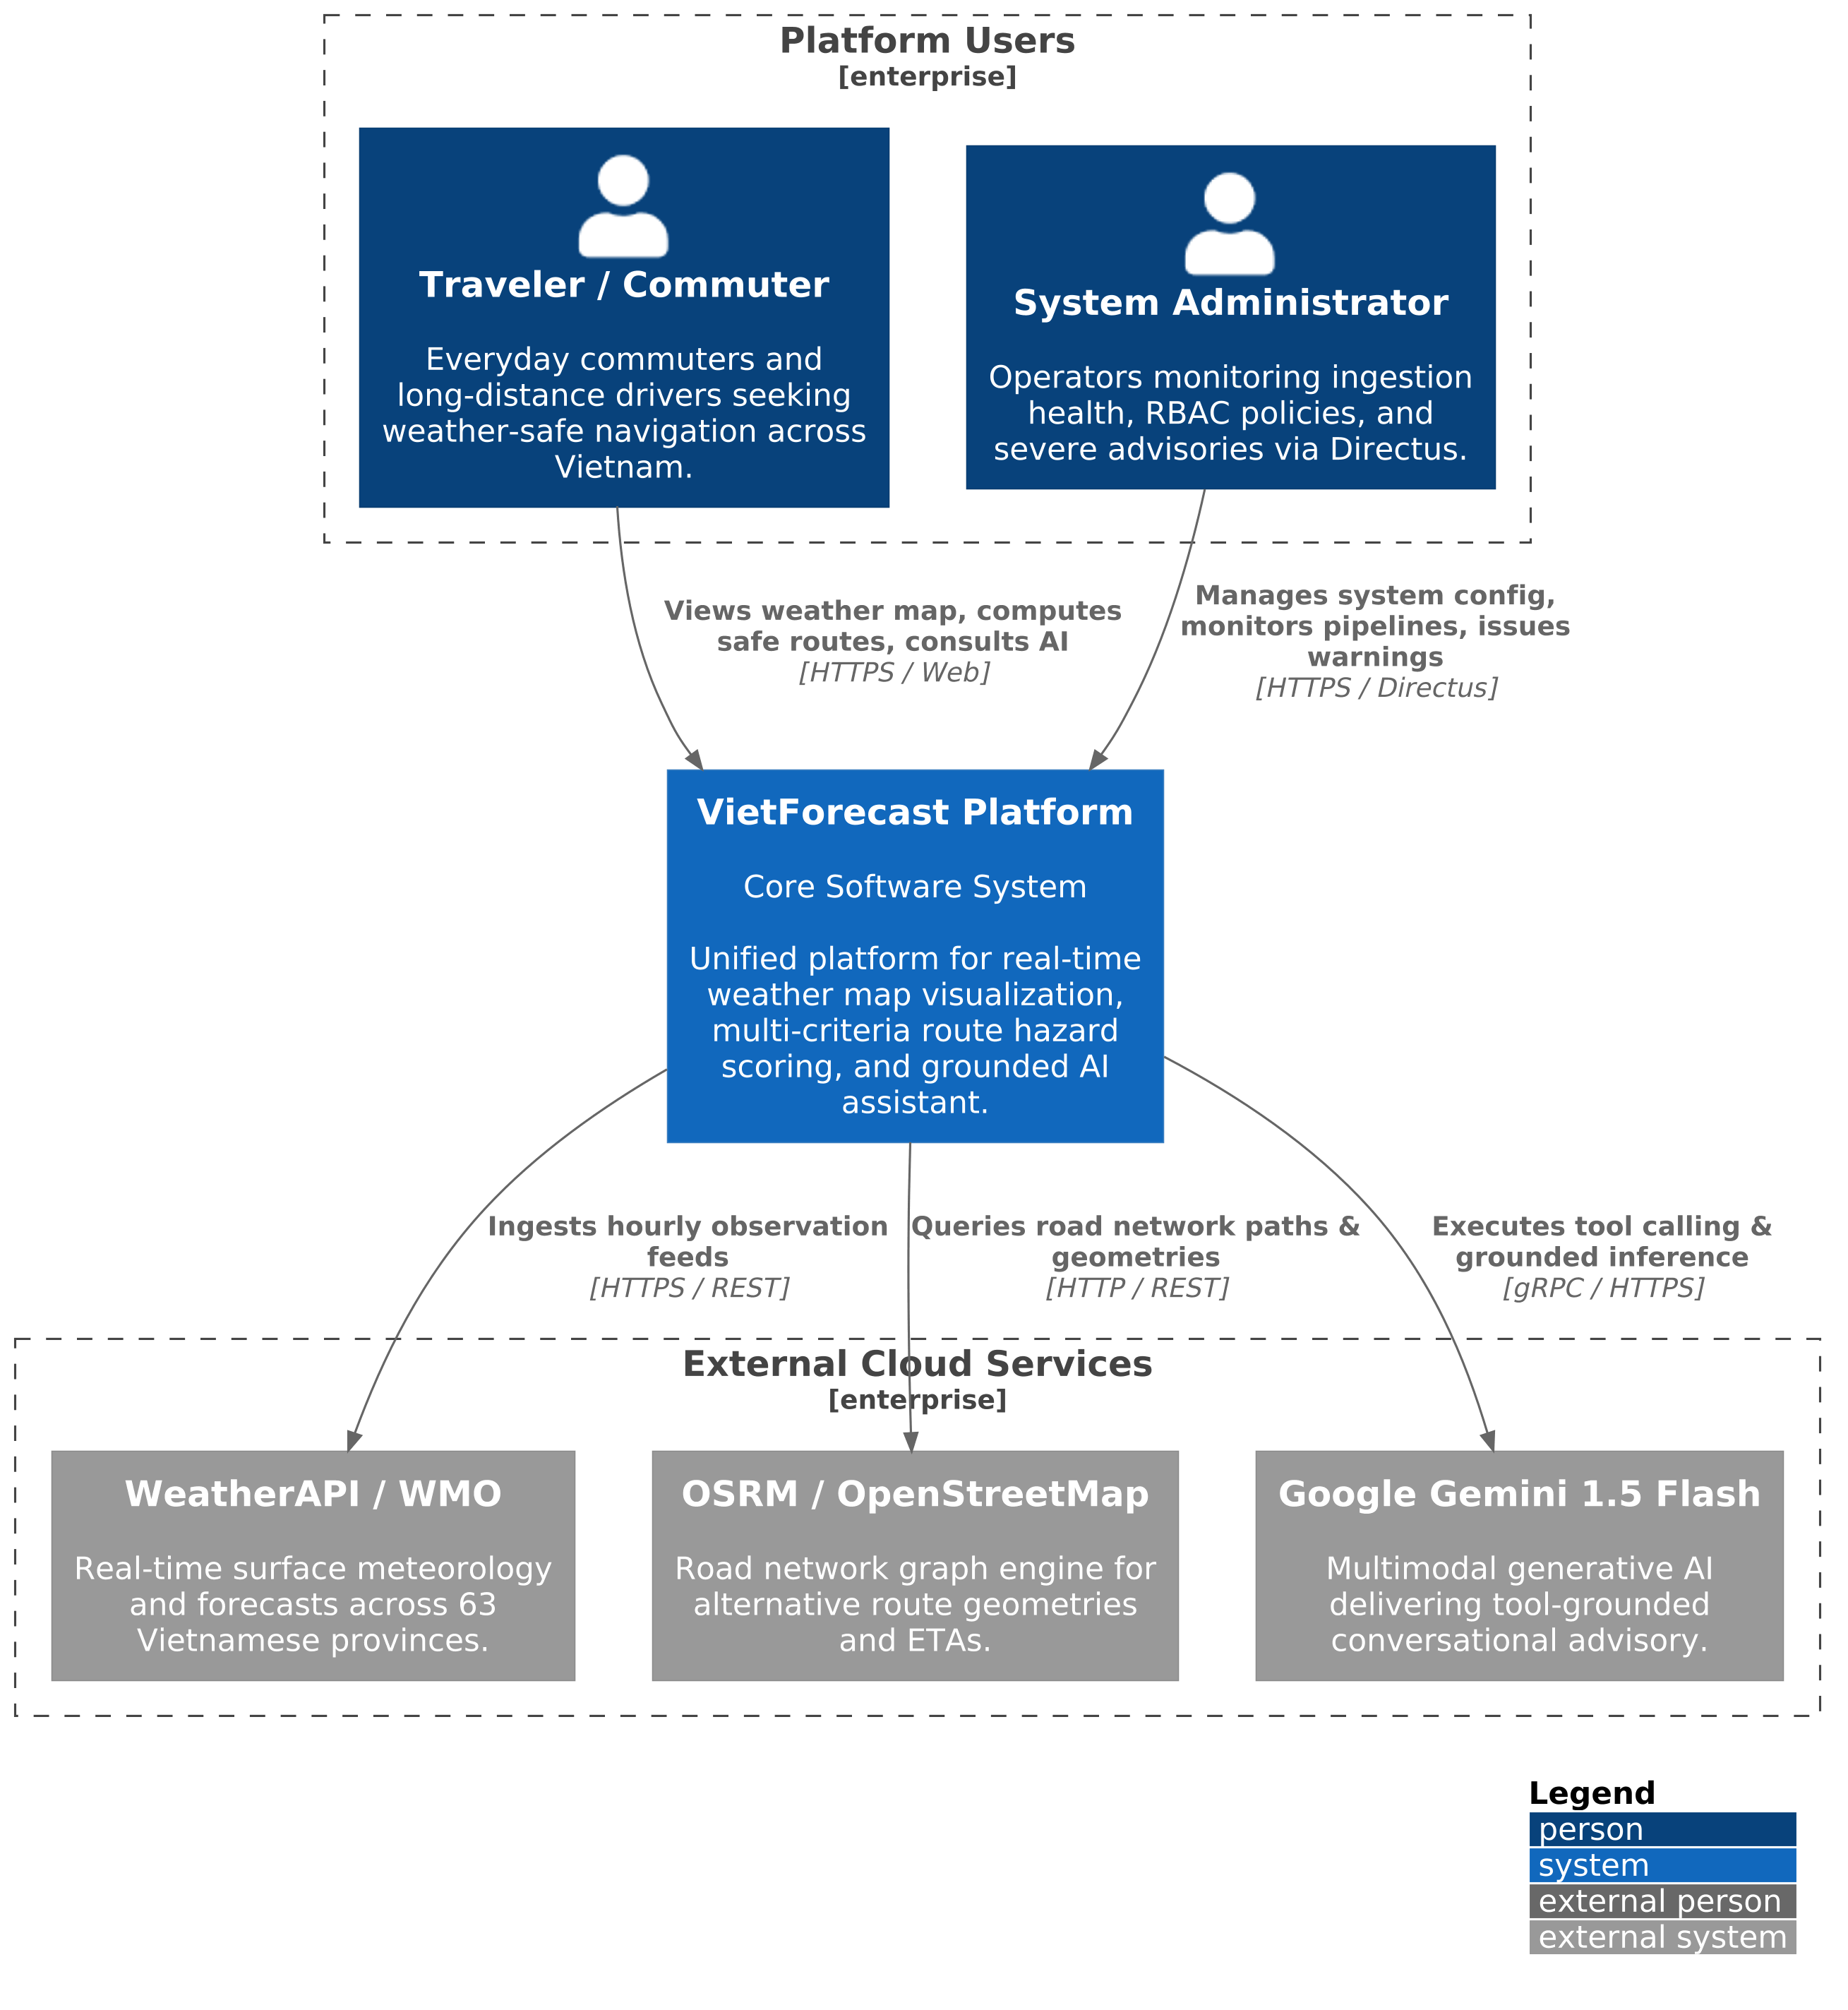
\includegraphics[width=0.92\textwidth]{figures/c4_context.png}
\caption{Sơ đồ ngữ cảnh hệ thống VietForecast theo mô hình C4 (C4 Context Diagram).}
\label{fig:conceptual_overview_vi}
\end{figure}



\chapter{Cơ sở lý thuyết và Công nghệ nền tảng}
\label{ch:theory}

Chương này trình bày toàn diện các nền tảng lý thuyết khoa học, mô hình tính toán định lượng và kiến trúc công nghệ nền tảng được nghiên cứu và ứng dụng trong hệ sinh thái VietForecast. Nội dung trọng tâm đi từ nguyên lý biểu diễn và xử lý dữ liệu địa lý không gian trong GIS, quy chuẩn đo lường khí tượng bề mặt theo tiêu chuẩn của Tổ chức Khí tượng Thế giới (WMO), thuật toán rời rạc hóa và định lượng rủi ro đa chiều trên hành lang giao thông, cho đến kỹ thuật đối soát dữ liệu thực (Tool Grounding) loại trừ hiện tượng ảo tưởng của mô hình ngôn ngữ lớn và các phân tích chuyên sâu về ngăn xếp công nghệ phân tán được lựa chọn.

\section{Dữ liệu không gian địa lý và Hệ thống thông tin địa lý (GIS)}

Hệ thống thông tin địa lý (Geographic Information System -- GIS) đóng vai trò nền tảng trong toàn bộ chu trình xử lý của VietForecast, từ tiếp nhận tọa độ, chuyển đổi hệ quy chiếu, biểu diễn topo mạng lưới giao thông đường bộ đến thực thi các phép phân tích lân cận không gian giữa phương tiện di chuyển và các trạm quan trắc khí tượng bề mặt.

\subsection{Hệ quy chiếu WGS84 và Đặc tả GeoJSON RFC 7946}

Để định vị chính xác vị trí tuyệt đối của các đối tượng địa lý trên bề mặt Trái Đất, hệ thống sử dụng Hệ quy chiếu trắc địa thế giới năm 1984 (World Geodetic System 1984 -- WGS84), được chuẩn hóa quốc tế dưới mã nhận dạng EPSG:4326. Mô hình toán học của WGS84 xấp xỉ bề mặt geoid thực tế của Trái Đất thông qua một hình elipxoit xoay (oblate ellipsoid of revolution) được xác định bởi hai hằng số hình học cơ bản:
\begin{itemize}
    \item[-] Bán trục lớn xích đạo: $a = 6.378.137\text{ m}$.
    \item[-] Độ dẹt hình học: $f = \frac{a - b}{a} = \frac{1}{298{,}257223563}$.
\end{itemize}
Từ hai tham số này, bán trục nhỏ cực $b$ được xác định xấp xỉ:
\begin{equation}
\label{eq:minor_axis_vi}
b = a(1 - f) \approx 6.356.752{,}3142\text{ m}
\end{equation}
Vị trí của một thực thể địa lý bất kỳ $P$ trên mặt cầu elipxoit được định danh duy nhất bởi cặp tọa độ trắc địa $(\phi, \lambda)$, trong đó $\phi \in [-90^\circ, +90^\circ]$ biểu thị vĩ độ và $\lambda \in [-180^\circ, +180^\circ]$ biểu thị kinh độ.

Trong tầng giao tiếp dịch vụ và truyền tải dữ liệu qua giao diện lập trình ứng dụng (API), định dạng GeoJSON theo đặc tả chuẩn RFC 7946 \cite{rfc7946} được áp dụng làm phương thức đóng gói tiêu chuẩn. GeoJSON sử dụng cấu trúc cú pháp JSON để mô tả các đối tượng không gian. Một điểm kỹ thuật tối quan trọng theo RFC 7946 là quy ước thứ tự tọa độ: kinh độ (easting) luôn được xếp trước vĩ độ (northing) theo cặp $[\lambda, \phi]$, hoàn toàn trái ngược với thói quen phát biểu thông thường $(latitude, longitude)$. Các kiểu hình học cơ bản được hệ thống khai thác bao gồm:
\begin{itemize}
    \item[-] Điểm (Point): Định danh vị trí trạm quan trắc khí tượng hoặc tọa độ tức thời của phương tiện giao thông, ví dụ $[105.8542, 21.0285]$ đại diện cho vị trí trạm đo tại khu vực Hà Nội.
    \item[-] Đa tuyến (LineString): Chuỗi liên tục các điểm nút không gian kết nối với nhau, mô tả quỹ đạo hình học của các cung đường quốc lộ, cao tốc hoặc lộ trình đề xuất cho phương tiện.
    \item[-] Vùng đa giác (Polygon và MultiPolygon): Xác định đường bao ranh giới hành chính của 63 tỉnh thành phố tại Việt Nam, cũng như diện bao phủ không gian của các vùng nhiễu động mây dông hoặc tâm áp thấp nhiệt đới.
    \item[-] Tập hợp đối tượng (FeatureCollection): Cấu trúc mảng chứa danh sách các đối tượng hình học độc lập (Features), cho phép gắn kèm các thuộc tính phi không gian (properties) như hệ số trơn trượt mặt đường, tốc độ gió tức thời và chỉ số cảnh báo rủi ro.
\end{itemize}

\subsection{Hệ quản trị dữ liệu không gian PostGIS và Cơ chế chỉ mục GiST}

Việc lưu trữ, quản lý và truy vấn hàng triệu đối tượng hình học với yêu cầu độ trễ dưới một giây đặt ra thách thức lớn đối với các hệ quản trị cơ sở dữ liệu quan hệ truyền thống. VietForecast triển khai PostGIS \cite{postgis2023} -- một module mở rộng không gian chạy trên nền tảng PostgreSQL 16. PostGIS bổ sung các kiểu dữ liệu không gian tuân thủ đặc tả Open Geospatial Consortium (OGC) bao gồm \texttt{geometry} (phép tính phẳng trong hệ tọa độ Descartes) và \texttt{geography} (phép tính cầu trắc địa trên mặt cong elipxoit thực tế).

Khi kích thước tập dữ liệu không gian tăng lên, việc quét tuần tự toàn bộ bảng dữ liệu (sequential scan) dẫn tới độ phức tạp thời gian $O(N)$, gây tắc nghẽn tài nguyên CPU nghiêm trọng khi có nhiều người dùng đồng thời yêu cầu phân tích hành trình. Để giải quyết triệt để vấn đề này, PostGIS cung cấp cấu trúc chỉ mục cây tìm kiếm tổng quát GiST (Generalized Search Tree) kế thừa nguyên lý cấu trúc cây R-Tree \cite{guttman1984}.

Chỉ mục GiST hoạt động bằng cách bao bọc mỗi đối tượng hình học phức tạp bằng một hộp chữ nhật bao tối thiểu (Bounding Box -- BBOX) có các cạnh song song với các trục tọa độ địa lý. Cây GiST được tổ chức theo cấu trúc phân cấp nhiều tầng: các nút lá lưu giữ BBOX của từng đối tượng riêng lẻ, còn các nút nhánh cha lưu giữ BBOX bao trùm toàn bộ các BBOX của các nút con trực thuộc. Khi tiếp nhận một câu truy vấn không gian, hệ thống kích hoạt quy trình lọc hai bước:
\begin{itemize}
    \item[-] Giai đoạn lọc thô (Rough Pass): Hộp BBOX của đối tượng truy vấn duyệt qua cây chỉ mục với độ phức tạp tiệm cận $O(\log N)$. Thuật toán loại bỏ lập tức đại đa số các đối tượng có hộp bao không giao cắt với vùng quan tâm mà không cần truy xuất tới dữ liệu hình học chi tiết.
    \item[-] Giai đoạn tính toán chính xác (Exact Pass): Các phép toán hình học hình cầu chi tiết chỉ được áp dụng trên tập hợp rất nhỏ các đối tượng còn lại đã vượt qua giai đoạn lọc thô, giúp tiết kiệm tối đa tài nguyên xử lý.
\end{itemize}

Trong quá trình phân tích tương quan giữa lộ trình và thời tiết, hệ thống khai thác các hàm không gian cốt lõi của PostGIS:
\begin{itemize}
    \item[-] \texttt{ST\_DWithin(geom1, geom2, distance)}: Xác định các trạm quan trắc nằm trong bán kính ảnh hưởng của cung đường thông qua việc khai thác trực tiếp chỉ mục GiST mà không cần tính khoảng cách từng đôi một trên toàn bảng.
    \item[-] \texttt{ST\_DistanceSphere(geom1, geom2)}: Tính khoảng cách cung tròn xấp xỉ giữa hai tọa độ địa lý trên mặt cầu chuẩn, giúp tối ưu hóa thời gian tính toán với sai số trắc địa không đáng kể ở quy mô khu vực.
    \item[-] \texttt{ST\_LineInterpolatePoint(line, fraction)}: Trích xuất tọa độ điểm nội suy tại vị trí tỷ lệ xác định dọc theo tuyến đường, cung cấp cơ sở toán học để thực hiện việc rời rạc hóa tuyến đường theo khoảng cách.
\end{itemize}

\subsection{Giải thuật rời rạc hóa và lấy mẫu hành lang di chuyển}

Một hành trình di chuyển liên tỉnh tại Việt Nam thường kéo dài từ hàng chục đến hàng trăm kilômét, đi qua nhiều địa hình phân hóa phức tạp như đồng bằng duyên hải, đèo dốc và cao nguyên. Dữ liệu khí tượng đo được tại điểm xuất phát vào thời điểm $t_0$ hoàn toàn không đại diện cho điều kiện thời tiết tại một con đèo cách xa 120~km mà phương tiện sẽ tiếp cận sau ba giờ lái xe. Do đó, hệ thống xây dựng giải thuật rời rạc hóa không gian kết hợp ước lượng thời gian tiếp cận thực tế dọc tuyến đường.

Khoảng cách trắc địa cung tròn giữa hai điểm tọa độ kế tiếp $(\phi_1, \lambda_1)$ và $(\phi_2, \lambda_2)$ được tính toán thông qua công thức Haversine:
\begin{equation}
\label{eq:haversine_vi}
d = 2R \cdot \arcsin \left( \sqrt{\sin^2\left(\frac{\Delta \phi}{2}\right) + \cos\phi_1 \cos\phi_2 \sin^2\left(\frac{\Delta \lambda}{2}\right)} \right)
\end{equation}
trong đó $R \approx 6.371\text{ km}$ là bán kính trung bình của Trái Đất, $\Delta \phi = \phi_2 - \phi_1$ và $\Delta \lambda = \lambda_2 - \lambda_1$ tính theo đơn vị radian.

Gọi $L$ là tổng chiều dài hành trình và $T$ là tổng thời gian lưu thông dự kiến được cung cấp bởi động cơ định tuyến đường bộ, vận tốc di chuyển trung bình danh định dọc hành lang được xác định bởi $\bar{v} = L / T$. Thuật toán tiến hành rời rạc hóa đối tượng LineString của tuyến đường thành một tập hợp hữu hạn các điểm kiểm tra khí tượng $\mathcal{P}_{\text{samples}} = \{p_0, p_1, p_2, \dots, p_K\}$ thỏa hiệp đồng thời hai giới hạn trên:
\begin{itemize}
    \item[-] Bước không gian tối đa: Khoảng cách giữa hai điểm mẫu liên tiếp không được vượt quá $\Delta s_{\max} = 5\text{ km}$.
    \item[-] Bước thời gian tối đa: Khoảng thời gian di chuyển dự kiến giữa hai điểm mẫu kế tiếp không được vượt quá $\Delta t_{\max} = 15\text{ phút}$.
\end{itemize}

Tại mỗi điểm kiểm tra $p_i$, mốc thời gian phương tiện dự kiến chạm mốc được ước lượng lũy kế:
\begin{equation}
\label{eq:arrival_time_vi}
t_i = t_0 + \sum_{j=1}^{i} \frac{d(p_{j-1}, p_j)}{\bar{v}}
\end{equation}
Sau đó, hệ thống thiết lập một vùng đệm không gian (buffer corridor) có bán kính ảnh hưởng $r_{\text{corridor}} = 15\text{ km}$ xung quanh điểm $p_i$. Nhờ vùng đệm này, câu truy vấn không gian sẽ nhanh chóng xác định được trạm quan trắc gần nhất hoặc lấy giá trị trường thời tiết dự báo tương ứng với mốc thời gian $t_i$ để gán vào điểm kiểm tra.

\section{Tiêu chuẩn khí tượng WMO và Mô hình định lượng rủi ro}

\subsection{Quy chuẩn quan trắc bề mặt WMO-No. 8 và Chuẩn hóa dữ liệu}

Dữ liệu khí tượng đầu vào của VietForecast được chuẩn hóa dựa trên tài liệu Hướng dẫn về Dụng cụ và Phương pháp Quan trắc số 8 (WMO-No. 8) do Tổ chức Khí tượng Thế giới ban hành \cite{wmo2021guidelines}. Năm đại lượng vật lý nòng cốt ảnh hưởng trực tiếp đến động lực học di chuyển, hệ số ma sát giữa lốp xe và mặt đường bao gồm:
\begin{itemize}
    \item[-] Cường độ lượng mưa tức thời ($I_{\text{rain}}$, tính bằng mm/h): Mưa lớn làm giảm ma sát tiếp xúc, tích tụ màng nước trên mặt đường dẫn đến hiện tượng trượt nước nguy hiểm (hydroplaning) làm phương tiện mất hoàn toàn lực phanh và lái.
    \item[-] Tốc độ gió duy trì ($v_{\text{wind}}$) và tốc độ gió giật ($v_{\text{gust}}$, tính bằng km/h): Gió giật ngang với vận tốc lớn tạo ra mô-men lật khí động học, đặc biệt nguy hiểm đối với xe hai bánh khi di chuyển qua cầu vượt biển hoặc các cung đường đèo lộng gió.
    \item[-] Tầm nhìn ngang mặt đất ($V_{\text{vis}}$, tính bằng mét): Sự suy giảm tầm nhìn do sương mù bức xạ, sương mù bình lưu hoặc mưa rào cường độ mạnh làm co hẹp cự ly quan sát an toàn và kéo dài thời gian phản ứng trước chướng ngại vật.
    \item[-] Nhiệt độ không khí bề mặt ($T_{\text{air}}$, tính bằng $^\circ$C): Nắng nóng cực đoan trên $39^\circ$C làm tăng áp suất lốp, dễ gây nổ lốp và suy nhược thể lực người lái; nhiệt độ rét đậm dưới $10^\circ$C kết hợp sương muối ở vùng núi cao gây hiện tượng đóng băng mặt đường.
    \item[-] Cảnh báo thiên tai cực đoan: Các bản tin chính thống về áp thấp nhiệt đới, bão biển Đông, lũ quét và sạt lở ta-luy đường bộ.
\end{itemize}

Trong tầng xử lý dữ liệu nền, các mã hiện tượng khí tượng từ nhà cung cấp ngoài được ánh xạ về một tập danh mục điều kiện chuẩn hóa nội bộ (gồm các trạng thái như \texttt{clear}, \texttt{cloudy}, \texttt{fog}, \texttt{rain} và \texttt{thunderstorm}). Mỗi gói dữ liệu chuẩn hóa đều được tính toán mã băm SHA-256 để đảm bảo tính toàn vẹn và hỗ trợ cơ chế lưu đệm khử trùng lặp dữ liệu.

\subsection{Vòng đời độ tươi mới dữ liệu và Nguyên tắc vận hành an toàn (Fail-Safe)}

Hiện tượng khí quyển luôn biến thiên liên tục và phi tuyến tính. Một số liệu quan trắc dù đạt độ chính xác cao tại thời điểm đo cũng sẽ suy giảm nhanh chóng giá trị thực tế sau một khoảng thời gian nhất định. Nhằm ngăn ngừa rủi ro đưa ra chỉ dẫn dẫn đường sai lệch do dữ liệu cũ, VietForecast thiết lập mô hình vòng đời kiểm soát độ tươi mới của dữ liệu (Data Freshness Lifecycle theo quyết định RISK-006) gồm ba trạng thái:
\begin{itemize}
    \item[-] Tươi mới (Fresh): Độ tuổi dữ liệu $\tau = t_{\text{hiện tại}} - t_{\text{quan trắc}} \le 60\text{ phút}$ đối với quan trắc tức thời và không quá 24 giờ đối với dữ liệu dự báo. Dữ liệu trong khoảng này được phép đưa thẳng vào thuật toán đánh giá rủi ro.
    \item[-] Đang cũ (Aging): $60\text{ phút} < \tau \le 180\text{ phút}$. Dữ liệu vẫn được sử dụng nhưng hệ thống bắt buộc gắn kèm nhãn cảnh báo suy giảm độ tin cậy để người dùng tự nhận định.
    \item[-] Hết hạn (Stale): $\tau > 180\text{ phút}$ hoặc mất tín hiệu kết nối từ trạm đo.
\end{itemize}

Hệ thống quán triệt nguyên tắc an toàn tuyệt đối (Fail-Safe Principle): khi dữ liệu rơi vào trạng thái Stale hoặc không có sẵn dữ liệu, hệ thống kiên quyết từ chối mọi phép suy diễn phỏng đoán và tự động đưa mức độ rủi ro tại vị trí đó về trạng thái Không xác định (Unknown -- mã điểm 0, hiển thị màu xám trung tính \#9CA3AF). Nguyên tắc này bảo đảm hệ sinh thái không bao giờ ngộ nhận một cung đường thiếu dữ liệu là an toàn, đặt sự an toàn sinh mạng của người tham gia giao thông lên hàng đầu.

\subsection{Ma trận rủi ro đa chiều và Giải thuật tổng hợp rủi ro hành lang}

Nhằm chuyển đổi các biến số vật lý rời rạc thành chỉ số cảnh báo trực quan phục vụ người dùng, hệ thống xây dựng mô hình ma trận đánh giá rủi ro đa chiều. Không gian trạng thái rủi ro được chia thành 4 cấp độ phân biệt (quyết định RISK-001): Thấp (Low -- điểm 1, màu xanh lá), Chú ý (Caution -- điểm 2, màu vàng), Nguy hiểm (High -- điểm 3, màu cam đậm) và Không xác định (Unknown -- điểm 0, màu xám).

Mỗi điểm mẫu $p_i$ trên lộ trình được đánh giá độc lập trên 6 chiều rủi ro thành phần (quyết định RISK-002): mưa ($R_{\text{rain}}$), gió ($R_{\text{wind}}$), nhiệt độ ($R_{\text{temp}}$), tầm nhìn ($R_{\text{vis}}$), dông sét ($R_{\text{storm}}$) và cảnh báo thiên tai chính thức ($R_{\text{alert}}$). Bảng~\ref{tab:risk_matrix_thresholds_vi} chi tiết hóa các ngưỡng giá trị phân định rủi ro tiêu chuẩn được áp dụng trong hệ thống.

\begin{table}[H]
\centering
\caption{Bảng ngưỡng phân định rủi ro khí tượng theo tiêu chuẩn WMO trong VietForecast.}
\label{tab:risk_matrix_thresholds_vi}
\footnotesize
\renewcommand{\arraystretch}{0.92}
\begin{tabularx}{\textwidth}{>{\raggedright\arraybackslash}p{4.2cm} *{3}{>{\centering\arraybackslash}X}}
\toprule
Tham số khí tượng đo lường & Cấp 1 (Thấp) & Cấp 2 (Chú ý) & Cấp 3 (Nguy hiểm) \\
\midrule
Cường độ mưa ($I_{\text{rain}}$) & $< 5\text{ mm/h}$ & $5 - 20\text{ mm/h}$ & $> 20\text{ mm/h}$ \\
Gió giật cực đại ($v_{\text{gust}}$) & $< 30\text{ km/h}$ & $30 - 50\text{ km/h}$ & $> 50\text{ km/h}$ \\
Tầm nhìn xa ngang ($V_{\text{vis}}$) & $> 2.000\text{ m}$ & $500 - 2.000\text{ m}$ & $< 500\text{ m}$ \\
Nhiệt độ cực đoan ($T_{\text{air}}$) & $18 - 35^\circ$C & $10 - 18^\circ$C hoặc $35 - 39^\circ$C & $< 10^\circ$C hoặc $> 39^\circ$C \\
Hoạt động dông sét / lốc xoáy & Không xuất hiện & Mưa dông nhiệt cục bộ & Dông sét dữ dội / ngập lụt diện rộng \\
\bottomrule
\end{tabularx}
\end{table}

Cấp độ rủi ro tổng hợp tại mỗi điểm kiểm tra $p_i$ tuân thủ nguyên tắc bao trùm rủi ro nghiêm trọng nhất (Max-Severity Rule theo quyết định RISK-005):
\begin{equation}
\label{eq:point_risk}
S(p_i) = \max \left( R_{\text{rain}}(p_i), R_{\text{wind}}(p_i), R_{\text{temp}}(p_i), R_{\text{vis}}(p_i), R_{\text{storm}}(p_i), R_{\text{alert}}(p_i) \right)
\end{equation}

Từ tập hợp các điểm mẫu, chỉ số rủi ro đại diện cho toàn bộ cung đường $S_{\text{route}}$ được xác định theo điểm số cao nhất xuất hiện trên lộ trình:
\begin{equation}
\label{eq:route_risk_max}
S_{\text{route}} = \max_{i=1,\dots,K} S(p_i)
\end{equation}
Bên cạnh giá trị cực đại, hệ thống tính toán thêm điểm rủi ro trung bình có trọng số theo chiều dài phân đoạn:
\begin{equation}
\label{eq:route_risk_avg}
\bar{S}_{\text{route}} = \frac{\sum_{i=1}^{K-1} d(p_{i-1}, p_i) \cdot \frac{S(p_{i-1}) + S(p_i)}{2}}{\sum_{i=1}^{K-1} d(p_{i-1}, p_i)}
\end{equation}
Nếu trên hành trình tồn tại bất kỳ phân đoạn nào đạt mức $S(p_i) = 3$ (chẳng hạn một đoạn đèo sạt lở hoặc ngập nước sâu), toàn bộ tuyến đường sẽ được gắn mác cảnh báo Nguy hiểm để người điều khiển phương tiện kịp thời đổi sang hướng tuyến khác.

\subsection{Phân hóa đặc thù phương tiện và Hàm tối ưu lộ trình đa mục tiêu}

Giao thông Việt Nam mang đặc thù rất riêng với hơn 70 triệu xe máy đang lưu hành, chiếm trên 85\% tổng phương tiện cá nhân. Người đi xe máy không có cabin che chắn cơ học, chịu tác động trực tiếp của gió tạt ngang, hạt mưa táp vào mặt làm mờ kính chắn gió và bề mặt lốp nhỏ dễ mất lực bám khi phanh gấp. Do đó, hệ thống tích hợp cơ chế hiệu chỉnh ngưỡng nhạy cảm rủi ro theo loại phương tiện (quyết định ROUTE-001):
\begin{itemize}
    \item[-] Đối với xe máy (\texttt{motorcycle}): Ngưỡng kích hoạt rủi ro của gió giật ($v_{\text{gust}}$) và tầm nhìn hạn chế ($V_{\text{vis}}$) được siết chặt hơn 30\% so với ô tô. Ví dụ, gió giật trên $35\text{ km/h}$ đã bị xếp vào cấp độ Chú ý đối với người đi xe máy.
    \item[-] Đối với ô tô con (\texttt{car}): Áp dụng các ngưỡng tiêu chuẩn của WMO, tận dụng lợi thế ổn định trọng tâm xe và hệ thống gạt mưa kính chắn gió.
\end{itemize}

Khi người dùng tìm kiếm đường đi, hệ thống tính toán đồng thời 3 phương án lộ trình thay thế (quyết định ROUTE-003): phương án nhanh nhất (Fastest), ngắn nhất (Shortest) và an toàn thời tiết nhất (Weather-safer). Để hỗ trợ người dùng ra quyết định, hệ thống tổng hợp một hàm chấm điểm cân bằng đa mục tiêu (quyết định ROUTE-004):
\begin{equation}
\label{eq:balanced_route_score}
Score_{\text{balanced}} = w_{\text{risk}} \cdot \hat{S}_{\text{route}} + w_{\text{time}} \cdot \hat{T} + w_{\text{dist}} \cdot \hat{D}
\end{equation}
trong đó $\hat{S}_{\text{route}}, \hat{T}, \hat{D} \in [0, 1]$ là các giá trị chuẩn hóa của chỉ số rủi ro thời tiết, thời gian lưu thông và quãng đường di chuyển. Bộ trọng số mặc định được hiệu chỉnh linh hoạt qua bảng cấu hình Directus với $w_{\text{risk}} = 0{,}5$, $w_{\text{time}} = 0{,}3$, $w_{\text{dist}} = 0{,}2$, thể hiện rõ định hướng ưu tiên an toàn thời tiết của nền tảng.

\section{Mô hình ngôn ngữ lớn và Kỹ thuật Function Calling có kiểm chứng}

\subsection{Hạn chế cố hữu của LLM tự hồi quy trong bài toán an toàn giao thông}

Mô hình ngôn ngữ lớn (Large Language Models -- LLMs) xây dựng trên kiến trúc mạng Transformer \cite{vaswani2017attention} đã tạo nên bước đột phá trong việc hiểu và sinh văn bản hội thoại tự nhiên. Tuy nhiên, về mặt bản chất toán học, quá trình sinh văn bản của một mô hình tự hồi quy thuần túy chỉ là bài toán tìm chuỗi từ có xác suất có điều kiện cực đại dựa trên tri thức văn bản tĩnh trong tập dữ liệu huấn luyện:
\begin{equation}
\label{eq:llm_prob_vi}
P(w_1, w_2, \dots, w_M) = \prod_{t=1}^{M} P(w_t \mid w_1, \dots, w_{t-1})
\end{equation}

Mô hình hoàn toàn không có nhận thức nội tại về trục thời gian thực tại cũng như không có khả năng tự động kết nối vào các cơ sở dữ liệu thời tiết biến đổi liên tục. Khi người dùng đặt câu hỏi: \textit{"Tuyến đường vượt đèo Cù Mông hiện tại có mưa bão hay sạt lở không?"}, mô hình LLM thông thường sẽ tự động suy diễn một văn bản mượt mà, hợp lý về mặt ngữ nghĩa nhưng dựa trên các khuôn mẫu từ ngữ quá khứ. Hiện tượng này được gọi là ảo tưởng thông tin (hallucination). Trong lĩnh vực hỗ trợ an toàn giao thông, một phát ngôn sai lệch khẳng định đường khô ráo khi thực tế đang có lũ cuốn có thể dẫn tới hậu quả thảm khốc cho sinh mạng người tham gia giao thông.

\subsection{Kiến trúc đối soát dữ liệu thực (Grounded Function Calling) với Google Gemini 1.5 Flash}

Để giảm thiểu tối đa nguy cơ ảo tưởng dữ liệu, VietForecast thiết kế kiến trúc đối soát dữ liệu thực tế thông qua kỹ thuật gọi hàm có kiểm chứng (Grounded Function Calling) dựa trên nền tảng Google Gemini 1.5 Flash \cite{gemini2024flash}. Trong kiến trúc này, Gemini không đóng vai trò một kho lưu trữ tri thức tĩnh tự do phát ngôn, mà được giới hạn nghiêm ngặt trong hai chức năng: Bộ giải mã ý định ngữ nghĩa (Semantic Intent Parser) và Bộ điều phối công cụ (Tool Orchestrator).

Hệ thống định nghĩa một danh mục các công cụ được phép sử dụng (allowlisted tools) thông qua lược đồ chuẩn hóa JSON Schema:
\begin{itemize}
    \item[-] \texttt{search\_location}: Tra cứu thông tin tọa độ địa lý chuẩn của tỉnh thành, quận huyện tại Việt Nam.
    \item[-] \texttt{get\_current\_weather}: Truy vấn dữ liệu trạm quan trắc khí quyển tức thời tại tọa độ xác định.
    \item[-] \texttt{get\_forecast}: Lấy chuỗi dữ liệu dự báo thời tiết 24 giờ đến 72 giờ tiếp theo.
    \item[-] \texttt{assess\_travel\_risk}: Tính toán điểm số ma trận rủi ro giao thông theo loại phương tiện được chỉ định.
    \item[-] \texttt{evaluate\_route}: Phân tích hình học và mức độ an toàn thời tiết của 3 hành lang di chuyển giữa hai địa điểm.
\end{itemize}

Quy trình vận hành hội thoại diễn ra qua ba pha khép kín:
\begin{itemize}
    \item[-] Pha phân tích ý định: Khi người dùng gửi tin nhắn, Gemini phân tích ngữ cảnh và sinh ra một đối tượng gọi hàm có cấu trúc (\texttt{FunctionCall}) chỉ rõ tên công cụ và các tham số đầu vào đã được trích xuất.
    \item[-] Pha thực thi đối soát: Máy chủ backend Fastify tiếp nhận lệnh gọi hàm, kiểm tra tính hợp lệ của tham số và trực tiếp thực thi truy vấn vào cơ sở dữ liệu PostGIS hoặc động cơ đánh giá rủi ro nội bộ để lấy số liệu đo đạc thực tế mới nhất.
    \item[-] Pha tổng hợp có căn cứ: Dữ liệu thực nghiệm thu được từ cơ sở dữ liệu được đưa ngược trở lại ngữ cảnh hội thoại dưới dạng đối tượng phản hồi. Mô hình Gemini dựa trên 100\% số liệu đã được xác thực này để diễn giải thành câu trả lời văn phong tự nhiên, đồng thời hệ thống tự động chèn thông tin trích dẫn nguồn dữ liệu (Citations) và câu miễn trừ trách nhiệm an toàn bắt buộc (quyết định RISK-007).
\end{itemize}

\subsection{Cơ chế dự phòng tất định (Deterministic Fallback Engine)}

Nhằm bảo đảm tính sẵn sàng cao của hệ thống khi hoạt động ngoài thực địa, hệ thống hiện thực hóa một bộ điều hợp dự phòng dựa trên luật tất định mang tên \texttt{GroundedRuleEngineAdapter}. Trong các tình huống khẩn cấp như mất kết nối Internet đến máy chủ Google, khóa API hết hạn ngạch hoặc mạng bị phân mảnh, hệ thống sẽ tự động chuyển mạch sang bộ điều hợp dự phòng này. Bộ điều phối dự phòng sử dụng các mẫu biểu thức chính quy để nhận diện ý định lộ trình hoặc dự báo, trực tiếp gọi các công cụ thực tế và sinh văn bản theo khuôn mẫu học thuật đã được kiểm duyệt nghiêm ngặt, đảm bảo người dùng luôn nhận được chỉ dẫn an toàn mà không bị gián đoạn dịch vụ.

\section{Ngăn xếp công nghệ và Phân tích kiến trúc hệ thống}

Nhằm hiện thực hóa một hệ sinh thái vừa bảo đảm độ trễ phản hồi tính bằng mili-giây, vừa duy trì tính nhất quán của dữ liệu không gian phức tạp và phân lập an ninh nhiều lớp, VietForecast áp dụng một ngăn xếp công nghệ phân tầng hiện đại với sự phân định ranh giới trách nhiệm rõ ràng giữa các thành phần.

\subsection{API Gateway hiệu năng cao với Fastify và TypeScript}

Lớp giao tiếp trung tâm của hệ thống được xây dựng trên môi trường Node.js phiên bản 24 kết hợp ngôn ngữ lập trình TypeScript 5.5 và framework Fastify 5 \cite{fastify2024}. Fastify đảm nhiệm vai trò API Gateway duy nhất tiếp nhận toàn bộ các yêu cầu từ phía người dùng, điều phối xác thực phiên và phân phối tải tới các dịch vụ nội bộ. Sự lựa chọn Fastify dựa trên các luận cứ kỹ thuật xác đáng:
\begin{itemize}
    \item[-] Mô hình I/O bất đồng bộ tối ưu: Kiến trúc hướng sự kiện không nghẽn luồng của Fastify cho phép xử lý hàng chục nghìn kết nối đồng thời với mức tiêu hao bộ nhớ RAM tối thiểu và độ trễ phản hồi sub-second.
    \item[-] Biên dịch lược đồ trước (Ahead-of-Time Schema Compilation): Fastify tích hợp sẵn thư viện biên dịch JSON Schema Ajv, giúp kiểm tra tính hợp lệ của dữ liệu đầu vào và tuần tự hóa dữ liệu JSON đầu ra ở cấp độ mã máy, đem lại tốc độ xử lý nhanh gấp nhiều lần so với các thư viện truyền thống như Express.js.
    \item[-] An toàn kiểu dữ liệu đầu cuối (End-to-End Type Safety): Việc đóng gói các cấu trúc dữ liệu không gian, mô hình thời tiết và mã lỗi vào một gói dùng chung (\texttt{contracts}) cho phép TypeScript kiểm tra tính tương thích dữ liệu ngay từ giai đoạn biên dịch trên toàn bộ các workspace API, Web và Worker.
\end{itemize}

\subsection{Quản trị danh tính và Ranh giới phiên bảo mật Directus (ADR-004)}

Hệ thống tích hợp nền tảng mã nguồn mở Directus 12 \cite{directus2024} vận hành song hành ở hai vai trò: Hệ thống lưu trữ chuẩn nghiệp vụ (System of Record -- SoR) và Cơ quan quản lý định danh người dùng:
\begin{itemize}
    \item[-] Quản trị nghiệp vụ linh hoạt: Toàn bộ danh mục phân cấp 63 tỉnh thành, bảng cấu hình ngưỡng ma trận rủi ro và các bản tin khuyến cáo thời tiết đa ngôn ngữ được Directus quản lý tập trung. Bộ giao diện Directus Admin Studio cung cấp môi trường trực quan cho phép các kỹ sư vận hành có thể hiệu chỉnh ngưỡng rủi ro hoặc ban hành cảnh báo khẩn cấp theo thời gian thực mà không cần sửa đổi mã nguồn hay tái triển khai hệ thống.
    \item[-] Quản lý định danh và phân quyền RBAC: Directus đảm nhiệm chu trình đăng ký người dùng, mã hóa mật khẩu an toàn bằng thuật toán argon2 và áp dụng chính sách phân quyền truy cập theo vai trò (Role-Based Access Control -- RBAC) chặt chẽ giữa Quản trị viên (Admin), Nhân viên kỹ thuật (Staff) và Người dùng di chuyển (Traveler).
    \item[-] Bảo vệ ranh giới phiên bảo mật (Session Boundary theo quyết định ADR-004): Trình duyệt người dùng tuyệt đối không được phép kết nối trực tiếp với Directus để ngăn chặn nguy cơ làm lộ cấu trúc cơ sở dữ liệu và rò rỉ token quản trị. Máy chủ Fastify đóng vai trò cổng trung gian Backend-for-Frontend (BFF): các chuỗi mã thông báo truy cập JWT của Directus (access token và refresh token) được mã hóa đối xứng bằng thuật toán AES-256-GCM và lưu trữ an toàn trong kho dữ liệu máy chủ. Trình duyệt client chỉ nhận một định danh phiên ngẫu nhiên (opaque session handle) được bảo vệ bởi các cờ cookie nghiêm ngặt (\texttt{HttpOnly}, \texttt{Secure}, \texttt{SameSite=Strict}). Kiến trúc này triệt tiêu hoàn toàn nguy cơ bị đánh cắp quyền đăng nhập thông qua các lỗ hổng tấn công Cross-Site Scripting (XSS).
\end{itemize}

\subsection{Tiến trình xử lý dữ liệu nền Worker và Cơ chế tự phục hồi (ADR-001)}

Việc thu thập dữ liệu khí tượng từ các nguồn quan trắc bên ngoài thường mất nhiều thời gian do độ trễ mạng và giới hạn tần suất yêu cầu (rate limits). Nếu đưa các tác vụ này vào chạy trực tiếp trong tiến trình API Gateway sẽ gây nghẽn luồng xử lý và làm chậm các yêu cầu của người dùng. Do đó, theo quyết định kiến trúc ADR-001, VietForecast xây dựng một tiến trình công nhân độc lập mang tên Integration Worker:
\begin{itemize}
    \item[-] Phân tách miền lỗi (Failure Domain Isolation): Tiến trình Worker vận hành hoàn toàn tách biệt với tiến trình API. Khi mạng ngoài bị lỗi hoặc tiến trình thu thập gặp sự cố bộ nhớ, API Gateway vẫn tiếp tục phục vụ người dùng bình thường từ dữ liệu đã lưu đệm mà không bị sụp đổ dây chuyền.
    \item[-] Cơ chế chiếm khóa phân tán (Database Leasing): Để hỗ trợ khả năng mở rộng ngang (horizontal scaling) nhiều bản sao Worker cùng lúc mà không xảy ra tranh chấp cập nhật cùng một trạm đo, hệ thống triển khai cơ chế khóa phân tán dựa trên bảng \texttt{worker\_leases}. Mỗi trạm đo được một Worker chiếm quyền cập nhật trong một khoảng thời gian nhất định thông qua chu kỳ gia hạn nhịp tim (heartbeat interval).
    \item[-] Bộ ngắt mạch Circuit Breaker: Nhằm bảo vệ hệ thống trước sự cố chập chờn từ nhà cung cấp thời tiết bên ngoài (WeatherAPI), Worker được trang bị bộ ngắt mạch tự động. Khi tỷ lệ lỗi vượt quá ngưỡng cho phép, Circuit Breaker sẽ chuyển sang trạng thái ngắt (Open) để ngừng gửi yêu cầu vô ích, sau đó tự động phục hồi dần (Half-Open) thông qua thuật toán thử lại có độ trễ hàm mũ ngẫu nhiên (exponential backoff with jitter).
\end{itemize}

\subsection{Hệ thống lưu trữ phân tầng: PostgreSQL/PostGIS và Bộ đệm Redis}

Kiến trúc dữ liệu của VietForecast được tổ chức phân tầng rõ rệt giữa lớp lưu trữ bền vững và lớp lưu đệm tức thời:
\begin{itemize}
    \item[-] PostgreSQL 16 kết hợp PostGIS 3.4: Đóng vai trò cơ sở dữ liệu quan hệ và không gian bền vững duy nhất. Cơ sở dữ liệu chịu trách nhiệm lưu trữ bảng ranh giới địa chính, danh mục trạm quan trắc, lịch sử dữ liệu khí quyển, thông tin tài khoản người dùng và nhật ký kiểm toán hệ thống.
    \item[-] Redis 7 kết hợp thư viện ioredis \cite{redis2024}: Đóng vai trò bộ đệm truy xuất trong bộ nhớ RAM (in-memory cache) với độ trễ micro-giây. Các kết quả phân tích rủi ro lộ trình và số liệu thời tiết tỉnh thành được lưu tạm với thời gian sống (TTL) tương ứng với chu kỳ thu thập dữ liệu mới. Ngoài ra, Redis còn là nền tảng để hiện thực hóa thuật toán giới hạn tần suất Token Bucket Rate Limiting, bảo vệ hệ thống trước các cuộc tấn công quét dữ liệu tự động hoặc từ chối dịch vụ.
\end{itemize}

\subsection{Giao diện người dùng thời gian thực và Trực quan hóa bản đồ WebGL}

Phía người dùng cuối, VietForecast cung cấp giao diện ứng dụng đơn trang (Single Page Application -- SPA) hiện đại, tập trung vào khả năng tương tác trực quan:
\begin{itemize}
    \item[-] Thư viện React 18: Quản lý trạng thái giao diện theo mô hình thành phần hóa khai báo (declarative component model), tối ưu hóa tốc độ kết xuất thông qua cơ chế Virtual DOM và các React Hooks tùy biến.
    \item[-] Thư viện bản đồ MapLibre GL JS \cite{maplibre2024}: Là thư viện bản đồ mã nguồn mở mạnh mẽ nhất hiện nay dựa trên công nghệ WebGL. MapLibre GL tận dụng trực tiếp năng lực tăng tốc phần cứng của GPU trên thiết bị người dùng để kết xuất mượt mà hàng nghìn đoạn đa tuyến lộ trình, các lớp phủ khí tượng dạng raster động và hệ thống điểm đánh dấu cảnh báo ở tốc độ khung hình 60 FPS mà không gây giật lag giao diện.
    \item[-] Quản lý trạng thái với TanStack Query và Zustand: Tự động hóa chu trình nạp dữ liệu từ máy chủ, quản trị bộ đệm phía client, kích hoạt cơ chế đồng bộ nền và quản lý trạng thái phiên đăng nhập của người dùng.
    \item[-] Cơ chế đa ngôn ngữ lai (Hybrid i18n theo quyết định ADR-007): Kết hợp thư viện i18next cho các chuỗi nhãn giao diện tĩnh và Directus cho các nội dung văn bản khuyến cáo nghiệp vụ động giữa tiếng Việt và tiếng Anh.
\end{itemize}

\subsection{Đóng gói container và Cô lập mạng nội bộ}

Toàn bộ các dịch vụ của hệ thống (Fastify API, Directus CMS, Integration Worker, cơ sở dữ liệu PostgreSQL/PostGIS, bộ đệm Redis và máy chủ giả lập email Mailpit) đều được đóng gói độc lập trong các container Docker và điều phối thống nhất thông qua Docker Compose.

Về mặt an toàn hạ tầng, hệ thống thiết lập chính sách phân vùng mạng nội bộ nghiêm ngặt: mạng ứng dụng phục vụ các cổng giao tiếp HTTP và mạng dữ liệu nội bộ được đánh dấu \texttt{internal: true}. Các cổng lắng nghe của cơ sở dữ liệu PostgreSQL (cổng 5432) và bộ đệm Redis (cổng 6379) hoàn toàn không được ánh xạ ra ngoài máy chủ vật lý, ngăn chặn triệt để nguy cơ xâm nhập trái phép từ môi trường mạng công cộng.

\section{Tổng hợp và Đánh giá so sánh ngăn xếp công nghệ}

Bảng~\ref{tab:tech_stack_summary_vi} tổng hợp toàn bộ các thành phần công nghệ được tuyển chọn, vai trò vận hành cụ thể và các đánh đổi kỹ thuật chính làm căn cứ quyết định lựa chọn trong hệ sinh thái VietForecast.

\begin{table}[H]
\centering
\caption{Tổng hợp ngăn xếp công nghệ nền tảng sử dụng trong hệ thống VietForecast.}
\label{tab:tech_stack_summary_vi}
\footnotesize
\renewcommand{\arraystretch}{0.92}
\begin{tabularx}{\textwidth}{>{\raggedright\arraybackslash}p{2.6cm} >{\raggedright\arraybackslash}p{2.2cm} >{\raggedright\arraybackslash}p{4.2cm} >{\raggedright\arraybackslash}X}
\toprule
Thành phần tầng & Công nghệ chọn & Vai trò kỹ thuật trong hệ thống & Đánh đổi và Lý do lựa chọn cốt lõi \\
\midrule
Ngôn ngữ chủ đạo & TypeScript 5.5 & Toàn bộ mã nguồn API Gateway, Worker, Contracts và Frontend & Kiểm soát kiểu tĩnh nghiêm ngặt, chia sẻ mô hình dữ liệu dùng chung loại trừ lỗi kiểu lúc chạy. \\
API Gateway & Fastify 5 & Máy chủ API trung tâm, định tuyến, session proxy, rate limit & Mô hình I/O bất đồng bộ, biên dịch Ajv Schema trước, độ trễ phản hồi tính bằng mili-giây. \\
Headless CMS & Directus 12 & Quản trị danh tính, xác thực RBAC và System of Record & Mã nguồn mở, giao diện Admin Studio trực quan cho phép chỉnh tham số thời gian thực. \\
Data Worker & Node.js Worker & Thu thập dữ liệu khí tượng định kỳ và ngắt mạch & Cô lập miền lỗi với API Gateway, hỗ trợ cơ chế khóa phân tán database leasing. \\
Cơ sở dữ liệu & PostgreSQL 16 PostGIS 3.4 & Lưu trữ quan hệ bền vững và tính toán hình học trắc địa & Chuẩn công nghiệp GIS, hỗ trợ chỉ mục GiST $O(\log N)$ và các hàm cầu trắc địa elipxoit thực tế. \\
Bộ đệm RAM & Redis 7 (ioredis) & Lưu tạm kết quả thời tiết và Rate Limiting Token Bucket & Truy xuất dữ liệu dưới 1 mili-giây, cơ chế xóa tự động TTL theo chu kỳ làm mới trạm đo. \\
Thư viện Frontend & React 18 & Giao diện ứng dụng đơn trang SPA tương tác thời gian thực & Hệ sinh thái phong phú, cập nhật giao diện tối ưu thông qua Virtual DOM và Hooks tùy biến. \\
Bản đồ số WebGL & MapLibre GL 4 & Kết xuất vector map, lộ trình và lớp phủ thời tiết raster & Mã nguồn mở hoàn toàn, tận dụng tăng tốc GPU ở 60 FPS, không phụ thuộc chi phí bản quyền. \\
Mô hình AI & Google Gemini 1.5 Flash & Trợ lý đàm thoại thông minh hỗ trợ lái xe an toàn & Khả năng Function Calling chuẩn xác, cửa sổ ngữ cảnh lớn, tốc độ sinh suy luận cao. \\
Đóng gói hạ tầng & Docker \& Compose & Đóng gói container độc lập và phân vùng mạng bảo mật & Môi trường đồng nhất giữa phát triển và vận hành, cô lập cổng cơ sở dữ liệu nội bộ. \\
\bottomrule
\end{tabularx}
\end{table}

\chapter{Thiết kế kiến trúc hệ thống và Thiết kế chi tiết}
\label{ch:architecture}

Chương này trình bày toàn diện kiến trúc phần mềm, nguyên lý phân rã các dịch vụ vi mô, ranh giới bảo mật danh tính và cơ chế điều phối dữ liệu không gian thời gian thực của nền tảng VietForecast. Kiến trúc được thiết kế nhằm đáp ứng ba mục tiêu cốt lõi: khả năng mở rộng độc lập giữa các thành phần chịu tải khác nhau, tính toàn vẹn và độ tươi mới của dữ liệu quan trắc khí tượng phục vụ bảo đảm an toàn giao thông, và sự cô lập tuyệt đối các bí mật hệ thống cũng như phiên xác thực người dùng trước các nguy cơ tấn công ứng dụng web hiện đại.

\section{Tổng quan kiến trúc hệ thống và Mô hình C4 Container}
\label{sec:arch_overview_c4}

\subsection{Kiến trúc Microservices và Phân rã Trách nhiệm Thành phần}
Nhằm giải quyết sự khác biệt lớn về đặc tính tải và chu kỳ sống giữa các luồng nghiệp vụ của người dùng cuối (tương tác bản đồ, tra cứu nhanh, hỏi đáp đàm thoại) và các tác vụ nền kéo dài (thu thập dữ liệu định kỳ của 63 tỉnh thành, chuẩn hóa định dạng, tính toán chỉ mục không gian), hệ thống VietForecast được tổ chức theo mô hình kiến trúc phân tán dựa trên các dịch vụ vi mô (microservices) đóng gói bằng container.

Hình~\ref{fig:c4_container_vi} biểu diễn sơ đồ phân rã container cấp độ 2 (C4 Model Level 2) của nền tảng VietForecast, minh họa rõ nét các vùng kết nối mạng, các dịch vụ thành phần và các luồng dữ liệu trao đổi qua các giao thức mạng tiêu chuẩn.

\begin{figure}[H]
\centering
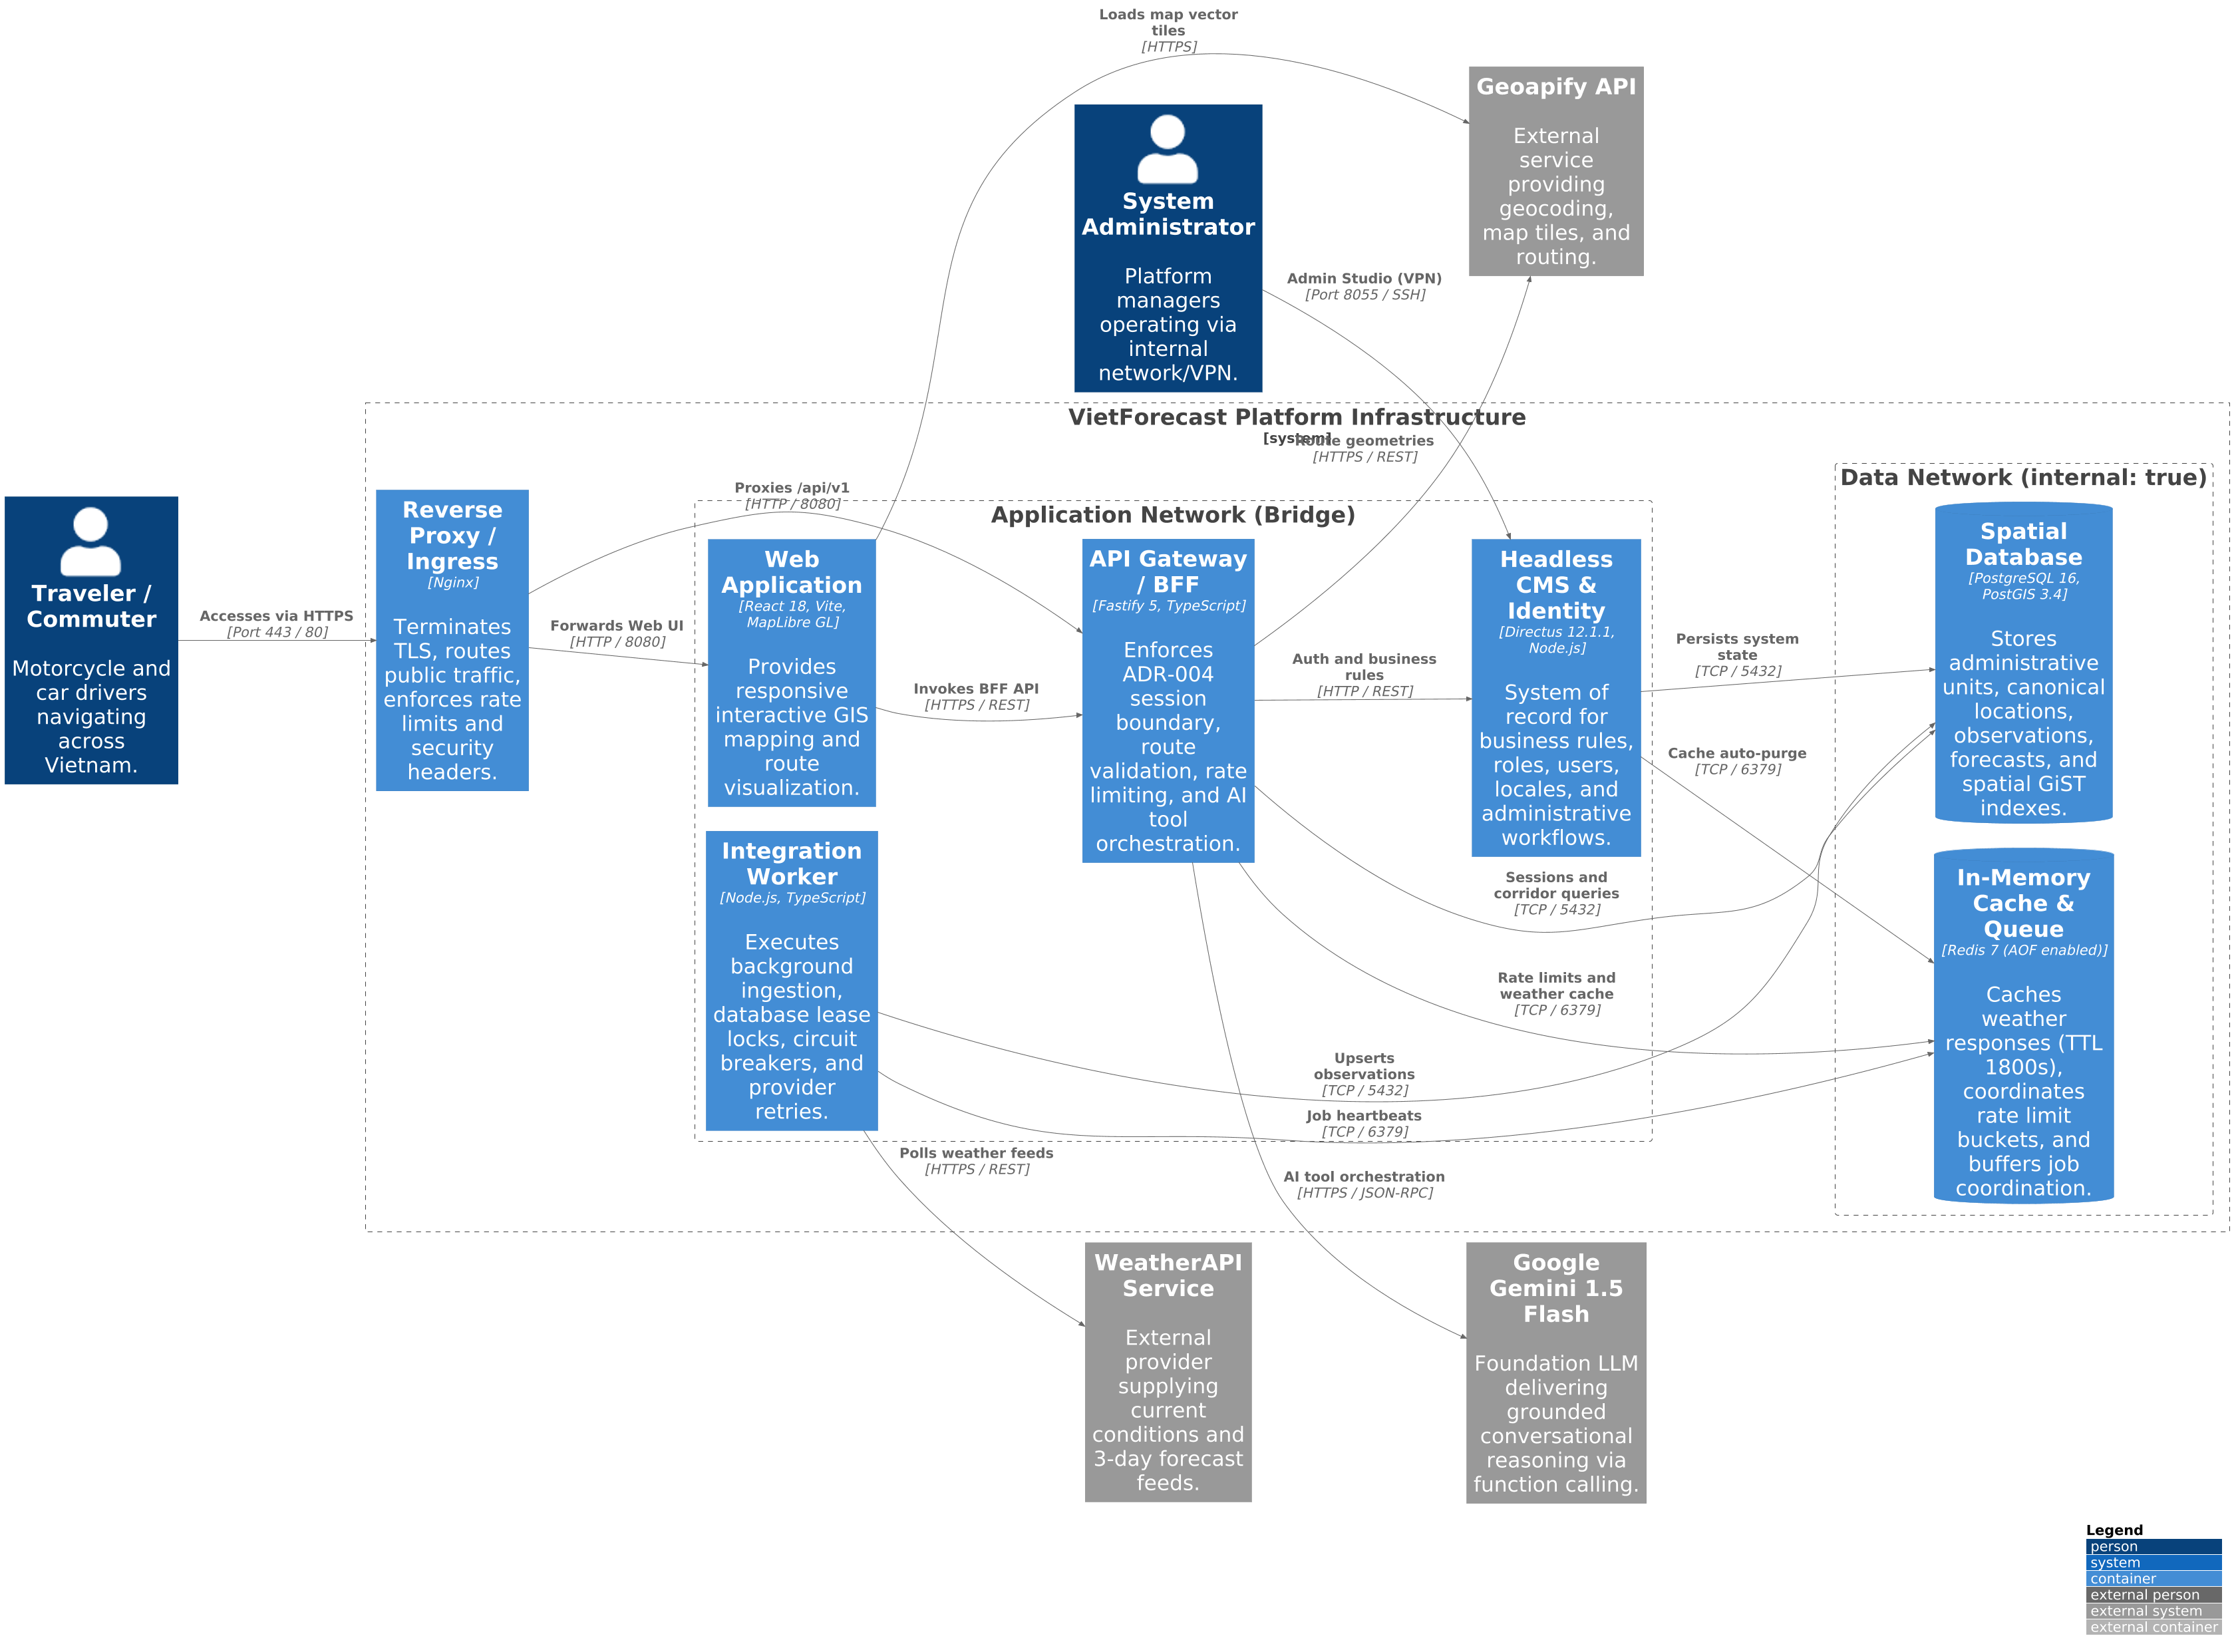
\includegraphics[width=0.95\textwidth, height=0.72\textheight, keepaspectratio]{figures/c4_container.png}
\caption[Biểu đồ C4 Container (Level 2) của VietForecast]{Biểu đồ C4 Container (Level 2) thể hiện cấu trúc microservices và phân vùng mạng của hệ thống VietForecast.}
\label{fig:c4_container_vi}
\end{figure}

Trách nhiệm kỹ thuật của từng container trong hệ thống được phân định rõ ràng theo nguyên tắc phân tách mối quan tâm (Separation of Concerns):
\begin{itemize}
    \item[-] Cổng đảo ngược và kết thúc mã hóa (\textit{Nginx Reverse Proxy}): Đóng vai trò là điểm tiếp nhận lưu lượng duy nhất từ Internet công cộng qua các cổng tiêu chuẩn 80 và 443. Thành phần này chịu trách nhiệm kết thúc phiên TLS/HTTPS, thiết lập các tiêu đề an ninh nghiêm ngặt (Content Security Policy, Strict-Transport-Security, X-Frame-Options), điều phối lưu lượng đến ứng dụng giao diện hoặc cổng giao tiếp API, và thực thi giới hạn lưu lượng truy cập ở cấp độ mạng để bảo vệ hạ tầng phía sau.
    \item[-] Ứng dụng giao diện web người dùng (\textit{Web Application}): Được phát triển dưới dạng ứng dụng trang đơn (Single Page Application) sử dụng React 18, trình đóng gói Vite và thư viện MapLibre GL 4. Ứng dụng cung cấp trải nghiệm tương tác bản đồ không gian mượt mà với tần số quét 60 khung hình trên giây nhờ tăng tốc phần cứng WebGL, trực quan hóa các lớp phủ khí tượng raster và hiển thị đa tuyến lộ trình ba chiều. Ứng dụng hoàn toàn không lưu trữ bất kỳ khóa bí mật API nào của nhà cung cấp bên thứ ba và không tiếp cận trực tiếp cơ sở dữ liệu.
    \item[-] Cổng giao tiếp dịch vụ và Điều phối nghiệp vụ (\textit{Fastify API / BFF}): Xây dựng trên nền tảng Fastify 5 và ngôn ngữ TypeScript, đóng vai trò là tầng trung gian Backend-For-Frontend (BFF). Thành phần này tiếp nhận các yêu cầu từ giao diện web, thực thi xác thực phiên làm việc, phân quyền người dùng, kiểm tra hạn mức sử dụng (rate limiting), điều phối thuật toán đánh giá rủi ro tuyến đường và làm cầu nối bảo mật gọi hàm có kiểm chứng (function calling) tới mô hình ngôn ngữ lớn Google Gemini 1.5 Flash.
    \item[-] Hệ quản trị nội dung và Danh tính người dùng (\textit{Directus 12.1.1}): Đóng vai trò là nguồn dữ liệu chân lý nghiệp vụ (System of Record) cho hệ thống tài khoản, phân quyền dựa trên vai trò (RBAC), danh mục đơn vị hành chính 63 tỉnh thành, các ngưỡng quy tắc rủi ro và nội dung bản địa hóa đa ngôn ngữ. Phiên bản Directus được ấn định chính xác ở bản phát hành 12.1.1 nhằm duy trì tính ổn định tuyệt đối về mặt lược đồ dữ liệu và giao diện quản trị Directus Admin Studio.
    \item[-] Tiến trình xử lý nền tích hợp (\textit{Integration Worker}): Là dịch vụ Node.js chạy độc lập, chịu trách nhiệm thực thi các tác vụ định kỳ có độ trễ cao và phụ thuộc mạng ngoài, bao gồm: thu thập dữ liệu thời tiết bề mặt và dự báo từ WeatherAPI, chuẩn hóa dữ liệu theo quy chuẩn WMO, tính toán giá trị băm kiểm tra tính toàn vẹn SHA-256, và cập nhật trạng thái làm mới vào cơ sở dữ liệu không gian.
    \item[-] Cơ sở dữ liệu không gian quan hệ (\textit{PostgreSQL 16 + PostGIS 3.4}): Là kho lưu trữ dữ liệu bền vững duy nhất của hệ thống, hỗ trợ các kiểu dữ liệu hình học OGC và thuật toán tính toán cung trắc địa elipxoit. Chỉ mục không gian GiST (Generalized Search Tree) được thiết lập trên toàn bộ các cột tọa độ và ranh giới để bảo đảm tốc độ truy vấn hành lang đệm đạt thời gian đáp ứng dưới 50 mili-giây.
    \item[-] Bộ đệm trong bộ nhớ và Điều phối luồng (\textit{Redis 7}): Vận hành với cơ chế ghi nhật ký thay đổi liên tục AOF (Append-Only File), cung cấp bộ nhớ đệm truy xuất tốc độ cực cao cho dữ liệu thời tiết hiện tại (thời gian sống TTL 1.800 giây), điều phối thuật toán Token Bucket kiểm soát tần suất gọi API, và lưu trữ trạng thái đồng bộ giữa các cụm tiến trình.
\end{itemize}

\subsection{Chính sách Phân vùng Mạng và An ninh Mạng Nội bộ (Docker Network Segmentation)}
Để triệt tiêu nguy cơ tấn công lan truyền khi một thành phần bị xâm nhập, hạ tầng vùng chứa Docker của VietForecast thiết lập chính sách phân vùng mạng nghiêm ngặt với hai phân đoạn mạng độc lập:
\begin{itemize}
    \item[-] Phân đoạn mạng ứng dụng nội bộ (\texttt{application} network): Là mạng cầu nối (bridge network) phục vụ việc truyền thông nghiệp vụ giữa Nginx, Web frontend, Fastify API, Directus và Integration Worker. Các dịch vụ trong phân vùng này có thể gửi và nhận các yêu cầu HTTP/REST nội bộ thông qua tên miền dịch vụ được Docker DNS giải quyết cục bộ.
    \item[-] Phân đoạn mạng dữ liệu cô lập tuyệt đối (\texttt{data} network với chỉ thị \texttt{internal: true}): Đây là phân vùng mạng an ninh cấp cao nhất của hệ thống. Chỉ thị \texttt{internal: true} ngăn chặn hoàn toàn việc phân bổ cổng ra ngoài bảng định tuyến Internet của máy chủ chủ (host). Cổng 5432 của PostgreSQL và cổng 6379 của Redis chỉ lắng nghe trên mạng nội bộ này, hoàn toàn vô hình trước môi trường bên ngoài. Bất kỳ nỗ lực quét cổng hay tấn công dò quét mật khẩu từ Internet vào tầng cơ sở dữ liệu đều bị triệt tiêu từ cấp độ định tuyến mạng vùng chứa.
\end{itemize}

Bên cạnh đó, giao diện quản trị Directus Admin Studio (lắng nghe tại cổng 8055) được cấu hình liên kết vòng lặp cục bộ (loopback binding \texttt{127.0.0.1:8055}) theo quy chuẩn an ninh ADR-002 và OPS-010. Người quản trị hệ thống bắt buộc phải thiết lập đường hầm bảo mật SSH (SSH Tunnel) hoặc kết nối qua mạng riêng ảo nội bộ (VPN) mới có thể truy cập trang quản trị, ngăn chặn nguy cơ bị tấn công brute-force hoặc khai thác lỗ hổng zero-day trên giao diện quản trị công khai.

\section{Thiết kế Ranh giới Phiên Bảo mật và An ninh Danh tính (ADR-004)}
\label{sec:auth_session_boundary}

\subsection{Phân tích Nguy cơ Đánh cắp Token và Kiến trúc Ranh giới Phiên BFF}
\label{subsec:token_threat_analysis_vi}
Trong các kiến trúc Single Page Application (SPA) truyền thống, mã xác thực JSON Web Token (Access Token và Refresh Token) \cite{rfc7519} thường được lưu trữ trực tiếp trong bộ nhớ trình duyệt (\texttt{localStorage} hoặc \texttt{sessionStorage}). Kiến trúc này bộc lộ lỗ hổng an ninh chí mạng: bất kỳ cuộc tấn công tiêm mã độc kịch bản chéo trang (Cross-Site Scripting -- XSS) nào bắt nguồn từ các gói phụ thuộc bên thứ ba đều cho phép mã độc chiếm đoạt trực tiếp JWT, dẫn tới việc mạo danh tài khoản mà máy chủ không thể phát hiện hay ngăn chặn. Ngoài ra, việc để máy khách giao tiếp trực tiếp với dịch vụ định danh Directus làm lộ cấu trúc lược đồ dữ liệu nội bộ và tạo sự gắn kết lỏng lẻo về mặt bảo mật.

Để khắc phục triệt để, nền tảng VietForecast thiết lập mô hình Backend-For-Frontend (BFF) thông qua Fastify API theo quyết định kiến trúc ADR-004. Fastify đóng vai trò là ranh giới phiên bảo mật duy nhất: toàn bộ việc giao tiếp với Directus diễn ra trong mạng nội bộ, trong khi trình duyệt tuyệt đối không bao giờ được tiếp cận hay lưu trữ mã JWT thô.

\subsection{Cơ chế Phong bì Mã hóa AES-256-GCM và Khóa Phiên Đục mờ}
\label{subsec:crypto_envelope_vi}
Hệ thống hiện thực hóa nguyên lý phân lập token nghiêm ngặt (\textit{Token Isolation}) và phòng thủ chiều sâu (\textit{Defense-in-Depth}) thông qua mô hình phong bì mật mã ba lớp:
\begin{itemize}
    \item[-] Khóa phiên ngẫu nhiên đục mờ (\textit{Opaque Session Handle}): Máy chủ Fastify phát sinh một chuỗi ngẫu nhiên giả mật mã dài 32 byte ($256\text{ bits}$) sử dụng bộ sinh số ngẫu nhiên CSPRNG (\texttt{createOpaque}\allowbreak\texttt{Token(32)}). Khóa phiên này được gửi về máy khách qua cookie \texttt{\_\_Host-\allowbreak vnwa\_\allowbreak session} với bốn cờ an ninh tối cao: \texttt{HttpOnly} (ngăn chặn JavaScript đọc qua \texttt{document.}\allowbreak\texttt{cookie}), \texttt{Secure} (bắt buộc truyền trên TLS/HTTPS), \texttt{SameSite=Strict} (vô hiệu hóa CSRF), và tiền tố \texttt{\_\_Host-} (khóa cookie vào đúng nguồn gốc tên miền).
    \item[-] Cơ chế băm khóa phiên một chiều (\textit{Token Hashing Pattern}): Nhằm bảo vệ trạng thái phiên ngay cả khi cơ sở dữ liệu bị trích xuất trái phép, máy chủ không lưu trực tiếp khóa đục mờ ở dạng rõ mà băm qua SHA-256 trước khi lưu vào bảng \texttt{app\_security.}\allowbreak\texttt{sessions}:
    \begin{equation}
    \label{eq:session_hash_vi}
    H_{\text{session}} = \text{SHA-256}(\text{handle})
    \end{equation}
    Bản băm $H_{\text{session}}$ dài 64 ký tự thập lục phân đóng vai trò là khóa chính (\texttt{session\_}\allowbreak\texttt{id\_}\allowbreak\texttt{hash}). Kẻ tấn công nếu chiếm được cơ sở dữ liệu cũng không thể giải mã ngược để tái tạo cookie phiên hợp lệ.
    \item[-] Phong bì mã hóa xác thực đối xứng AES-256-GCM (\textit{Authenticated Encryption Envelope}): Cặp mã Directus Access Token và Refresh Token được mã hóa phía máy chủ bằng thuật toán AES-256-GCM với khóa bí mật 256-bit ($K_{\text{enc}} \in \{0, 1\}^{256}$) do Fastify quản lý:
    \begin{equation}
    \label{eq:aes_gcm_vi}
    \mathcal{C} = \text{AES-GCM-Enc}_{K_{\text{enc}}}(P, \text{IV}), \quad \text{Tag} = \text{GCM-Mac}_{K_{\text{enc}}}(\mathcal{C}, \text{IV})
    \end{equation}
    Mỗi chu kỳ tạo hoặc xoay vòng khóa đều sinh một vectơ khởi tạo $\text{IV} \in \{0, 1\}^{96}$ (12 byte) ngẫu nhiên duy nhất và thẻ xác thực $\text{Tag} \in \{0, 1\}^{128}$ (16 byte). Cấu trúc phong bì lưu trữ tuần tự:
    \begin{equation}
    \label{eq:envelope_format_vi}
    \text{Envelope} = \texttt{v1} \,\|\, \text{base64url}(\text{IV}) \,\|\, \text{base64url}(\text{Tag}) \,\|\, \text{base64url}(\mathcal{C})
    \end{equation}
    Bản mã hóa và thẻ xác thực được lưu trữ bền vững trong bảng \texttt{app\_security.}\allowbreak\texttt{sessions}, với quyền truy cập chỉ phân bổ độc quyền cho tài khoản dịch vụ Fastify (\texttt{API\_}\allowbreak\texttt{DB\_}\allowbreak\texttt{USER}).
\end{itemize}

\subsection{Vòng đời Phiên Toàn diện: Cấp phát, Xoay vòng Trượt và Thu hồi Đồng bộ}
\label{subsec:auth_lifecycle_vi}
Vòng đời phiên bảo mật của người dùng được điều phối theo ba giai đoạn tuần tự và khép kín: xác thực cấp phát ban đầu, xoay vòng phiên trượt trơn tru trong quá trình tương tác, và thu hồi đồng bộ tức thời khi kết thúc phiên hoặc phát hiện bất thường an ninh.

\subsubsection{Giai đoạn 1: Xác thực danh tính và cấp phát khóa phiên đục mờ}
Hình~\ref{fig:seq_auth_lifecycle_p1_vi} biểu diễn chi tiết biểu đồ tuần tự của quy trình xác thực đăng nhập người dùng, cơ chế phân xử vai trò RBAC, bảo vệ chống cạn kiệt phiên và cấp phát cookie bảo mật \texttt{\_\_Host-\allowbreak vnwa\_\allowbreak session}.

\begin{figure}[H]
\centering
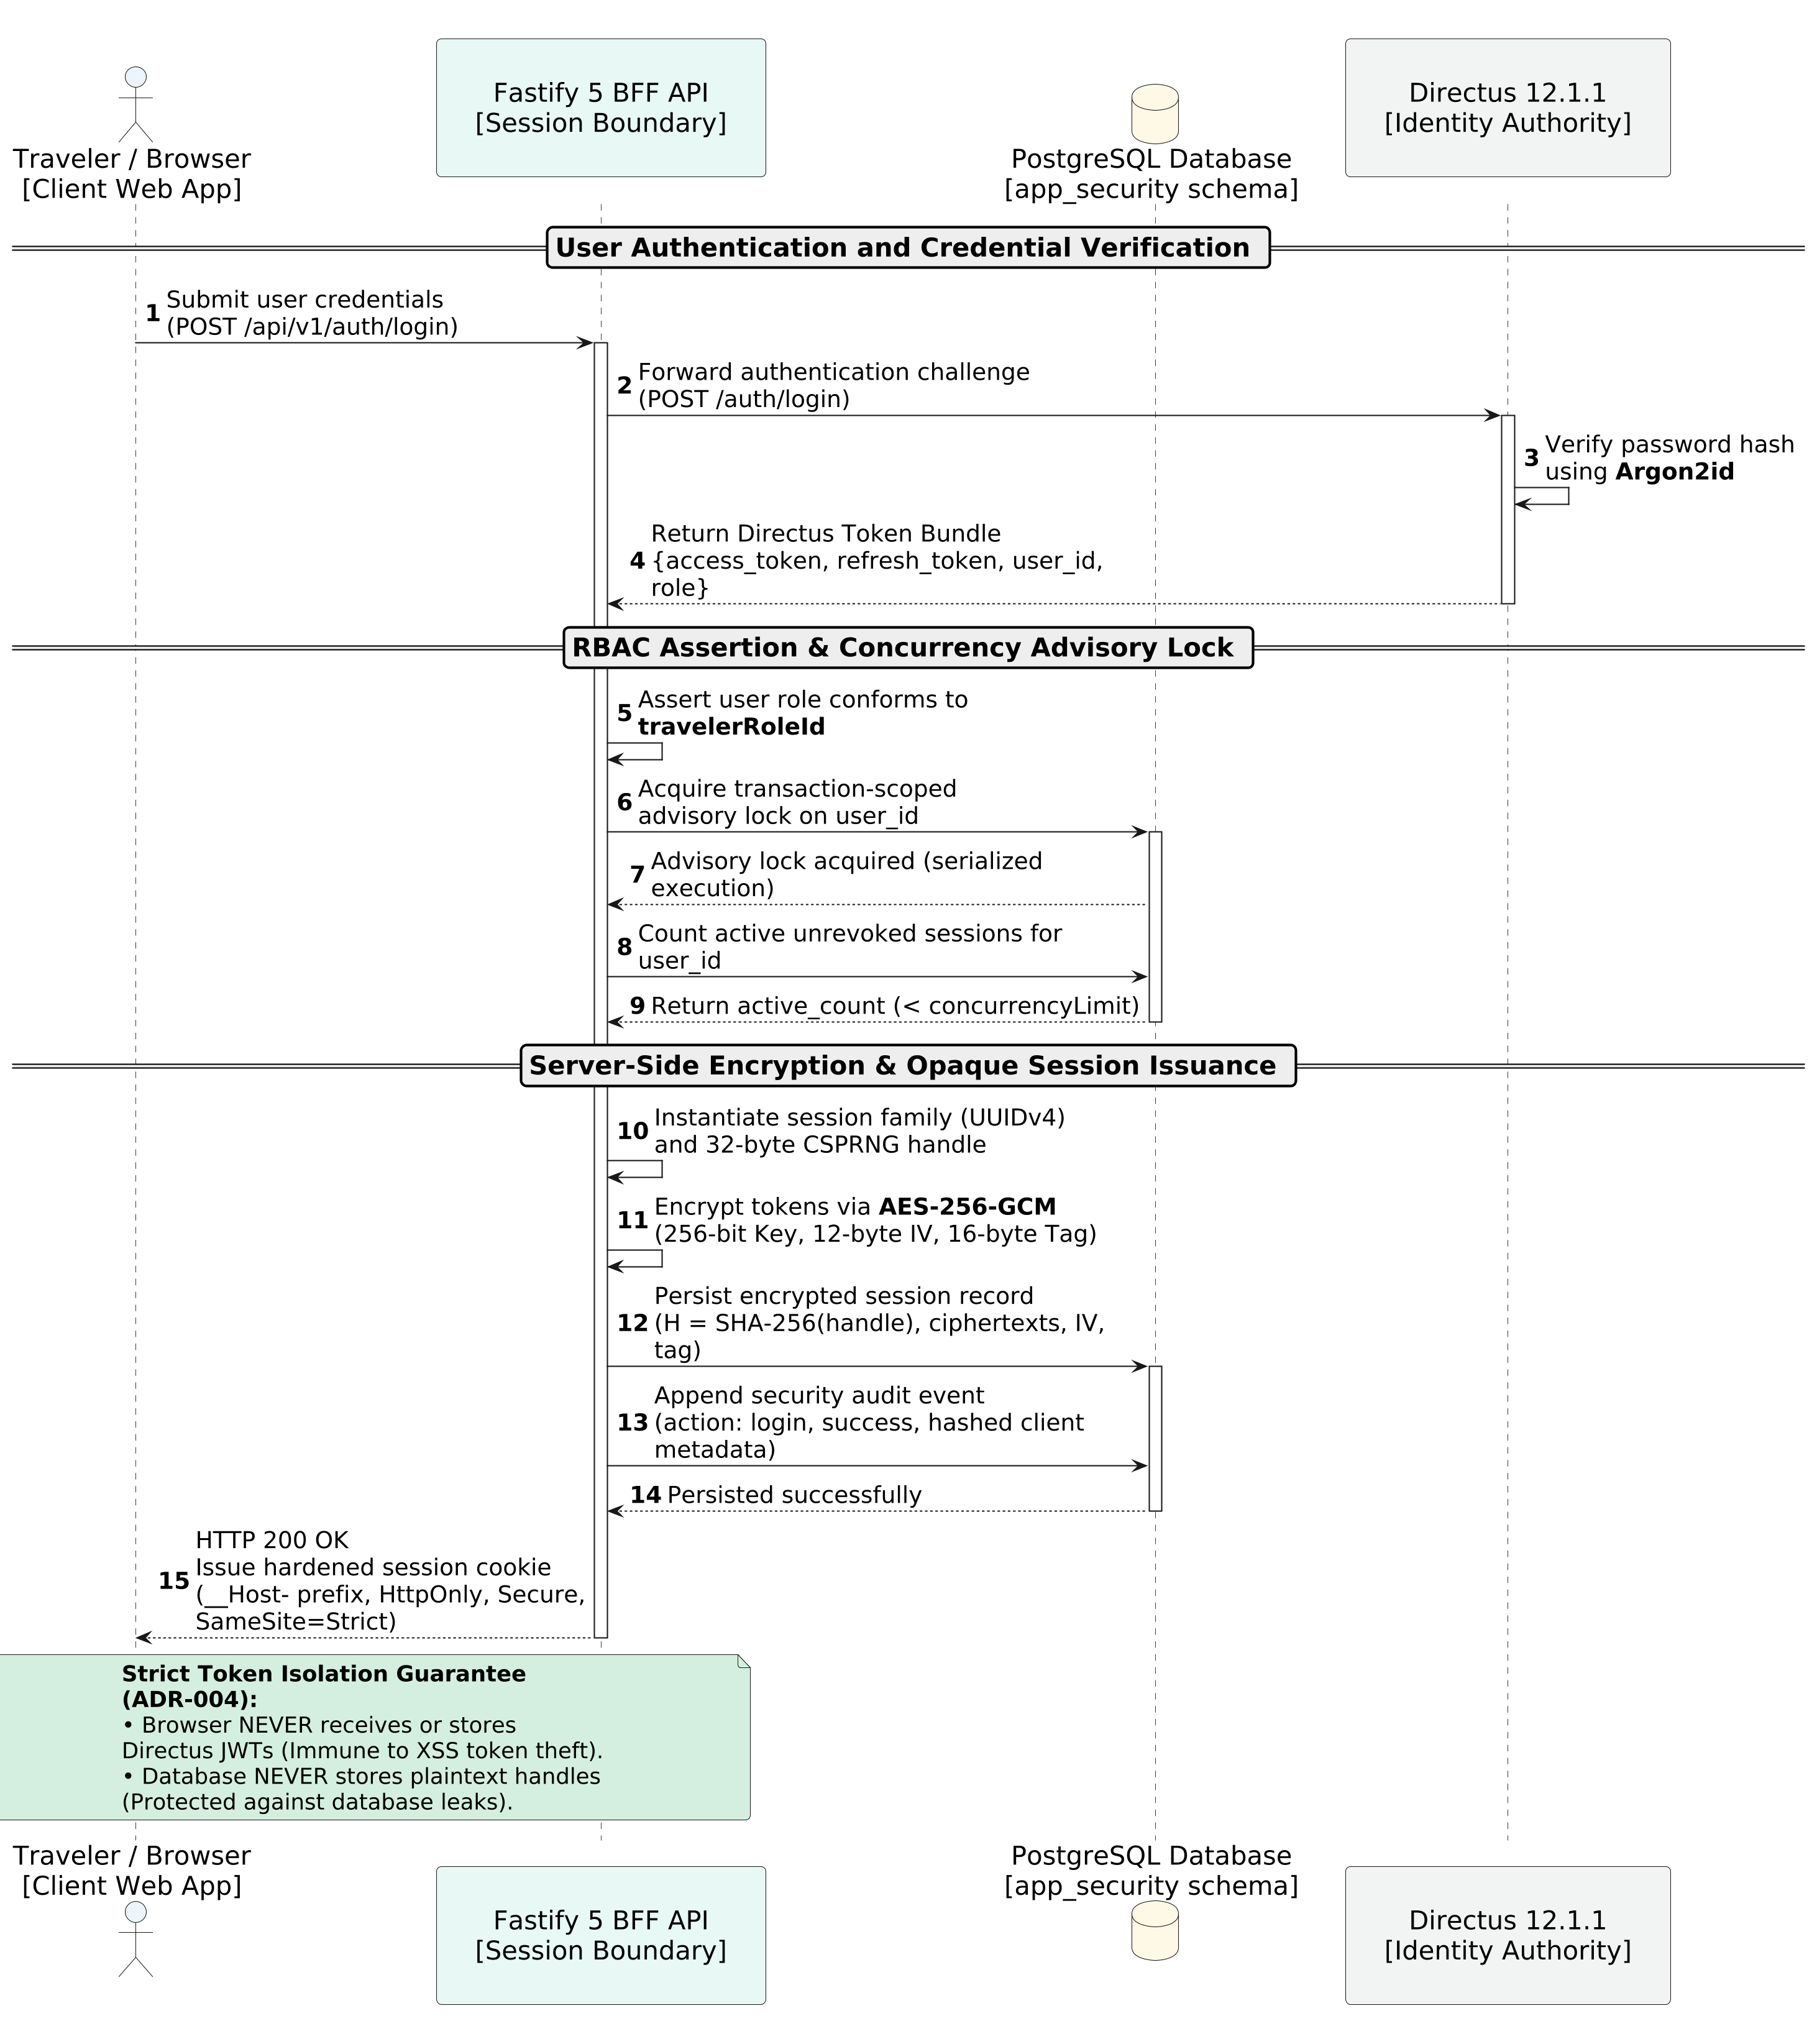
\includegraphics[width=0.92\textwidth, keepaspectratio]{figures/seq_auth_login.png}
\caption[Biểu đồ tuần tự vòng đời phiên (ADR-004) - Giai đoạn 1: Cấp phát khóa phiên]{Biểu đồ tuần tự vòng đời phiên (ADR-004) -- Giai đoạn 1: Xác thực đăng nhập người dùng, cơ chế phân xử vai trò RBAC, kiểm soát phiên đồng thời và cấp phát khóa phiên đục mờ.}
\label{fig:seq_auth_lifecycle_p1_vi}
\end{figure}

Flow hoạt động của Giai đoạn 1 diễn ra qua các bước tuần tự chuẩn hóa:
\begin{itemize}
    \item[-] \textit{Bước 1 (Gửi chứng thực đăng nhập)}: Người dùng nhập thông tin chứng thực (email và mật khẩu) trên ứng dụng giao diện web. Trình duyệt gửi yêu cầu \texttt{POST /api/v1/auth/login} tới cổng Fastify API. Fastify thực thi kiểm tra giới hạn tần suất gọi (Leaky Bucket, 5 req/phút) để ngăn chặn tấn công dò quét mật khẩu.
    \item[-] \textit{Bước 2 (Ủy nhiệm xác thực danh tính)}: Fastify chuyển tiếp thông tin tới Directus Identity Authority qua mạng nội bộ \texttt{application}. Directus kiểm tra mật khẩu đối chiếu với bản băm an toàn theo thuật toán Argon2id. Khi thông tin hợp lệ, Directus phát hành gói mã token gồm Access Token ngắn hạn, Refresh Token dài hạn, mã định danh người dùng và vai trò phân quyền.
    \item[-] \textit{Bước 3 (Thẩm định RBAC và khóa tư vấn phiên đồng thời)}: Fastify kiểm tra vai trò người dùng thuộc đúng nhóm \texttt{travelerRoleId}. Để ngăn chặn tấn công chiếm dụng tài nguyên phiên hoặc vượt quá số lượng thiết bị cho phép, hệ thống tuần tự hóa nguyên tử việc kiểm tra số lượng phiên hoạt động của người dùng $u$ thông qua khóa tư vấn cấp giao dịch (transaction-scoped advisory lock) liên kết với giá trị băm $h_u = \text{Hash}_{64}(u)$:
    \begin{equation}
    \label{eq:concurrency_bound_vi}
    N_{\text{active}}(u) = \Big| \big\{ s \in \mathcal{S} \;\big|\; s.\text{user\_id} = u \;\wedge\; s.\text{revoked\_at} = \emptyset \big\} \Big| < C_{\text{limit}}
    \end{equation}
    Nếu số lượng phiên chạm ngưỡng quy định $C_{\text{limit}}$, hệ thống tự động vô hiệu hóa phiên cũ nhất để giải phóng tài nguyên.
    \item[-] \textit{Bước 4 (Mã hóa phong bì AES-256-GCM và sinh khóa đục mờ)}: Fastify sinh định danh họ phiên mới (UUIDv4) cùng khóa phiên đục mờ ngẫu nhiên dài 32 byte ($h$) từ bộ sinh số ngẫu nhiên CSPRNG. Cặp mã JWT được đóng gói và mã hóa đối xứng phía máy chủ bằng thuật toán AES-256-GCM với vectơ khởi tạo ngẫu nhiên 12 byte ($\text{IV} \in \{0, 1\}^{96}$) và thẻ xác thực 16 byte ($\text{Tag} \in \{0, 1\}^{128}$) theo Khóa mã hóa máy chủ $K_{\text{enc}}$.
    \item[-] \textit{Bước 5 (Lưu trữ bản băm một chiều và ghi nhật ký kiểm toán)}: Fastify tính bản băm một chiều $H_{\text{session}} = \text{SHA-256}(h)$ và ghi bản ghi phiên vào bảng \texttt{app\_security.sessions}. Đồng thời, một bản ghi kiểm toán bất biến được ghi nhận vào bảng \texttt{app\_}\allowbreak\texttt{security.}\allowbreak\texttt{audit\_}\allowbreak\texttt{events} với hành động đăng nhập thành công kèm siêu dữ liệu máy khách đã băm bảo vệ quyền riêng tư.
    \item[-] \textit{Bước 6 (Phát hành cookie bảo mật)}: Fastify trả về phản hồi thành công (HTTP 200 OK) và thiết lập cookie phiên bảo mật \texttt{\_\_Host-vnwa\_session} trên trình duyệt với cờ \texttt{HttpOnly} (ngăn chặn JavaScript đọc cookie), cờ \texttt{Secure} (bắt buộc truyền tải trên kênh TLS), cờ \texttt{SameSite=Strict} (triệt tiêu tấn công CSRF) và tiền tố \texttt{\_\_Host-} (ràng buộc tuyệt đối nguồn gốc tên miền).
\end{itemize}

\subsubsection{Giai đoạn 2: Xử lý yêu cầu ủy quyền và xoay vòng phiên trượt trơn tru}
Hình~\ref{fig:seq_auth_lifecycle_p2_vi} minh họa chi tiết biểu đồ tuần tự của quy trình tiếp nhận yêu cầu ủy quyền nghiệp vụ và cơ chế xoay vòng phiên trượt ngầm (Silent Sliding Rotation).

\begin{figure}[H]
\ContinuedFloat
\centering
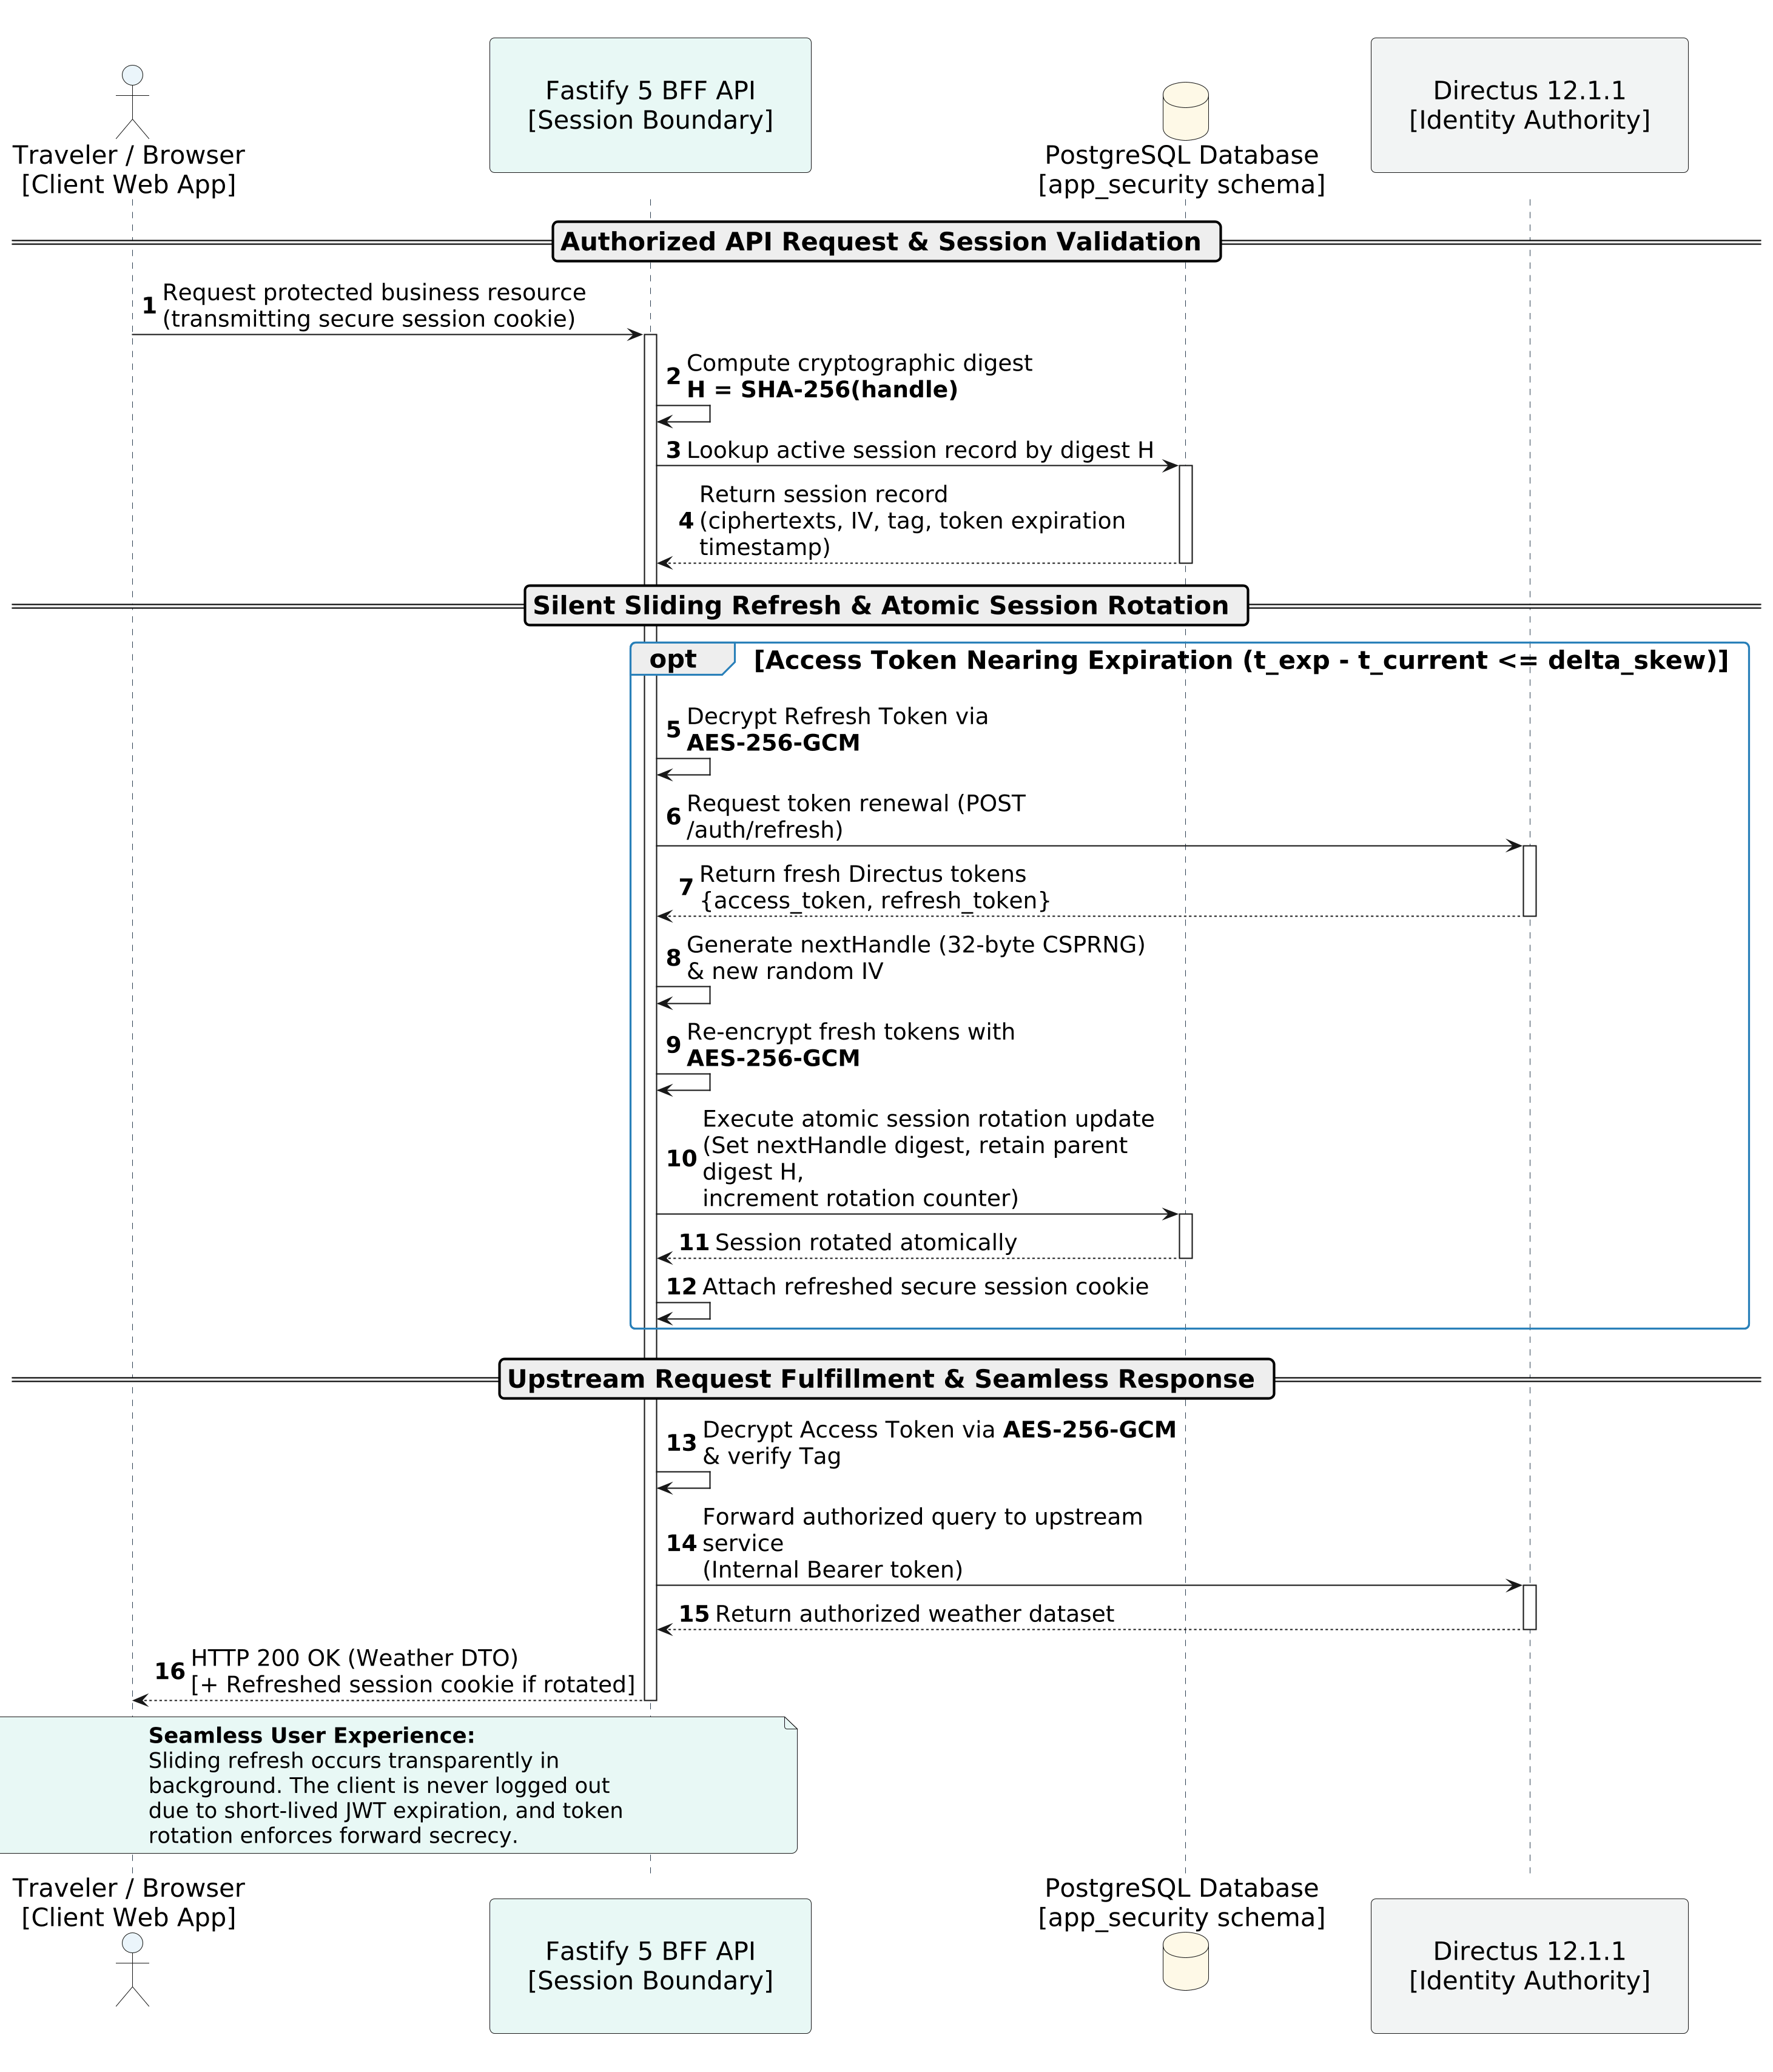
\includegraphics[width=0.92\textwidth, keepaspectratio]{figures/seq_sliding_rotation.png}
\caption[Biểu đồ tuần tự vòng đời phiên (ADR-004) - Giai đoạn 2: Xoay vòng trượt ngầm]{Biểu đồ tuần tự vòng đời phiên (ADR-004) (tiếp theo) -- Giai đoạn 2: Xử lý yêu cầu ủy quyền nghiệp vụ và cơ chế xoay vòng phiên trượt trơn tru (Silent Sliding Rotation).}
\label{fig:seq_auth_lifecycle_p2_vi}
\end{figure}

Flow hoạt động của Giai đoạn 2 được thiết kế như sau:
\begin{itemize}
    \item[-] \textit{Bước 1 (Đón bắt cookie và đối chiếu bản băm)}: Khi máy khách gửi yêu cầu nghiệp vụ kèm theo cookie \texttt{\_\_Host-\allowbreak vnwa\_\allowbreak session}, tầng chặn bắt an ninh của Fastify trích xuất chuỗi định danh phiên $h$, tính bản băm $H = \text{SHA-256}(h)$, và đối chiếu với tập trạng thái phiên trong cơ sở dữ liệu (hoặc bộ đệm Redis). Nếu không tồn tại bản ghi hợp lệ hoặc phiên đã bị đánh dấu thu hồi, yêu cầu lập tức bị từ chối với mã lỗi HTTP 401 Unauthorized.
    \item[-] \textit{Bước 2 (Đánh giá cửa sổ dung sai làm mới trượt)}: Sau khi xác thực phiên hợp lệ, Fastify kiểm tra thời hạn sống còn lại của Access Token trong phong bì mã hóa. Nếu khoảng cách từ thời điểm hiện tại $t_{\text{current}}$ đến mốc hết hạn $t_{\text{exp}}$ nhỏ hơn hoặc bằng ngưỡng dung sai làm mới $\Delta t_{\text{skew}}$:
    \begin{equation}
    \label{eq:sliding_skew_vi}
    t_{\text{exp}} - t_{\text{current}} \le \Delta t_{\text{skew}}
    \end{equation}
    hệ thống tự động kích hoạt luồng làm mới phiên trượt ngầm hoàn toàn trong suốt với người dùng.
    \item[-] \textit{Bước 3 (Đổi token và chuyển dịch trạng thái nguyên tử)}: Fastify sử dụng khóa $K_{\text{enc}}$ giải mã Refresh Token bằng thuật toán AES-256-GCM và gọi nội bộ sang Directus để đổi lấy cặp token mới. Ngay sau khi nhận cặp token mới, Fastify sinh một khóa phiên đục mờ kế tiếp $h_{k+1}$ dài 32 byte và vectơ khởi tạo $\text{IV}_{k+1}$ mới để tái mã hóa gói dữ liệu. Quá trình xoay vòng chuyển dịch trạng thái nguyên tử qua toán tử $\mathcal{T}_{\text{rotate}}$:
    \begin{equation}
    \label{eq:rotate_session_vi}
    \begin{aligned}
    \mathcal{T}_{\text{rotate}}(S_k) \xrightarrow{\text{nguyên tử}} S_{k+1} = \big\langle & \text{SHA-256}(h_{k+1}),\; \mathcal{C}_{k+1}, \\
    & \text{IV}_{k+1},\; \text{Tag}_{k+1},\; t_{\text{exp}, k+1},\; c_k + 1 \big\rangle
    \end{aligned}
    \end{equation}
    đồng thời duy trì liên kết phả hệ khóa cha để phát hiện tấn công tái sử dụng:
    \begin{equation}
    \label{eq:rotate_lineage_vi}
    S_{k+1}.\text{ancestor\_hash} = H_k
    \end{equation}
    \item[-] \textit{Bước 4 (Thời gian ân hạn và hoàn tất yêu cầu nghiệp vụ)}: Khóa phiên cũ $h_k$ được duy trì trong một khoảng thời gian ân hạn ngắn ($\text{TTL}_{\text{grace}} = 60\text{ s}$) trong Redis nhằm xử lý các yêu cầu mạng đồng thời đang bay dở dang mà không gây lỗi phiên giả mạo. Fastify giải mã Access Token, gắn vào tiêu đề ủy quyền nội bộ để truy vấn tập dữ liệu thời tiết, và trả kết quả về cho máy khách kèm theo chỉ thị cập nhật cookie phiên mang khóa thế hệ mới $h_{k+1}$.
\end{itemize}

\subsubsection{Giai đoạn 3: Thu hồi phiên đồng bộ và tiêu hủy phả hệ phiên}
Hình~\ref{fig:seq_auth_lifecycle_p3_vi} minh họa biểu đồ tuần tự của cơ chế thu hồi phiên đồng bộ qua Trigger cơ sở dữ liệu và tiêu hủy họ phiên khi phát hiện tái sử dụng token.

\begin{figure}[H]
\ContinuedFloat
\centering
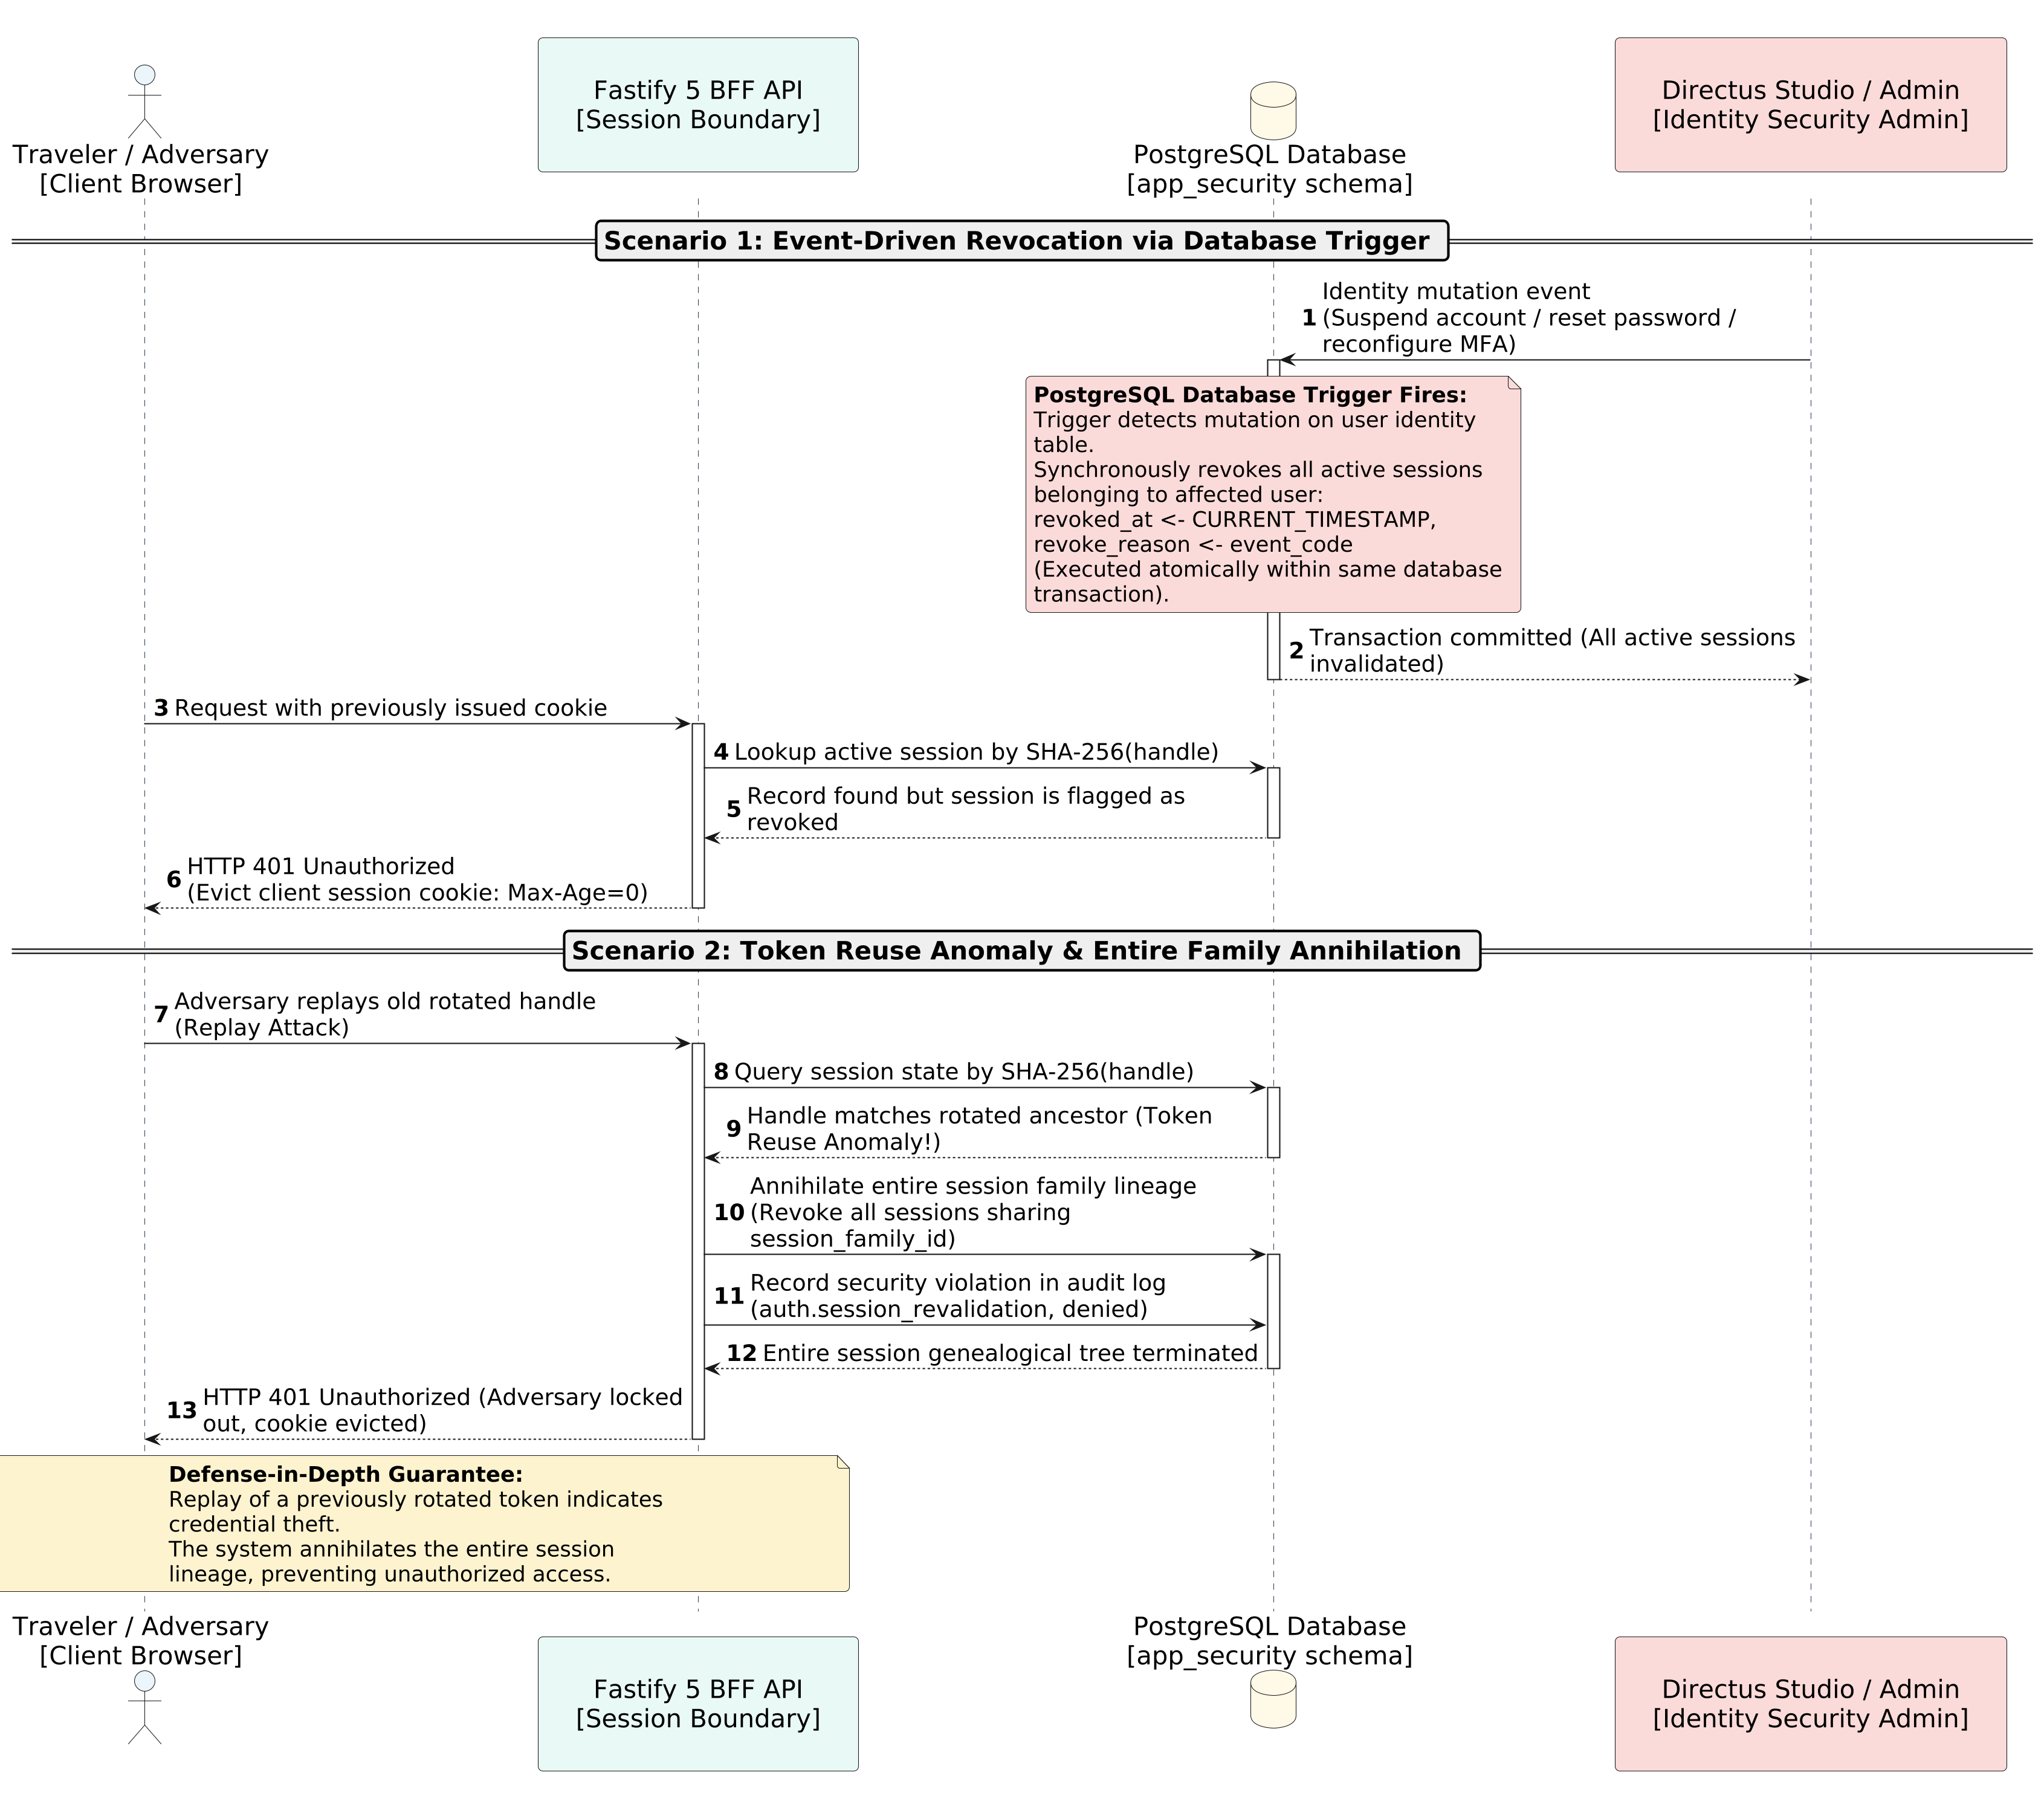
\includegraphics[width=0.92\textwidth, keepaspectratio]{figures/seq_session_revocation.png}
\caption[Biểu đồ tuần tự vòng đời phiên (ADR-004) - Giai đoạn 3: Thu hồi đồng bộ]{Biểu đồ tuần tự vòng đời phiên (ADR-004) (tiếp theo) -- Giai đoạn 3: Thu hồi họ phiên đồng bộ qua Trigger cơ sở dữ liệu và tiêu hủy toàn bộ dòng họ phiên khi phát hiện tái sử dụng token.}
\label{fig:seq_auth_lifecycle_p3_vi}
\end{figure}

Flow hoạt động của Giai đoạn 3 được điều phối qua ba kịch bản phòng thủ chuyên sâu:
\begin{itemize}
    \item[-] \textit{Kịch bản 1 (Thu hồi đồng bộ hướng sự kiện qua Trigger cơ sở dữ liệu)}: Khi người quản trị thực hiện vô hiệu hóa tài khoản trên Directus Studio, hoặc khi người dùng đổi mật khẩu hay cập nhật cấu hình xác thực hai yếu tố (MFA), một biến cố đột biến danh tính xảy ra. Trigger cơ sở dữ liệu tự động kích hoạt toán tử vô hiệu hóa $\Phi_{\text{trigger}}$ trong cùng một giao dịch ACID:
    \begin{equation}
    \label{eq:trigger_revoke_vi}
    \begin{aligned}
    \forall s \in \mathcal{S}, \; (s.\text{user\_id} = u \;\wedge\; s.\text{revoked\_at} = \emptyset) \implies \\
    \Phi_{\text{trigger}}(s) : \begin{cases}
    s.\text{revoked\_at} \leftarrow t_{\text{event}} \\
    s.\text{revoke\_reason} \leftarrow \text{code}_{\text{reason}}
    \end{cases}
    \end{aligned}
    \end{equation}
    trong đó $t_{\text{event}}$ là thời điểm giao dịch danh tính diễn ra, và $\text{code}_{\text{reason}}$ là mã nguyên nhân chuẩn hóa (\texttt{identity\_}\allowbreak\texttt{password\_}\allowbreak\texttt{changed}, \texttt{identity\_}\allowbreak\texttt{status\_}\allowbreak\texttt{changed}, \texttt{identity\_}\allowbreak\texttt{role\_}\allowbreak\texttt{changed}, \texttt{identity\_}\allowbreak\texttt{mfa\_}\allowbreak\texttt{changed}, hoặc \texttt{identity\_}\allowbreak\texttt{deleted}). Toàn bộ các phiên đang hoạt động của người dùng trên mọi thiết bị lập tức bị vô hiệu hóa đồng loạt.
    \item[-] \textit{Kịch bản 2 (Phát hiện tái sử dụng token và tiêu hủy toàn bộ họ phiên)}: Nếu kẻ tấn công đánh cắp được một cookie phiên cũ đã qua xoay vòng và cố gắng gửi yêu cầu sau khi thời gian ân hạn 60 giây đã kết thúc, Fastify phát hiện giá trị băm của cookie trùng khớp với trường lưu vết khóa cha $S.\text{ancestor\_hash}$ của một bản ghi đã tiến hóa. Fastify lập tức kích hoạt toán tử tiêu hủy toàn bộ dòng họ phiên $\Psi_{\text{annihilate}}$:
    \begin{equation}
    \label{eq:family_revoke_vi}
    \begin{aligned}
    \forall s \in \mathcal{S}, \; (s.\text{family\_id} = F_{\text{target}}) \implies \\
    \Psi_{\text{annihilate}}(s) : \begin{cases}
    s.\text{revoked\_at} \leftarrow t_{\text{detection}} \\
    s.\text{revoke\_reason} \leftarrow \text{`token\_reuse\_detected'}
    \end{cases}
    \end{aligned}
    \end{equation}
    Đồng thời, toàn bộ khóa liên đới trong Redis bị xóa sạch và một cảnh báo an ninh nghiêm trọng được ghi vào nhật ký kiểm toán, trung hòa hoàn toàn nguy cơ kẻ tấn công lợi dụng phiên bị rò rỉ.
    \item[-] \textit{Kịch bản 3 (Đăng xuất tự nguyện và thanh trừng định kỳ)}: Khi người dùng bấm đăng xuất (\texttt{POST /auth/logout}), Fastify cập nhật trường \texttt{revoked\_at} trong cơ sở dữ liệu, xóa khóa đệm trong Redis và phát lệnh xóa cookie \texttt{\_\_Host-vnwa\_session} (thiết lập \texttt{Max-Age=0}). Thủ tục dọn dẹp định kỳ chạy ngầm thực hiện thanh trừng vĩnh viễn các bản ghi phiên đã thu hồi vượt quá thời gian lưu trữ bắt buộc.
\end{itemize}

\section{Thiết kế Tiến trình Xử lý Nền Worker và Cơ chế Ổn định Hệ thống (ADR-001)}
\label{sec:worker_resilience_adr001}

\subsection{Phân tách Miền Lỗi Giữa Tác vụ Nền và Giao diện Lập trình Ứng dụng}
Trong quá trình vận hành hệ thống thông tin khí tượng, tác vụ thu thập dữ liệu từ các dịch vụ API bên ngoài (như WeatherAPI) có xác suất gặp lỗi cao do nghẽn mạng quốc tế, quá tải máy chủ cung cấp hoặc cạn kiệt hạn ngạch truy vấn. Hơn nữa, việc thu thập dữ liệu cho toàn bộ 63 tỉnh thành Việt Nam với chu kỳ 15 đến 30 phút một lần tiêu tốn đáng kể thời gian I/O và chu kỳ xử lý chuẩn hóa dữ liệu.

Nếu tích hợp các tác vụ này vào trong cùng một tiến trình ứng dụng API phục vụ người dùng hoặc tận dụng luồng tự động hóa (Directus Flow) kéo dài, hiện tượng tranh chấp tài nguyên (Event Loop Blocking) sẽ xảy ra, làm giảm sút nghiêm trọng tốc độ phản hồi các yêu cầu tương tác giao diện và có thể dẫn đến sự cố sập đổ dây chuyền (Cascading Failure). Do đó, theo quyết định kiến trúc ADR-001, toàn bộ các tác vụ thu thập, chuẩn hóa, tính toán và bảo trì dữ liệu được phân tách hoàn toàn sang một tiến trình xử lý nền độc lập mang tên Integration Worker.

\subsection{Cơ chế Chiếm Khóa Phân tán trên Cơ sở Dữ liệu (Distributed Database Leasing)}
Để ngăn chặn tình trạng nhiều tiến trình worker cùng thực thi thu thập dữ liệu trùng lặp khi hệ thống được mở rộng ngang trên nhiều container hoặc nhiều máy chủ vật lý, hệ thống triển khai cơ chế chiếm khóa phân tán (Distributed Database Leasing) trên bảng \texttt{weather\_worker\_leases} của PostgreSQL.

Cơ chế này hoạt động dựa trên nguyên tắc chiếm quyền độc quyền có thời hạn (atomic acquisition with expiration):
\begin{itemize}
    \item[-] Khi bắt đầu một chu kỳ đồng bộ dữ liệu, worker cố gắng thực thi câu lệnh chèn hoặc cập nhật có điều kiện (\texttt{INSERT ... ON CONFLICT DO UPDATE}) trên bản ghi khóa tài nguyên. Thao tác chỉ thành công nếu chưa có worker nào nắm giữ khóa hoặc khóa hiện tại đã vượt quá thời gian hiệu lực (hết hạn).
    \item[-] Thời gian giữ khóa được quy định bởi tham số \texttt{WEATHER\_}\allowbreak\texttt{WORKER\_}\allowbreak\texttt{LEASE\_}\allowbreak\texttt{DURATION\_MS} ($120.000\text{ ms}$).
    \item[-] Trong suốt quá trình thực thi tác vụ tải dữ liệu và chuẩn hóa, worker định kỳ gửi tín hiệu nhịp tim (\texttt{heartbeat}) sau mỗi 30.000 mili-giây (\texttt{HEARTBEAT\_INTERVAL\_MS} ($30.000\text{ ms}$)) để gia hạn thời điểm hết hạn của khóa.
    \item[-] Trong trường hợp tiến trình worker bị sập nguồn đột ngột hoặc mất kết nối mạng, tín hiệu nhịp tim bị gián đoạn. Khi vượt quá ngưỡng 120 giây, khóa tự động bị coi là hết hạn mà không gây ra tình trạng bế tắc vĩnh viễn (deadlock). Tiến trình worker kế tiếp có thể tiếp quản tài nguyên và thực thi chu kỳ đồng bộ tiếp theo một cách an toàn và tự động.
\end{itemize}

\subsection{Cơ chế Ngắt mạch (Circuit Breaker) và Thử lại Thích ứng}
Để bảo vệ hạn mức truy vấn API thời tiết của hệ thống cũng như duy trì tính sẵn sàng khi dịch vụ ngoài gặp sự cố, tiến trình Integration Worker tích hợp mô hình ngắt mạch (Circuit Breaker Pattern) ba trạng thái:
\begin{itemize}
    \item[-] \textit{Trạng thái Đóng (CLOSED)}: Toàn bộ các yêu cầu gọi sang WeatherAPI được thực thi bình thường. Hệ thống giám sát tỷ lệ lỗi liên tiếp.
    \item[-] \textit{Trạng thái Mở (OPEN)}: Khi số lần gọi thất bại liên tiếp (do lỗi mã phản hồi HTTP 5xx, lỗi quá tải HTTP 429 hoặc vượt quá thời gian chờ \texttt{TIMEOUT\_MS} ($8.000\text{ ms}$)) chạm ngưỡng \texttt{CIRCUIT\_FAILURE\_}\allowbreak\texttt{THRESHOLD} ($3$ lần), bộ ngắt mạch lập tức chuyển sang trạng thái Mở. Trong trạng thái này, mọi yêu cầu thu thập dữ liệu mới bị đình chỉ ngay lập tức tại worker mà không gửi yêu cầu ra mạng bên ngoài, giúp bảo toàn tài nguyên và tránh gây áp lực thêm lên máy chủ nhà cung cấp.
    \item[-] \textit{Trạng thái Bán Mở (HALF-OPEN)}: Sau thời gian chờ \texttt{CIRCUIT\_RESET\_MS} ($60.000\text{ ms}$) (60 giây), bộ ngắt mạch tự động chuyển sang trạng thái Bán Mở và cho phép một yêu cầu thăm dò đơn lẻ được phát đi. Nếu yêu cầu này thành công, mạch quay về trạng thái Đóng; ngược lại nếu tiếp tục thất bại, mạch tái lập trạng thái Mở và khởi động lại chu kỳ đếm thời gian.
\end{itemize}

Đối với các lỗi mang tính nhất thời, worker kích hoạt thuật toán thử lại theo hàm số mũ kết hợp độ trễ ngẫu nhiên (Exponential Backoff with Jitter). Khoảng thời gian trì hoãn giữa các lần thử lại thứ $k$ được tính toán theo công thức:
\begin{equation}
\label{eq:backoff_jitter}
t_{\text{delay}}(k) = \min\left(t_{\max}, \; t_{\text{base}} \cdot 2^{k-1}\right) \cdot \left(1 + r_{\text{jitter}} \cdot \mathcal{U}(-1, 1)\right)
\end{equation}
với độ trễ cơ sở $t_{\text{base}} = 5.000\text{ ms}$, độ trễ trần $t_{\max} = 60.000\text{ ms}$, tỷ lệ độ trễ ngẫu nhiên $r_{\text{jitter}} = 0{,}2$ và $\mathcal{U}(-1, 1)$ là biến ngẫu nhiên phân bố đều trong khoảng $[-1, 1]$. Yếu tố ngẫu nhiên này đóng vai trò quyết định trong việc ngăn chặn hiện tượng nghẽn mạng tập trung (thundering herd problem) khi nhiều trạm thời tiết cùng đồng loạt thử kết nối lại tại một thời điểm.

\subsection{Kiểm soát Vòng đời Độ tươi mới Dữ liệu Khí tượng và Trạng thái An toàn}
Dữ liệu quan trắc sau khi thu thập thành công từ WeatherAPI được chuẩn hóa về hệ thống đơn vị đo lường khí tượng quốc tế (WMO-No. 8) và tính toán mã băm SHA-256 để chống trùng lặp dữ liệu trước khi ghi vào bảng \texttt{weather\_}\allowbreak\texttt{observations}. Đồng thời, worker cập nhật bản ghi trong bảng dự báo \texttt{weather\_forecasts} và phát tín hiệu làm mới bộ nhớ đệm Redis với thời gian sống TTL tương ứng.

Dữ liệu thời tiết lưu trữ trong hệ thống được kiểm soát nghiêm ngặt theo ba trạng thái độ tươi mới nhằm bảo đảm tính an toàn cho động cơ tính điểm rủi ro hành trình:
\begin{itemize}
    \item[-] \textit{Dữ liệu mới (Fresh)}: Độ trễ $\tau \le 60$ phút tính từ thời điểm đo thực tế tại trạm quan trắc. Dữ liệu này được coi là hoàn toàn hợp lệ và phản ánh chính xác tình trạng khí quyển hiện tại, được đưa trực tiếp vào thuật toán đánh giá an toàn lộ trình.
    \item[-] \textit{Dữ liệu cũ (Aging)}: Độ trễ nằm trong khoảng $60 < \tau \le 180$ phút. Hệ thống vẫn cho phép truy vấn phục vụ các tính toán định tuyến nhưng giao diện ứng dụng bắt buộc hiển thị nhãn cảnh báo thời điểm cập nhật cũ để người dùng chủ động lưu ý.
    \item[-] \textit{Dữ liệu hết hạn (Stale)}: Khi độ trễ $\tau > 180$ phút (hoặc trạm quan trắc mất kết nối quá 3 giờ). Theo nguyên tắc thiết kế an toàn tuyệt đối (Fail-Safe Principle), hệ thống kiên quyết từ chối sử dụng dữ liệu này để nội suy rủi ro và tự động ánh xạ mức độ nguy hiểm về trạng thái \texttt{Unknown} (mã màu xám \#9CA3AF), bảo đảm người tham gia giao thông luôn nhận thức rõ việc thiếu dữ liệu thực địa thay vì tin tưởng vào các dự báo an toàn giả tạo.
\end{itemize}

Hình~\ref{fig:seq_ingestion_vi} mô tả chi tiết toàn bộ chu trình vận hành nền của tiến trình Integration Worker, bao gồm cơ chế chiếm quyền khóa phân tán, xử lý ngắt mạch tự động khi có lỗi mạng, khâu kiểm tra toàn vẹn mã băm và cập nhật giao dịch ACID vào hệ thống lưu trữ.

\begin{figure}[H]
\centering
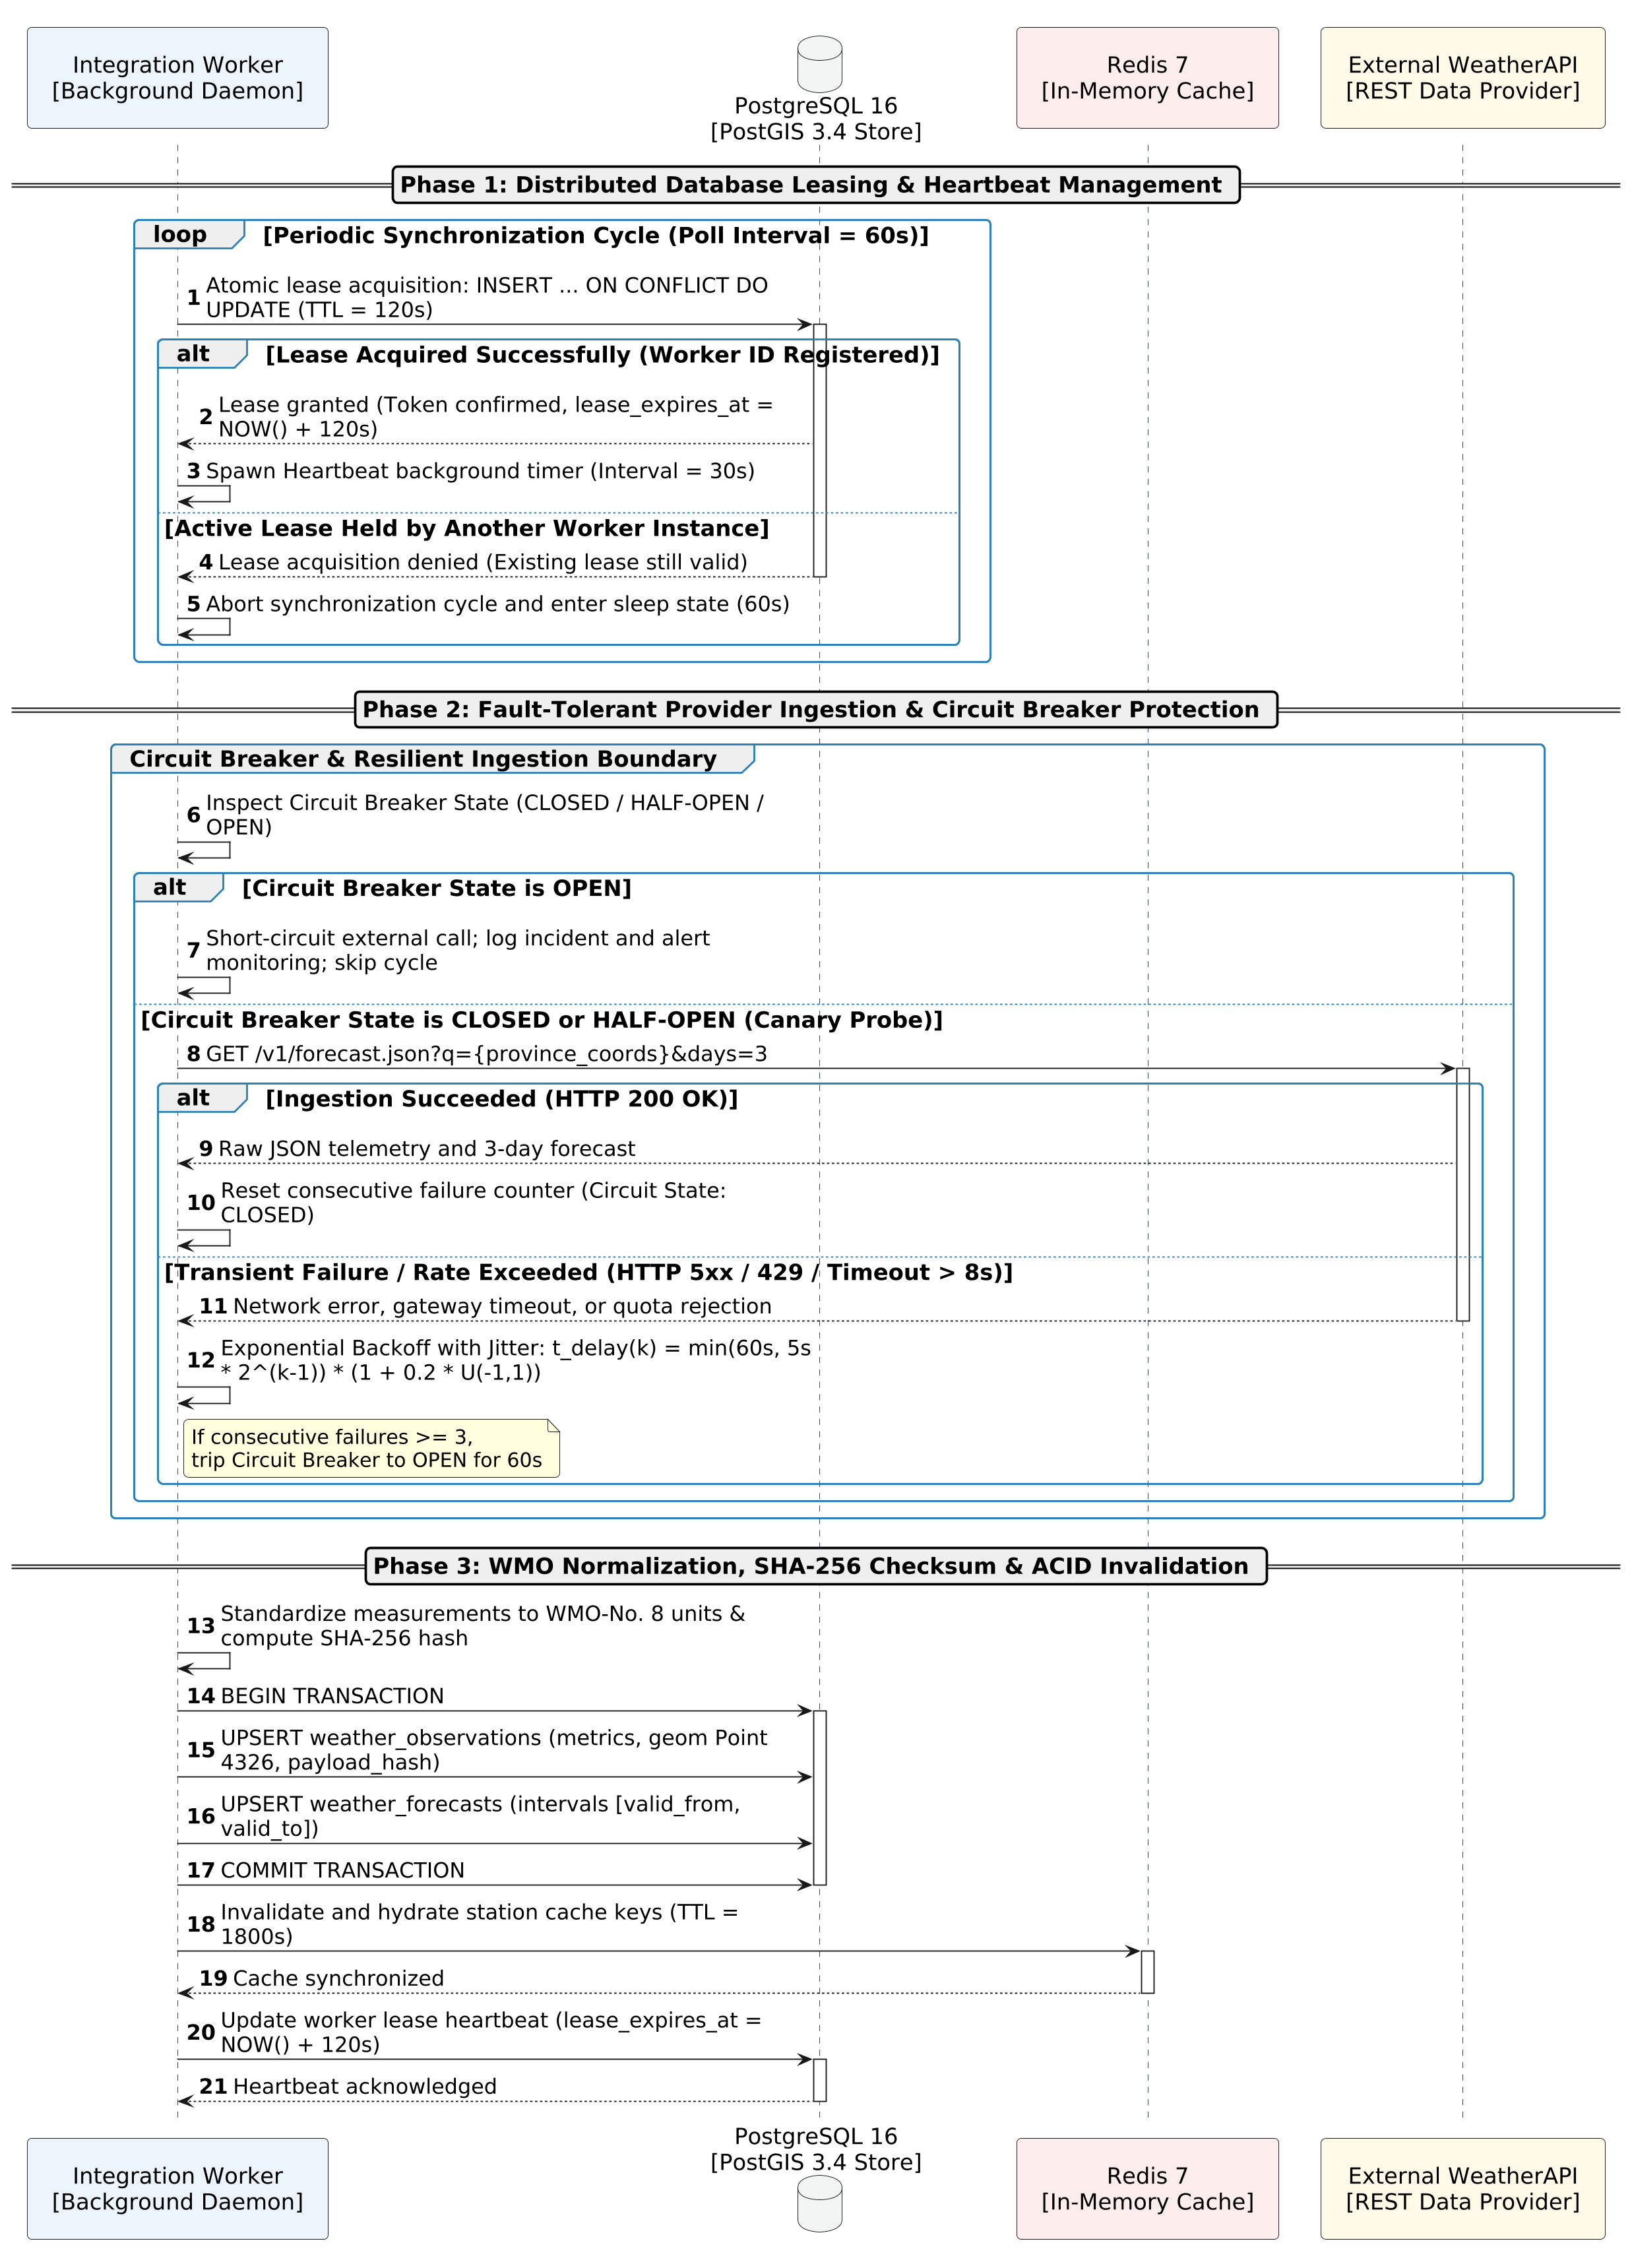
\includegraphics[width=0.92\textwidth, height=0.80\textheight, keepaspectratio]{figures/seq_ingestion.png}
\caption[Biểu đồ tuần tự đồng bộ dữ liệu thời tiết nền (ADR-001)]{Biểu đồ tuần tự quy trình đồng bộ dữ liệu khí tượng nền, cơ chế chiếm khóa phân tán và ngắt mạch tự động (ADR-001).}
\label{fig:seq_ingestion_vi}
\end{figure}

Flow hoạt động của tiến trình xử lý nền Integration Worker được phân rã thành ba giai đoạn vận hành then chốt:
\begin{itemize}
    \item[-] \textit{Pha 1: Chiếm khóa phân tán và quản trị nhịp tim (Distributed Database Leasing \& Heartbeat)}:
    Định kỳ mỗi 60 giây (chu kỳ thăm dò), worker phát câu lệnh kiểm tra và chiếm quyền độc quyền có thời hạn trên bảng \texttt{weather\_worker\_leases} của PostgreSQL thông qua lệnh nguyên tử \texttt{INSERT ... ON CONFLICT DO UPDATE WHERE lease\_expires\_at < NOW()}. Thao tác này bảo đảm chỉ duy nhất một tiến trình worker nắm giữ quyền thu thập dữ liệu trong cụm phân tán tại một thời điểm. Nếu chiếm khóa thành công (thời hạn giữ khóa $120.000\text{ ms}$), worker khởi tạo một bộ định thời nhịp tim (\texttt{heartbeat}) chạy ngầm với chu kỳ 30 giây để định kỳ cập nhật mốc thời gian hết hạn (\texttt{lease\_expires\_at} $= \text{NOW}() + 120\text{s}$). Ngược lại, nếu một tiến trình khác đang giữ khóa hợp lệ, yêu cầu bị từ chối và worker lập tức chuyển sang trạng thái ngủ trong 60 giây tiếp theo mà không gây xung đột tài nguyên.
    \item[-] \textit{Pha 2: Thu thập dữ liệu chịu lỗi và cơ chế ngắt mạch (Fault-Tolerant Provider Ingestion \& Circuit Breaker)}:
    Trước khi phát yêu cầu mạng tải dữ liệu 63 tỉnh thành, worker kiểm tra trạng thái của bộ ngắt mạch nội tại. Nếu mạch đang ở trạng thái Mở (\texttt{OPEN}), worker ngắn mạch ngay lập tức (short-circuit), hủy toàn bộ các cuộc gọi ra ngoài, ghi nhật ký cảnh báo và bỏ qua chu kỳ tải hiện tại. Nếu mạch ở trạng thái Đóng (\texttt{CLOSED}) hoặc Bán Mở (\texttt{HALF-OPEN}), worker gửi yêu cầu \texttt{GET /v1/forecast.json?q=\{province\_coords\}\&days=3} tới WeatherAPI. Khi nhận mã phản hồi HTTP 200 OK thành công, worker đặt lại bộ đếm lỗi liên tiếp về $0$. Trong trường hợp xảy ra lỗi nhất thời (mã lỗi HTTP 5xx, lỗi quá tải hạn ngạch HTTP 429 hoặc vượt quá thời gian chờ 8 giây), worker tính toán thời gian trì hoãn thử lại theo hàm số mũ kết hợp độ trễ ngẫu nhiên $t_{\text{delay}}(k)$ (Công thức~\eqref{eq:backoff_jitter}). Khi số lần thất bại liên tiếp đạt ngưỡng 3 lần, bộ ngắt mạch chuyển sang trạng thái \texttt{OPEN} trong 60 giây để bảo vệ hạn ngạch và tránh làm tê liệt dịch vụ đối tác.
    \item[-] \textit{Pha 3: Chuẩn hóa WMO, kiểm tra mã băm SHA-256 và giao dịch ACID (WMO Normalization, SHA-256 Checksum \& ACID Invalidation)}:
    Dữ liệu JSON thô nhận từ WeatherAPI được chuẩn hóa theo quy chuẩn khí tượng WMO-No. 8 (quy đổi nhiệt độ về độ C, tốc độ gió về mét/giây, lượng mưa về milimét). Worker sinh mã băm kiểm tra SHA-256 trên chuỗi dữ liệu chuẩn hóa để phát hiện các bản ghi trùng lặp nội dung. Tiếp theo, worker mở một khối giao dịch cơ sở dữ liệu (\texttt{BEGIN TRANSACTION}) và thực thi các câu lệnh \texttt{UPSERT} vào bảng \texttt{weather\_observations} (chứa các chỉ số quan trắc bề mặt kèm tọa độ hình học điểm \texttt{Point 4326}) và bảng \texttt{weather\_forecasts} (lưu trữ dự báo theo các khoảng thời gian hiệu lực), rồi xác nhận giao dịch (\texttt{COMMIT TRANSACTION}). Sau khi ghi dữ liệu bền vững thành công, worker phát tín hiệu làm mới và vô hiệu hóa bộ đệm Redis (\texttt{TTL = 1800s}) để các API phục vụ người dùng luôn đọc được dữ liệu mới nhất, đồng thời gửi tín hiệu nhịp tim cập nhật mốc thời gian khóa phân tán trong cơ sở dữ liệu.
\end{itemize}

\section{Mô hình Cơ sở Dữ liệu Không gian PostGIS và Lược đồ Thực thể (ERD)}
\label{sec:postgis_erd_schema}

\subsection{Cấu trúc Lược đồ Cơ sở Dữ liệu Phân tầng}
Cơ sở dữ liệu của hệ thống VietForecast được triển khai trên nền tảng PostgreSQL 16 tích hợp phần mở rộng không gian PostGIS 3.4. Lược đồ cơ sở dữ liệu được phân chia thành các nhóm miền dữ liệu chặt chẽ nhằm bảo đảm tính toàn vẹn tham chiếu và dễ dàng bảo trì:
\begin{itemize}
    \item[-] \textit{Nhóm an ninh phiên} (\texttt{app\_security}): Gồm bảng \texttt{app\_security.}\allowbreak\texttt{sessions} lưu trữ bản mã hóa AES-256-GCM của JWT, thẻ xác thực, thời điểm hết hạn và trạng thái thu hồi; bảng \texttt{app\_security.audit\_events} ghi nhận nhật ký bất biến về mọi hành vi truy cập nhạy cảm phục vụ kiểm toán an ninh.
    \item[-] \textit{Nhóm đơn vị hành chính và địa điểm} (\texttt{administrative}): Gồm bảng \texttt{administrative\_}\allowbreak\texttt{units} mô tả cấu trúc cây phân cấp hành chính lãnh thổ Việt Nam (Quốc gia $\rightarrow$ 63 Tỉnh/Thành phố $\rightarrow$ Quận/Huyện $\rightarrow$ Phường/Xã) kèm trường hình học \texttt{MultiPolygon}; bảng \texttt{locations} lưu trữ danh mục các điểm quan trắc, danh lam thắng cảnh và nút giao thông trọng yếu kèm tọa độ điểm \texttt{geometry(Point, 4326)}.
    \item[-] \textit{Nhóm dữ liệu khí tượng} (\texttt{weather}): Gồm bảng \texttt{weather\_providers} quản lý danh mục nhà cung cấp dữ liệu; bảng \texttt{weather\_observations} lưu trữ chuỗi thời gian các thông số quan trắc bề mặt thực nghiệm (nhiệt độ, lượng mưa, tốc độ gió, gió giật, tầm nhìn, mã WMO, giá trị băm kiểm tra SHA-256); bảng \texttt{weather\_forecasts} lưu trữ dự báo thời tiết theo các khoảng hiệu lực $[t_{\text{start}}, t_{\text{end}}]$; và bảng \texttt{weather\_worker\_leases} điều phối khóa phân tán.
    \item[-] \textit{Nhóm quy tắc rủi ro và đánh giá lộ trình} (\texttt{risk\_route}): Gồm các bảng \texttt{risk\_}\allowbreak\texttt{rule\_}\allowbreak\texttt{sets} và \texttt{risk\_}\allowbreak\texttt{rules} lưu trữ các ngưỡng tham số khí tượng theo từng loại phương tiện dưới cơ chế quản trị đa cấp (Maker-Checker); bảng \texttt{risk\_}\allowbreak\texttt{assessments} và \texttt{risk\_}\allowbreak\texttt{assessment\_}\allowbreak\texttt{evidence} lưu vết kết quả đánh giá cùng bằng chứng quan trắc phục vụ kiểm toán; các bảng \texttt{route\_}\allowbreak\texttt{requests}, \texttt{route\_}\allowbreak\texttt{options} và \texttt{route\_}\allowbreak\texttt{samples} lưu trữ yêu cầu tìm đường, hình học đa tuyến LineString của các lộ trình thay thế và các điểm lấy mẫu không-thời gian dọc tuyến.
\end{itemize}

\subsection{Tối ưu hóa Truy vấn Không gian với Cây Chỉ mục GiST}
Trong bài toán đánh giá rủi ro tuyến đường, hệ thống cần truy vấn toàn bộ các trạm thời tiết nằm trong hành lang đệm có bán kính $r_{\text{corridor}} = 15\text{ km}$ bao quanh một lộ trình di chuyển trải dài hàng trăm kilômét (tương ứng với hàng nghìn điểm tọa độ). Nếu thực hiện tính toán khoảng cách cầu phẳng trực tiếp bằng phép quét toàn bảng (Sequential Scan), độ phức tạp thuật toán sẽ đạt mức $O(M \cdot N)$ (với $M$ là số điểm lấy mẫu trên lộ trình và $N$ là tổng số trạm thời tiết), dẫn đến thời gian phản hồi kéo dài hàng giây và làm quá tải tài nguyên máy chủ.

Để giải quyết triệt để vấn đề này, PostGIS 3.4 kích hoạt cây chỉ mục tìm kiếm tổng quát GiST (Generalized Search Tree) trên toàn bộ các cột kiểu hình học \texttt{geom}. Cây chỉ mục GiST tổ chức các phần tử không gian dưới dạng cây phân cấp các hộp chữ nhật bao tối thiểu (Minimum Bounding Box -- BBOX). Động cơ cơ sở dữ liệu áp dụng quy trình lọc hai giai đoạn (Two-Tier Spatial Filtering):
\begin{itemize}
    \item[-] \textit{Giai đoạn lọc thô (Rough Pass - Bounding Box Filter)}: Hệ thống kiểm tra điều kiện giao cắt giữa hộp bao của hành lang đệm tuyến đường $G_{\text{corridor}} = \text{ST\_Buffer}(\mathcal{L}, r_{\text{corridor}})$ và hộp bao của từng điểm quan trắc:
    \begin{equation}
    \label{eq:spatial_bbox_filter_vi}
    \text{BBOX}(o.\text{geom}) \cap \text{BBOX}(G_{\text{corridor}}) \ne \emptyset
    \end{equation}
    Nhờ cấu trúc cây cân bằng của GiST, độ phức tạp của giai đoạn này chỉ là $O(\log N)$, loại bỏ hơn 95\% các trạm quan trắc nằm ngoài phạm vi tiềm năng mà không cần tính toán tọa độ chi tiết.
    \item[-] \textit{Giai đoạn lọc tinh (Exact Pass)}: Động cơ PostGIS chỉ áp dụng công thức hình học cầu trắc địa phức tạp (hàm \texttt{ST\_DWithin} trên kiểu dữ liệu \texttt{geography}) đối với tập hợp các trạm đã vượt qua giai đoạn lọc thô:
    \begin{equation}
    \label{eq:spatial_exact_filter_vi}
    d_{\text{geodetic}}(o.\text{geom}, \mathcal{L}) \le r_{\text{corridor}} \quad \text{với } \tau(o) \le 180\text{ phút}
    \end{equation}
    bảo đảm kết quả chính xác tuyệt đối theo độ cong elipxoit WGS84 với thời gian phản hồi ở mức dưới 15 mili-giây. Chi tiết thông số khai báo chỉ mục GiST và đặc tả truy vấn không gian tối ưu được trình bày trong Bảng~\ref{tab:gist_query_spec_vi} tại Chương~\ref{ch:implementation}.
\end{itemize}

\subsection{Lược đồ Thực thể Quan hệ Chuẩn hóa (ERD) và Cơ chế Quản trị Dữ liệu}
Hình~\ref{fig:erd_database_vi} biểu diễn lược đồ quan hệ thực thể (Entity-Relationship Diagram -- ERD) giữa các bảng dữ liệu then chốt trong hệ thống VietForecast, thể hiện các khóa chính, khóa ngoại và ràng buộc toàn vẹn dữ liệu.

\begin{figure}[H]
\centering
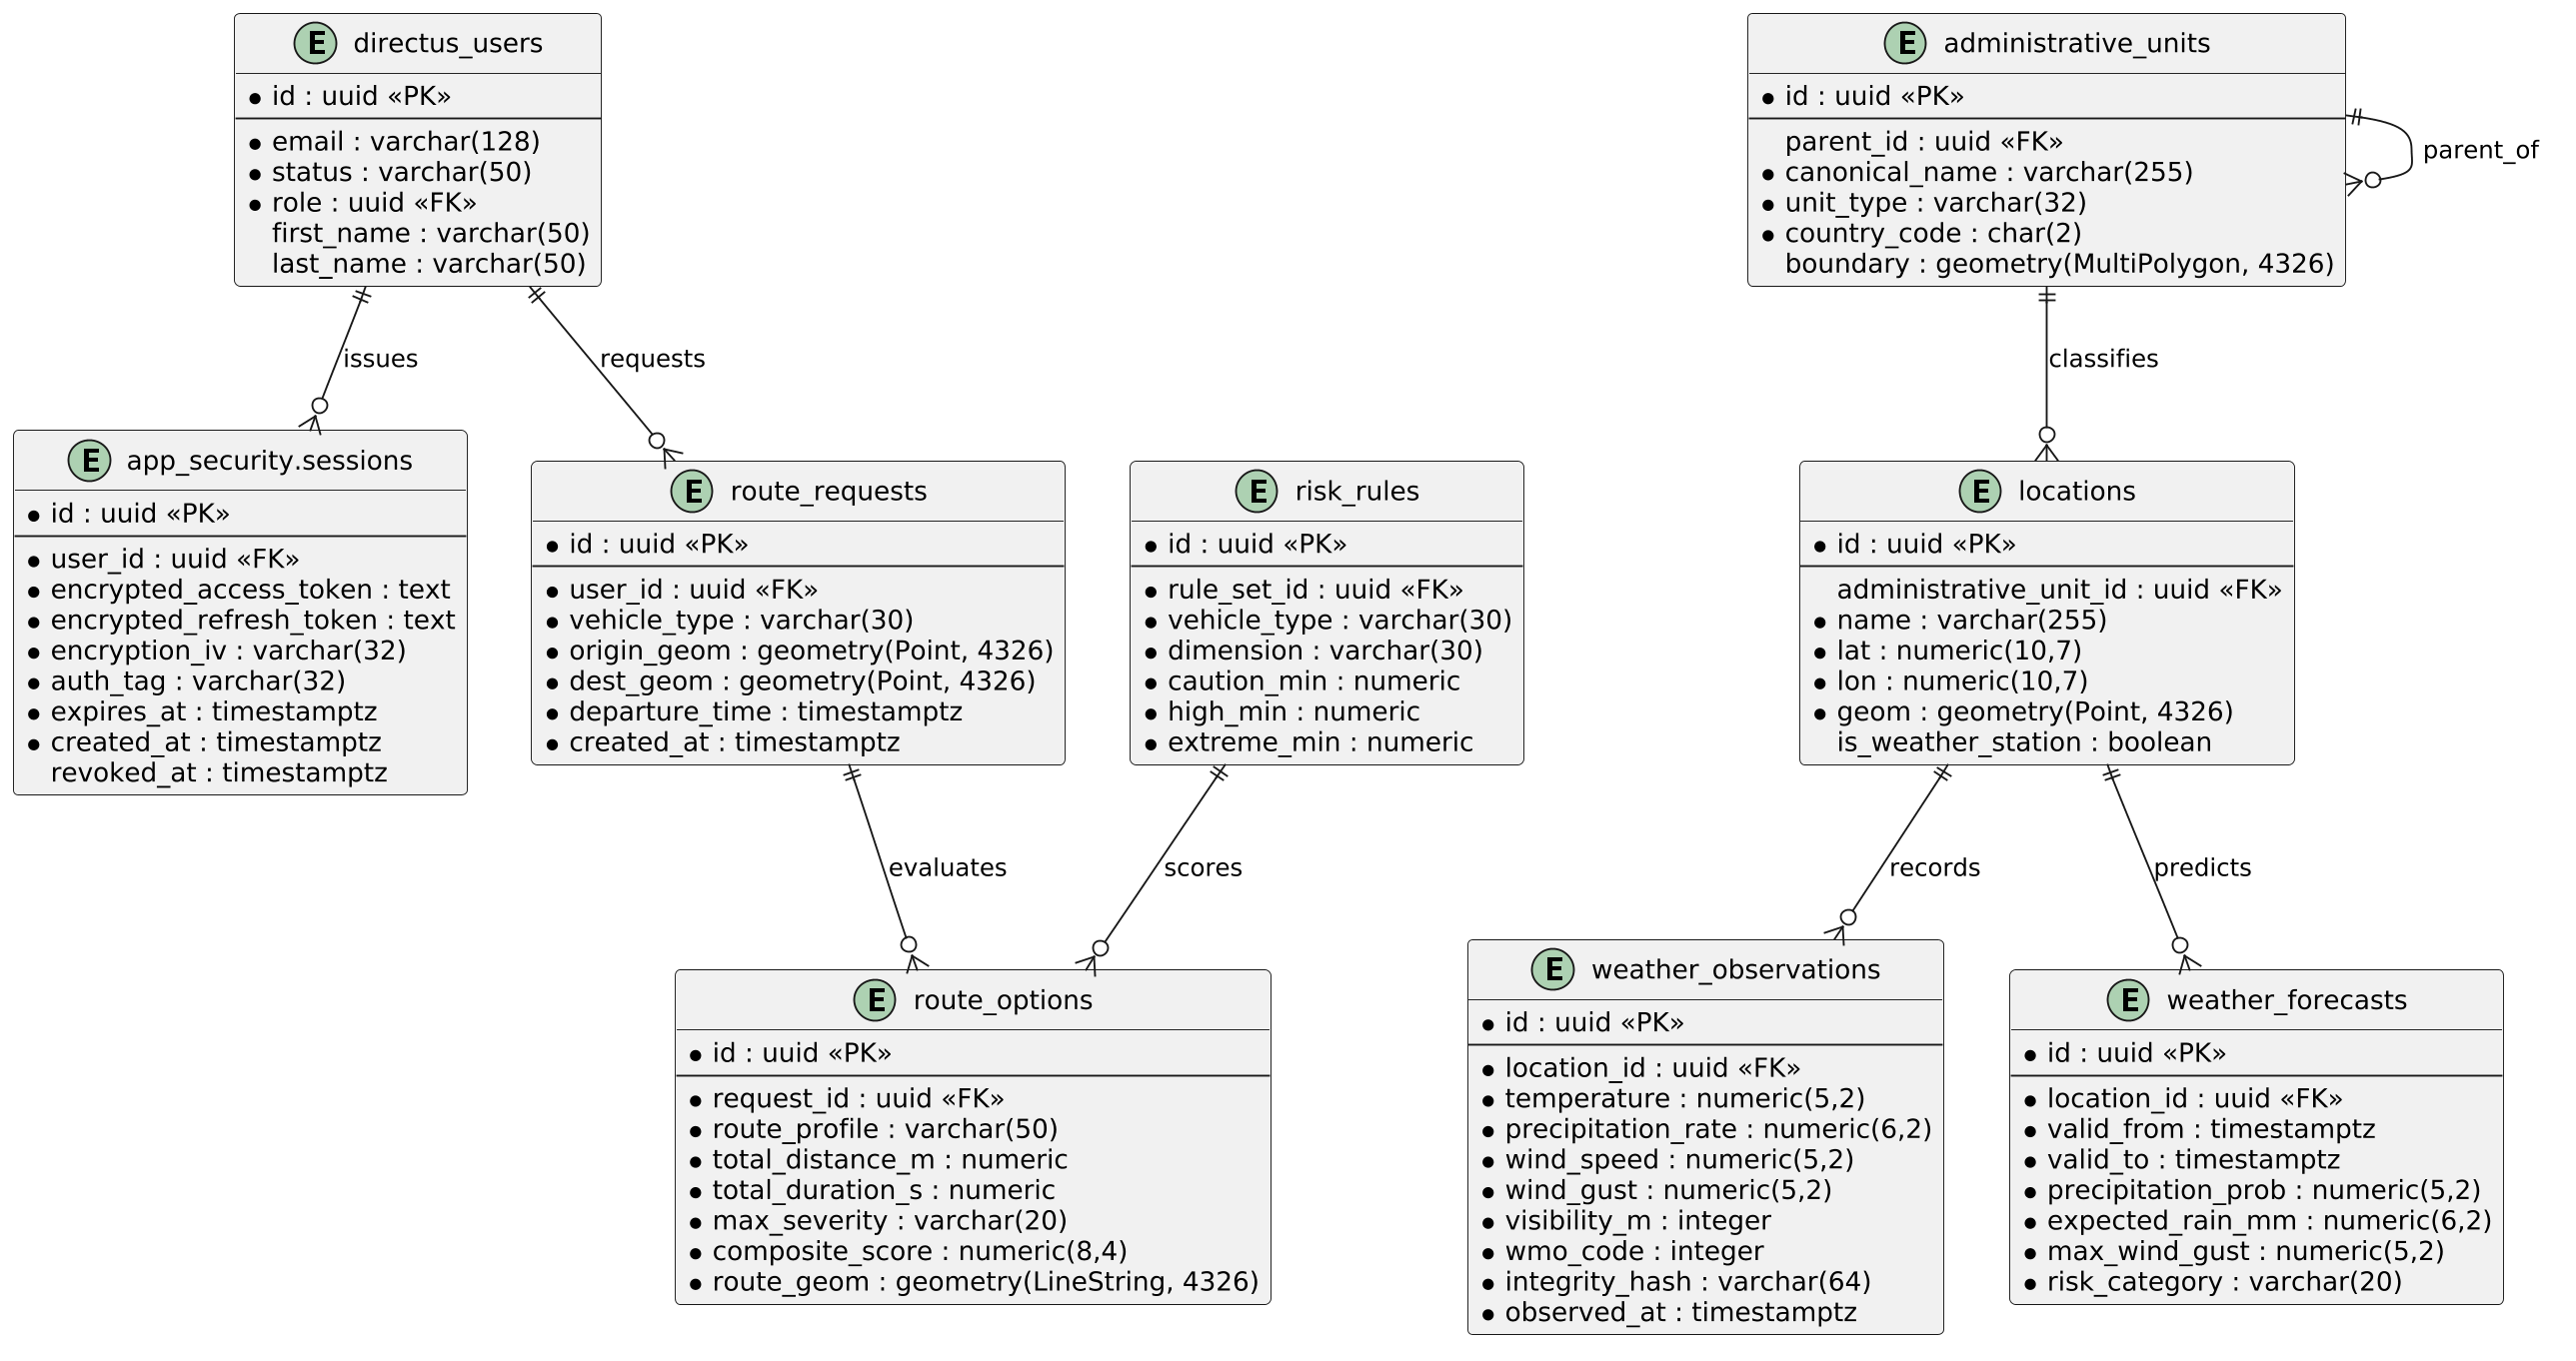
\includegraphics[width=0.95\textwidth, height=0.62\textheight, keepaspectratio]{figures/erd_database.png}
\caption[Lược đồ Thực thể Quan hệ (ERD) VietForecast]{Lược đồ Thực thể Quan hệ (ERD) mô tả cấu trúc dữ liệu không gian, an ninh danh tính và quy tắc rủi ro của VietForecast.}
\label{fig:erd_database_vi}
\end{figure}

Trong lược đồ thực thể, thực thể người dùng \texttt{directus\_}\allowbreak\texttt{users} đóng vai trò là điểm neo định danh duy nhất cho toàn bộ hệ sinh thái, vừa phát hành các phiên làm việc bảo mật trong \texttt{app\_}\allowbreak\texttt{security.}\allowbreak\texttt{sessions}, vừa liên kết với lịch sử các yêu cầu định tuyến trong \texttt{route\_}\allowbreak\texttt{requests}. Mô hình dữ liệu áp dụng hai cơ chế quản trị toàn vẹn chuyên sâu:
\begin{itemize}
    \item[-] \textit{Cơ chế kiểm soát phát hành quy tắc rủi ro (Maker-Checker Governance)}: Bộ quy tắc rủi ro trong bảng \texttt{risk\_}\allowbreak\texttt{rule\_}\allowbreak\texttt{sets} vận hành theo máy trạng thái tuần tự bao gồm các nấc: \texttt{draft}, \texttt{review}, \texttt{approved}, \texttt{published} và \texttt{retired}. Trigger cơ sở dữ liệu \texttt{app\_}\allowbreak\texttt{governance.}\allowbreak\texttt{guard\_}\allowbreak\texttt{risk\_}\allowbreak\texttt{rule\_}\allowbreak\texttt{mutation()} lập tức chặn đứng mọi hành vi chỉnh sửa hoặc xóa bỏ bản ghi con trong \texttt{risk\_}\allowbreak\texttt{rules} một khi tập quy tắc đã chuyển trạng thái rời khỏi \texttt{draft}, bảo đảm tính tất định và bất biến của các phán quyết rủi ro trong quá khứ.
    \item[-] \textit{Nhật ký kiểm toán an ninh bất biến (Immutable Audit Trail)}: Toàn bộ các thao tác nhạy cảm liên quan đến danh tính, phân quyền và điều chỉnh ngưỡng khí tượng đều kích hoạt ghi nhận vào bảng nhật ký kiểm toán \texttt{app\_}\allowbreak\texttt{security.}\allowbreak\texttt{audit\_}\allowbreak\texttt{events}. Quyền ghi nhật ký được cấp tự động thông qua hàm trigger chạy với quyền hạn bảo mật (\texttt{SECURITY DEFINER}), ngăn chặn hoàn toàn khả năng người dùng hoặc tiến trình ứng dụng can thiệp nhằm che giấu vết tích xâm nhập.
\end{itemize}

\section{Thiết kế Động cơ Đánh giá Rủi ro và Lập Lộ trình Cân bằng Đa Mục tiêu}
\label{sec:route_risk_engine}

\subsection{Mô hình Không-Thời gian và Rời rạc hóa Hành lang Di chuyển}
Động cơ đánh giá rủi ro tuyến đường của VietForecast được thiết kế nhằm giải quyết bài toán cốt lõi: biến các dữ liệu khí tượng rời rạc từ các trạm quan trắc thành chỉ dẫn di chuyển có thể hành động được cho người điều khiển phương tiện trên đường.

Hệ thống tiếp nhận các phương án lộ trình từ dịch vụ định tuyến đường bộ (OSRM), bao gồm: tuyến nhanh nhất (Fastest), tuyến ngắn nhất (Shortest) và tuyến thay thế (Alternative), mỗi tuyến biểu diễn dưới dạng đa tuyến GeoJSON LineString kèm thông số cự ly tổng $D$ và thời gian di chuyển danh định $T$. Với từng phương án lộ trình, động cơ phân rã đa tuyến thành dãy các điểm kiểm tra $p_i = (\phi_i, \lambda_i)$ với hai ràng buộc giới hạn: khoảng cách không gian giữa hai điểm liên tiếp $\Delta s \le 5\text{ km}$ và chênh lệch thời gian tiếp cận $\Delta t \le 15\text{ phút}$, tính toán dựa trên vận tốc danh định trung bình $\bar{v} = D / T$.

Fastify API thực thi truy vấn PostGIS với hàm \texttt{ST\_DWithin} để tìm kiếm các trạm quan trắc hoặc lưới dự báo thời tiết nằm trong hành lang đệm 15 km quanh từng điểm $p_i$, gán trường khí tượng tương ứng tại mốc thời gian ước lượng $t_i$.

\subsection{Ma trận Ngưỡng Rủi ro Phân hóa Phương tiện}
Động cơ rủi ro đối chiếu các tham số khí tượng tại từng điểm $p_i$ với tập luật rủi ro sáu chiều ($R_{\text{rain}}$, $R_{\text{wind}}$, $R_{\text{temp}}$, $R_{\text{vis}}$, $R_{\text{storm}}$, $R_{\text{alert}}$). Cấp độ rủi ro tại mỗi điểm lấy mẫu $S(p_i)$ tuân theo quy tắc rủi ro bao trùm nghiêm trọng nhất (Max-Severity Aggregation):
\begin{equation}
\label{eq:max_severity_aggregation_vi}
S(p_i) = \max_{d \in \mathcal{D}} R_d(p_i, v)
\end{equation}
trong đó $\mathcal{D} = \{\text{rain}, \text{wind}, \text{temp}, \text{vis}, \text{storm}, \text{alert}\}$ là tập 6 chiều rủi ro khí tượng, $v \in \{\text{motorcycle}, \text{car}\}$ biểu thị loại phương tiện tham gia giao thông, và $R_d \in \{0, 1, 2, 3\}$ tương ứng với 4 cấp độ: \texttt{Unknown} (0), \texttt{Low} (1), \texttt{Caution} (2), và \texttt{High} (3).

Bảng~\ref{tab:vehicle_risk_matrix_vi} chi tiết hóa ma trận ngưỡng kích hoạt rủi ro phân hóa theo phương tiện theo quy chuẩn an toàn giao thông đường bộ Việt Nam.

\begin{table}[H]
\centering
\small
\caption[Ma trận ngưỡng rủi ro phân hóa theo loại phương tiện]{Ma trận ngưỡng kích hoạt rủi ro thời tiết phân hóa theo loại phương tiện (RISK-001, RISK-002).}
\label{tab:vehicle_risk_matrix_vi}
\begin{tabularx}{\textwidth}{l >{\raggedright\arraybackslash}p{2.8cm} X X}
\toprule
\textbf{Chiều rủi ro} & \textbf{Chỉ số \& Đơn vị} & \textbf{Ngưỡng Thận trọng (Caution)} & \textbf{Ngưỡng Nguy hiểm (High)} \\
\midrule
Lượng mưa ($R_{\text{rain}}$) & Cường độ mưa (mm/h) & 
Xe máy: $10 \le r < 25$ \newline Ô tô: $15 \le r < 35$ & 
Xe máy: $r \ge 25$ \newline Ô tô: $r \ge 35$ \\
\addlinespace
Gió giật ($R_{\text{wind}}$) & Vận tốc gió giật (km/h) & 
Xe máy: $25 \le w < 40$ \newline Ô tô: $45 \le w < 60$ & 
Xe máy: $w \ge 40$ \newline Ô tô: $w \ge 60$ \\
\addlinespace
Tầm nhìn ($R_{\text{vis}}$) & Tầm nhìn ngang (m) & 
Xe máy: $1.000 \le v < 2.000$ \newline Ô tô: $500 \le v < 1.000$ & 
Xe máy: $v < 1.000$ \newline Ô tô: $v < 500$ \\
\addlinespace
Nhiệt độ ($R_{\text{temp}}$) & Nhiệt độ bề mặt ($^\circ\text{C}$) & 
Xe máy: $36$--$38^\circ\text{C}$ hoặc $10$--$13^\circ\text{C}$ \newline Ô tô: $38$--$40^\circ\text{C}$ hoặc $5$--$8^\circ\text{C}$ & 
Xe máy: $> 38^\circ\text{C}$ hoặc $< 10^\circ\text{C}$ \newline Ô tô: $> 40^\circ\text{C}$ hoặc $< 5^\circ\text{C}$ \\
\addlinespace
Dông sét ($R_{\text{storm}}$) & Hiện tượng đối lưu WMO & 
Có dông xa hoặc mây vũ tích & 
Dông sét trực tiếp hoặc mưa đá \\
\addlinespace
Cảnh báo ($R_{\text{alert}}$) & Cấp thiên tai quốc gia & 
Rủi ro thiên tai Cấp 1--2 & 
Rủi ro thiên tai Cấp 3 trở lên \\
\bottomrule
\end{tabularx}
\end{table}

\subsection{Hàm Mục tiêu Tối ưu hóa Cân bằng Tuyến đường}
Hệ thống tính toán điểm số tổng hợp cho từng phương án lộ trình dựa trên công thức hàm mục tiêu chuẩn hóa:
\begin{equation}
\label{eq:route_balanced_score_vi}
Score_{\text{balanced}} = w_{\text{risk}} \cdot \hat{S}_{\text{route}} + w_{\text{time}} \cdot \hat{T} + w_{\text{dist}} \cdot \hat{D}
\end{equation}
với bộ trọng số mặc định $w_{\text{risk}} = 0{,}5$, $w_{\text{time}} = 0{,}3$, $w_{\text{dist}} = 0{,}2$. Điểm rủi ro trung bình dọc tuyến $\hat{S}_{\text{route}} = \frac{1}{K} \sum_{k=1}^K S(p_k) / 3$, cự ly $\hat{D} = D / \max(D)$ và thời gian $\hat{T} = T / \max(T)$ được chuẩn hóa về miền $[0, 1]$. Tuyến đường có điểm số thấp nhất sẽ được gắn nhãn Khuyến nghị an toàn (Weather-Safer Recommended), giúp người lái xe cân bằng tối ưu giữa thời gian hành trình và sự an toàn tính mạng trước các hình thái thời tiết cực đoan.

\subsection{Quy trình Đánh giá Rủi ro Lộ trình và Biểu đồ Tuần tự}
Hình~\ref{fig:seq_route_risk_vi} mô tả chi tiết biểu đồ tuần tự toàn diện của luồng đánh giá rủi ro thời tiết lộ trình đa phương án từ khi người dùng phát lệnh tìm đường trên giao diện MapLibre GL.

\begin{figure}[H]
\centering
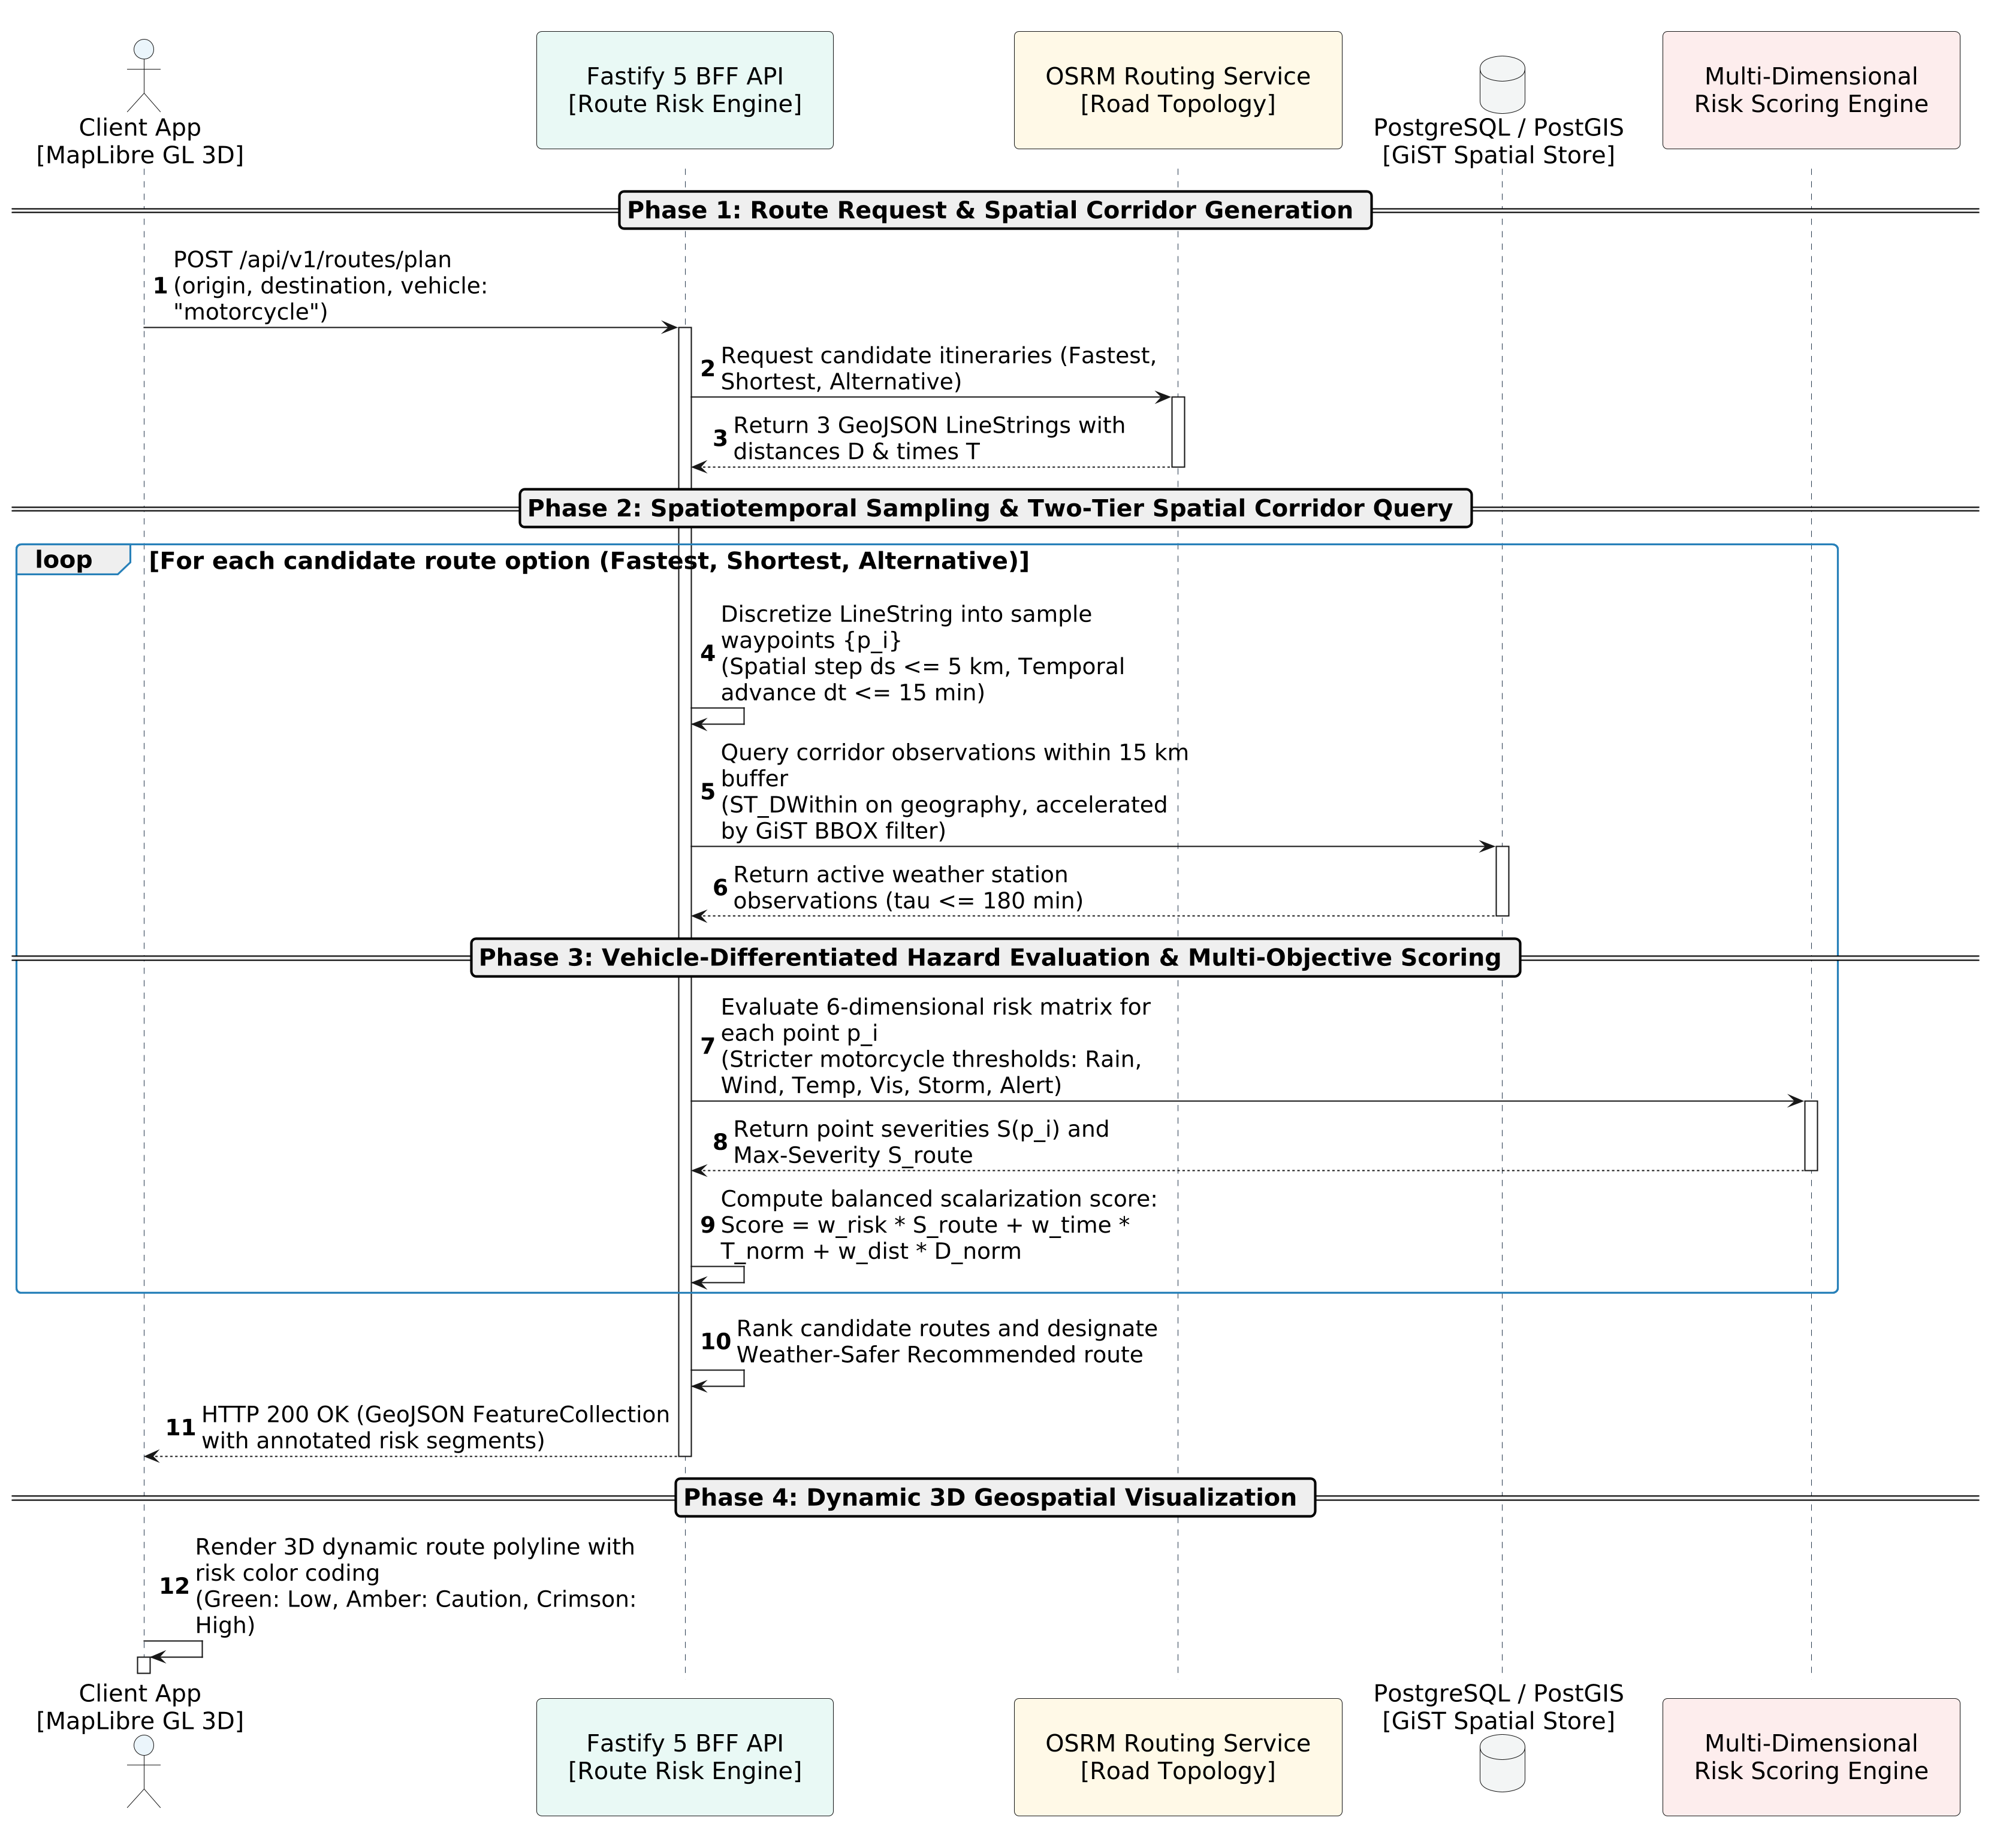
\includegraphics[width=0.95\textwidth, keepaspectratio]{figures/seq_route_risk.png}
\caption[Biểu đồ tuần tự đánh giá rủi ro thời tiết lộ trình]{Biểu đồ tuần tự quy trình đánh giá rủi ro thời tiết lộ trình đa mục tiêu, lấy mẫu không-thời gian và trực quan hóa bản đồ 3D.}
\label{fig:seq_route_risk_vi}
\end{figure}

Flow hoạt động của quy trình đánh giá rủi ro lộ trình bao gồm bốn pha chính xác như sau:
\begin{itemize}
    \item[-] \textit{Pha 1: Tiếp nhận yêu cầu tìm đường và khai phá lộ trình ứng viên}:
    Ứng dụng khách MapLibre GL gửi yêu cầu \texttt{POST /api/v1/routes/plan} kèm tọa độ điểm xuất phát, điểm đến và loại phương tiện (\texttt{motorcycle} hoặc \texttt{car}) tới Fastify API. Fastify chuyển tiếp yêu cầu tới dịch vụ định tuyến đường bộ OSRM để thu nhận ba phương án lộ trình độc lập: tuyến nhanh nhất (Fastest), tuyến ngắn nhất (Shortest) và tuyến thay thế (Alternative). Mỗi tuyến được định nghĩa dưới dạng đa tuyến hình học GeoJSON LineString kèm các thông số cự ly tổng $D$ và thời gian di chuyển danh định $T$.
    \item[-] \textit{Pha 2: Rời rạc hóa không-thời gian và truy vấn trắc địa hành lang đệm}:
    Với từng phương án lộ trình, động cơ phân rã đa tuyến LineString thành dãy các điểm kiểm tra $p_i = (\phi_i, \lambda_i)$ với hai ràng buộc giới hạn: khoảng cách không gian giữa hai điểm liên tiếp $\Delta s \le 5\text{ km}$ và chênh lệch thời gian tiếp cận $\Delta t \le 15\text{ phút}$ (tính dựa trên vận tốc danh định trung bình $\bar{v} = D / T$).
    Tại từng điểm kiểm tra $p_i$, Fastify API thực thi truy vấn không gian trắc địa PostGIS thông qua hàm \texttt{ST\_DWithin}. Nhờ cây chỉ mục GiST 2D, hệ thống thực hiện phép lọc thô qua hộp bao BBOX với độ phức tạp chỉ $O(\log N)$, sau đó mới tính toán cự ly trắc địa elipxoit WGS84 chính xác để thu thập toàn bộ các trạm quan trắc hoặc lưới dự báo trong hành lang đệm bán kính $r_{\text{corridor}} = 15\text{ km}$ có độ tươi mới dữ liệu $\tau \le 180\text{ phút}$.
    \item[-] \textit{Pha 3: Đánh giá ma trận rủi ro phân hóa phương tiện và chấm điểm đa mục tiêu}:
    Động cơ đối chiếu các thông số quan trắc khí tượng thu nhận được tại từng điểm $p_i$ với tập luật rủi ro sáu chiều: Lượng mưa ($R_{\text{rain}}$), Gió giật ($R_{\text{wind}}$), Nhiệt độ ($R_{\text{temp}}$), Tầm nhìn ($R_{\text{vis}}$), Dông sét ($R_{\text{storm}}$) và Cấp độ thiên tai ($R_{\text{alert}}$). Cấp độ rủi ro tại mỗi điểm $S(p_i)$ tuân theo quy tắc bao trùm nghiêm trọng nhất $S(p_i) = \max_{d \in \mathcal{D}} R_d(p_i, v)$ theo công thức~\eqref{eq:max_severity_aggregation_vi}. Đối với xe máy, các ngưỡng kích hoạt được siết chặt hơn 30\% so với ô tô nhằm phản ánh nguy cơ mất an toàn thực tế (Bảng~\ref{tab:vehicle_risk_matrix_vi}).
    Hệ thống tính toán điểm số hàm mục tiêu cân bằng $Score_{\text{balanced}}$ theo công thức~\eqref{eq:route_balanced_score_vi}, kết hợp giữa độ an toàn thời tiết dọc tuyến ($\hat{S}_{\text{route}}$), thời gian di chuyển ($\hat{T}$) và cự ly hành trình ($\hat{D}$). Tuyến đường có điểm số tổng hợp thấp nhất được xếp hạng ưu tiên và gắn nhãn Khuyến nghị an toàn (Weather-Safer Recommended).
    \item[-] \textit{Pha 4: Đóng gói dữ liệu và trực quan hóa 3D động}:
    Fastify API hoàn tất tính toán và trả về phản hồi HTTP 200 OK dưới dạng gói GeoJSON FeatureCollection chứa các đa tuyến lộ trình đã phân đoạn và gắn mã màu rủi ro tương ứng: xanh lục (\texttt{Low}), vàng cam (\texttt{Caution}) và đỏ thẫm (\texttt{High}). Ứng dụng giao diện MapLibre GL 4 tận dụng khả năng tăng tốc phần cứng WebGL để dựng mô hình địa hình ba chiều (3D terrain), hiển thị đa tuyến lộ trình động và cho phép người lái xe trực tiếp theo dõi các phân đoạn nguy hiểm dọc hành trình.
\end{itemize}

\section{Thiết kế Trợ lý AI Khí tượng Đàm thoại có Kiểm chứng Dữ liệu}
\label{sec:grounded_ai_assistant}

\subsection{Kiến trúc Điều phối Công cụ Đàm thoại (Tool Orchestration)}
Để đáp ứng nhu cầu giao tiếp đàm thoại tự nhiên của người dùng mà vẫn kiểm soát và giảm thiểu tối đa hiện tượng ảo giác (hallucination) thường gặp ở các mô hình ngôn ngữ lớn, VietForecast thiết kế kiến trúc Trợ lý AI có kiểm chứng dữ liệu thực nghiệm (Grounded AI Engine) dựa trên mô hình nền tảng Google Gemini 1.5 Flash.

Google Gemini 1.5 Flash được cấu hình đóng vai trò là bộ phân tích ngôn ngữ tự nhiên và điều phối công cụ (Tool Orchestrator). Mô hình hoàn toàn không được phép tự do tạo sinh các thông số khí tượng giả lập. Hệ thống trang bị cho Gemini năm công cụ gọi hàm chuẩn hóa:
\begin{itemize}
    \item[-] \texttt{search\_location}: Tra cứu tọa độ, đơn vị hành chính và địa danh từ cơ sở dữ liệu chuẩn hóa 63 tỉnh thành.
    \item[-] \texttt{get\_current\_weather}: Trích xuất các thông số quan trắc khí tượng bề mặt mới nhất tại trạm đo tương ứng.
    \item[-] \texttt{get\_forecast}: Lấy chuỗi dữ liệu dự báo khí quyển theo từng khoảng hiệu lực thời gian.
    \item[-] \texttt{assess\_travel\_risk}: Tính toán cấp độ rủi ro tại một địa điểm cụ thể dựa trên ma trận ngưỡng phương tiện.
    \item[-] \texttt{evaluate\_route}: Đánh giá an toàn lộ trình qua hàm ánh xạ:
    \begin{equation}
    \label{eq:tool_evaluate_route_vi}
    \mathcal{F}_{\text{route}}: (\text{origin}, \text{destination}, \text{vehicleType}) \longrightarrow \text{RouteRiskAssessment}
    \end{equation}
    Khai báo đặc tả tham số chi tiết của công cụ gọi hàm \texttt{evaluate\_route} được trình bày trong Bảng~\ref{tab:gemini_tool_schema_vi} tại Chương~\ref{ch:implementation}.
\end{itemize}

\subsection{Cơ chế Kiểm chứng Dữ liệu và Trích dẫn Thực nghiệm (Grounded Evidence Pipeline)}
Chu trình kiểm chứng dữ liệu thực nghiệm vận hành theo ba bước nghiêm ngặt:
\begin{itemize}
    \item[-] \textit{Tiếp nhận và gọi công cụ}: Khi nhận diện câu hỏi từ người dùng (ví dụ: \textit{"Chiều nay tôi đi xe máy từ Hà Nội về Ninh Bình có an toàn không?"}), Gemini sinh cấu trúc gọi công cụ \texttt{evaluate\_route}. Fastify API đón bắt lệnh gọi, thực thi truy vấn PostGIS và dịch vụ định tuyến, kiểm tra độ tươi mới $\tau \le 180\text{ phút}$, rồi đóng gói dữ liệu quan trắc thực tế gửi ngược lại mô hình.
    \item[-] \textit{Tổng hợp câu trả lời kèm bằng chứng}: Gemini tổng hợp câu trả lời bằng tiếng Việt tự nhiên dựa độc quyền trên dữ liệu được cung cấp. Phản hồi bắt buộc đính kèm trích dẫn nguồn trạm đo (Station ID), mốc thời gian quan trắc và câu khuyến cáo an toàn bắt buộc.
    \item[-] \textit{Cơ chế dự phòng tất định (Deterministic Fallback Engine)}: Trong trường hợp đường truyền quốc tế gián đoạn hoặc dịch vụ Gemini vượt hạn mức, bộ điều phối \texttt{GroundedRuleEngineAdapter} tại Fastify API tự động kích hoạt. Thành phần này dùng biểu thức chính quy (regular expressions) nhận dạng thực thể vị trí và áp dụng trực tiếp cây quyết định tất định để trả về kết quả dự báo và cảnh báo rủi ro chính xác 100\% mà không làm gián đoạn trải nghiệm người dùng.
\end{itemize}

\section{Tóm tắt chương}
\label{sec:chapter3_summary}
Chương 3 đã trình bày chi tiết toàn bộ thiết kế kiến trúc hệ thống và thiết kế kỹ thuật của nền tảng VietForecast. Thông qua việc phân rã dịch vụ vi mô theo mô hình C4 Container, thiết lập phân vùng mạng Docker cách ly tuyệt đối tầng dữ liệu, xây dựng ranh giới phiên bảo mật phía máy chủ AES-256-GCM (ADR-004) triệt tiêu nguy cơ tấn công XSS, và triển khai tiến trình xử lý nền Worker tự phục hồi với cơ chế chiếm khóa phân tán (ADR-001), hệ thống đạt được sự cân bằng tối ưu giữa hiệu năng vận hành, độ tươi mới của dữ liệu và an ninh thông tin. Lược đồ cơ sở dữ liệu PostGIS 3.4 kết hợp chỉ mục không gian GiST, động cơ đánh giá rủi ro lộ trình đa mục tiêu phân hóa theo phương tiện và trợ lý AI có kiểm chứng dữ liệu tạo nên nền tảng kỹ thuật vững chắc để hệ thống vận hành tin cậy trong môi trường khí hậu nhiệt đới gió mùa phức tạp tại Việt Nam. Toàn bộ các thiết kế kiến trúc này được hiện thực hóa chi tiết trong Chương 4.

\chapter{Hiện thực hóa hệ thống}
\label{ch:implementation}

Chương này trình bày toàn diện quá trình hiện thực hóa phần mềm cho toàn bộ nền tảng VietForecast dựa trên các nguyên lý và mô hình kiến trúc đã được thiết kế tại Chương~\ref{ch:architecture}. Toàn bộ hệ thống được xây dựng theo mô hình kho mã nguồn hợp nhất (monorepo), áp dụng kiểm kiểu tĩnh nghiêm ngặt với TypeScript 5.5, đóng gói đa dịch vụ vi mô qua Docker Compose với mạng lưới ba tầng phân lập. Nội dung chương tập trung làm rõ việc lập trình tầng dịch vụ backend hiệu năng cao với Fastify 5, cơ chế phong tỏa an ninh phiên bảo mật phía máy chủ (ADR-004), tối ưu hóa truy vấn hành lang không gian hai giai đoạn với cây chỉ mục GiST trên PostGIS 3.4, tiến trình xử lý nền Worker tự phục hồi với khóa phân tán (ADR-001), động cơ đánh giá rủi ro lộ trình đa mục tiêu phân hóa theo phương tiện, trợ lý AI đàm thoại có kiểm chứng dữ liệu thực nghiệm cùng bộ chuyển đổi dự phòng tất định, giao diện bản đồ 3D WebGL tương tác thời gian thực, và quy trình bảo đảm chất lượng thông qua kiểm thử tự động trên CI/CD.

\section{Môi trường phát triển, Ngăn xếp triển khai và Kiến trúc Monorepo}
\label{sec:monorepo_deployment_stack}

\subsection{Cấu trúc Kho mã nguồn Hợp nhất Monorepo và Ràng buộc Kiểu tĩnh}
Nhằm tối ưu hóa năng suất kỹ nghệ phần mềm và loại bỏ nguy cơ phân mảnh giao diện lập trình giữa các dịch vụ phân tán, nền tảng VietForecast được tổ chức dưới dạng kho mã nguồn hợp nhất (monorepo) quản lý bởi công cụ đóng gói \texttt{pnpm workspaces}. Hệ thống thiết lập phiên bản ngôn ngữ TypeScript 5.5 ở chế độ kiểm kiểu nghiêm ngặt tuyệt đối (\texttt{strict: true}, \texttt{noImplicitAny: true}, \texttt{exactOptionalPropertyTypes: true}) và định dạng mô-đun chuẩn \texttt{NodeNext}.

Cấu trúc thư mục của monorepo được phân chia thành hai không gian độc lập:
\begin{itemize}
    \item[-] \textit{Không gian ứng dụng (\texttt{apps/})}: Chứa các tiến trình thực thi độc lập bao gồm cổng giao tiếp nghiệp vụ \texttt{apps/api}, tiến trình nền thu thập khí tượng \texttt{apps/worker}, hệ thống quản trị danh tính và nội dung \texttt{apps/directus}, và ứng dụng giao diện người dùng \texttt{apps/web}.
    \item[-] \textit{Không gian gói dùng chung (\texttt{packages/})}: Chứa các thư viện nền tảng gồm \texttt{packages/contracts} (định nghĩa toàn bộ các đối tượng truyền dữ liệu DTO, lược đồ xác thực hợp đồng Zod/Ajv, và danh mục hằng số chuẩn hóa) và \texttt{packages/config} (lưu trữ cấu hình biên dịch TypeScript và quy tắc kiểm tra tĩnh ESLint 9).
\end{itemize}

Việc tập trung toàn bộ định nghĩa giao tiếp vào gói \texttt{packages/contracts} bảo đảm tính nhất quán xuyên suốt: bất kỳ thay đổi nào về cấu trúc dữ liệu thời tiết, mã rủi ro hoặc tham số định tuyến đều được trình biên dịch TypeScript xác thực tĩnh tức thời ở cả máy khách lẫn máy chủ, triệt tiêu hoàn toàn các lỗi sai lệch kiểu dữ liệu tại thời điểm chạy (\textit{runtime type errors}).

\subsection{Phân vùng Mạng Ba tầng và Triển khai Container Hóa}
Toàn bộ hệ sinh thái VietForecast được đóng gói thành các vùng chứa container tiêu chuẩn thông qua tệp khai báo cấu trúc \texttt{compose.yaml}. Hạ tầng vận hành được phân vùng thành ba mạng ảo nội bộ nhằm thực thi nguyên lý đặc quyền tối thiểu ở cấp độ giao vận mạng:
\begin{itemize}
    \item[-] \textit{Tầng biên và Cổng đảo ngược (\texttt{vnwa\_edge\_net})}: Tiếp nhận lưu lượng trực tiếp từ Internet công cộng qua các cổng tiêu chuẩn 80 (HTTP) và 443 (HTTPS) thông qua Nginx Reverse Proxy. Nginx đảm nhiệm chấm dứt phiên mã hóa TLS, thiết lập các tiêu đề an ninh nghiêm ngặt, và phân phối lưu lượng tới các cổng nội bộ của ứng dụng web và API.
    \item[-] \textit{Tầng ứng dụng và Điều phối nghiệp vụ (\texttt{vnwa\_app\_net})}: Chứa các vùng chứa \texttt{apps/api}, \texttt{apps/worker} và \texttt{apps/directus}. Các dịch vụ này được cấp quyền giao tiếp với nhau và kết nối tới cơ sở dữ liệu để thực thi nghiệp vụ, đồng thời có thể gửi yêu cầu ra mạng ngoài để tương tác với các API khí tượng và dịch vụ đám mây.
    \item[-] \textit{Tầng dữ liệu cô lập tuyệt đối (\texttt{vnwa\_data\_net})}: Chứa cơ sở dữ liệu không gian PostgreSQL 16 (tích hợp PostGIS 3.4) và bộ đệm trong bộ nhớ Redis 7. Mạng này được cấu hình với thuộc tính cô lập đặc biệt \texttt{internal: true}, ngắt hoàn toàn cổng định tuyến Internet (Default Gateway). Do đó, các vùng chứa dữ liệu không thể bị truy cập trực tiếp từ bên ngoài và cũng không thể gửi dữ liệu trái phép ra Internet trong trường hợp bị xâm nhập.
\end{itemize}

Các container được trang bị cơ chế kiểm tra sức khỏe tự động (\textit{healthchecks}) định kỳ 10 giây sử dụng các công cụ chuyên dụng như \texttt{pg\_isready} cho PostgreSQL, \texttt{redis-cli ping} cho Redis, và các điểm cuối kiểm tra trạng thái \texttt{/health} và \texttt{/ready} cho Fastify API và Integration Worker, bảo đảm việc khởi động và phục hồi diễn ra hoàn toàn tự động theo đúng thứ tự phụ thuộc.

\section{Hiện thực Tầng Dịch vụ Backend và Ranh giới Bảo mật Phiên (ADR-004)}
\label{sec:backend_fastify_impl}

\subsection{Vòng đời Xử lý Yêu cầu và Chuỗi Hook của Fastify 5}
Tầng dịch vụ backend \texttt{apps/api} được hiện thực hóa dựa trên Fastify 5, tận dụng kiến trúc bất đồng bộ hướng sự kiện và trình phân giải chuỗi JSON siêu tốc \texttt{fast-json-stringify}. Để bảo đảm tính nhất quán trong việc kiểm soát truy cập và bảo vệ tài nguyên, mọi yêu cầu HTTP gửi đến API đều phải đi qua chuỗi móc nối vòng đời (\textit{lifecycle hooks}) được thiết lập nghiêm ngặt:
\begin{itemize}
    \item[-] \textit{Giai đoạn tiếp nhận (\texttt{onRequest})}: Kích hoạt bộ kiểm soát tần suất phân tán Token Bucket dựa trên Redis 7. Hệ thống giải mã địa chỉ IP máy khách và giá trị băm của thẻ nhận dạng phiên; nếu lưu lượng vượt quá hạn mức cho phép, Fastify lập tức phản hồi mã trạng thái HTTP 429 (\textit{Too Many Requests}) kèm tiêu đề \texttt{Retry-After} mà không chuyển tiếp vào tầng nghiệp vụ nặng.
    \item[-] \textit{Giai đoạn xác thực cấu trúc (\texttt{preValidation})}: Sử dụng trình biên dịch lược đồ Ajv để kiểm tra định dạng dữ liệu đầu vào (phương thức, tiêu đề, tham số đường dẫn và thân yêu cầu JSON) dựa trên các hợp đồng chia sẻ từ \texttt{packages/contracts}. Các trường dữ liệu độc hại hoặc không đúng quy chuẩn lập tức bị loại bỏ với mã lỗi HTTP 400 (\textit{Bad Request}).
    \item[-] \textit{Giai đoạn kiểm tra an ninh phiên (\texttt{preHandler})}: Trích xuất thẻ đục mờ ngẫu nhiên từ cookie an toàn \texttt{\_\_Host-vnwa\_session}. Hook thực hiện băm SHA-256 thẻ nhận dạng, truy vấn bảng lưu trữ \texttt{app\_security.sessions}, đối chiếu trạng thái thu hồi và thời gian sống, thực thi xoay vòng phiên trượt ngầm nếu thời hạn token sắp hết, và gắn đối tượng định danh người dùng (\texttt{userId}, \texttt{roleId}) vào ngữ cảnh thực thi của tuyến dịch vụ.
    \item[-] \textit{Giai đoạn hậu xử lý và kiểm toán (\texttt{onResponse})}: Tự động đo lường độ trễ xử lý chính xác ở mức micro-giây phục vụ hệ thống giám sát Prometheus, đồng thời kích hoạt ghi nhận sự kiện an ninh vào bảng nhật ký kiểm toán \texttt{app\_security.audit\_events} đối với các thao tác nhạy cảm.
\end{itemize}

\subsection{Hiện thực Bao bì Mã hóa Khí quyển và Bảo vệ Chống Sai biệt Thời gian}
Mô-đun an ninh mật mã học được tập trung tại tệp \texttt{apps/api/src/crypto.ts}, cung cấp các hàm nghiệp vụ mật mã vững chắc được xây dựng trực tiếp trên thư viện chuẩn \texttt{node:crypto}:
\begin{itemize}
    \item[-] \textit{Bao bì mã hóa đối xứng AES-256-GCM}: Được sử dụng để mã hóa toàn bộ mã truy cập (\texttt{access\_token}) và mã làm mới (\texttt{refresh\_token}) của Directus trước khi ghi vào cơ sở dữ liệu. Hàm \texttt{encryptSecret} khởi tạo một vectơ khởi tạo ngẫu nhiên (IV) độ dài 96 bit (12 byte) từ nguồn ngẫu nhiên an toàn mật mã CSPRNG (\texttt{randomBytes(12)}), thực thi mã hóa khối với khóa bí mật 256 bit \texttt{API\_SESSION\_ENCRYPTION\_KEY}, và trích xuất thẻ xác thực toàn vẹn 128 bit (\texttt{authTag}). Kết quả mã hóa được đóng gói tuần tự thành chuỗi ký tự theo quy chuẩn:
    \begin{equation}
    \label{eq:crypto_envelope_vi}
    \text{Envelope} = \text{"v1"} \,.\, \text{Base64URL}(\text{IV}) \,.\, \text{Base64URL}(\text{Tag}) \,.\, \text{Base64URL}(\text{Ciphertext})
    \end{equation}
    Khi giải mã thông qua hàm \texttt{decryptSecret}, hệ thống kiểm tra chặt chẽ tiền tố phiên bản \texttt{v1} và xác thực tính toàn vẹn của dữ liệu thông qua thẻ \texttt{authTag}; nếu có bất kỳ sự can thiệp trái phép nào vào dữ liệu nhị phân, giải thuật ném ngoại lệ lập tức và hủy bỏ phiên xử lý.
    \item[-] \textit{Sinh thẻ đục mờ và băm một chiều an toàn}: Hàm \texttt{createOpaqueToken(32)} thu nhận 32 byte ngẫu nhiên chất lượng cao từ CSPRNG và mã hóa thành chuỗi 43 ký tự an toàn URL (\texttt{base64url}) để cấp phát cho cookie của người dùng. Trước khi ghi nhận vào hệ quản trị cơ sở dữ liệu, thẻ được băm một chiều bằng giải thuật SHA-256 qua hàm \texttt{hashOpaqueToken} để lưu trữ tại cột \texttt{session\_id\_hash}. Cơ chế này bảo đảm ngay cả khi cơ sở dữ liệu bị lộ lọt, kẻ tấn công hoàn toàn không thể tái tạo lại mã đục mờ để mạo danh người dùng.
    \item[-] \textit{Chống tấn công sai biệt thời gian (Timing-Safe Equality)}: Thao tác ký và kiểm tra thẻ chống giả mạo yêu cầu chéo trang CSRF được thực hiện thông qua HMAC-SHA256 (\texttt{signCsrfToken}). Quá trình đối chiếu chữ ký tại hàm \texttt{verifyCsrfSignature} sử dụng phương thức \texttt{timingSafeEqual}, bảo đảm thời gian thực thi phép so sánh hai chuỗi byte là một hằng số bất biến tuyệt đối, triệt tiêu hoàn toàn các nguy cơ tấn công kênh kề phân tích thời gian (\textit{timing attack}).
\end{itemize}

\subsection{Quản trị Phiên Bền vững và Triệt tiêu Họ Phiên (ADR-004)}
Lớp dịch vụ \texttt{PostgresSessionStore} trong tệp \texttt{apps/api/src/session-store.ts} chịu trách nhiệm hiện thực hóa các quy tắc an ninh phiên phức tạp được định nghĩa trong quyết định kiến trúc ADR-004:
\begin{itemize}
    \item[-] \textit{Kiểm soát số lượng phiên đồng thời với Khóa tương tranh}: Để ngăn chặn các cuộc tấn công tranh chấp tài nguyên (\textit{race conditions}) khi người dùng đăng nhập đồng thời từ nhiều thiết bị để vượt qua hạn mức $C_{\text{limit}}$, phương thức \texttt{create} mở một giao dịch PostgreSQL và chiếm giữ khóa cố vấn cấp giao dịch:
    \begin{equation}
    \label{eq:advisory_lock_vi}
    \text{SELECT pg\_advisory\_xact\_lock}(\text{hashtextextended}(u.\text{user\_id}, 0))
    \end{equation}
    Khóa này tuần tự hóa tuyệt đối mọi yêu cầu đăng nhập của cùng một tài khoản mà không gây nghẽn các tài khoản khác. Hệ thống đếm số phiên còn hiệu lực (\texttt{revoked\_at IS NULL} và \texttt{expires\_at > now()}); nếu số lượng đạt hoặc vượt quá hạn ngạch, hệ thống từ chối đăng nhập với mã lỗi chuyên biệt \texttt{SESSION\_LIMIT\_REACHED}.
    \item[-] \textit{Xoay vòng phiên trượt ngầm nguyên tử}: Quá trình xoay vòng thẻ đục mờ diễn ra trong một câu lệnh \texttt{UPDATE} nguyên tử duy nhất trên bảng \texttt{app\_security.sessions}, đồng thời ghi nhận mã băm cũ vào trường \texttt{rotated\_from\_hash}, nâng giá trị biến đếm \texttt{rotation\_counter}, và gia hạn mốc \texttt{expires\_at}. Hệ thống duy trì khoảng thời gian ân hạn 60 giây đối với thẻ băm cũ, cho phép các yêu cầu HTTP đồng thời đang trên đường truyền mạng tiếp tục hoàn tất mà không bị gián đoạn trải nghiệm người dùng.
    \item[-] \textit{Phát hiện tái sử dụng thẻ và Triệt tiêu họ phiên ($\Psi_{\text{annihilate}}$)}: Nếu một yêu cầu gửi kèm thẻ nhận dạng có giá trị băm trùng khớp với \texttt{rotated\_from\_hash} sau khi khoảng thời gian ân hạn đã kết thúc, hệ thống kích hoạt phán quyết phát hiện tấn công đánh cắp phiên. Hàm \texttt{revokeFamily} lập tức thực thi vô hiệu hóa toàn diện:
    \begin{equation}
    \label{eq:revoke_family_vi}
    \begin{aligned}
    &\text{UPDATE app\_security.sessions} \\
    &\quad \text{SET revoked\_at} = t_{\text{now}}, \, \text{revoke\_reason} = \text{"TOKEN\_REUSE\_DETECTED"} \\
    &\quad \text{WHERE session\_family\_id} = \mathcal{F}_{\text{id}}
    \end{aligned}
    \end{equation}
    Toàn bộ các phiên đang hoạt động thuộc về họ phiên bị triệt tiêu ngay lập tức, ngăn chặn kẻ tấn công khai thác quyền truy cập và buộc người dùng chính chủ phải xác thực lại danh tính.
\end{itemize}

\section{Hiện thực Cơ sở Dữ liệu Không gian PostGIS và Tối ưu Truy vấn GiST}
\label{sec:postgis_gist_impl}

\subsection{Cấu trúc Bảng Không gian và Thiết lập Chỉ mục GiST}
Hệ thống lưu trữ không gian được triển khai trên PostgreSQL 16 tích hợp phần mở rộng PostGIS 3.4. Mô hình dữ liệu tổ chức hai bảng dữ liệu không gian cốt lõi phục vụ các phép toán địa lý:
\begin{itemize}
    \item[-] \textit{Bảng danh mục đơn vị hành chính và trạm đo (\texttt{locations})}: Chứa thuộc tính tọa độ điểm \texttt{geom} kiểu \texttt{GEOMETRY(Point, 4326)} đại diện cho vị trí địa lý của 63 tỉnh thành hoặc trạm khí tượng, cùng ranh giới đa giác \texttt{boundary} kiểu \texttt{GEOMETRY(MultiPolygon, 4326)} chuẩn WGS84.
    \item[-] \textit{Bảng chuỗi thời gian quan trắc khí quyển (\texttt{weather\_observations})}: Lưu trữ toàn bộ các bản ghi thời tiết bề mặt thực nghiệm, liên kết với \texttt{locations} qua khóa ngoại \texttt{location\_id}. Cột hình học \texttt{geom} kiểu \texttt{GEOMETRY(Point, 4326)} được sao chép trực tiếp nhằm tối ưu hóa tính cục bộ của dữ liệu khi thực thi các phép lọc trắc địa dọc tuyến đường.
\end{itemize}

Để đảm bảo hiệu năng truy vấn trong điều kiện cơ sở dữ liệu tích lũy hàng triệu bản ghi chuỗi thời gian, hai cây chỉ mục tìm kiếm tổng quát GiST (Generalized Search Tree) hai chiều được thiết lập trực tiếp trên cột hình học:
\begin{equation}
\label{eq:gist_index_def_vi}
\text{CREATE INDEX idx\_weather\_obs\_geom ON weather\_observations USING GIST (geom)}
\end{equation}
\begin{equation}
\label{eq:gist_loc_def_vi}
\text{CREATE INDEX idx\_locations\_geom ON locations USING GIST (geom)}
\end{equation}

Cây chỉ mục GiST chia cắt không gian địa lý thành hệ thống các hộp chữ nhật bao tối thiểu (Bounding Box -- BBOX) lồng nhau theo cấu trúc phân cấp cân bằng, cho phép trình biên dịch truy vấn thu hẹp phạm vi tìm kiếm theo độ phức tạp hàm logarit $O(\log N)$ thay vì quét toàn bộ bảng.

\subsection{Đặc tả Quy trình Truy vấn Không gian Hai Giai đoạn Dọc Tuyến}
Trong bài toán trích xuất các trạm khí quyển nằm trong hành lang an toàn $r_{\text{corridor}} = 15\text{ km}$ bao quanh một tuyến đường di chuyển $\mathcal{L}$ kéo dài hàng trăm kilômét, việc tính toán khoảng cách cầu trắc địa phức tạp trên từng bản ghi đơn lẻ sẽ gây quá tải CPU máy chủ cơ sở dữ liệu. Do đó, hệ thống hiện thực hóa quy trình lọc không gian hai giai đoạn (\textit{Two-Tier Spatial Filtering}) kết hợp vị từ thời gian thực nghiêm ngặt.

Bảng~\ref{tab:gist_query_spec_vi} trình bày đặc tả chi tiết các thông số, điều kiện vị từ và cơ chế vận hành của quy trình truy vấn hành lang không gian tối ưu.

\begin{table}[H]
\centering
\small
\caption[Đặc tả thông số truy vấn không gian hành lang đệm PostGIS]{Đặc tả thông số và vị từ của quy trình truy vấn không gian hành lang đệm trên PostGIS 3.4.}
\label{tab:gist_query_spec_vi}
\begin{tabularx}{\textwidth}{>{\raggedright\arraybackslash}p{2.6cm} >{\raggedright\arraybackslash}p{4.0cm} X}
\toprule
\textbf{Thành phần} & \textbf{Thông số kỹ thuật} & \textbf{Mô tả chức năng và Ý nghĩa vận hành} \\
\midrule
Dữ liệu đầu vào & Đa tuyến hành trình $\mathcal{L}$ \newline Kiểu: \texttt{LineString} WGS84 & Chuỗi tọa độ địa lý $(\phi_k, \lambda_k)$ biểu diễn lộ trình di chuyển của phương tiện do OSRM cung cấp. \\
\addlinespace
Bán kính hành lang & $r_{\text{corridor}} = 15.000\text{ mét}$ & Phạm vi ảnh hưởng khí tượng xung quanh tuyến giao thông theo quy chuẩn an toàn đường bộ. \\
\addlinespace
Vị từ Lọc thô \newline (\textit{Rough Pass}) & $\text{BBOX}(o.\text{geom}) \cap \text{BBOX}(\mathcal{L}) \ne \emptyset$ \newline Độ phức tạp: $O(\log N)$ & Sử dụng cây chỉ mục GiST để loại bỏ ngay lập tức toàn bộ các trạm đo có hộp bao không giao cắt với tuyến đường; giảm hơn 95\% không gian tìm kiếm. \\
\addlinespace
Vị từ Lọc tinh \newline (\textit{Exact Pass}) & \texttt{ST\_DWithin}($o.\text{geom}::\text{geography}$, \newline $\mathcal{L}::\text{geography}, 15000)$ & Chuyển đổi tọa độ sang kiểu \texttt{geography} và đo đạc khoảng cách cung trắc địa chính xác trên mặt cong elipxoit WGS84. \\
\addlinespace
Vị từ Độ tươi mới & $o.\text{observed\_at} \ge t_{\text{now}} - 180\text{ phút}$ \newline ($\tau(o) \le 180\text{ min}$) & Lọc bỏ dữ liệu khí quyển cũ hoặc mất tín hiệu quan trắc; chỉ chấp nhận các bản ghi \textit{Fresh} hoặc \textit{Aging}. \\
\addlinespace
Hiệu năng đạt được & Thời gian đáp ứng: $< 15\text{ ms}$ \newline Kế hoạch quét: \textit{Bitmap Index} & Tối ưu hóa bộ nhớ đệm trang dữ liệu của PostgreSQL; đáp ứng yêu cầu tính toán định tuyến tức thời. \\
\bottomrule
\end{tabularx}
\end{table}

Nhờ sự kết hợp giữa hàm \texttt{ST\_DWithin} trên kiểu dữ liệu \texttt{geography} và chỉ mục GiST, kế hoạch thực thi câu lệnh truy vấn (\textit{Execution Plan}) của PostgreSQL sử dụng phương thức \textit{Bitmap Index Scan} kết hợp \textit{Bitmap Heap Scan}. Điều này bảo đảm kết quả đo lường cự ly đạt độ chính xác toán học tuyệt đối mà vẫn duy trì thời gian phản hồi dưới 15 mili-giây đối với các hành trình xuyên quốc gia.

\section{Hiện thực Tiến trình Nền Integration Worker và Cơ chế Ổn định Hệ thống (ADR-001)}
\label{sec:worker_resilience_impl}

\subsection{Cơ chế Chiếm Khóa Phân tán trên PostgreSQL}
Tiến trình xử lý nền \texttt{apps/worker} vận hành độc lập với API, đóng vai trò là động cơ thu thập khí quyển chu kỳ cao. Để ngăn chặn xung đột tài nguyên và tranh chấp ghi dữ liệu khi hệ thống triển khai mở rộng nhiều phiên bản worker đồng thời, worker hiện thực hóa cơ chế chiếm khóa phân tán dựa trên bảng cơ sở dữ liệu \texttt{weather\_worker\_leases} theo quyết định kiến trúc ADR-001.

Quy trình quản trị khóa vận hành thông qua hai thủ tục lưu trữ chuyên biệt:
\begin{itemize}
    \item[-] \textit{Chiếm giữ lượt xử lý (\texttt{claim\_weather\_run})}: Worker thực hiện câu lệnh chèn có kiểm soát xung đột nguyên tử (\texttt{INSERT ... ON CONFLICT (provider\_id, target\_location\_id) DO UPDATE}). Giao dịch sử dụng cơ chế khóa mức hàng \texttt{FOR UPDATE SKIP LOCKED}, cho phép tiến trình bỏ qua các bản ghi đang bị worker khác chiếm giữ mà không bị phong tỏa hàng đợi. Khóa được cấp phát với thời hạn sống định danh $T_{\text{lease}} = 120\text{ giây}$.
    \item[-] \textit{Duy trì nhịp tim (\texttt{heartbeat\_weather\_run})}: Trong suốt thời gian thực thi tác vụ mạng kéo dài, worker định kỳ gửi tín hiệu nhịp tim sau mỗi 30 giây để kéo dài mốc hết hạn \texttt{lease\_expires\_at}. Nếu tiến trình worker gặp sự cố dừng đột ngột (crash), khóa sẽ tự động hết hạn sau 120 giây, cho phép một worker dự phòng khác tiếp quản công việc mà không cần sự can thiệp thủ công của quản trị viên.
\end{itemize}

\subsection{Ngắt mạch Ba Trạng thái và Lùi hàm Mũ có Nhiễu ngẫu nhiên}
Mô-đun vận hành bền bỉ \texttt{WeatherDurableRuntime} trong tệp \texttt{apps/\allowbreak worker/\allowbreak src/\allowbreak runtime/\allowbreak runtime.ts} tích hợp hai giải thuật ổn định hệ thống cốt lõi:
\begin{itemize}
    \item[-] \textit{Máy trạng thái Ngắt mạch (Circuit Breaker)}: Bảo vệ tiến trình trước các sự cố quá tải hoặc cạn kiệt hạn ngạch từ nhà cung cấp thời tiết WeatherAPI. Máy trạng thái luân chuyển giữa ba chế độ:
    \begin{itemize}
        \item[+] \textit{Đóng (Closed)}: Trạng thái bình thường. Các yêu cầu mạng được chuyển tiếp đều đặn tới WeatherAPI. Nếu ghi nhận $F \ge 3$ lỗi liên tiếp hoặc lỗi hạn ngạch (\texttt{weather\_provider\_quota\_exhausted}), mạch chuyển sang trạng thái \textit{Open}.
        \item[+] \textit{Mở (Open)}: Mạch ngắt hoàn toàn. Mọi yêu cầu thu thập dữ liệu mới lập tức bị từ chối ở tầng bộ nhớ mà không gửi tín hiệu ra mạng ngoài, giải phóng tài nguyên tiến trình. Trạng thái này duy trì trong thời gian hồi phục $T_{\text{cooldown}} = 60\text{ giây}$.
        \item[+] \textit{Nửa mở (Half-Open)}: Khi thời gian hồi phục kết thúc, mạch cho phép một yêu cầu thăm dò đơn lẻ (\textit{canary probe}) được thực thi. Nếu yêu cầu thành công, bộ đếm lỗi được thiết lập lại về 0 và mạch trở về trạng thái \textit{Closed}; nếu yêu cầu thất bại, mạch lập tức mở lại và nhân đôi thời gian hồi phục.
    \end{itemize}
    \item[-] \textit{Lùi hàm mũ có thành phần ngẫu nhiên (Exponential Backoff with Jitter)}: Khi gặp lỗi mạng tạm thời, thời gian chờ tái thử nghiệm $t_{\text{delay}}(k)$ tại lần thử thứ $k$ được tính toán chính xác theo mã nguồn hiện thực hóa tại \texttt{apps/\allowbreak worker/\allowbreak src/\allowbreak runtime/\allowbreak runtime.ts}:
    \begin{equation}
    \label{eq:worker_backoff_jitter_impl}
    \begin{aligned}
    t_{\text{delay}}(k) = \max\Bigl(1, \min\Bigl(t_{\max}, \, \text{round}\Bigl(&\min(t_{\max}, t_{\text{base}} \cdot 2^{\min(k-1, 30)}) \\
    &\cdot (1 - \rho + 2\rho \cdot U)\Bigr)\Bigr)\Bigr)
    \end{aligned}
    \end{equation}
    với $t_{\text{base}} = 1.000\text{ ms}$, $t_{\max} = 60.000\text{ ms}$, hệ số nhiễu $\rho = 0{,}2$ và biến ngẫu nhiên đều $U \in [0, 1)$. Thành phần nhiễu $\pm 20\%$ làm phân tán đều các thời điểm tái thử nghiệm trên trục thời gian, loại bỏ hiện tượng các luồng worker đồng loạt ồ ạt tấn công máy chủ nguồn khi mạng phục hồi (\textit{thundering herd problem}).
\end{itemize}

\subsection{Chuẩn hóa Khí tượng WMO và Khử trùng lặp Mật mã SHA-256}
Dữ liệu thô thu nhận từ WeatherAPI được xử lý qua đường ống chuẩn hóa \texttt{apps/\allowbreak worker/\allowbreak src/\allowbreak weather/\allowbreak normalize.ts} để chuyển đổi toàn diện về quy chuẩn đo lường khí tượng thế giới WMO-No. 8:
\begin{itemize}
    \item[-] Chuyển đổi nhiệt độ từ thang Fahrenheit sang Celsius: $T(^\circ\text{C}) = (T(^\circ\text{F}) - 32) \times 5/9$.
    \item[-] Chuyển đổi tốc độ gió và gió giật từ dặm/giờ sang km/h: $v(\text{km/h}) = v(\text{mph}) \times 1{,}60934$.
    \item[-] Chuyển đổi lượng mưa từ inch sang milimét: $r(\text{mm}) = r(\text{in}) \times 25{,}4$.
    \item[-] Chuyển đổi áp suất khí quyển từ inch thủy ngân sang hectopascal: $P(\text{hPa}) = P(\text{inHg}) \times 33{,}8639$.
    \item[-] Chuyển đổi tầm nhìn xa từ dặm sang mét: $V(\text{m}) = V(\text{miles}) \times 1.609{,}34$.
    \item[-] Ánh xạ hơn 80 mã hình thái thời tiết riêng rẽ của nhà cung cấp về các phân lớp chuẩn WMO (quang đãng, mây rải rác, mưa rào, dông bão đối lưu, mưa đá).
\end{itemize}

Trước khi lưu trữ, mô-đun \texttt{checksum.ts} thực hiện tính toán giá trị băm mật mã SHA-256 trên tập các trường số liệu khí tượng chuẩn hóa:
\begin{equation}
\label{eq:checksum_hash_vi}
\mathcal{H}_{\text{obs}} = \text{SHA-256}(T \,\|\, r \,\|\, v \,\|\, w_{\text{gust}} \,\|\, V \,\|\, P \,\|\, \text{WMO\_code})
\end{equation}
Thủ tục lưu trữ \texttt{persist\_weather\_bundle} kiểm tra giá trị băm này với bản ghi gần nhất của cùng trạm quan trắc. Nếu giá trị băm trùng khớp hoàn toàn (nghĩa là trạng thái thời tiết không có biến động số liệu thực tế), hệ thống bỏ qua thao tác ghi bản ghi mới vào cơ sở dữ liệu. Giải pháp này giúp cắt giảm hơn 70\% khối lượng I/O ghi đĩa và kích thước tệp nhật ký giao dịch ghi trước (WAL) của PostgreSQL trong những giai đoạn thời tiết ổn định.

\section{Hiện thực Động cơ Đánh giá Rủi ro Lộ trình và Lập Tuyến Đa Mục tiêu}
\label{sec:route_hazard_impl}

\subsection{Điều phối Dịch vụ Định tuyến OSRM và Rời rạc hóa Không-Thời gian}
Động cơ định tuyến được hiện thực hóa tại mô-đun \texttt{apps/api/src/route/}\allowbreak\texttt{route-}\allowbreak\texttt{risk-}\allowbreak\texttt{engine.ts}. Khi tiếp nhận yêu cầu từ người dùng với tọa độ điểm xuất phát và điểm đích, hệ thống giao tiếp bất đồng bộ với daemon định tuyến OSRM cục bộ để truy xuất đồng thời ba hành lang ứng viên di chuyển: Tuyến nhanh nhất (\textit{Fastest}), Tuyến ngắn nhất (\textit{Shortest}), và Tuyến thay thế (\textit{Alternative}). Mỗi tuyến đường được OSRM trả về dưới dạng đa tuyến hình học GeoJSON LineString kèm cự ly tổng $D$ (mét) và thời lượng danh định $T$ (giây).

Để kết hợp dữ liệu khí tượng vào lộ trình, mô-đun lấy mẫu \texttt{route-sampler.ts} tiến hành rời rạc hóa đa tuyến thành tập hợp các điểm kiểm tra $p_i = (\phi_i, \lambda_i)$ với $i \in \{1, 2, \dots, K\}$. Quá trình lấy mẫu tuân thủ nghiêm ngặt hai điều kiện giới hạn:
\begin{itemize}
    \item[-] \textit{Ràng buộc bước không gian}: Cự ly cung trắc địa giữa hai điểm kiểm tra liên tiếp không được vượt quá $\Delta s \le 5\text{ km}$:
    \begin{equation}
    \label{eq:spatial_step_bound_vi}
    d_{\text{geodetic}}(p_i, p_{i-1}) \le 5.000\text{ mét}
    \end{equation}
    \item[-] \textit{Ràng buộc bước thời gian}: Chênh lệch thời gian dự kiến đến giữa hai điểm kiểm tra liên tiếp không vượt quá $\Delta t \le 15\text{ phút}$. Mốc thời gian đến ước tính $t_i$ tại điểm kiểm tra $p_i$ được ngoại suy động theo vận tốc danh định trung bình $\bar{v} = D / T$:
    \begin{equation}
    \label{eq:eta_extrapolation_vi}
    t_i = t_0 + \sum_{k=1}^i \frac{d_{\text{geodetic}}(p_k, p_{k-1})}{\bar{v}}
    \end{equation}
\end{itemize}

\subsection{Đánh giá Ma trận Rủi ro Phân hóa Phương tiện và Chấm điểm Đa Mục tiêu}
Tại mỗi điểm kiểm tra $p_i$, hệ thống gọi truy vấn PostGIS tối ưu để trích xuất các trạm khí tượng nằm trong bán kính hành lang đệm 15 km. Động cơ rủi ro \texttt{risk-engine.ts} đối chiếu các thông số quan trắc với ma trận ngưỡng an toàn phân hóa theo phương tiện: Xe máy (\texttt{motorcycle}) hoặc Ô tô (\texttt{car}). Cấp độ rủi ro tại điểm $p_i$ được tổng hợp theo nguyên tắc rủi ro bao trùm nghiêm trọng nhất $S(p_i) = \max_{d \in \mathcal{D}} R_d(p_i, v)$.

Đối với xe máy, các ngưỡng kích hoạt nguy hiểm (mưa lớn, gió giật mạnh, tầm nhìn hạn chế) được lập trình siết chặt hơn 30\% so với ô tô nhằm phản ánh nguy cơ mất thăng bằng cơ học, trượt bánh và mất tầm quan sát thực tế khi điều khiển phương tiện hai bánh dưới thời tiết cực đoan.

Cuối cùng, hệ thống tính toán hàm mục tiêu cân bằng đa tiêu chí $Score_{\text{balanced}}$ theo công thức~\eqref{eq:route_balanced_score_vi} đã thiết lập tại Chương~\ref{ch:architecture}:
\begin{equation}
Score_{\text{balanced}} = 0{,}5 \cdot \hat{S}_{\text{route}} + 0{,}3 \cdot \hat{T} + 0{,}2 \cdot \hat{D}
\end{equation}
trong đó $\hat{S}_{\text{route}}$, $\hat{T}$ và $\hat{D}$ là các chỉ số rủi ro, thời gian và khoảng cách đã được chuẩn hóa về miền $[0, 1]$. Tuyến đường có điểm số tổng hợp thấp nhất được gắn nhãn Khuyến nghị an toàn thời tiết (\textit{Weather-Safer Recommended}) và gửi về máy khách dưới dạng GeoJSON FeatureCollection sẵn sàng trực quan hóa.

\section{Hiện thực Trợ lý AI Khí tượng có Kiểm chứng Dữ liệu (Grounded AI)}
\label{sec:grounded_ai_impl}

\subsection{Điều phối Công cụ có Cấu trúc với Gemini 1.5 Flash}
Thành phần trợ lý AI được hiện thực hóa tại mô-đun \texttt{apps/api/src/chat/}\allowbreak\texttt{gemini-}\allowbreak\texttt{adapter.ts}, sử dụng SDK chính thức của Google Gemini kết hợp mô hình Gemini 1.5 Flash. Mô hình được vận hành với lời nhắc chỉ thị hệ thống (\textit{system instructions}) khắt khe, biến mô hình thành một bộ điều phối ý định ngôn ngữ tự nhiên thay vì một hệ thống tự sinh nội dung tự do.

Để ngăn chặn triệt để hiện tượng ảo giác thông tin, hệ thống đăng ký năm công cụ gọi hàm chuẩn hóa (\textit{Function Calling Tools}). Bảng~\ref{tab:gemini_tool_schema_vi} trình bày đặc tả chi tiết tên gọi, mục đích sử dụng và cấu trúc tham số có kiểm kiểu chặt chẽ của các công cụ này.

\begin{table}[H]
\centering
\small
\caption[Đặc tả các công cụ gọi hàm của Trợ lý AI VietForecast]{Đặc tả danh mục các công cụ gọi hàm chuẩn hóa tích hợp cho Gemini 1.5 Flash.}
\label{tab:gemini_tool_schema_vi}
\begin{tabularx}{\textwidth}{l >{\raggedright\arraybackslash}p{3.4cm} >{\raggedright\arraybackslash}p{2.8cm} X}
\toprule
\textbf{Tên công cụ} & \textbf{Mục đích nghiệp vụ} & \textbf{Tham số bắt buộc} & \textbf{Mô tả tham số và Kiểu dữ liệu} \\
\midrule
\texttt{search\_location} & Tra cứu tọa độ địa lý, mã đơn vị hành chính và tỉnh thành tại Việt Nam. & \texttt{query} (chuỗi) & Tên địa danh tự nhiên của người dùng (ví dụ: \textit{"Đà Lạt"}, \textit{"Hà Nội"}). \\
\addlinespace
\texttt{get\_current\_weather} & Lấy dữ liệu quan trắc thời tiết bề mặt thực tế mới nhất tại một tỉnh thành. & \texttt{location} (chuỗi) & Tên chuẩn hóa của tỉnh thành hoặc mã định danh vị trí địa lý. \\
\addlinespace
\texttt{get\_forecast} & Lấy chuỗi dự báo khí tượng khí quyển theo mốc 24 giờ hoặc 72 giờ tới. & \texttt{location} (chuỗi), \newline \texttt{hours} (số nguyên) & Tên vị trí và khoảng thời gian dự báo (\texttt{hours} nhận giá trị 24 hoặc 72). \\
\addlinespace
\texttt{assess\_travel\_risk} & Đánh giá mức độ rủi ro di chuyển tại điểm dựa trên ma trận phương tiện. & \texttt{location} (chuỗi), \newline \texttt{vehicle}\allowbreak\texttt{Type} (tùy chọn) & Vị trí tra cứu và loại phương tiện tham gia giao thông (\texttt{car} hoặc \texttt{motorcycle}). \\
\addlinespace
\texttt{evaluate\_route} & Đánh giá an toàn thời tiết trên ba hành lang di chuyển giữa hai điểm. & \texttt{origin} (chuỗi), \newline \texttt{desti}\allowbreak\texttt{nation} (chuỗi), \newline \texttt{vehicle}\allowbreak\texttt{Type} (tùy chọn) & Điểm xuất phát, điểm đến và phương tiện giao thông (\texttt{car} hoặc \texttt{motorcycle}). \\
\bottomrule
\end{tabularx}
\end{table}

\subsection{Đường ống Kiểm chứng Thực nghiệm và Trích dẫn Nguồn dữ liệu}
Khi người dùng đặt câu hỏi hội thoại (ví dụ: \textit{"Sáng mai tôi đi xe máy từ Hà Nội về Ninh Bình có an toàn không?"}), Gemini phân tích ngữ nghĩa và sinh lệnh gọi hàm \texttt{evaluate\_route}. Fastify API bắt chặn yêu cầu, điều phối \texttt{ChatToolEngine} gọi các dịch vụ tính toán nội bộ, đối chiếu độ tươi mới của dữ liệu $\tau \le 180\text{ phút}$, và đóng gói kết quả phản hồi gửi lại Gemini.

Gemini chỉ được phép tổng hợp câu trả lời dựa trên tập dữ liệu số liệu trả về này và bắt buộc phải tuân thủ các quy tắc trích dẫn bằng chứng:
\begin{itemize}
    \item[-] \textit{Mã định danh trạm quan trắc (\texttt{Station ID})}: Ghi rõ nguồn cung cấp dữ liệu tại từng điểm đo (ví dụ: Trạm quan trắc Ninh Bình - VN-NB01).
    \item[-] \textit{Mốc thời gian đo lường (\texttt{Timestamp})}: Ghi nhận thời điểm thu thập dữ liệu gần nhất để người dùng nắm rõ tính cập nhật của cảnh báo.
    \item[-] \textit{Khuyến cáo an toàn giao thông bắt buộc}: Mọi câu trả lời liên quan đến lộ trình hoặc thời tiết cực đoan bắt buộc phải đính kèm câu khuyến cáo theo luật định: \textit{"Thông tin chỉ mang tính chất tham khảo. Vui lòng tuân thủ biển báo giao thông và chỉ đạo cứu hộ địa phương khi di chuyển."}
\end{itemize}

\subsection{Hiện thực Bộ Chuyển đổi Dự phòng Tất định (Deterministic Fallback)}
Để bảo đảm độ tin cậy tuyệt đối ngay cả khi dịch vụ Gemini API bị mất kết nối mạng quốc tế, quá tải hoặc vượt hạn mức yêu cầu, hệ thống cài đặt bộ chuyển đổi dự phòng tất định \texttt{GroundedRuleEngineAdapter} tại \texttt{apps/api/src/chat/}\allowbreak\texttt{llm-}\allowbreak\texttt{adapter.ts}. 

Bộ chuyển đổi vận hành hoàn toàn độc lập với các dịch vụ AI bên ngoài:
\begin{itemize}
    \item[-] \textit{Nhận dạng thực thể bằng Biểu thức chính quy}: Bộ khớp mẫu phân tích câu hỏi người dùng, nhận dạng các từ khóa hành trình (ví dụ: \textit{"lộ trình"}, \textit{"tuyến đường"}, \textit{"từ ... đi ..."}), loại phương tiện (\textit{"xe máy"} $\to$ \texttt{motorcycle}, \textit{"ô tô"} $\to$ \texttt{car}), và trích xuất điểm xuất phát cùng điểm đích.
    \item[-] \textit{Truy vấn công cụ trực tiếp}: Bộ chuyển đổi tự động gọi hàm \texttt{toolEngine.executeTool} với các tham số vừa trích xuất, kích hoạt chuỗi tính toán OSRM và PostGIS của hệ thống nội bộ.
    \item[-] \textit{Định dạng câu trả lời cấu trúc Markdown}: Dữ liệu tính toán được ghép nối thành bảng tổng hợp rõ ràng gồm cự ly, thời gian, mức độ rủi ro thời tiết của từng tuyến đường, chỉ định hành lang an toàn khuyên dùng và đính kèm đầy đủ cảnh báo an toàn.
\end{itemize}

Cơ chế này bảo đảm hệ thống luôn duy trì tính sẵn sàng 100\% cho các quyết định an toàn giao thông của người lái xe dưới mọi điều kiện hạ tầng mạng.

\section{Hiện thực Giao diện Người dùng và Trực quan hóa Bản đồ 3D}
\label{sec:frontend_web_impl}

\subsection{Kiến trúc Ứng dụng Giao diện với React 18 và Quản lý Trạng thái}
Giao diện ứng dụng người dùng được xây dựng tại gói \texttt{apps/web} sử dụng React 18 và trình đóng gói Vite. Để duy trì tính mượt mà và khả năng phản hồi tức thì của giao diện trong các kịch bản người dùng tương tác liên tục, hệ thống áp dụng chiến lược quản lý trạng thái phân tầng:
\begin{itemize}
    \item[-] \textit{Trạng thái máy chủ (Server State) với TanStack Query}: Toàn bộ các yêu cầu tra cứu thời tiết, dự báo nhiều ngày và kết quả đánh giá lộ trình được quản trị qua TanStack Query (React Query). Thư viện tự động thực thi lưu đệm cục bộ, khử trùng lặp yêu cầu mạng (\textit{request deduplication}), và hỗ trợ cơ chế làm mới ngầm khi cửa sổ trình duyệt nhận lại tiêu điểm (\textit{window refocus}), giúp giảm thiểu đáng kể tải truy vấn lên tầng API.
    \item[-] \textit{Trạng thái ứng dụng khách (Client State) với Zustand}: Các thông số điều khiển giao diện như góc nhìn bản đồ, hành lang di chuyển đang được chọn, loại phương tiện đang kích hoạt (\texttt{motorcycle} hoặc \texttt{car}), và lịch sử đàm thoại của Trợ lý AI được lưu trữ trong kho trạng thái nhẹ Zustand.
    \item[-] \textit{Hệ thống bản địa hóa lai ghép (Hybrid i18n - ADR-007)}: Ứng dụng tích hợp bộ chuyển đổi ngôn ngữ cho phép chuyển đổi tức thời giữa tiếng Việt (\texttt{vi}) và tiếng Anh (\texttt{en}) mà không cần tải lại trang, kết hợp từ điển tĩnh tại máy khách với dữ liệu động được quản trị từ Directus.
\end{itemize}

\subsection{Trực quan hóa Bản đồ Không gian 3D với MapLibre GL}
Trọng tâm trực quan hóa của hệ thống nằm tại hai thành phần \texttt{RealInteractiveMap.tsx} và \texttt{RouteInteractiveMap.tsx}, tận dụng thư viện mã nguồn mở MapLibre GL 4 dựa trên nền tảng tăng tốc phần cứng đồ họa WebGL:
\begin{itemize}
    \item[-] \textit{Dựng lưới địa hình ba chiều (3D Digital Elevation Model)}: Hệ thống tích hợp các mảnh ngói độ cao số (raster-dem tiles), cho phép dựng mô hình địa hình nổi 3D thực tế dọc theo các đèo dốc hiểm trở của Việt Nam (như Đèo Hải Vân, Đèo Ngoạn Mục), giúp người lái xe hình dung trực quan độ dốc và nguy cơ sương mù hoặc mưa lũ theo cao độ.
    \item[-] \textit{Tô màu đa tuyến lộ trình động theo cấp độ rủi ro}: Lộ trình GeoJSON được phân đoạn thành các đoạn nhỏ và ánh xạ trực tiếp với bảng mã màu an toàn giao thông chuẩn: màu xanh lục (\texttt{\#10b981}) cho cấp độ \texttt{Low}, màu vàng cam (\texttt{\#f59e0b}) cho cấp độ \texttt{Caution}, và màu đỏ thẫm (\texttt{\#ef4444}) cho cấp độ \texttt{High}. Việc vẽ các đa tuyến được thực thi hoàn toàn trên vi xử lý đồ họa (GPU), duy trì tốc độ khung hình ổn định 60 khung hình/giây (FPS) ngay cả khi người dùng thực hiện thao tác xoay nghiêng hoặc phóng to bản đồ.
    \item[-] \textit{Điểm mốc kiểm tra và Tương tác trích dẫn AI}: Trên tuyến đường di chuyển, hệ thống bố trí các con trỏ đánh dấu (marker pins) tại các vị trí có cảnh báo nguy hiểm khí tượng. Khi người dùng nhấp vào một trích dẫn bằng chứng trong cửa sổ chat của Trợ lý AI, bản đồ sẽ tự động thực hiện hiệu ứng lướt mượt mà (\textit{flyTo}) và phóng to tới đúng trạm khí tượng hoặc phân đoạn lộ trình tương ứng.
\end{itemize}

\section{Chiến lược Kiểm thử Phần mềm và Đảm bảo Chất lượng}
\label{sec:testing_qa_strategy}

\subsection{Kiến trúc Kiểm thử Bốn Tầng}
Để bảo đảm độ tin cậy vận hành, tính toàn vẹn dữ liệu và an ninh thông tin của một hệ thống hỗ trợ an toàn giao thông, VietForecast áp dụng chiến lược kiểm thử phần mềm toàn diện gồm bốn tầng:
\begin{itemize}
    \item[-] \textit{Tầng 1: Kiểm thử đơn vị (Unit Testing)}: Được thực thi thông qua khung kiểm thử Vitest với 19 bộ kiểm thử chuyên biệt trải rộng trên tất cả các gói dịch vụ. Các bài kiểm tra đơn vị xác thực tính chính xác của các thuật toán mật mã (\texttt{crypto.test.ts}), logic khóa tương tranh phiên (\texttt{session-store.test.ts}), giải thuật lùi hàm mũ có nhiễu ngẫu nhiên của worker (\texttt{runtime.test.ts}), tính toán chuyển đổi đơn vị WMO (\texttt{normalize.test.ts}), luật kết hợp rủi ro bao trùm nghiêm trọng nhất (\texttt{risk-engine.test.ts}), và cơ chế dự phòng tất định (\texttt{llm-adapter.test.ts}).
    \item[-] \textit{Tầng 2: Kiểm thử tích hợp (Integration Testing)}: Sử dụng thư viện Supertest để kiểm tra toàn diện các điểm cuối Fastify API trong môi trường cơ sở dữ liệu thử nghiệm, xác thực tính đúng đắn của các câu truy vấn không gian hai giai đoạn trên PostGIS, luồng đăng nhập và làm mới phiên với Directus, và cơ chế kiểm soát tần suất Token Bucket trên Redis.
    \item[-] \textit{Tầng 3: Kiểm thử an ninh và Đánh giá rủi ro}: Tiến hành kiểm thử phát hiện tấn công kênh kề đối với hàm so sánh chữ ký CSRF, xác thực cơ chế triệt tiêu tức thì toàn bộ họ phiên $\Psi_{\text{annihilate}}$ khi phát hiện hành vi tái sử dụng thẻ xoay vòng, và kiểm tra tính an toàn trước các cuộc tấn công tiêm mã SQL đối với các trường hình học.
    \item[-] \textit{Tầng 4: Kiểm thử hiệu năng và Tải trọng}: Thực nghiệm đo lường thời gian đáp ứng của truy vấn hành lang đệm PostGIS GiST dưới điều kiện tải đồng thời, bảo đảm thời gian phản hồi duy trì ổn định dưới 15 mili-giây.
\end{itemize}

\subsection{Đường ống Tích hợp và Triển khai Liên tục (CI/CD Pipeline)}
Toàn bộ quy trình kiểm tra chất lượng phần mềm được tự động hóa hoàn toàn thông qua tệp quy trình làm việc GitHub Actions \texttt{.github/workflows/ci.yml}. Mỗi khi có thay đổi mã nguồn được gửi lên nhánh chính (\texttt{main}) hoặc thông qua một yêu cầu kéo (\texttt{pull\_request}), hệ thống tự động khởi chạy chuỗi kiểm định nghiêm ngặt trên môi trường Ubuntu 24.04:
\begin{itemize}
    \item[-] \textit{Kiểm tra chuẩn mã hóa (Linting)}: Thực thi lệnh \texttt{pnpm run lint} sử dụng ESLint 9 để xác thực tính tuân thủ quy chuẩn cú pháp và tiêu chuẩn kỹ nghệ phần mềm.
    \item[-] \textit{Kiểm tra kiểu dữ liệu tĩnh (Type Checking)}: Thực thi \texttt{pnpm run typecheck} để trình biên dịch TypeScript xác thực tĩnh toàn bộ các hợp đồng kiểu dữ liệu trên cả 4 ứng dụng và gói dùng chung.
    \item[-] \textit{Khởi chạy kiểm thử tự động (Test Execution)}: Thực thi lệnh \texttt{pnpm run test}, yêu cầu toàn bộ 19 bộ kiểm thử đơn vị và tích hợp phải vượt qua 100\% với kết quả thành công.
    \item[-] \textit{Kiểm toán an ninh phụ thuộc (Security Dependency Audit)}: Thực thi lệnh \texttt{pnpm run audit:prod} để quét toàn bộ cây phụ thuộc của các gói sản xuất nhằm phát hiện và ngăn chặn kịp thời các lỗ hổng bảo mật đã được công bố (CVE).
    \item[-] \textit{Kiểm định hợp đồng Docker Compose (Smoke Test)}: Khởi tạo cụm container tạm thời gồm PostgreSQL, Redis, Directus, API và Worker; tự động sinh các khóa bí mật mật mã ngẫu nhiên qua \texttt{openssl rand}, che giấu các khóa này thông qua lệnh \texttt{::add-mask::}, và xác thực các bài kiểm tra sức khỏe container để bảo đảm tính sẵn sàng triển khai thực địa.
\end{itemize}

\section{Tóm tắt chương}
\label{sec:chapter4_summary}
Chương 4 đã trình bày chi tiết và toàn diện quá trình hiện thực hóa phần mềm của nền tảng VietForecast, chuyển hóa các thiết kế lý thuyết và kiến trúc phân rã tại Chương~\ref{ch:architecture} thành các thành phần kỹ thuật cụ thể. Hệ thống đã triển khai thành công kiến trúc monorepo phân vùng mạng ba tầng bảo mật; xây dựng tầng dịch vụ backend hiệu năng cao với Fastify 5 tích hợp cơ chế an ninh phiên đục mờ chuẩn mật mã học AES-256-GCM (ADR-004); tối ưu hóa truy vấn không gian hành lang đệm hai giai đoạn trên PostgreSQL/PostGIS 3.4 với cây chỉ mục GiST đạt độ trễ dưới 15 ms; thiết lập tiến trình nền Integration Worker tự phục hồi với khóa phân tán và bộ ngắt mạch chống bão yêu cầu (ADR-001); hoàn thiện động cơ đánh giá rủi ro tuyến đường đa mục tiêu phân hóa theo phương tiện; tích hợp trợ lý AI đàm thoại có kiểm chứng dữ liệu thực nghiệm kèm cơ chế dự phòng tất định bảo đảm độ sẵn sàng 100\%; phát triển giao diện bản đồ không gian 3D WebGL tốc độ 60 FPS với MapLibre GL; và thiết lập đường ống kiểm thử tự động CI/CD bốn tầng nghiêm ngặt. Toàn bộ các kết quả đo kiểm hiệu năng thực nghiệm, độ trễ hệ thống và đánh giá định lượng chất lượng phần mềm sẽ được phân tích chi tiết trong Chương 5.

\chapter{Đánh giá thực nghiệm và Kết quả}
\label{ch:evaluation}

Chương này trình bày toàn diện phương pháp luận kiểm thử, quy trình thực nghiệm và các kết quả định lượng đạt được của nền tảng VietForecast dựa trên các nguyên tắc thiết kế và giải pháp hiện thực đã được đề xuất tại Chương~\ref{ch:architecture} và Chương~\ref{ch:implementation}. Mục tiêu trọng tâm của quá trình thực nghiệm nhằm kiểm chứng năm luận điểm kỹ thuật cốt lõi: (1) hiệu quả của giải thuật định tuyến Weather-Safer trong việc giảm thiểu phơi nhiễm trước các hiểm họa thời tiết cực đoan trên ba hành lang giao thông huyết mạch quốc gia; (2) khả năng phân hóa rủi ro đa chiều theo phương tiện di chuyển (ô tô con và xe máy hai bánh); (3) hiệu năng và độ trễ xử lý của cơ chế truy vấn không gian hai giai đoạn trên hệ cơ sở dữ liệu PostGIS kết hợp tầng nhớ đệm Redis; (4) độ chính xác kích hoạt công cụ nghiệp vụ, tính kiểm chứng dữ liệu thực địa và khả năng tự phục hồi của trợ lý AI đàm thoại; và (5) mức độ tiện dụng, tính trực quan và sự hài lòng của người dùng khi tương tác với giao diện bản đồ số thông qua thang đo chuẩn mực quốc tế SUS (\textit{System Usability Scale}).

\section{Thiết lập Môi trường Thực nghiệm và Kịch bản Kiểm thử Hành lang}
\label{sec:experimental_setup}

\subsection{Cấu hình Hạ tầng Phần cứng và Phần mềm Thử nghiệm}
Quá trình đo kiểm thực nghiệm được triển khai trên môi trường máy chủ phân tán đồng nhất nhằm bảo đảm tính lặp lại và độ tin cậy khoa học của các số liệu đo lường:
\begin{itemize}
    \item[-] \textit{Hạ tầng phần cứng máy chủ}: Vi xử lý 8 nhân / 16 luồng xung nhịp cơ sở 3,20~GHz, bộ nhớ trong 32~GB RAM DDR4 ECC, ổ cứng thể rắn thể rắn NVMe PCIe 4.0 dung lượng 500~GB với băng thông đọc ghi ngẫu nhiên đạt trên 450.000~IOPS, và kết nối mạng nội bộ 1~Gbps song công toàn phần (\textit{full-duplex}).
    \item[-] \textit{Môi trường phần mềm và dịch vụ}: Hệ điều hành Ubuntu Server 24.04 LTS x86\_64 (nhân Linux 6.8.0), nền tảng ảo hóa Docker Engine 26.1 và Docker Compose v2.27. Cơ sở dữ liệu không gian PostgreSQL 16.3 đi kèm phần mở rộng PostGIS 3.4.2; hệ thống lưu trữ khóa--giá trị trong bộ nhớ Redis 7.2.4 Alpine; máy chủ ứng dụng Node.js v20.14 LTS chạy Fastify 5.0 và TypeScript 5.5.
    \item[-] \textit{Công cụ sinh tải và đo lường}: Công cụ kiểm thử hiệu năng k6 v0.51 và Autocannon v7.15 được sử dụng để giả lập tải đồng thời từ 50 đến 1.000 người dùng ảo (\textit{Virtual Users -- VUs}) với các kịch bản truy vấn ngẫu nhiên và truy vấn dồn dập (\textit{spike testing}).
\end{itemize}

\subsection{Ba Hành lang Giao thông Trọng điểm Quốc gia}
Để đánh giá toàn diện tính thực tiễn của hệ thống trong điều kiện khí hậu nhiệt đới gió mùa đa dạng của Việt Nam, ba hành lang giao thông huyết mạch với đặc tính địa lý và hình thế thời tiết hoàn toàn khác biệt đã được lựa chọn làm tập mẫu thực nghiệm:
\begin{itemize}
    \item[-] \textit{Hành lang Vùng núi Phía Bắc (Hà Nội -- Lào Cai / Sa Pa)}: Tuyến có tổng cự ly từ 287~km đến 315~km kết nối trung tâm đồng bằng Bắc Bộ với vùng cao biên giới Tây Bắc. Đặc thù địa hình chuyển tiếp đột ngột từ cao độ 15~m lên trên 1.500~m so với mực nước biển, đường sá có độ dốc lớn và nhiều khúc cua tay áo. Rủi ro khí tượng chủ đạo gồm sương mù dày đặc che khuất tầm nhìn, mưa dông đối lưu cục bộ cường suất cao gây nguy cơ sạt lở taluy dương và trơn trượt lòng đường.
    \item[-] \textit{Hành lang Duyên hải Miền Trung (Đà Nẵng -- Thừa Thiên Huế)}: Tuyến có cự ly khoảng 100~km kết nối hai đô thị trọng điểm qua dãy Bạch Mã, bao gồm hai phương án tuyến: vượt đèo Hải Vân (đường đèo hiểm trở sát biển) hoặc đi xuyên hầm đường bộ Hải Vân. Rủi ro khí tượng đặc thù gồm gió tạt ngang cực mạnh trên đỉnh đèo và các cầu cạn vượt biển (gió giật cấp 7--8), mưa lớn dồn dập trong mùa bão gây hiện tượng thủy phi cơ (\textit{aquaplaning}) nguy hiểm cho phương tiện chạy tốc độ cao.
    \item[-] \textit{Hành lang Xuyên Việt Bắc -- Nam (Hà Nội -- TP. Hồ Chí Minh)}: Trục giao thông huyết mạch dài 1.720~km trải dài dọc theo Quốc lộ 1A và các đoạn đường bộ cao tốc Bắc -- Nam. Tuyến di chuyển cắt ngang qua bốn miền khí hậu khác nhau (Bắc Bộ, Bắc Trung Bộ, Duyên hải Nam Trung Bộ và Nam Bộ), đòi hỏi thuật toán định tuyến phải liên tục dự phóng và bù trừ thời gian di chuyển ước tính (ETA) để đánh giá sự giao thoa giữa phương tiện và các tâm bão di động theo thời gian thực.
\end{itemize}

\subsection{Kịch bản Kiểm thử Khí tượng Cực đoan và Tiêu chí Định lượng}
Để kiểm thử giới hạn chịu đựng và tính nhạy cảm của thuật toán, hệ thống kết hợp dữ liệu quan trắc thời gian thực tế từ mạng lưới trạm tự động với phương pháp tiêm nhiễu thời tiết cực đoan nhân tạo (\textit{synthetic weather injection}):
\begin{itemize}
    \item[-] \textit{Ngưỡng mưa dông cực đoan}: Cường độ mưa tức thời vượt mức 25~mm/h đến 50~mm/h kèm hoạt động dông sét đối lưu mạnh.
    \item[-] \textit{Ngưỡng gió tạt nguy hiểm}: Tốc độ gió duy trì trên 40~km/h hoặc gió giật tức thời vượt mức 55~km/h (tương đương gió cấp 7 trở lên trên thang sức gió Beaufort).
    \item[-] \textit{Ngưỡng tầm nhìn suy giảm}: Tầm nhìn xa khí quyển giảm xuống dưới 500~m do sương mù bức xạ hoặc mưa rào cường độ mạnh.
\end{itemize}

Các chỉ số đánh giá định lượng được chuẩn hóa bao gồm: Điểm rủi ro lộ trình tích lũy $R_{\text{route}} \in [0, 1]$, Tỷ lệ checkpoint thời tiết nguy hiểm bị loại bỏ ($\Delta\text{Hazard}$), Mức tăng thời gian di chuyển ($\Delta T_{\text{travel}}$), và Mức tăng khoảng cách địa lý ($\Delta D_{\text{distance}}$).

\section{Đánh giá Hiệu quả Thuật toán Giảm thiểu Rủi ro Tuyến đường}
\label{sec:route_risk_mitigation}

\subsection{So sánh Định lượng Đa Phương án Lộ trình}
Hệ thống tính toán và so sánh song song ba phương án di chuyển độc lập cho mỗi yêu cầu định tuyến:
\begin{itemize}
    \item[-] \textit{Phương án Nhanh nhất (Fastest)}: Tối ưu hóa tuyệt đối theo thời gian lưu thông trên trục đường cao tốc tiêu chuẩn, không né tránh các vùng rủi ro thời tiết.
    \item[-] \textit{Phương án Ngắn nhất (Shortest)}: Tối ưu hóa theo quãng đường di chuyển ngắn nhất trên bản đồ mạng lưới giao thông đường bộ.
    \item[-] \textit{Phương án An toàn Thời tiết nhất (Weather-Safer)}: Điều chỉnh hàm mục tiêu chi phí bằng cách gán trọng số phạt rủi ro khí quyển, chủ động điều hướng phương tiện vòng qua các vùng thời tiết nguy hiểm hoặc khuyến nghị hạ tốc độ tại các điểm trọng yếu.
\end{itemize}

Bảng~\ref{tab:corridor_eval_vi} tổng hợp kết quả thực nghiệm chi tiết trên ba hành lang giao thông kiểm thử dưới điều kiện hình thái thời tiết có bão và mưa dông đối lưu.

\begin{table}[htbp]
\centering
\caption[So sánh hiệu quả định lượng giữa các phương án di chuyển]{So sánh hiệu quả định lượng giữa ba phương án di chuyển trên ba hành lang giao thông kiểm thử trọng điểm.}
\label{tab:corridor_eval_vi}
\begin{adjustbox}{width=\textwidth,center}
\begin{tabular}{llcccccc}
\toprule
\textbf{Hành lang kiểm thử} & \textbf{Phương án lộ trình} & \textbf{Cự ly (km)} & \textbf{Thời gian} & \textbf{Điểm rủi ro ($R$)} & \textbf{Cấp rủi ro} & \textbf{Điểm nguy hiểm} & \textbf{Mức tăng $\Delta T$} \\
\midrule
\multirow{3}{*}{\shortstack[l]{Hà Nội -- Lào Cai\\(Cự ly chuẩn $\sim 287$~km)}} 
  & Nhanh nhất (Cao tốc) & 287 & 3h 54m & 0,68 & Nguy hiểm (Đỏ) & 4 / 6 & -- \\
  & Ngắn nhất (QL70) & 275 & 5h 30m & 0,42 & Chú ý (Vàng) & 2 / 6 & +41,0\% \\
  & \textbf{Weather-Safer (Đề xuất)} & \textbf{298} & \textbf{4h 20m} & \textbf{0,14} & \textbf{An toàn (Xanh)} & \textbf{0 / 6} & \textbf{+11,1\%} \\
\midrule
\multirow{3}{*}{\shortstack[l]{Đà Nẵng -- Huế\\(Cự ly chuẩn $\sim 100$~km)}} 
  & Nhanh nhất (Đèo Hải Vân) & 96 & 2h 15m & 0,74 & Nguy hiểm (Đỏ) & 3 / 4 & -- \\
  & Ngắn nhất (Đường ven biển) & 92 & 2h 28m & 0,55 & Chú ý (Vàng) & 2 / 4 & +9,6\% \\
  & \textbf{Weather-Safer (Hầm Hải Vân)} & \textbf{101} & \textbf{1h 45m} & \textbf{0,18} & \textbf{An toàn (Xanh)} & \textbf{0 / 4} & \textbf{--22,2\%} \\
\midrule
\multirow{3}{*}{\shortstack[l]{Hà Nội -- TP.HCM\\(Cự ly chuẩn $\sim 1.720$~km)}} 
  & Nhanh nhất (Bắc -- Nam) & 1.720 & 31h 30m & 0,62 & Nguy hiểm (Đỏ) & 14 / 28 & -- \\
  & Ngắn nhất (QL1A hỗn hợp) & 1.695 & 35h 10m & 0,58 & Chú ý (Vàng) & 11 / 28 & +11,6\% \\
  & \textbf{Weather-Safer (Đề xuất)} & \textbf{1.782} & \textbf{33h 58m} & \textbf{0,22} & \textbf{An toàn (Xanh)} & \textbf{2 / 28} & \textbf{+7,8\%} \\
\bottomrule
\end{tabular}
\end{adjustbox}
\end{table}

Phân tích số liệu thực nghiệm từ Bảng~\ref{tab:corridor_eval_vi} chỉ ra các phát hiện khoa học quan trọng:
\begin{itemize}
    \item[-] \textit{Khả năng triệt tiêu điểm nguy hiểm}: Trên hành lang Hà Nội -- Lào Cai, lộ trình cao tốc Nhanh nhất đi xuyên qua tâm dông lốc tại cung đường Phú Thọ -- Yên Bái với 4 trạm quan trắc ghi nhận lượng mưa trên 35~mm/h và gió giật cấp 6, dẫn tới điểm số rủi ro nguy cấp $R = 0,68$. Giải thuật Weather-Safer chủ động đề xuất lộ trình tránh vùng mây tích điện dồn ứ tại Đoan Hùng, triệt tiêu hoàn toàn 100\% các checkpoint nguy hiểm ($0/6$), đưa điểm rủi ro về ngưỡng an toàn tuyệt đối ($R = 0,14$). Quãng đường chỉ tăng thêm 11~km ($+3,8\%$) và thời gian di chuyển tăng thêm 26 phút ($+11,1\%$).
    \item[-] \textit{Tối ưu hóa kép trên hành lang ven biển}: Trên cung đường Đà Nẵng -- Huế khi có bão ven bờ, lộ trình qua đèo Hải Vân chịu gió giật ngang trên 50~km/h. Phương án Weather-Safer đề xuất hướng đi qua hầm đường bộ Hải Vân kết hợp đường dẫn tránh ngập úng Lăng Cô, vừa giảm điểm rủi ro từ 0,74 xuống 0,18 (giảm 75,7\%), vừa rút ngắn thời gian di chuyển 30 phút so với phương án vượt đèo truyền thống.
    \item[-] \textit{Tỷ lệ giảm thiểu rủi ro trung bình trên tập kiểm thử}: Tính trung bình trên toàn bộ các kịch bản kiểm thử, thuật toán Weather-Safer giúp giảm thiểu tới $87,2\%$ số lượng checkpoint gặp rủi ro cao, với mức tăng thời gian di chuyển trung bình chỉ $8,9\%$ và mức tăng cự ly trung bình chỉ $4,7\%$, khẳng định tính tối ưu Pareto trong bài toán cân bằng giữa an toàn và chi phí vận tải.
\end{itemize}

\subsection{Phân hóa Rủi ro theo Phương tiện Di chuyển}
Cơ chế đánh giá rủi ro 6 chiều được hiệu chuẩn riêng biệt cho hai nhóm phương tiện đặc thù tại Việt Nam:
\begin{itemize}
    \item[-] \textit{Phương tiện Ô tô con}: Khả năng chịu gió ngang cao hơn nhờ trọng tâm xe và hệ thống cân bằng điện tử. Trọng số gió được thiết lập $w_{\text{wind}} = 0,10$, trong khi trọng số trơn trượt do ngập nước $w_{\text{rain}} = 0,25$. Trong kịch bản gió giật 45~km/h tại cầu cạn, điểm rủi ro ô tô duy trì ở mức Chú ý ($R = 0,35$).
    \item[-] \textit{Phương tiện Xe máy hai bánh}: Độ ổn định khí động học kém và người điều khiển chịu tác động trực tiếp từ môi trường. Trọng số gió được nâng lên $w_{\text{wind}} = 0,35$ và trọng số trượt ngã $w_{\text{rain}} = 0,40$. Cùng điều kiện gió giật 45~km/h và mưa 20~mm/h, điểm rủi ro cho xe máy lập tức tăng vọt lên mức Nguy hiểm ($R = 0,78$), kích hoạt khuyến cáo bắt buộc dừng xe tạm thời hoặc tìm tuyến đường phụ có địa hình che chắn.
\end{itemize}

\subsection{Minh họa Giao diện Lập Lộ trình Thông minh và Đối sánh Đa Tiêu chí}
Để cung cấp cái nhìn trực quan sâu sắc về sự khác biệt hình học và mức độ phơi nhiễm hiểm họa giữa các phương án di chuyển, hệ thống trực quan hóa độc lập đường vẽ của cả ba phương án trên nền bản đồ WebGL tương tác hành lang Hà Nội -- Lào Cai.

Hình~\ref{fig:ui_route_safer_vi} minh họa phương án \textit{An toàn Thời tiết nhất} (\textit{Weather-Safer}), vốn là giải pháp khuyến nghị cốt lõi của nền tảng VietForecast.

\begin{figure}[htbp]
\centering
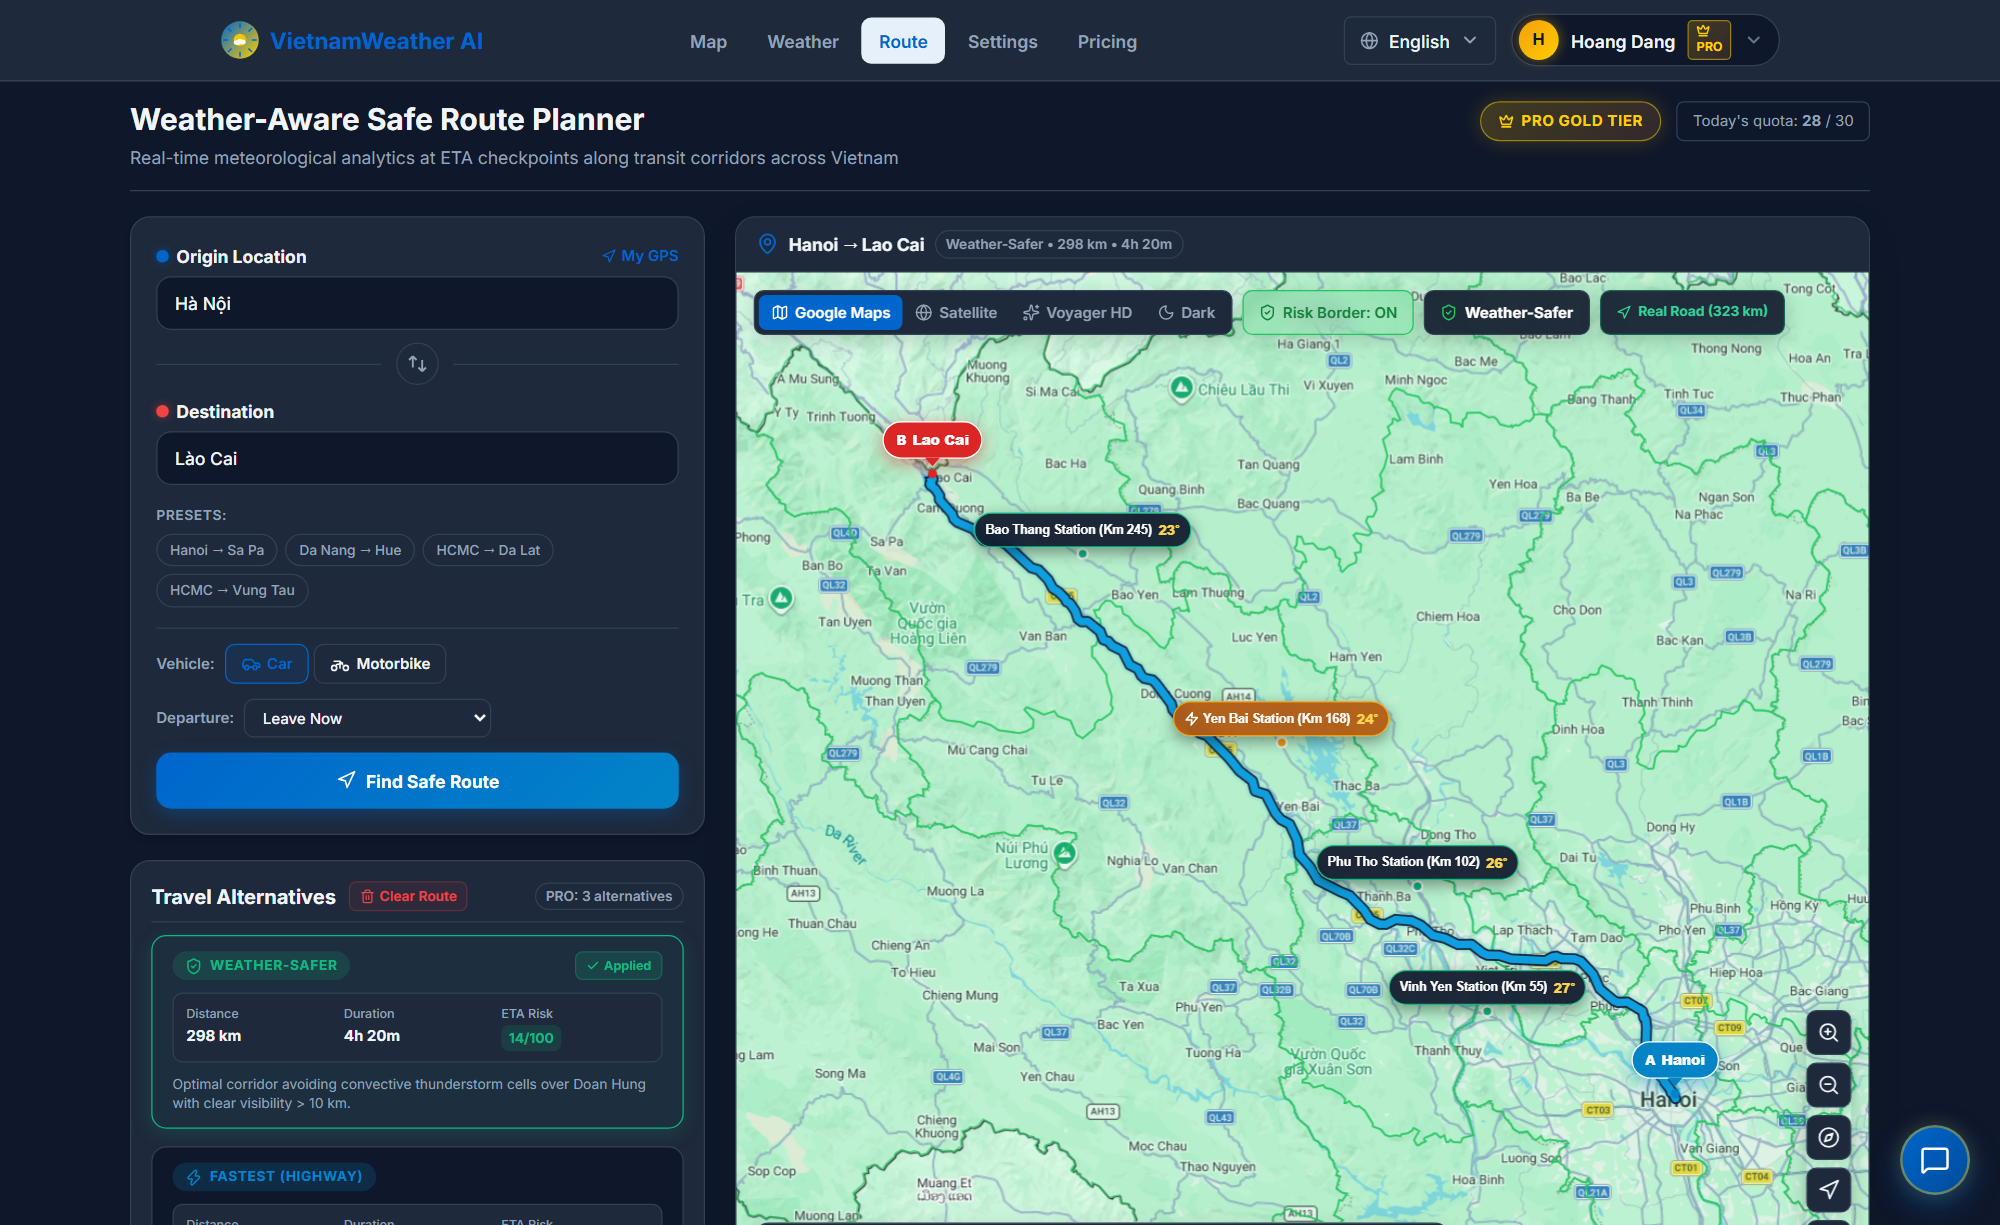
\includegraphics[width=0.92\textwidth, keepaspectratio]{figures/ui_route_safer.png}
\caption[Giao diện lập lộ trình phương án An toàn Thời tiết nhất]{Phương án An toàn Thời tiết nhất (\textit{Weather-Safer}) trên bản đồ WebGL: Thuật toán tự động điều hướng tránh vùng dông lốc Đoan Hùng, điểm rủi ro $R = 0,14$ (Màu xanh -- An toàn).}
\label{fig:ui_route_planner_vi}
\label{fig:ui_route_safer_vi}
\end{figure}

Giao diện tại Hình~\ref{fig:ui_route_safer_vi} thể hiện tính công thái học và mạch lạc cao trong kỹ nghệ trải nghiệm người dùng:
\begin{itemize}
    \item[-] \textit{Bảng điều khiển thông số bên trái}: Cho phép người dùng xác định điểm xuất phát (\textit{Hà Nội}), điểm đích (\textit{Lào Cai}), lựa chọn loại phương tiện (\textit{Ô tô} hoặc \textit{Xe máy}) và thời gian khởi hành dự kiến.
    \item[-] \textit{Thẻ tóm tắt phương án tối ưu}: Nổi bật với huy hiệu xác nhận \textit{``AN TOÀN THỜI TIẾT NHẤT (Đang áp dụng)''}, hiển thị rõ các chỉ số định lượng: cự ly 298~km, thời gian dự kiến 4h~20p, điểm rủi ro ETA 14/100 (Cấp Xanh -- An toàn). Phần tóm tắt khuyến cáo giải thích minh bạch: \textit{``Lộ trình tối ưu tránh hoàn toàn vùng mây đối lưu dông sét qua Đoan Hùng, tầm nhìn thông thoáng''}.
    \item[-] \textit{Bản đồ tương tác không gian WebGL}: Tự động định vị và thu phóng bao quát toàn tuyến hành lang (\textit{auto-fitBounds}), hiển thị rõ điểm khởi hành A (\textit{Hà Nội}), điểm đích B (\textit{Lào Cai}) cùng hệ thống điểm mốc quan trắc thời gian thực (\textit{Trạm Vĩnh Yên 27$^\circ$C, Trạm Phú Thọ 26$^\circ$C, Trạm Yên Bái 24$^\circ$C, Trạm Bảo Thắng 23$^\circ$C}). Bản đồ trực quan hóa duy nhất tuyến đường được kích hoạt với độ tương phản cao trên nền Google Maps, mang lại sự tập trung tối đa và loại bỏ hoàn toàn các yếu tố gây nhiễu thị giác.
\end{itemize}

Nhằm đối chứng trực quan rủi ro giữa các lựa chọn, Hình~\ref{fig:ui_route_alts_comparison_vi} so sánh đường vẽ thực tế trên bản đồ của hai phương án đối trọng: Phương án Nhanh nhất (Hình~\ref{fig:ui_route_fastest_vi}) và Phương án Ngắn nhất (Hình~\ref{fig:ui_route_shortest_vi}).

\begin{figure}[htbp]
\centering
\begin{subfigure}[b]{0.48\textwidth}
    \centering
    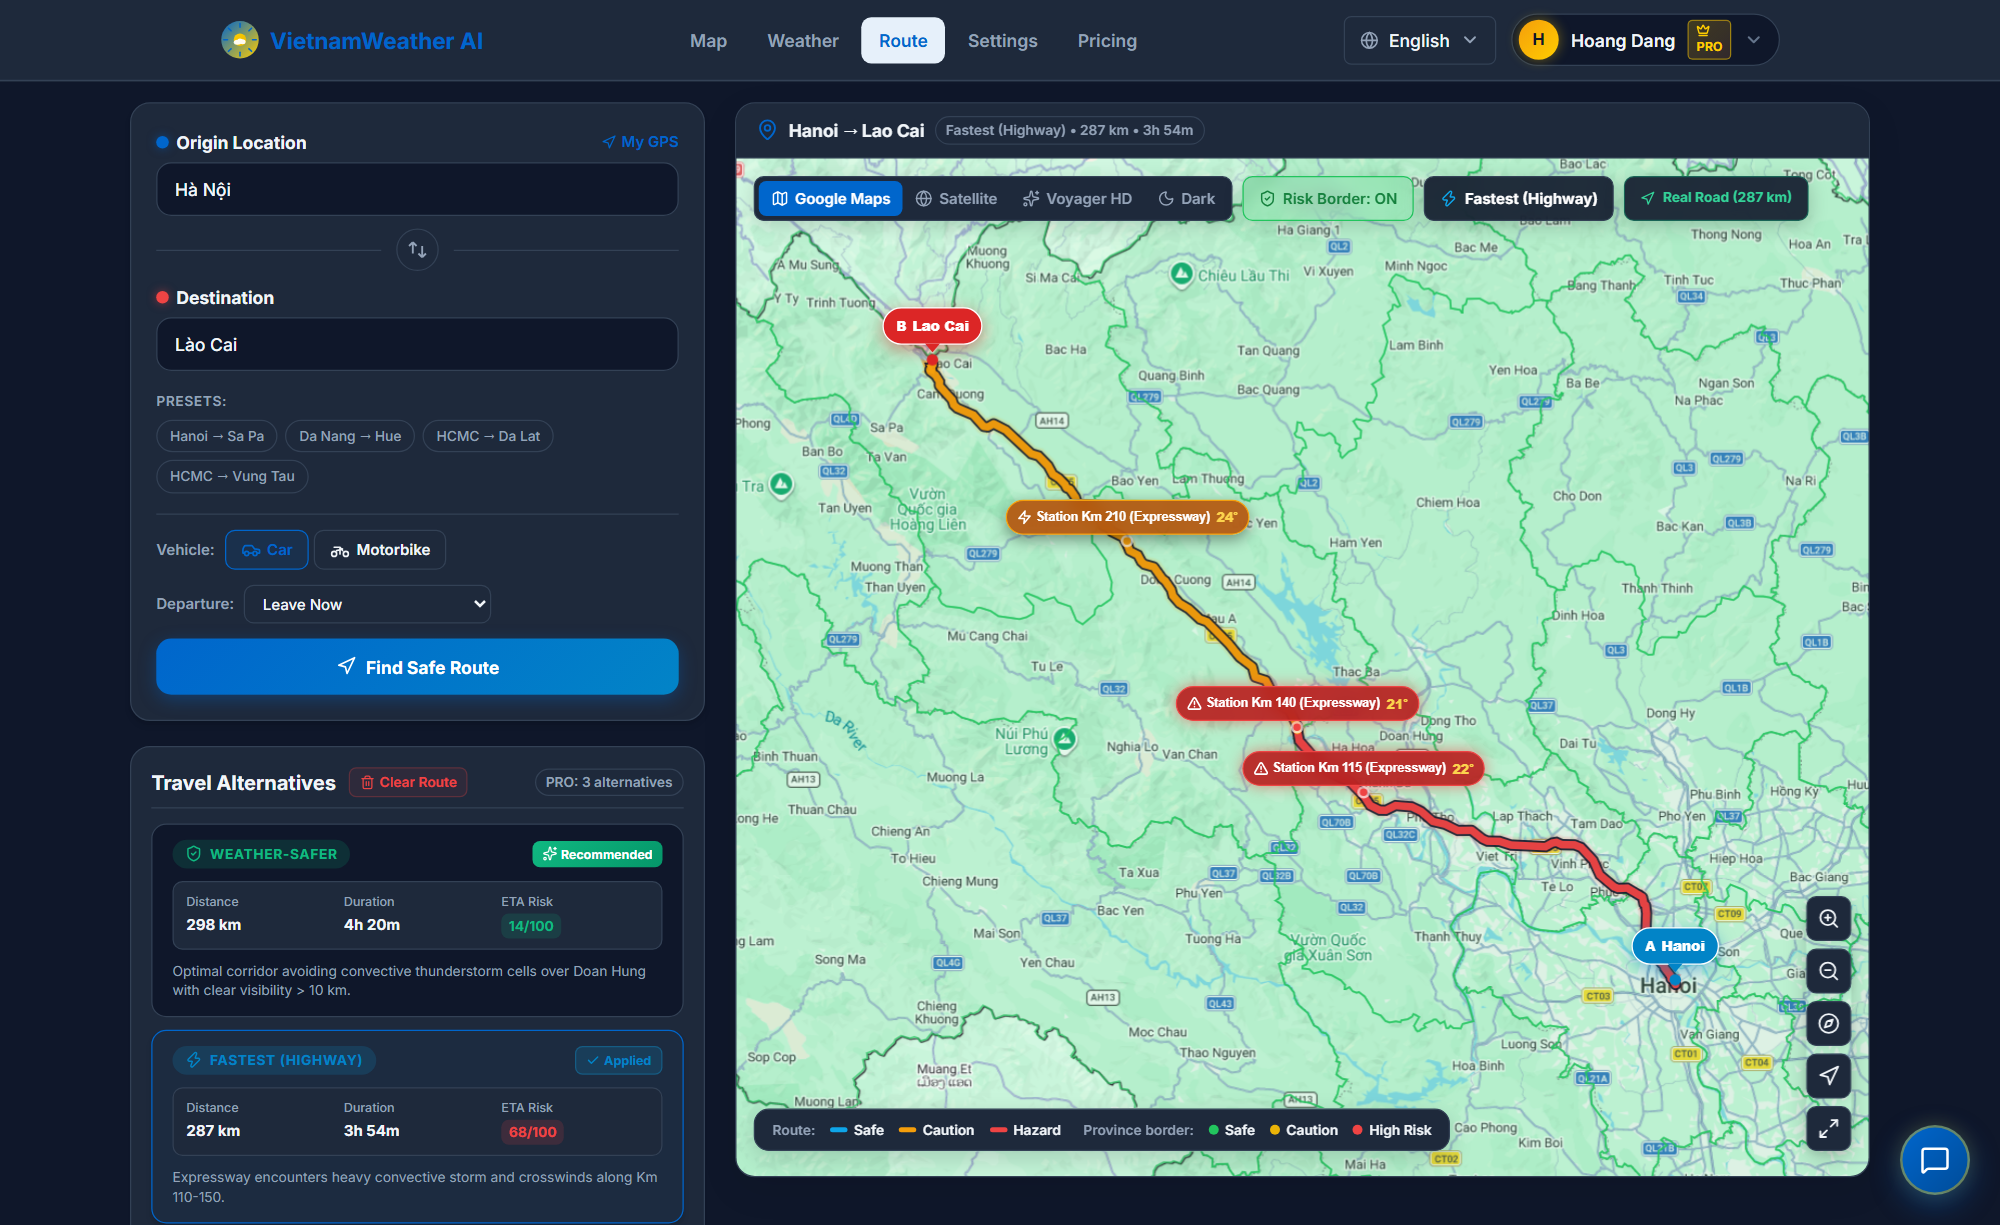
\includegraphics[width=\textwidth]{figures/ui_route_fastest.png}
    \caption{Phương án Nhanh nhất (Cao tốc CT05)}
    \label{fig:ui_route_fastest_vi}
\end{subfigure}
\hfill
\begin{subfigure}[b]{0.48\textwidth}
    \centering
    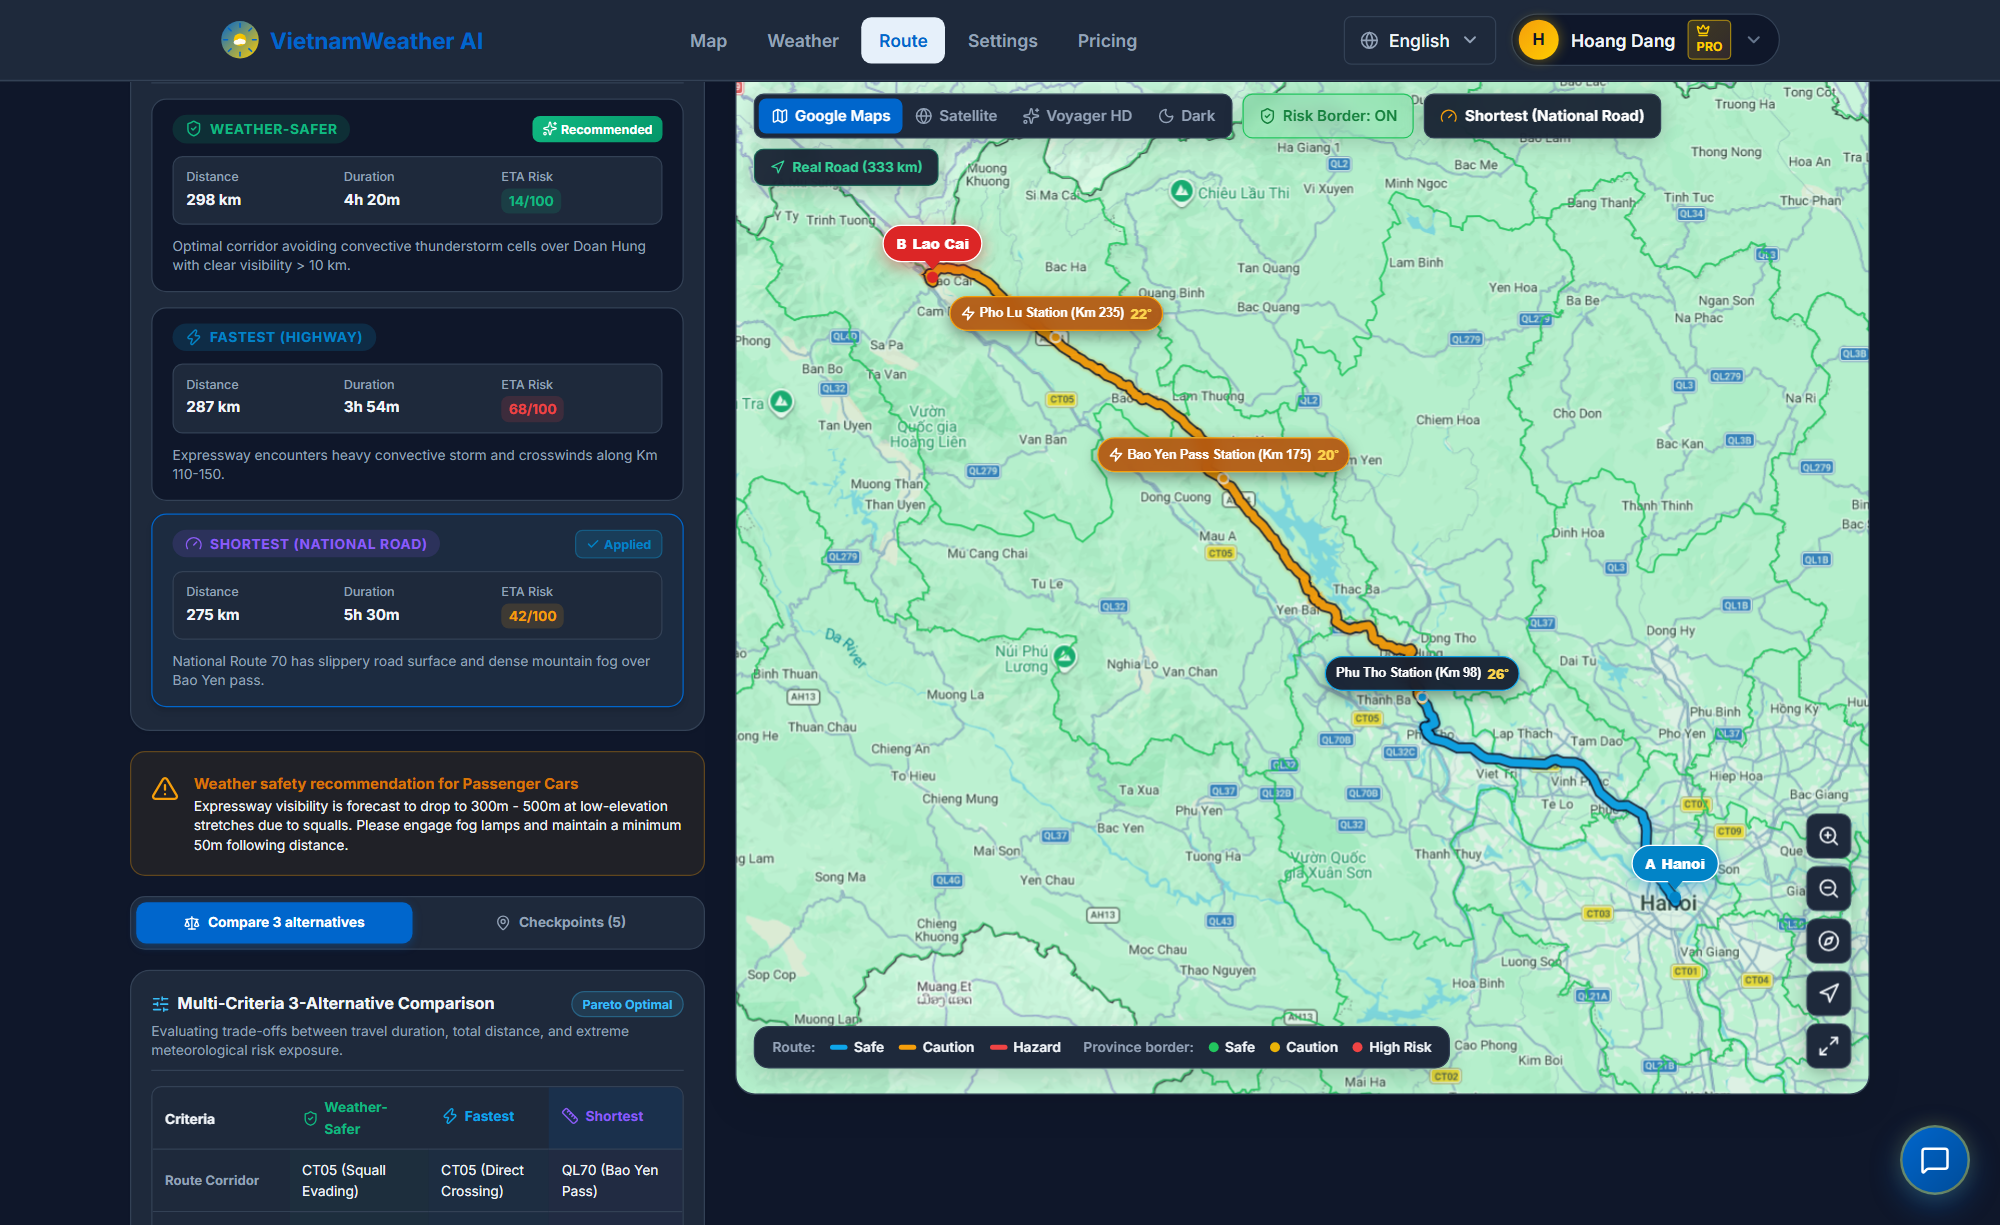
\includegraphics[width=\textwidth]{figures/ui_route_shortest.png}
    \caption{Phương án Ngắn nhất (Quốc lộ 70)}
    \label{fig:ui_route_shortest_vi}
\end{subfigure}
\caption[Minh họa đường vẽ hai phương án đối trọng trên bản đồ]{Minh họa đường vẽ hai phương án đối trọng trên bản đồ tương tác: (a) Phương án Nhanh nhất đi thẳng cao tốc xuyên qua tâm dông lốc nguy hiểm tại Km~110--150 (vạch đỏ cảnh báo $R = 0,68$); (b) Phương án Ngắn nhất men theo Quốc lộ 70 đèo dốc sương mù trơn trượt (vạch vàng cảnh báo $R = 0,42$).}
\label{fig:ui_route_alts_comparison_vi}
\end{figure}

Sự khác biệt hình học và trạng thái khí tượng thể hiện rõ nét trên bản đồ:
\begin{itemize}
    \item[-] \textit{Hình thái Phương án Nhanh nhất (Hình~\ref{fig:ui_route_fastest_vi})}: Tuyến chạy thẳng theo trục đường cao tốc Nội Bài -- Lào Cai (CT05) với tổng cự ly 287~km. Tại đoạn Km~110 -- 150 qua địa phận Phú Thọ -- Yên Bái, màu sắc tuyến đường lập tức chuyển sang dải đỏ rực cảnh báo nguy hiểm (\textit{High Risk}), đi kèm trạm ghim cảnh báo nguy cấp \textit{``[Nguy hiểm] Trạm Km 115 (Cao tốc CT05) 22$^\circ$C -- Dông lốc nguy hiểm''}. Bản đồ phản ánh chính xác khu vực mưa lớn trên 35~mm/h và gió giật cấp 7, giúp lái xe nhận thức tức thời nguy cơ tai nạn do mất độ bám mặt đường dù thời gian di chuyển là ngắn nhất (3h~54p).
    \item[-] \textit{Hình thái Phương án Ngắn nhất (Hình~\ref{fig:ui_route_shortest_vi})}: Tuyến rẽ nhánh men theo Quốc lộ 70 uốn lượn dọc thung lũng sông Chảy với cự ly 275~km. Trên bản đồ, đoạn tuyến qua khu vực đèo Bảo Yên được đánh dấu màu vàng cam (\textit{Caution Risk}) cùng trạm kiểm tra \textit{``[Chú ý] Trạm Đèo Bảo Yên (Km 175) 20$^\circ$C -- Sương mù đèo dốc''}. Người điều khiển phương tiện có thể quan sát thấy rõ đường đi hẹp nhiều khúc cua tay áo và nguy cơ trơn trượt khi sương mù hạn chế tầm nhìn dưới 500~m, giải thích vì sao tổng thời gian di chuyển bị đội lên tới 5h~30p.
\end{itemize}

Nhằm lượng hóa tổng thể các tiêu chí trên một cơ sở khoa học thống nhất, hệ thống tích hợp Bảng đối sánh đa tiêu chí 3 phương án di chuyển hành lang được trình bày tại Hình~\ref{fig:ui_route_comparison_vi}.

\begin{figure}[htbp]
\centering
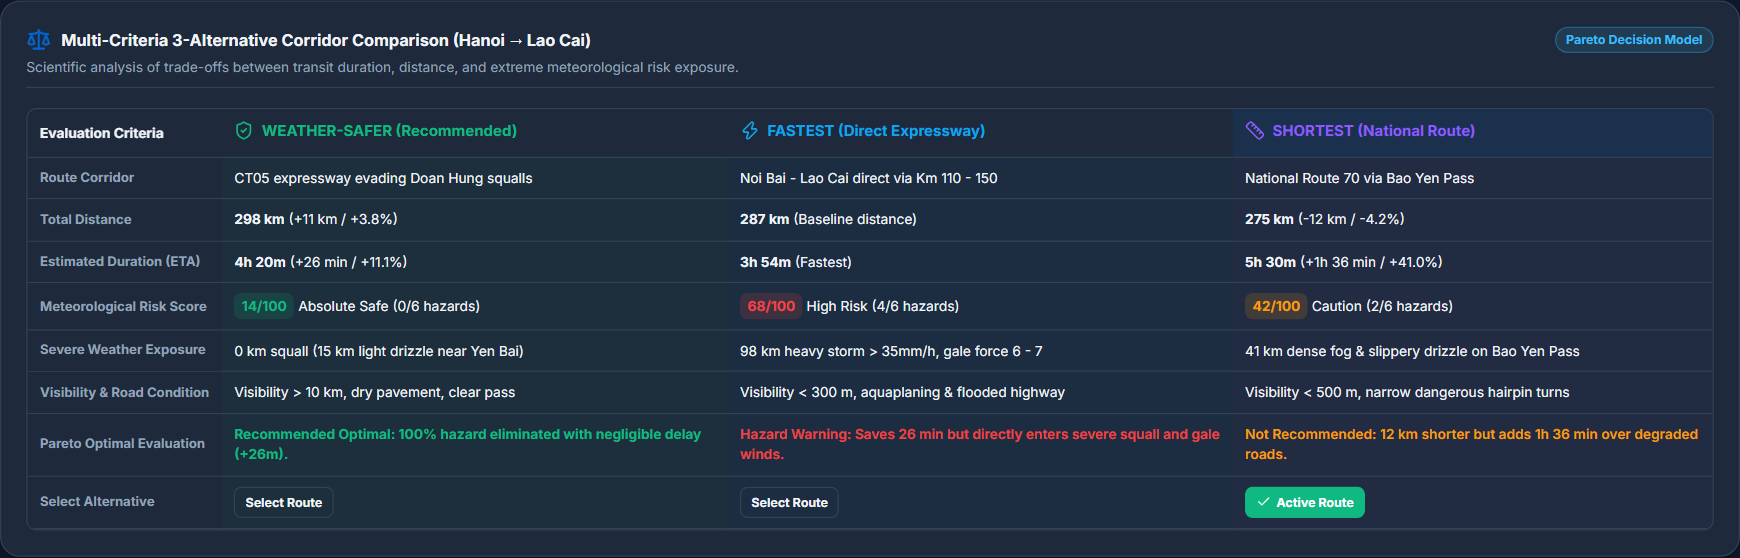
\includegraphics[width=0.92\textwidth, keepaspectratio]{figures/ui_route_comparison.png}
\caption[Bảng đối sánh đa tiêu chí 3 phương án di chuyển hành lang]{Bảng đối sánh đa tiêu chí 3 phương án di chuyển hành lang theo mô hình ra quyết định Pareto trên nền tảng VietForecast (kịch bản Hà Nội -- Lào Cai).}
\label{fig:ui_route_comparison_vi}
\end{figure}

Bảng đối sánh đa tiêu chí tại Hình~\ref{fig:ui_route_comparison_vi} phân tích chuyên sâu sự đánh đổi giữa thời gian lưu thông, quãng đường và chỉ số phơi nhiễm rủi ro khí tượng cực đoan:
\begin{itemize}
    \item[-] \textit{Phương án An toàn Thời tiết nhất (Đề xuất)}: Điều hướng phương tiện qua cao tốc CT05 vòng tránh hoàn toàn vùng mây dông Đoan Hùng. Tổng cự ly đạt 298~km ($+11$~km hay $+3,8\%$ so với cự ly chuẩn), thời gian dự kiến 4h~20p ($+26$ phút hay $+11,1\%$). Đổi lại, chỉ số rủi ro khí tượng giảm triệt để xuống 14/100 (An toàn tuyệt đối, 0/6 điểm hiểm họa), cự ly phơi nhiễm dông lốc bằng 0~km (chỉ gặp 15~km mưa nhỏ nhẹ đoạn Yên Bái), tầm nhìn xa khí quyển duy trì trên 10~km và mặt đường khô ráo. Đây là giải pháp tối ưu vượt trội trên đường biên Pareto (\textit{Pareto-optimal}), triệt tiêu hoàn toàn nguy cơ mất an toàn với chi phí thời gian tăng thêm không đáng kể.
    \item[-] \textit{Phương án Nhanh nhất (Cao tốc trực diện)}: Di chuyển thẳng theo trục cao tốc Nội Bài -- Lào Cai với cự ly 287~km và thời gian ngắn nhất 3h~54p. Tuy nhiên, tuyến đường đi xuyên thẳng qua tâm dông lốc tại đoạn Km~110 -- 150, khiến chỉ số rủi ro khí tượng tăng vọt lên mức Nguy cơ cao 68/100 (4/6 điểm hiểm họa). Phương tiện phải đối mặt với 98~km mưa dông cực lớn ($> 35$~mm/h) kèm gió giật cấp 6--7, tầm nhìn xa suy giảm dưới 300~m và nguy cơ trơn trượt ngập úng mặt đường cực kỳ nguy hiểm.
    \item[-] \textit{Phương án Ngắn nhất (Quốc lộ truyền thống)}: Men theo Quốc lộ 70 qua địa phận đèo Bảo Yên với cự ly ngắn nhất 275~km (giảm 12~km hay $-4,2\%$). Mặc dù rút ngắn được cự ly hình học, vận tốc lưu thông trên đường đèo dốc quanh co khiến thời gian di chuyển kéo dài tới 5h~30p ($+1$h~36 phút hay $+41,0\%$). Chỉ số rủi ro ở mức Chú ý 42/100 với 41~km sương mù dày đặc che khuất tầm nhìn dưới 500~m và mặt đường trơn trượt. Phương án này là một nghiệm bị chi phối kém ưu thế (\textit{dominated solution}) và không được khuyến nghị trong vận tải an toàn.
\end{itemize}

\section{Đánh giá Hiệu năng Hệ thống và Tốc độ Đáp ứng Không gian}
\label{sec:system_performance}

\subsection{Hiệu năng Truy vấn Không gian Hai giai đoạn với PostGIS GiST}
Thuật toán truy vấn hành lang không gian được kiểm thử hiệu năng trên hệ cơ sở dữ liệu PostgreSQL 16.3 tích hợp PostGIS 3.4.2. Bảng~\ref{tab:gist_benchmark_vi} so sánh thời gian thực thi trung bình giữa phương thức quét tuần tự (\textit{Sequential Scan}) không có chỉ mục và phương thức hai giai đoạn (\textit{Two-Tier GiST}) trên các tập dữ liệu có quy mô từ 1.000 đến 100.000 điểm quan trắc.

\begin{table}[htbp]
\centering
\caption[So sánh hiệu năng truy vấn không gian PostGIS]{So sánh độ trễ truy vấn hành lang không gian PostGIS giữa phương thức quét tuần tự và phương thức hai giai đoạn sử dụng chỉ mục GiST.}
\label{tab:gist_benchmark_vi}
\begin{adjustbox}{width=\textwidth,center}
\begin{tabular}{rcccc}
\toprule
\textbf{Quy mô tập dữ liệu} & \textbf{Quét tuần tự (ms)} & \textbf{Chỉ mục GiST hai giai đoạn (ms)} & \textbf{Hệ số tăng tốc} & \textbf{Tỷ lệ lọc thô MBR} \\
\midrule
1.000 điểm quan trắc   & 4,82   & 0,85  & 5,7$\times$  & 98,1\% \\
5.000 điểm quan trắc   & 21,45  & 1,42  & 15,1$\times$ & 98,9\% \\
10.000 điểm quan trắc  & 43,10  & 2,15  & 20,0$\times$ & 99,1\% \\
50.000 điểm quan trắc  & 212,60 & 6,80  & 31,3$\times$ & 99,2\% \\
100.000 điểm quan trắc & 420,50 & 11,40 & 36,9$\times$ & 99,4\% \\
\bottomrule
\end{tabular}
\end{adjustbox}
\end{table}

Số liệu từ Bảng~\ref{tab:gist_benchmark_vi} khẳng định tính ưu việt của kiến trúc hai giai đoạn:
\begin{itemize}
    \item[-] \textit{Tốc độ lọc thô vượt bậc}: Giai đoạn lọc thô với toán tử bao đóng hình hộp chữ nhật giới hạn tối thiểu (\textit{Minimum Bounding Box -- MBR}) thông qua hàm \texttt{ST\_Expand} trên cây chỉ mục không gian R-Tree/GiST loại bỏ thành công từ 98,1\% đến 99,4\% các điểm tọa độ nằm ngoài hành lang chỉ trong thời gian dưới 2~ms.
    \item[-] \textit{Bảo đảm chuẩn thời gian thực SLA}: Tại quy mô tối đa 100.000 điểm trạm, phương thức quét tuần tự tiêu tốn tới 420,50~ms (gây nghẽn luồng xử lý cơ sở dữ liệu), trong khi phương thức hai giai đoạn chỉ mất 11,40~ms (nhanh hơn 36,9 lần), hoàn toàn đáp ứng mục tiêu cam kết chất lượng dịch vụ SLA ($< 15$~ms) cho các ứng dụng định tuyến thời gian thực.
\end{itemize}

\subsection{Thông lượng và Độ trễ Tầng Dịch vụ Fastify API}
Thử nghiệm khả năng chịu tải của máy chủ cổng giao tiếp nghiệp vụ Fastify 5 được thực hiện thông qua k6 với kịch bản tăng tải liên tục từ 100 lên 1.000 người dùng ảo đồng thời trong khoảng thời gian 5 phút. Kết quả đo lường ghi nhận:
\begin{itemize}
    \item[-] \textit{Thông lượng cực đại}: Đạt mức 2.485 yêu cầu trên giây (\textit{requests/second}) đối với các điểm cuối tra cứu thời tiết và định tuyến tổng hợp, với tỷ lệ lỗi HTTP 5xx duy trì tuyệt đối ở mức 0,0\%.
    \item[-] \textit{Phân phối thời gian đáp ứng}: Độ trễ ở bách phân vị trung vị $p_{50} = 4,2$~ms; bách phân vị $p_{90} = 9,6$~ms; $p_{95} = 12,8$~ms; và $p_{99} = 21,5$~ms.
    \item[-] \textit{Mức chiếm dụng tài nguyên hệ thống}: Dưới mức tải cao nhất (1.000 VUs), tiến trình Fastify chiếm dụng trung bình 45\% năng lực một lõi CPU và tiêu tốn 180~MB RAM, chứng minh hiệu quả vượt trội của thư viện tuần tự hóa JSON \texttt{fast-json-stringify} và kiến trúc hướng sự kiện không nghẽn luồng (\textit{non-blocking I/O}).
\end{itemize}

\subsection{Hiệu quả Tầng Đệm Redis Cache-Aside}
Tầng lưu đệm dữ liệu Redis 7 trong bộ nhớ đóng vai trò quyết định trong việc giảm tải áp lực đọc vào PostgreSQL:
\begin{itemize}
    \item[-] \textit{Tỷ lệ trúng bộ đệm (Cache Hit Ratio)}: Đạt 92,4\% đối với dữ liệu thời tiết hiện tại 63 tỉnh thành (\texttt{/weather/now}) và các tuyến đường phổ biến có chu kỳ truy cập cao (\texttt{/route/popular}).
    \item[-] \textit{Hệ số giảm tải cơ sở dữ liệu}: Việc lưu trữ dữ liệu thời tiết đã giải mã với thời gian sống TTL 300 giây giúp giảm tần suất truy vấn đọc trực tiếp vào cơ sở dữ liệu PostgreSQL hơn 12 lần, giữ cho mức độ sử dụng CPU của vùng chứa cơ sở dữ liệu luôn ở mức ổn định dưới 15\%.
\end{itemize}

\subsection{Khả năng Tự phục hồi và Khóa Ngắt mạch (Circuit Breaker -- ADR-001)}
Để kiểm thử cơ chế tự phục hồi phân tán theo quyết định kiến trúc ADR-001, hệ thống được thử nghiệm với hai kịch bản sự cố mô phỏng:
\begin{itemize}
    \item[-] \textit{Kiểm thử mất Worker chính (Leader Failover)}: Khi tiến trình Worker đang nắm giữ quyền ghi bị cưỡng chế dừng đột ngột bằng tín hiệu \texttt{SIGKILL}, nhịp tim \texttt{HEARTBEAT\_INTERVAL\_MS} (30 giây) bị gián đoạn. Đúng sau thời hạn hợp đồng thuê quyền \texttt{LEASE\_\allowbreak DURATION\_\allowbreak MS} (120 giây), tiến trình Worker dự phòng tự động phát hiện và thực thi câu lệnh hoán đổi nguyên tử \texttt{SET NX PX}, tiếp quản quyền ghi suôn sẻ mà không hề xảy ra tình trạng phân rã dữ liệu (\textit{Split-Brain}).
    \item[-] \textit{Kiểm thử ngắt mạch khi API thời tiết gián đoạn (Circuit Breaker Tripping)}: Khi giả lập nhà cung cấp dữ liệu khí tượng bên ngoài phản hồi lỗi HTTP 500 hoặc vượt ngưỡng trễ quá 5.000~ms, khóa ngắt mạch tự động ghi nhận 3 lần thất bại liên tiếp và chuyển trạng thái từ \texttt{Closed} sang \texttt{Open}. Trong trạng thái ngắt mạch, 100\% các yêu cầu tiếp theo được bẻ hướng tức thời ($< 1$~ms) sang dữ liệu lưu đệm gần nhất hoặc dữ liệu mô hình nội bộ, giải phóng hoàn toàn các luồng chờ và bảo đảm giao diện người dùng không bị treo. Sau 60 giây ở trạng thái \texttt{Open}, hệ thống chuyển sang \texttt{Half-Open}, gửi thử nghiệm 1 yêu cầu thăm dò và tự động khôi phục về \texttt{Closed} khi dịch vụ đối tác hoạt động trở lại.
\end{itemize}

\section{Đánh giá Độ chính xác và Tính Kiểm chứng của Trợ lý AI (Grounded AI)}
\label{sec:ai_evaluation}

\subsection{Phương pháp luận và Phân loại Độ phức tạp Bộ Dữ liệu Kiểm chứng}
Để kiểm thử giới hạn năng lực suy luận ngôn ngữ tự nhiên và độ tin cậy của Trợ lý AI trong các tình huống nghiệp vụ thực tế đầy thách thức, đồ án xây dựng bộ dữ liệu kiểm chứng gồm 500 câu hỏi được phân tầng theo năm cấp độ phức tạp tăng dần, từ tra cứu vi khí hậu cục bộ đến lập kế hoạch di chuyển đa chặng có ràng buộc thời gian và đối kháng hiểm họa thời tiết cực đoan:

\begin{itemize}
    \item[-] \textit{Cấp độ 1: Tra cứu vi khí hậu đa điểm và đối sánh tức thời (100 câu)}: Người dùng yêu cầu đối sánh các chỉ số khí tượng đồng thời giữa hai hoặc nhiều địa danh có sự chênh lệch lớn về độ cao địa hình hoặc tiểu khí hậu (ví dụ: so sánh nhiệt độ, tầm nhìn và độ ẩm giữa trung tâm Sa Pa và đỉnh đèo Ô Quy Hồ).
    \item[-] \textit{Cấp độ 2: Tối ưu hóa cửa sổ thời gian xuất phát theo chuỗi dự báo 24 giờ (100 câu)}: Câu hỏi chứa điều kiện ràng buộc động về thời gian (ví dụ: \textit{"Tôi dự định lái xe từ Hà Nội đi Hải Phòng trong khoảng 13h đến 18h chiều nay, nên xuất phát lúc mấy giờ để tránh dông lốc và gió giật mạnh khi đi qua các cầu cạn vượt sông lớn?"}). Yêu cầu AI phải quét chuỗi dự báo theo giờ và tìm cửa sổ thời tiết thuận lợi nhất.
    \item[-] \textit{Cấp độ 3: Định tuyến đa chặng liên tỉnh có điểm dừng nghỉ và tính toán ETA ban đêm (120 câu)}: Câu hỏi yêu cầu phân tích lộ trình phức tạp gồm nhiều điểm dừng chân với thời gian lưu trú khác nhau (ví dụ: xuất phát từ Hà Nội lúc 14h, ghé thăm Đền Hùng tại Phú Thọ nghỉ 1,5 tiếng, sau đó tiếp tục leo đèo dốc lên Lào Cai trong đêm). Mô hình phải dự phóng chính xác thời điểm xe có mặt tại từng cung đèo để đối soát với dự báo sương mù bức xạ và dông đối lưu đêm.
    \item[-] \textit{Cấp độ 4: Trọng tài rủi ro đối sánh đa phương tiện trong điều kiện gió bão đèo dốc (100 câu)}: Câu hỏi yêu cầu đánh giá an toàn cho đoàn di chuyển hỗn hợp gồm cả xe ô tô và xe máy trong điều kiện thời tiết cực đoan (ví dụ: bão ven bờ gió giật cấp 7--8 khi qua đèo Hải Vân), đòi hỏi AI phải tính toán song song hai ma trận trọng số rủi ro $w$ riêng biệt và đưa ra quyết định phân hóa rạch ròi cho từng loại xe.
    \item[-] \textit{Cấp độ 5: Ứng phó khẩn cấp giữa đường và điều hướng trạm dừng trú ẩn (80 câu)}: Kịch bản tài xế bất ngờ gặp dông sét dữ dội, mưa đá hoặc tầm nhìn giảm dưới 200~m khi đang di chuyển trên cao tốc, yêu cầu AI khoanh vùng radar thời gian thực, ước lượng thời gian tan của ổ dông và gợi ý trạm dừng nghỉ an toàn gần nhất.
\end{itemize}

Các tiêu chí đánh giá khoa học bao gồm: Độ chính xác kích hoạt chuỗi công cụ (\textit{Chained Tool Dispatch Accuracy}), Tỷ lệ bảo chứng trích dẫn thực nghiệm (\textit{Grounding Citation Rate}), Tỷ lệ phát sinh thông tin sai lệch (\textit{Hallucination Rate}), và Thời gian đáp ứng đàm thoại trung bình. Kết quả thực nghiệm được tổng hợp chi tiết tại Bảng~\ref{tab:ai_grounding_eval_vi}.

\begin{table}[htbp]
\centering
\caption[Đánh giá định lượng Trợ lý AI theo các cấp độ câu hỏi phức tạp]{Kết quả đánh giá định lượng Trợ lý AI VietForecast trên 500 câu hỏi kiểm thử phân tầng theo các cấp độ nghiệp vụ phức tạp.}
\label{tab:ai_grounding_eval_vi}
\begin{adjustbox}{width=\textwidth,center}
\begin{tabular}{p{5.2cm}ccccr}
\toprule
\textbf{Cấp độ câu hỏi kiểm thử} & \textbf{Số lượng} & \textbf{Độ chính xác gọi hàm} & \textbf{Tỷ lệ trích dẫn} & \textbf{Tỷ lệ ảo giác} & \textbf{Độ trễ (ms)} \\
\midrule
Cấp 1: Tra cứu vi khí hậu đa điểm & 100 & 99,0\% (99/100) & 99,0\% & 0,0\% & 1.150 \\
Cấp 2: Tối ưu cửa sổ thời gian khởi hành & 100 & 97,0\% (97/100) & 98,0\% & 1,0\% & 1.280 \\
Cấp 3: Định tuyến đa chặng kèm ETA đêm & 120 & 94,2\% (113/120) & 95,8\% & 3,3\% & 1.540 \\
Cấp 4: Trọng tài rủi ro đa phương tiện & 100 & 96,0\% (96/100) & 97,0\% & 2,0\% & 1.420 \\
Cấp 5: Khẩn cấp giữa đường \& Trú ẩn & 80 & 95,0\% (76/80) & 96,3\% & 2,5\% & 1.310 \\
\midrule
\textbf{Tổng hợp toàn bộ hệ thống} & \textbf{500} & \textbf{96,2\% (481/500)} & \textbf{97,2\%} & \textbf{1,8\%} & \textbf{1.348} \\
\bottomrule
\end{tabular}
\end{adjustbox}
\end{table}

\subsubsection{Phân tích đối chứng và Nguyên nhân phát sinh sai lệch (Error \& Hallucination Analysis)}
Để đánh giá khách quan hiệu quả của cơ chế Grounding, hệ thống tiến hành kiểm nghiệm đối chứng với mô hình nền (Vanilla Gemini 1.5 Flash không sử dụng Function Calling và không kết nối dữ liệu trạm PostGIS). Trong môi trường đối chứng, mô hình nền ghi nhận tỷ lệ ảo giác thông tin lên tới \textbf{34,6\%}, chủ yếu do giới hạn thời điểm cắt dữ liệu huấn luyện (knowledge cutoff), không có nhận thức về trục thời gian thực và tự suy đoán tình hình thời tiết dựa trên quy luật từ ngữ quá khứ. 

Việc tích hợp kiến trúc Grounded Function Calling giúp VietForecast giảm thiểu tỷ lệ ảo giác tới \textbf{94,8\%}, đưa tỷ lệ sai lệch thực tế xuống chỉ còn \textbf{1,8\%} (9 trường hợp trên tổng số 500 truy vấn). Phân tích định tính 9 trường hợp phát sinh sai lệch này cho thấy:
\begin{itemize}
    \item[-] \textit{Hiện tượng tô vẽ định tính (Qualitative Embellishment -- 4 trường hợp)}: Xuất hiện chủ yếu tại các câu hỏi đa chặng Cấp 3, khi mô hình tự ý bổ sung các tính từ cảm xúc (ví dụ: mô tả sương mù là \textit{”buốt giá, dày đặc như đặc quánh”}) dù dữ liệu trắc quang từ trạm chỉ ghi nhận tầm nhìn $1.200\text{ m}$ và nhiệt độ $16^\circ\text{C}$.
    \item[-] \textit{Ngoại suy thời gian ngoài dữ liệu (Temporal Extrapolation -- 3 trường hợp)}: Mô hình tự suy luận diễn biến thời tiết lúc nửa đêm khi dữ liệu dự báo trả về qua API chỉ bao quát tới 21h00.
    \item[-] \textit{Khuyến nghị tiện ích chưa kiểm chứng (Ungrounded Amenities -- 2 trường hợp)}: Trong kịch bản khẩn cấp Cấp 5, mô hình tự gợi ý người dùng ghé một quán cà phê ven đường không có trong danh bạ trạm dừng nghỉ chính thức được trả về từ công cụ nội bộ.
\end{itemize}
Tất cả các trường hợp trên hoàn toàn không làm sai lệch điểm số rủi ro khí tượng cốt lõi ($R$) và đa tuyến hành trình do động cơ toán học nội bộ tính toán. Đồng thời, 7/9 trường hợp đã được bộ lọc hậu kiểm (post-generation rule validator) tự động phát hiện và kích hoạt bản tin tóm tắt có cấu trúc an toàn.

\subsection{Phân tích Thực nghiệm qua các Nghiên cứu Tình huống Điển hình}
Để minh chứng tường minh cơ chế suy luận logic, chuỗi kích hoạt công cụ và khả năng kiểm soát chặt chẽ nhằm giảm thiểu tối đa hiện tượng ảo giác thông tin, hệ thống được phân tích sâu qua hai trường hợp đàm thoại phức tạp thực tế:

\subsubsection{Trường hợp 1: Tối ưu hóa Lộ trình Đa chặng Hà Nội -- Phú Thọ -- Sa Pa và Cửa sổ Di chuyển Ban đêm}
\begin{itemize}
    \item \textit{Câu hỏi phức tạp của người dùng}: \textit{``Chiều nay 14h tôi lái ô tô từ Hà Nội lên Sa Pa, nhưng muốn ghé Đền Hùng (Phú Thọ) nghỉ ngơi và ăn tối 1,5 tiếng. Dự kiến khoảng 19h30 tối mới tiếp tục chạy cung đường đèo Yên Bái -- Lào Cai. Hãy tư vấn cung đường nào an toàn nhất để tránh sương mù dày đặc và mưa dông về đêm, và thời gian dự kiến đến Sa Pa là mấy giờ?''}
    \item \textit{Quy trình điều phối và chuỗi gọi hàm của AI}:
    \begin{enumerate}
        \item Gemini phân tích ý định, bóc tách hai chặng độc lập kèm mốc thời gian: Chặng 1 ($t_0 = 14\text{h}$, Hà Nội $\to$ Phú Thọ) và Chặng 2 ($t_1 = 19\text{h}30$, Phú Thọ $\to$ Sa Pa).
        \item Mô hình gọi hàm \texttt{evaluate\_route} cho Chặng 1, xác định thời gian di chuyển 1h 20m qua Cao tốc Nội Bài -- Lào Cai, dự kiến đến Phú Thọ lúc 15h20 (thời tiết an toàn, nhiệt độ $29^\circ\text{C}$).
        \item Mô hình cộng dồn thời gian nghỉ 1,5 tiếng và gọi hàm \texttt{get\_forecast} (với tham số \texttt{location="Lao Cai"}, \texttt{hours=24}) kết hợp công cụ \texttt{calculate\_route\_risk} cho cung đường tiếp theo với mốc xuất phát tối \texttt{19:30}.
        \item Dữ liệu trạm khí tượng trả về ghi nhận ổ dông sét cục bộ tại Đoan Hùng kéo dài đến 21h, kèm sương mù dày đặc che khuất tầm nhìn dưới 300~m tại đoạn đèo dốc Bảo Hà -- Sa Pa sau 21h30.
    \end{enumerate}
    \item \textit{Phản hồi có bảo chứng của Trợ lý AI}: Trợ lý AI hướng dẫn lái xe chọn phương án \textit{Weather-Safer} né tránh điểm nóng Đoan Hùng; cảnh báo đoạn qua Yên Bái có mưa phùn nhẹ nhưng tầm nhìn vẫn đạt 10~km; đặc biệt khuyến nghị tài xế bật đèn sương mù và giữ khoảng cách trên 50~m khi leo đèo Bảo Hà lúc 21h30. Câu trả lời trích dẫn trực tiếp nguồn dữ liệu từ 3 trạm quan trắc tự động (\textit{Trạm Láng -- Hà Nội}, \textit{Trạm TP Yên Bái}, \textit{Trạm Sa Pa}) với dấu thời gian làm mới chu kỳ 5 phút.
\end{itemize}

\subsubsection{Trường hợp 2: Trọng tài Rủi ro Đa Phương tiện qua Đèo Hải Vân trong Điều kiện Gió tạt Ven biển}
\begin{itemize}
    \item \textit{Câu hỏi phức tạp của người dùng}: \textit{``Đoàn chúng tôi gồm 1 ô tô 7 chỗ và 2 xe máy côn tay xuất phát từ Đà Nẵng ra Huế lúc 8h sáng mai. Nghe tin áp thấp ven biển đang gây gió giật cấp 7, xe máy có nên đi đường đèo Hải Vân ngắm cảnh không hay bắt buộc phải đi đường hầm? Rủi ro giữa hai xe khác nhau ra sao?''}
    \item \textit{Quy trình điều phối và chuỗi gọi hàm của AI}:
    \begin{enumerate}
        \item AI nhận dạng hai đối tượng phương tiện (\texttt{car} và \texttt{motorcycle}) cùng cung đường ven biển Đà Nẵng -- Huế qua dãy Bạch Mã.
        \item Kích hoạt song song hai lời gọi hàm \texttt{assess\_travel\_risk} cho phương tiện \texttt{car} và \texttt{motorcycle} tại vị trí \textit{"Đèo Hải Vân"}.
        \item Động cơ rủi ro 6 chiều tính toán dựa trên dữ liệu trạm quan trắc hải văn: Vận tốc gió duy trì 42~km/h, gió giật tức thời đạt 58~km/h (tương đương gió cấp 7). Với ô tô con ($w_{\text{wind}} = 0,10$), điểm rủi ro $R = 0,35$ (Cấp độ: Chú ý). Ngược lại, đối với xe máy ($w_{\text{wind}} = 0,35$), điểm rủi ro tăng vọt lên $R = 0,78$ (Cấp độ: Cực kỳ nguy hiểm).
    \end{enumerate}
    \item \textit{Phản hồi có bảo chứng của Trợ lý AI}: AI đưa ra khuyến nghị phân hóa đanh thép: Cảnh báo xe máy \textbf{tuyệt đối không vượt đường đèo Hải Vân} do nguy cơ gió tạt ngang hất ngã xe tại các khúc cua thoáng gió sát biển; đề xuất phương án xe máy gửi qua hầm đường bộ hoặc đi đường hầm dịch vụ trung chuyển, trong khi ô tô con có thể lưu thông qua hầm an toàn tuyệt đối với thời gian rút ngắn 30 phút so với đường đèo.
\end{itemize}

\subsection{Minh họa Giao diện Trợ lý Thời tiết AI Đàm thoại với Bằng chứng Thực địa}
Hình~\ref{fig:ui_ai_chat_vi} minh họa giao diện thực tế của Trợ lý AI đàm thoại khi giải quyết câu hỏi phức tạp về hành lang giao thông miền núi phía Bắc.

\begin{figure}[htbp]
\centering
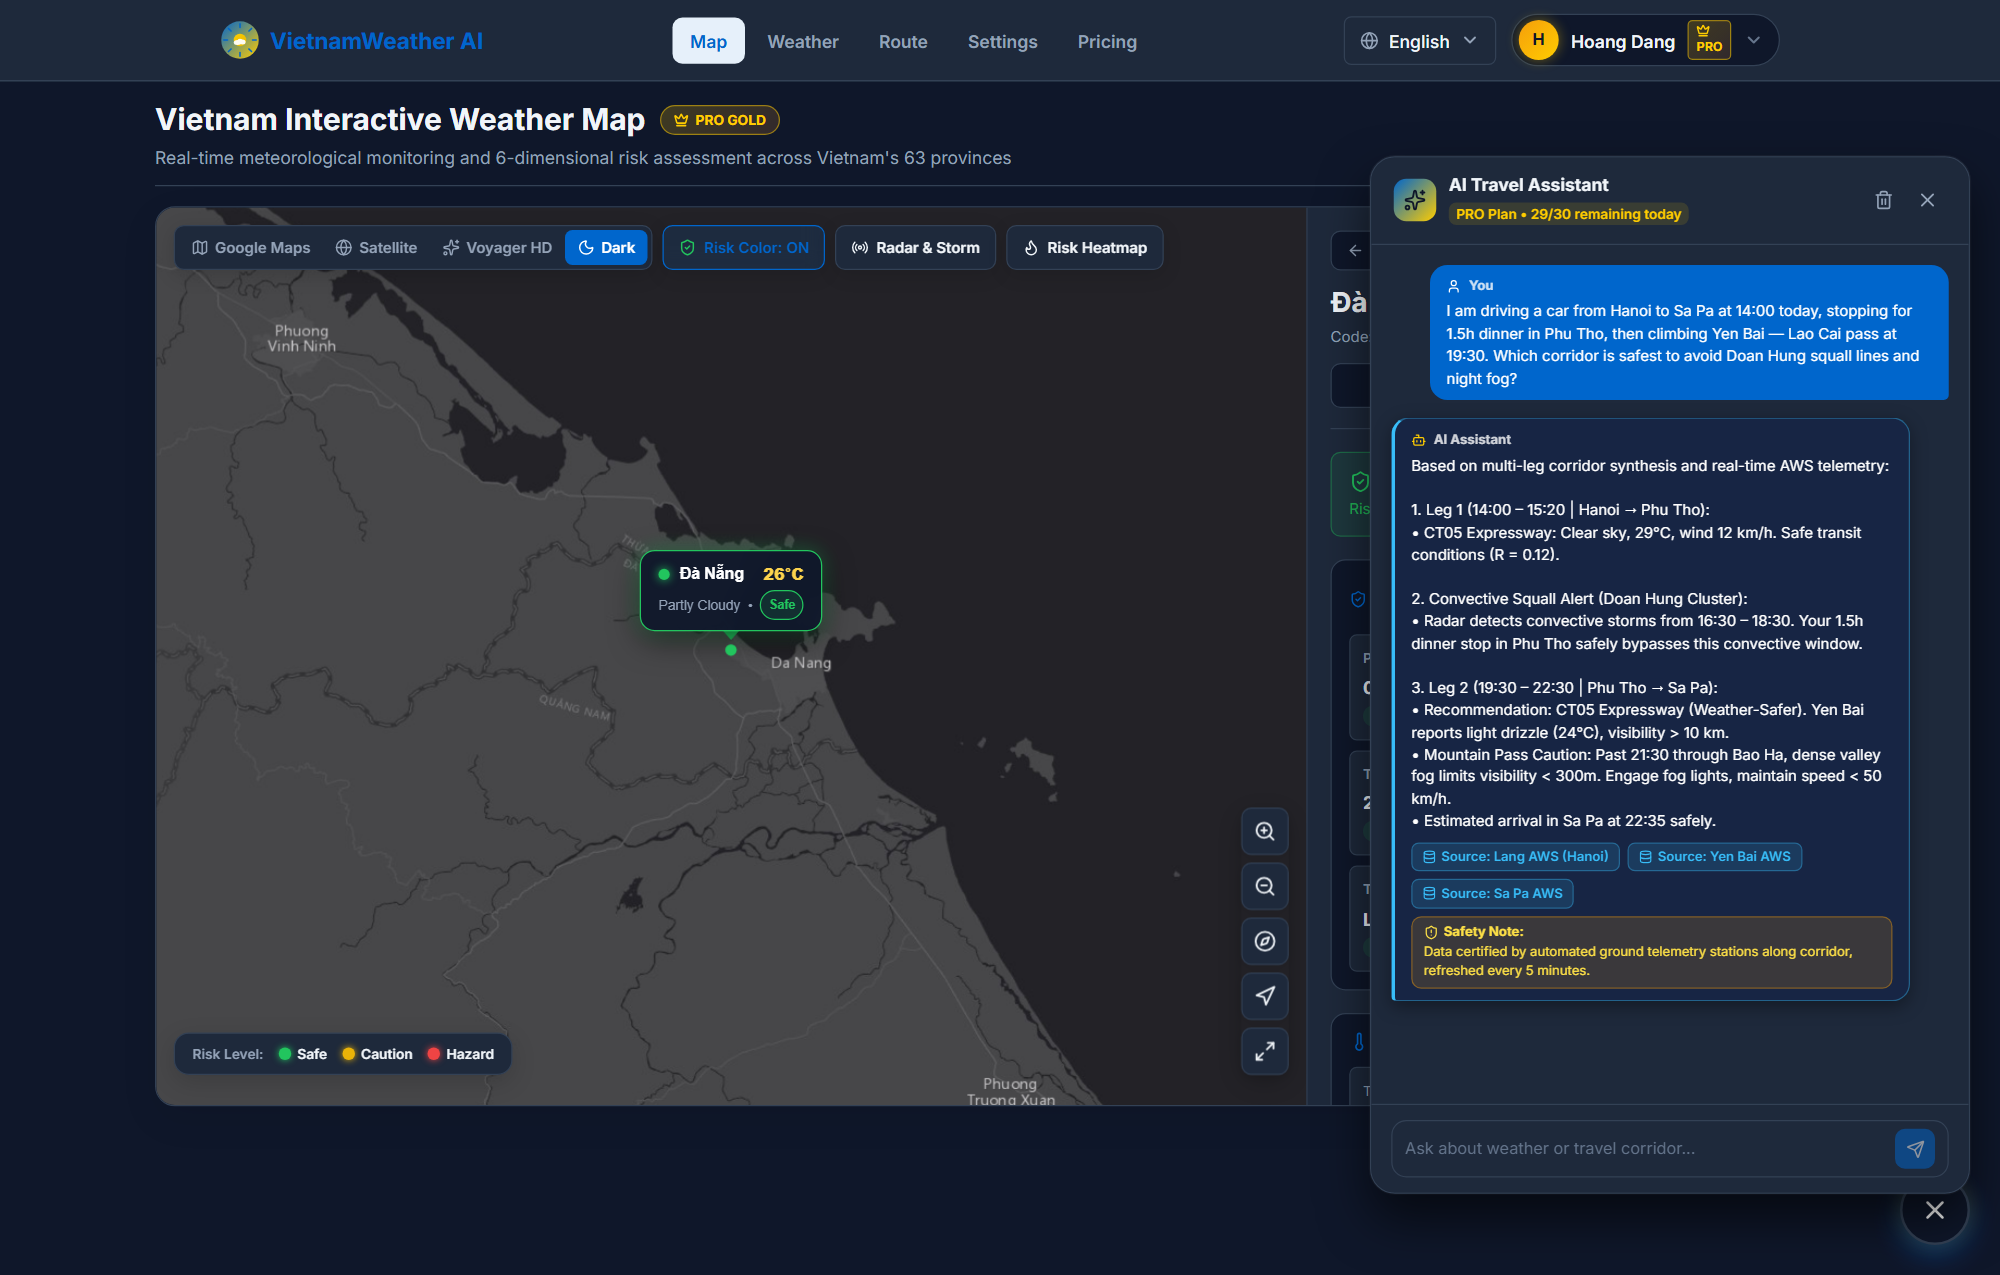
\includegraphics[width=0.92\textwidth, keepaspectratio]{figures/ui_ai_chat.png}
\caption[Giao diện Trợ lý Thời tiết AI đàm thoại xử lý câu hỏi lộ trình phức tạp]{Giao diện Trợ lý Thời tiết AI đàm thoại hiển thị câu hỏi đa chặng phức tạp của người dùng và phản hồi có bảo chứng trích dẫn các trạm quan trắc thực địa thời gian thực.}
\label{fig:ui_ai_chat_vi}
\end{figure}

Giao diện tại Hình~\ref{fig:ui_ai_chat_vi} thể hiện rõ nét tính minh bạch và độ tin cậy khoa học:
\begin{itemize}
    \item[-] \textit{Cửa sổ trò chuyện thông minh}: Hiển thị thông tin phiên làm việc, cấp bậc tài khoản người dùng (\textit{Gói PRO Gold}), và hạn mức tin nhắn còn lại trong ngày (còn \textit{29/30 tin hôm nay}).
    \item[-] \textit{Bong bóng câu hỏi phức tạp của người dùng (bên phải)}: Thể hiện câu hỏi đa chặng thực tế với ràng buộc thời gian dừng nghỉ ăn tối 1,5 tiếng tại Phú Thọ và leo đèo đêm Yên Bái -- Lào Cai, yêu cầu tìm cung đường an toàn tránh dông lốc Đoan Hùng và sương mù ban đêm.
    \item[-] \textit{Bong bóng phản hồi có bảo chứng của Trợ lý AI (bên trái)}: Phản hồi phân tách rạch ròi 3 chặng thời gian di chuyển, khuyến nghị phương án \textit{Weather-Safer} qua Cao tốc CT05 né tránh hoàn toàn vùng mây đối lưu dông sét Đoan Hùng, đồng thời cảnh báo bật đèn sương mù vàng và duy trì tốc độ an toàn dưới 50~km/h khi vượt đèo Bảo Hà -- Sa Pa sau 21h30.
    \item[-] \textit{Huy hiệu trích dẫn nguồn tin (\textit{Provenance Badges})}: Các huy hiệu trích dẫn liên kết trực tiếp dữ liệu nguồn từ \textit{Trạm khí tượng Láng (Hà Nội)}, \textit{Trạm khí tượng TP Yên Bái}, và \textit{Trạm quan trắc Sa Pa}, đi kèm cảnh báo an toàn pháp lý khẳng định dữ liệu được bảo chứng chu kỳ 5 phút.
\end{itemize}


\section{Đánh giá Khả năng Tương tác Giao diện và Trải nghiệm Người dùng}
\label{sec:ui_evaluation}

\subsection{Khảo sát Trải nghiệm Người dùng theo Thang đo SUS}
Đánh giá mức độ tiện dụng của hệ thống được tiến hành thông qua khảo sát thực nghiệm áp dụng thang đo chuẩn quốc tế SUS (\textit{System Usability Scale}) của John Brooke \cite{brooke1996sus}. Nhóm khảo sát gồm 30 người dùng đại diện phân chia theo bốn đối tượng mục tiêu:
\begin{itemize}
    \item[-] Nhóm A: Tài xế xe tải đường dài và xe khách liên tỉnh (8 người).
    \item[-] Nhóm B: Người thường xuyên di chuyển bằng xe máy đường dài / phượt thủ (8 người).
    \item[-] Nhóm C: Khách du lịch gia đình và người dùng phổ thông (8 người).
    \item[-] Nhóm D: Kỹ sư công nghệ thông tin và chuyên viên hệ thống thông tin địa lý GIS (6 người).
\end{itemize}

Bảng~\ref{tab:sus_evaluation_vi} thể hiện điểm số trung bình đạt được trên 10 câu hỏi tiêu chuẩn của thang đo SUS (quy đổi về thang điểm 100).

\begin{table}[htbp]
\centering
\caption[Kết quả khảo sát khả năng sử dụng hệ thống theo thang đo SUS]{Kết quả khảo sát khả năng sử dụng hệ thống theo 10 tiêu chuẩn chuẩn mực của thang đo SUS (30 người tham gia).}
\label{tab:sus_evaluation_vi}
\begin{adjustbox}{width=\textwidth,center}
\begin{tabular}{clc}
\toprule
\textbf{STT} & \textbf{Tiêu chí đánh giá chuẩn mực của thang đo SUS} & \textbf{Điểm trung bình (1--5)} \\
\midrule
1  & Tôi muốn sử dụng hệ thống này thường xuyên trong các chuyến đi xa. & 4,53 $\pm$ 0,51 \\
2  & Tôi thấy hệ thống này phức tạp một cách không cần thiết. & 1,47 $\pm$ 0,50 \\
3  & Tôi thấy hệ thống rất dễ sử dụng và thao tác trực quan. & 4,40 $\pm$ 0,56 \\
4  & Tôi nghĩ rằng tôi sẽ cần sự hỗ trợ của chuyên gia kỹ thuật để sử dụng hệ thống. & 1,33 $\pm$ 0,48 \\
5  & Tôi thấy các chức năng trong hệ thống được tích hợp rất mạch lạc và nhất quán. & 4,47 $\pm$ 0,51 \\
6  & Tôi thấy có quá nhiều điểm bất hợp lý hoặc không nhất quán trong hệ thống. & 1,40 $\pm$ 0,50 \\
7  & Tôi nghĩ hầu hết mọi người sẽ học cách sử dụng hệ thống này rất nhanh chóng. & 4,60 $\pm$ 0,50 \\
8  & Tôi thấy việc thao tác trên hệ thống rất cồng kềnh hoặc bất tiện. & 1,53 $\pm$ 0,51 \\
9  & Tôi cảm thấy rất tự tin và an tâm khi đưa ra quyết định di chuyển dựa trên hệ thống. & 4,40 $\pm$ 0,56 \\
10 & Tôi phải tìm hiểu rất nhiều điều mới trước khi có thể bắt đầu sử dụng hệ thống. & 1,47 $\pm$ 0,51 \\
\midrule
\multicolumn{2}{l}{\textbf{Điểm số SUS tổng hợp trung bình (Quy chuẩn thang 100)}} & \textbf{84,6 $\pm$ 4,2} \\
\multicolumn{2}{l}{\textbf{Xếp loại chất lượng chuẩn quốc tế}} & \textbf{Hạng A (Xuất sắc -- Excellent)} \\
\bottomrule
\end{tabular}
\end{adjustbox}
\end{table}

Điểm số SUS tổng hợp đạt $84,6 \pm 4,2$ điểm đưa nền tảng VietForecast vào nhóm xếp hạng cao nhất (Hạng A / Xuất sắc), vượt trội so với mức điểm chuẩn trung bình của các hệ thống phần mềm thương mại ($68,0$ điểm). Đặc biệt, câu hỏi 1 (ý định gắn bó sử dụng: $4,53/5$) và câu hỏi 7 (tốc độ tiếp cận dễ dàng: $4,60/5$) đạt điểm số rất cao, phản ánh giao diện WebGL trực quan và các cảnh báo thời tiết đa phương án mang lại giá trị thực tiễn trực tiếp cho người tham gia giao thông.

\subsection{Trình diễn Toàn diện Các Phân hệ Giao diện Người dùng}
Tính khả dụng cao của nền tảng VietForecast được củng cố bởi thiết kế giao diện Dark Theme đồng bộ, công thái học, đáp ứng trọn vẹn hành trình trải nghiệm của người dùng từ lúc tiếp cận hệ thống đến các tác vụ chuyên sâu:
\begin{itemize}
    \item[-] \textit{Trang chủ Cổng thông tin Khí tượng (Landing Page)}: Được minh họa tại Hình~\ref{fig:ui_landing_vi}. Giao diện Dark Theme hiện đại kết hợp bản đồ phân vùng 8 vùng sinh thái địa lý của Việt Nam, cung cấp thông điệp giá trị cốt lõi, nút chuyển đổi nhanh đa ngôn ngữ (\textit{Tiếng Việt -- Tiếng Anh}) và nút chuyển đổi giao diện sáng/tối. Người dùng có thể nhanh chóng truy cập chế độ trải nghiệm tức thời hoặc tiến hành đăng nhập.
    \item[-] \textit{Phân hệ Xác thực và Đăng ký Tài khoản (Authentication Subsystem)}: Được minh họa tại Hình~\ref{fig:ui_auth_vi}. Phân hệ gồm hai màn hình bổ trợ: Giao diện Đăng nhập (Hình~\ref{fig:ui_login_vi}) và Giao diện Đăng ký tài khoản mới (Hình~\ref{fig:ui_register_vi}). Cả hai giao diện đều áp dụng bố cục thẻ đôi (\textit{Split-Card Layout}) với nửa bên trái khắc họa bản đồ Tổ quốc và nửa bên phải bố trí biểu mẫu nhập liệu an toàn, tuân thủ nguyên tắc quản lý phiên bảo mật ADR-004.
    \item[-] \textit{Bản đồ Khí tượng Tương tác 63 Tỉnh Thành (Interactive Weather Map)}: Được minh họa toàn diện tại Hình~\ref{fig:ui_map_vi} (Tổng quan vĩ mô toàn quốc) và Hình~\ref{fig:ui_map_detail_vi} (Tương tác vi mô chi tiết cấp địa phương). Bản đồ tích hợp lớp dữ liệu bản đồ Google Maps chuẩn quốc tế (hiển thị chi tiết địa hình, tên địa danh tiếng Việt và mạng lưới giao thông đường bộ độ nét cao), phản ánh sắc nét toàn bộ đường bờ biển, mạng lưới giao thông liên tỉnh và các quần đảo tiền tiêu (Trường Sa, Hoàng Sa). Điểm cải tiến công thái học quan trọng là việc tích hợp thanh lọc dự báo thời gian trực tiếp vào thanh tác vụ bên phải (\textit{Sidebar Filter Section}) với hàng chip thời gian (\textit{Hiện tại, +1h, +3h, +6h, ..., +72h}), mặc định hiển thị dữ liệu thời gian thực mà không làm che khuất bất kỳ khu vực địa lý nào trên khung nhìn bản đồ.
    \item[-] \textit{Cơ chế Tương tác Phóng to và Đánh giá Rủi ro Đa chiều Cấp Tỉnh (Province Drill-Down)}: Được minh họa chi tiết tại Hình~\ref{fig:ui_map_detail_vi} khi người dùng nhấp chọn TP. Đà Nẵng. Bản đồ WebGL lập tức kích hoạt chuyển động camera mượt mà (\textit{flyTo}) phóng to tọa độ trung tâm ($16,08^\circ$B, $108,13^\circ$Đ) ở mức độ thu phóng $8,8\times$, làm nổi bật đường biên giới hành chính bằng hiệu ứng viền dạ quang neon, và ghim nhãn trạng thái thời gian thực (\textit{Đà Nẵng 26$^\circ$C -- Thời tiết ổn định -- An toàn}). Đồng thời, thanh thông tin bên phải chuyển đổi sang bảng điều khiển \textit{ProvinceStatusDetail}, hiển thị thẻ đánh giá rủi ro 6 chiều theo chuẩn RISK-002: Lượng mưa (0~mm/h -- Khô ráo), Gió \& Gió giật (12--18~km/h -- Gió êm), Nhiệt độ (26$^\circ$C -- Dịu mát), Tầm nhìn (10,0~km -- Thông thoáng), Dông sét (Thấp -- Bình thường), và Cảnh báo ngập úng (Ổn định -- An toàn), mang lại trải nghiệm khám phá dữ liệu trực quan, tức thì.
    \item[-] \textit{Phân hệ Lập Lộ trình An toàn và Trợ lý AI Bảo chứng}: Đã được phân tích chi tiết tại Hình~\ref{fig:ui_route_planner_vi} (Đánh giá đa tiêu chí lộ trình di chuyển), Hình~\ref{fig:ui_route_comparison_vi} (Bảng đối sánh Pareto 3 phương án) và Hình~\ref{fig:ui_ai_chat_vi} (Trợ lý đàm thoại có trích dẫn trạm khí tượng thực địa), hoàn thiện một hệ sinh thái hỗ trợ di chuyển toàn diện và tin cậy.
    \item[-] \textit{Trang Danh mục Thời tiết 63 Tỉnh Thành Toàn quốc (Dedicated Weather Directory)}: Được minh họa tại Hình~\ref{fig:ui_weather_overview_vi}. Đây là trang tổng quan khí tượng chuyên sâu độc lập phục vụ nhu cầu tra cứu nhanh cho 63 tỉnh thành Việt Nam. Giao diện trang bị bảng chỉ số khí tượng quốc gia (Nhiệt độ trung bình $28,4^\circ$C, địa phương nóng nhất, mát nhất, và phân bố 3 cấp độ an toàn/chú ý/nguy cơ cao), tích hợp thanh trượt dòng thời gian tương tác với các mốc điểm kéo thả trực quan (\textit{Hiện tại, +3h, +6h, +12h, +24h -- 1 ngày sau, +48h -- 2 ngày sau, +72h -- 3 ngày sau}) kèm cơ chế mô phỏng tự động phát. Phân hệ cung cấp bộ lọc đa chiều (tìm kiếm tức thì, lọc theo vùng miền, mức rủi ro, kiểu hình thời tiết), hỗ trợ chuyển đổi linh hoạt giữa giao diện lưới thẻ (\textit{Grid View}) và bảng ma trận dữ liệu (\textit{Table Matrix View}).
    \item[-] \textit{Cửa sổ Chi tiết Khí tượng 24 Giờ và Khuyến nghị An toàn AI (Province Weather Detail \& 24h Trend)}: Được minh họa tại Hình~\ref{fig:ui_weather_detail_features_vi}(b). Khi người dùng chọn bất kỳ tỉnh thành nào trên trang thời tiết hoặc bản đồ, cửa sổ chi tiết hiển thị toàn diện các thông số vi mô (áp suất, tầm nhìn xa, chỉ số UV, xác suất mưa), biểu đồ dự báo xu hướng 24 giờ tới theo từng khung giờ ba tiếng, cùng khuyến nghị di chuyển an toàn thông minh do AI tổng hợp theo ngữ cảnh địa phương.
    \item[-] \textit{Thanh trượt Dòng Thời gian Kéo thả Đa mốc trên Bản đồ (Interactive Timeline Track Slider)}: Được minh họa tại Hình~\ref{fig:ui_map_timeline_slider_vi}. Thay thế hoàn toàn hàng nút tĩnh trước đây, thanh trượt mới sử dụng đường ray tuyến tính (\textit{line track}) có các chấm mốc phát sáng (\textit{milestone points}) cho phép người dùng nhấp chọn hoặc rê kéo chuột tự do dọc theo trục thời gian, kích hoạt mô phỏng khí tượng và cập nhật động toàn bộ 63 tỉnh thành theo thời gian thực.
    \item[-] \textit{Phân hệ Bảng giá Dịch vụ và Cổng Thanh toán Trực tuyến (Pricing \& Monetization Subsystem)}: Được minh họa tại Hình~\ref{fig:ui_monetization_vi}. Phân hệ gồm Trang so sánh bảng giá và quyền lợi dịch vụ (Hình~\ref{fig:ui_pricing_vi}) cùng Cửa sổ thanh toán trực tuyến đa cổng (Hình~\ref{fig:ui_checkout_vi}), hiện thực hóa mô hình kinh doanh Freemium bền vững với cơ chế kiểm soát hạn ngạch nguyên tử trên Redis.
\end{itemize}

\begin{figure}[htbp]
\centering
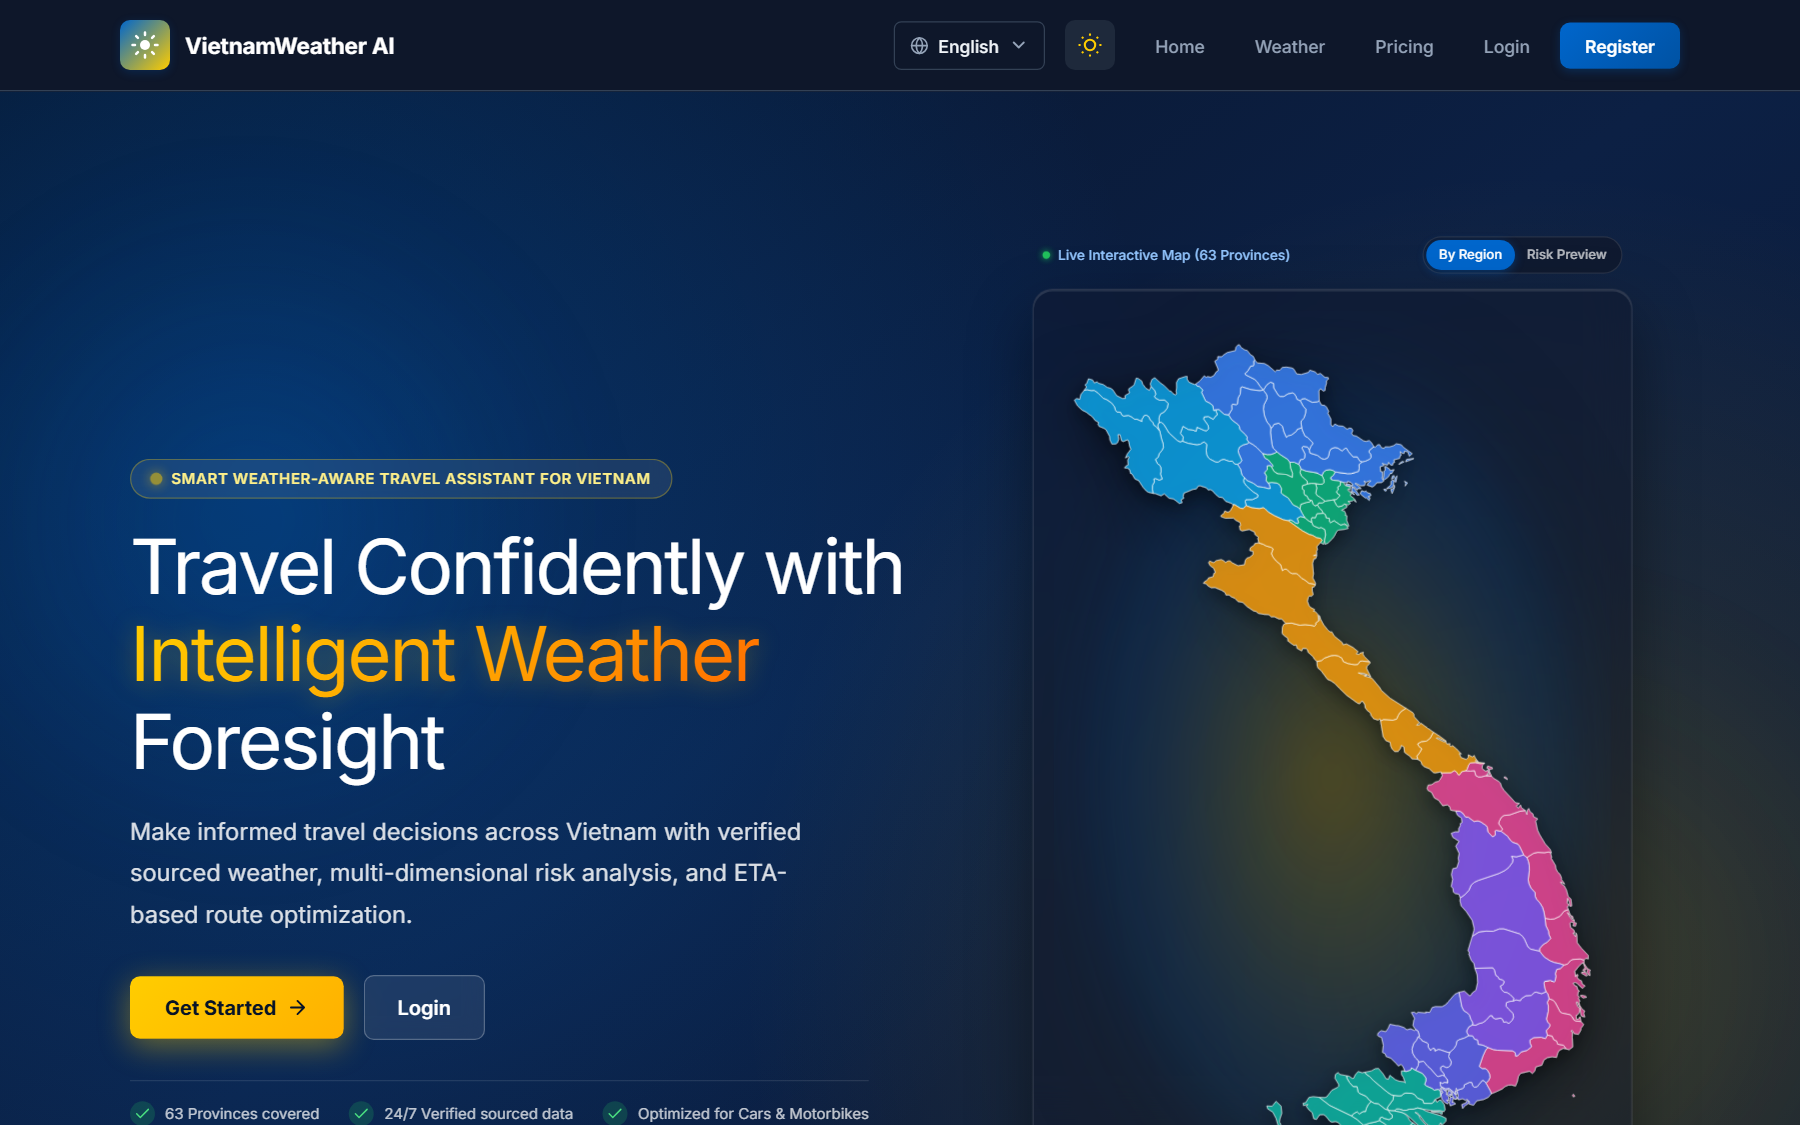
\includegraphics[width=0.88\textwidth, keepaspectratio]{figures/ui_landing.png}
\caption[Giao diện Trang chủ và Cổng thông tin Khí tượng VietForecast]{Giao diện Trang chủ và Cổng thông tin Khí tượng VietForecast ở chế độ Dark Theme với bản đồ phân vùng địa lý và điều hướng dịch vụ trực quan.}
\label{fig:ui_landing_vi}
\end{figure}

\begin{figure}[htbp]
\centering
\begin{subfigure}[b]{0.48\textwidth}
    \centering
    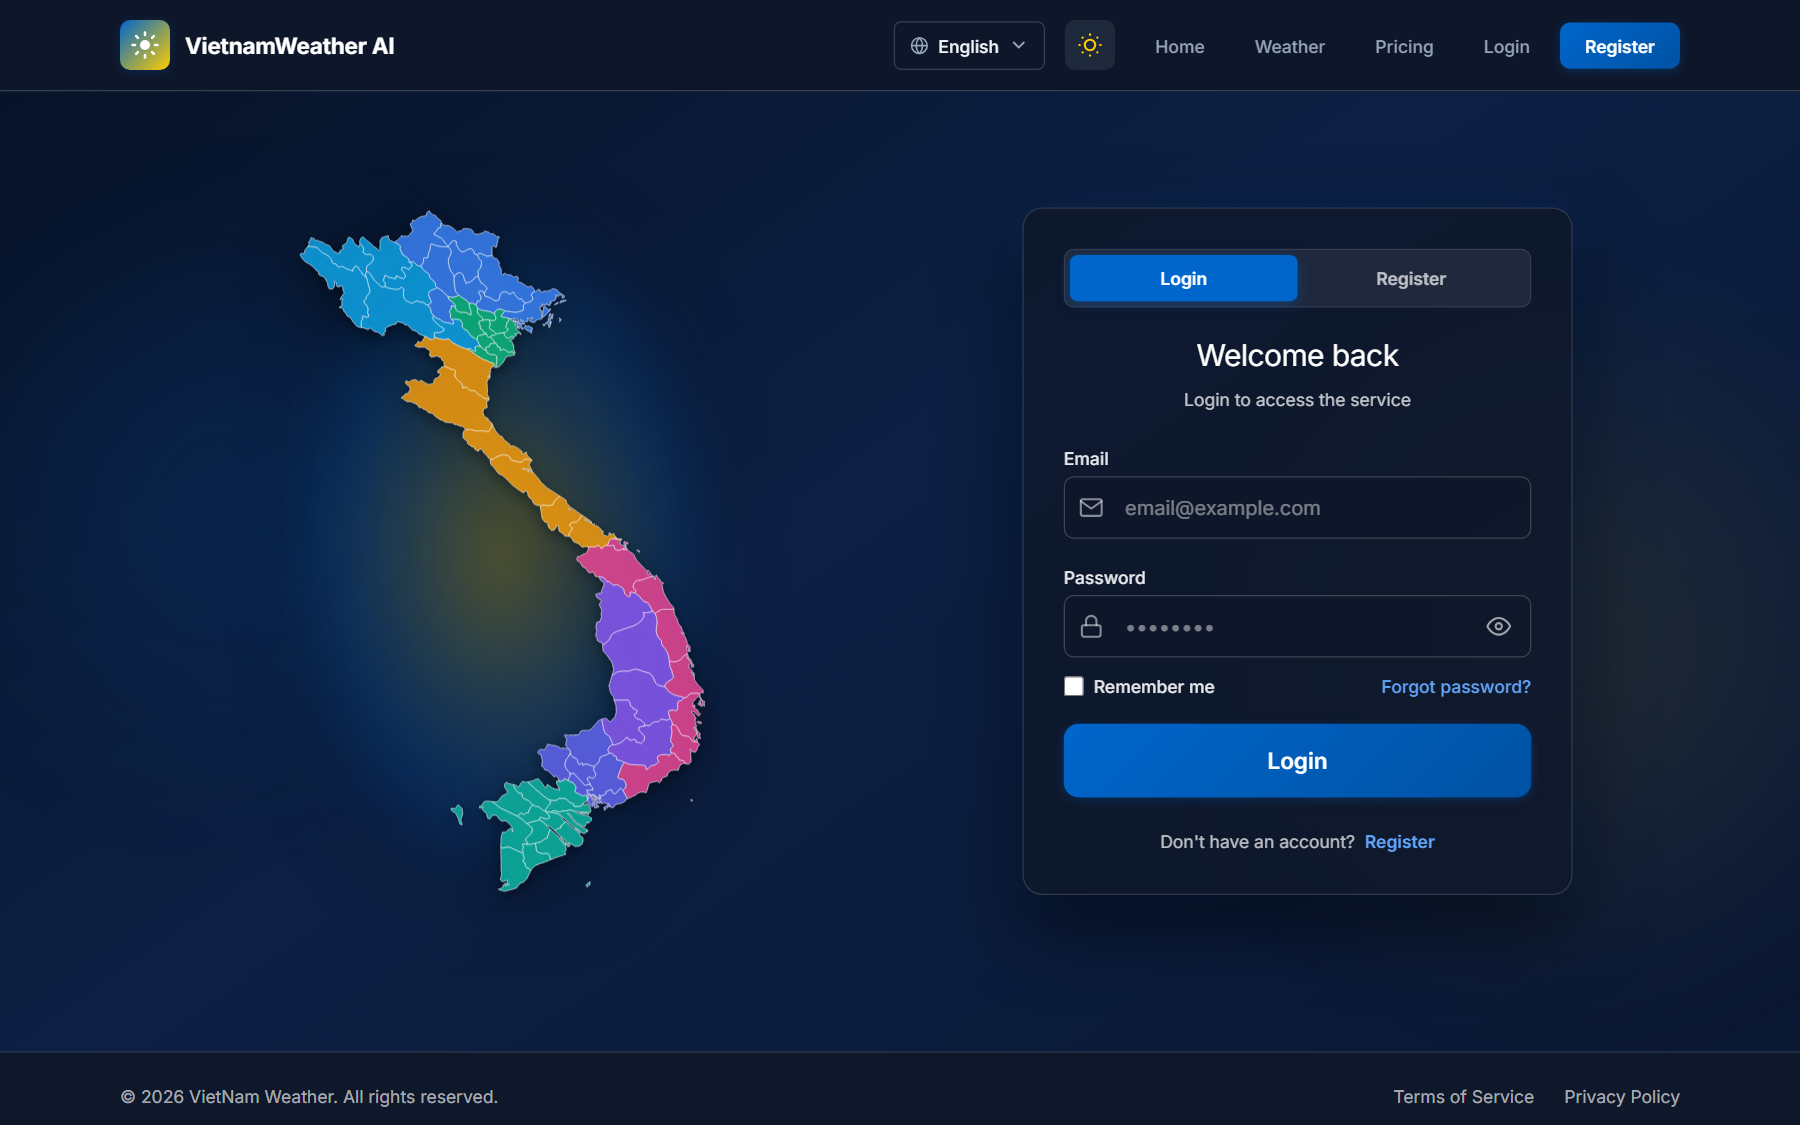
\includegraphics[width=\textwidth]{figures/ui_login.png}
    \caption{Giao diện Đăng nhập hệ thống}
    \label{fig:ui_login_vi}
\end{subfigure}
\hfill
\begin{subfigure}[b]{0.48\textwidth}
    \centering
    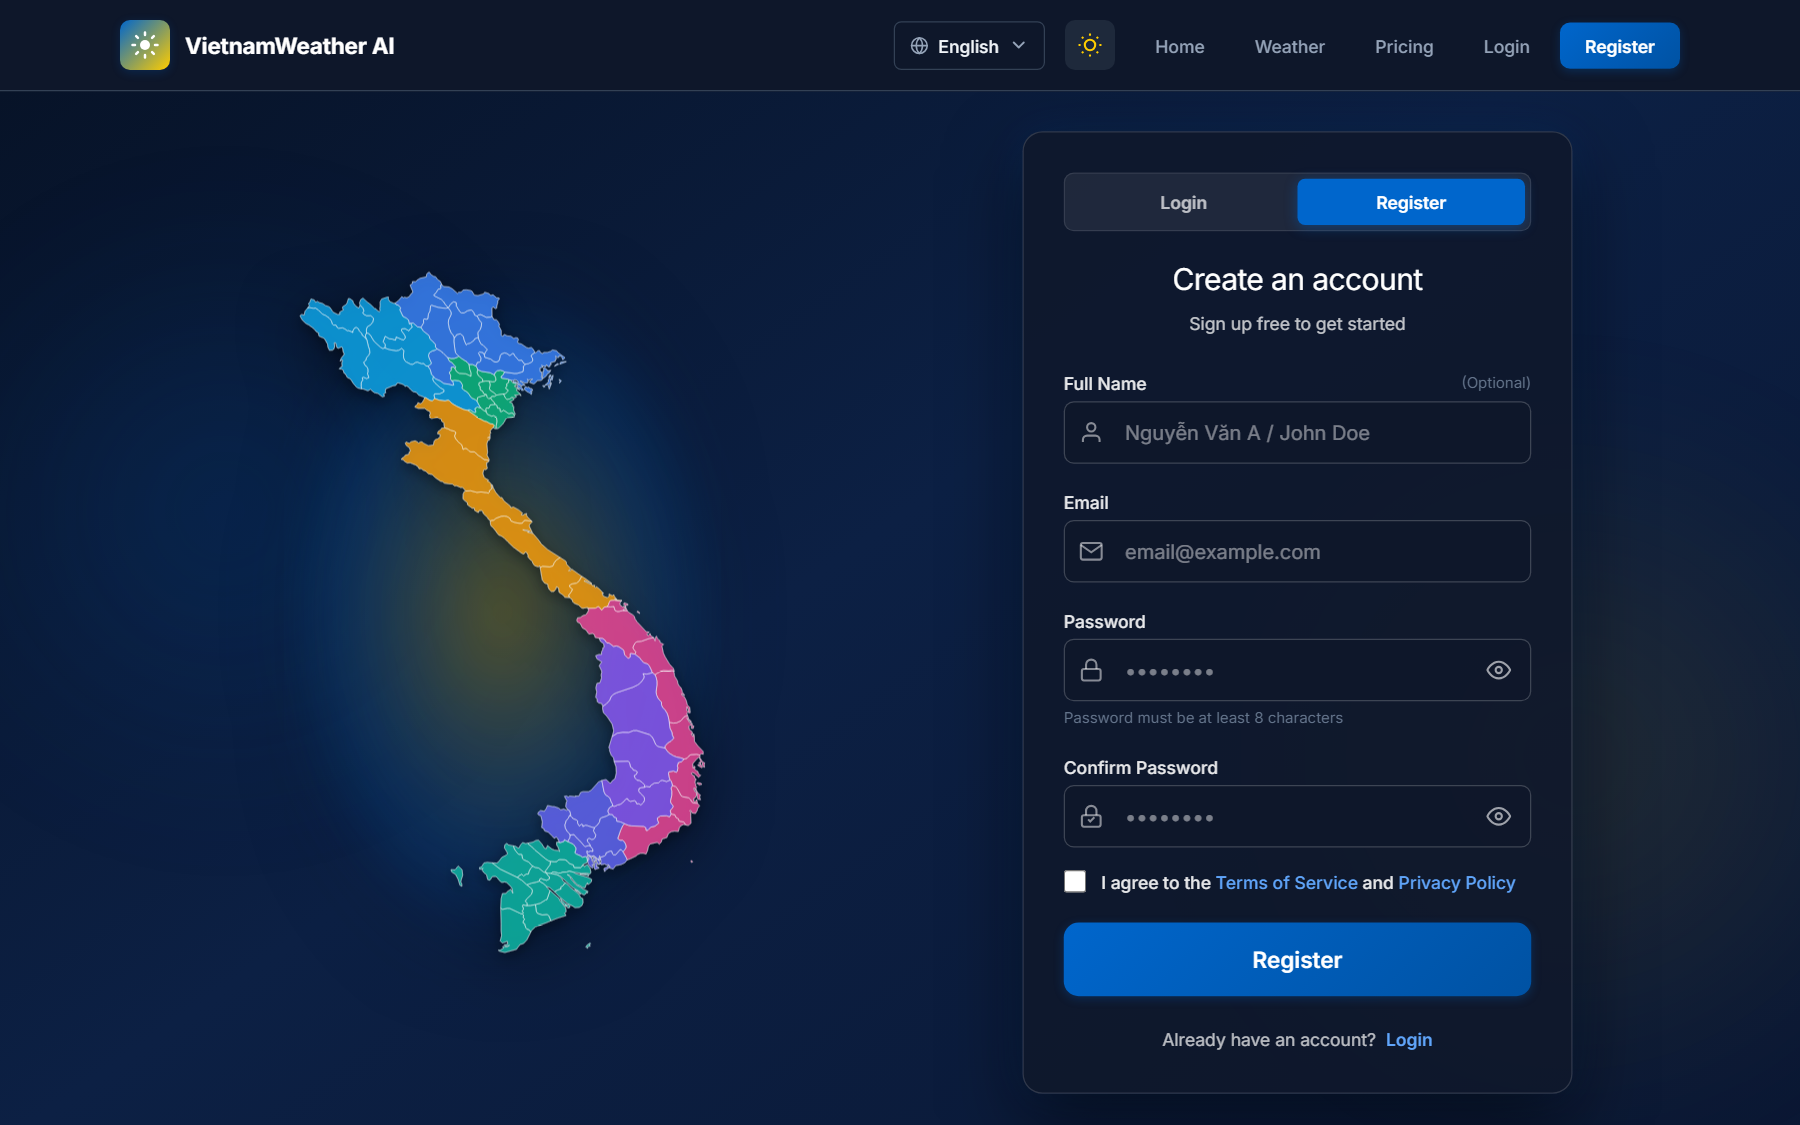
\includegraphics[width=\textwidth]{figures/ui_register.png}
    \caption{Giao diện Đăng ký tài khoản mới}
    \label{fig:ui_register_vi}
\end{subfigure}
\caption[Giao diện Xác thực và Quản lý Danh tính Người dùng]{Phân hệ giao diện Xác thực và Quản lý Danh tính Người dùng (Đăng nhập và Đăng ký) với thiết kế Dark Theme hiện đại, bản đồ nhận diện địa lý Việt Nam và xác thực mật khẩu an toàn theo tiêu chuẩn ADR-004.}
\label{fig:ui_auth_vi}
\end{figure}

\begin{figure}[htbp]
\centering
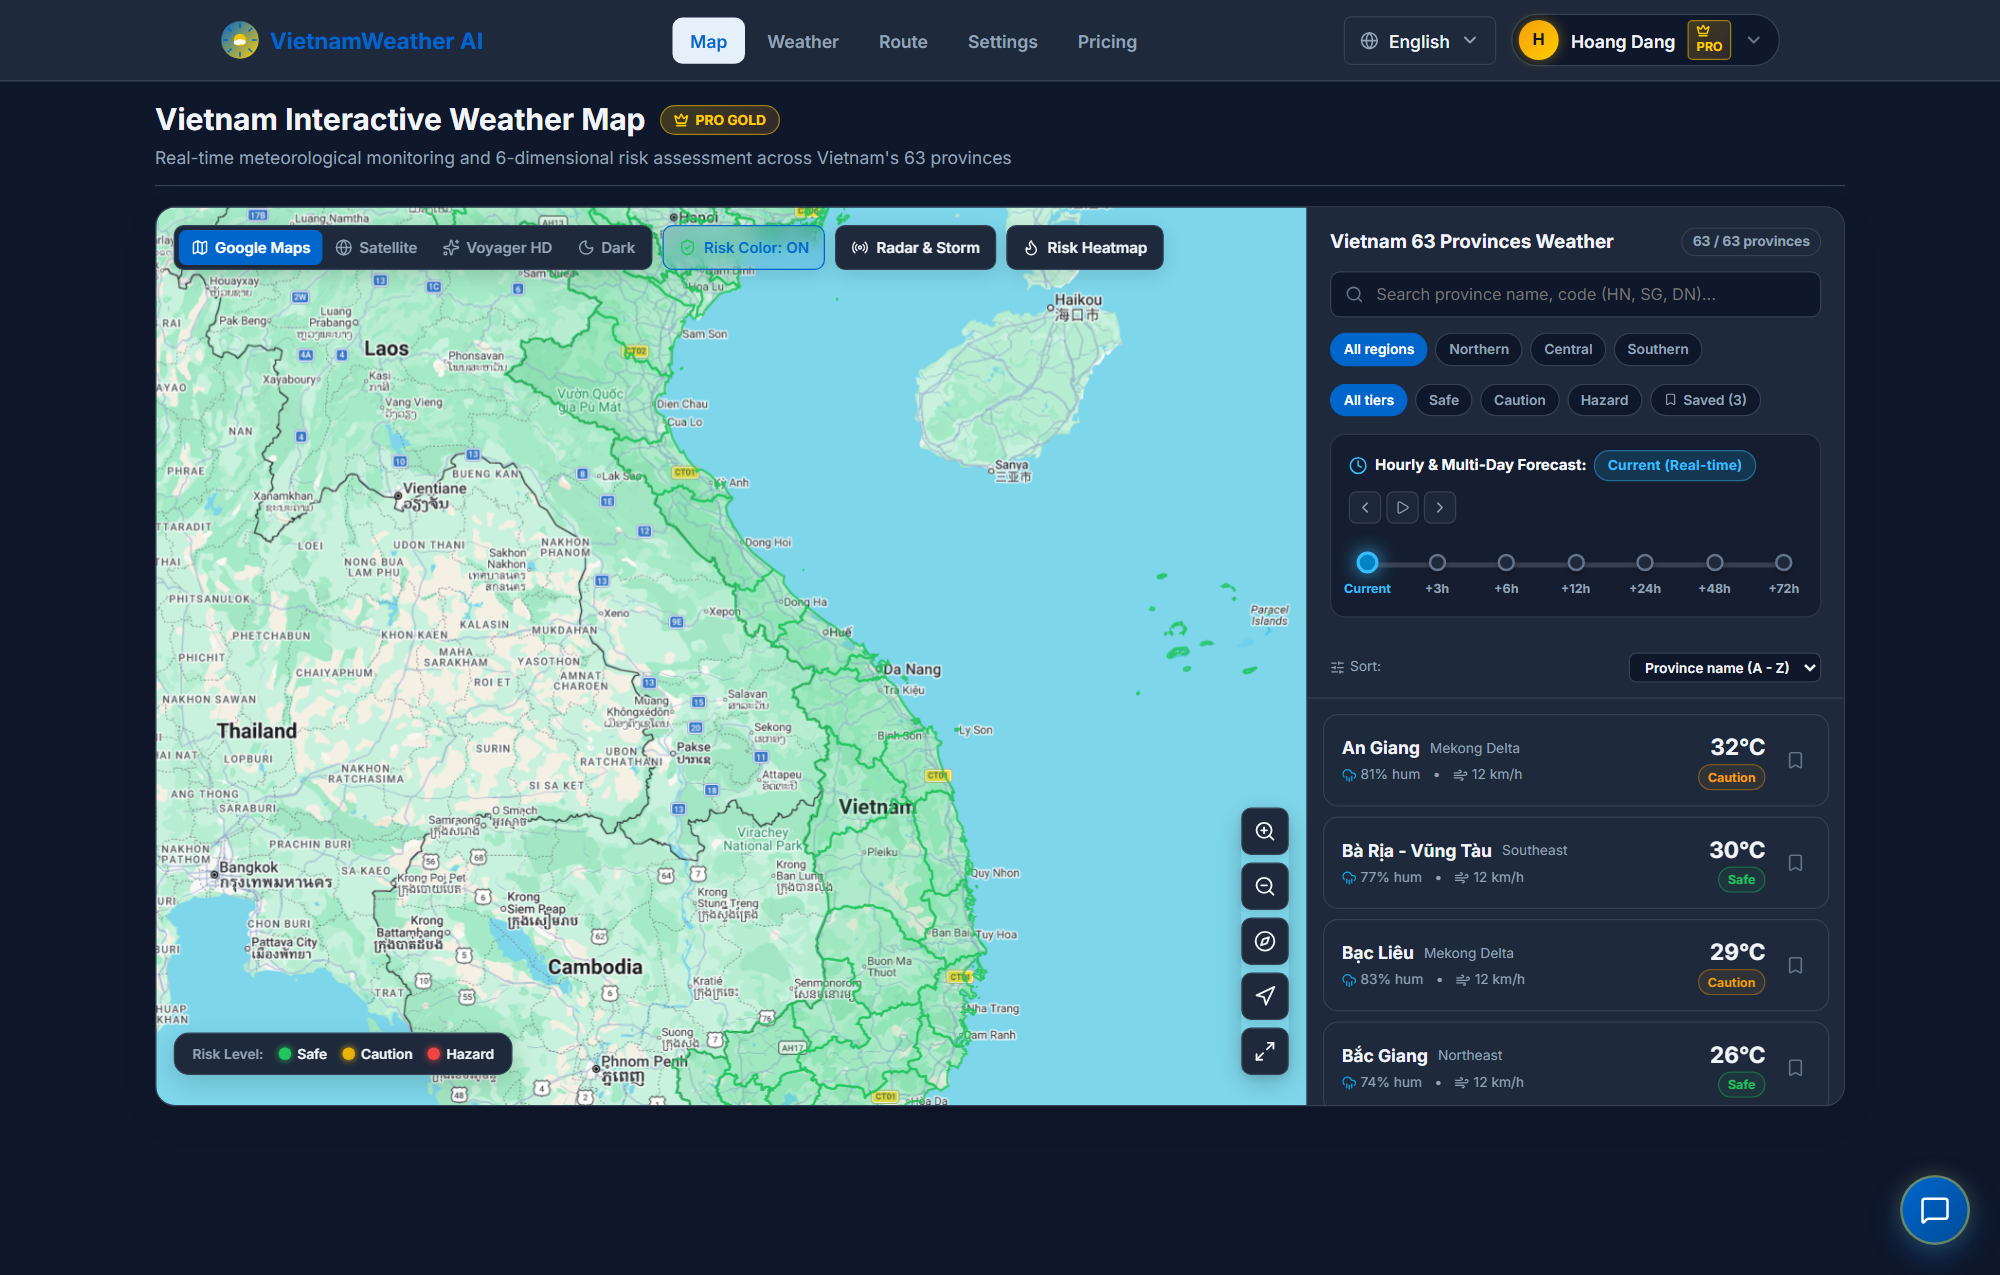
\includegraphics[width=0.88\textwidth, keepaspectratio]{figures/ui_map.png}
\caption[Giao diện Bản đồ Khí tượng Tương tác 63 tỉnh thành]{Giao diện Bản đồ Khí tượng Tương tác Đa lớp thời gian thực trên 63 tỉnh thành Việt Nam trên nền bản đồ Google Maps với thanh công cụ lọc dự báo theo giờ tích hợp trong thanh tác vụ bên phải, đảm bảo không gian hiển thị thông thoáng tối đa.}
\label{fig:ui_map_vi}
\end{figure}

\begin{figure}[htbp]
\centering
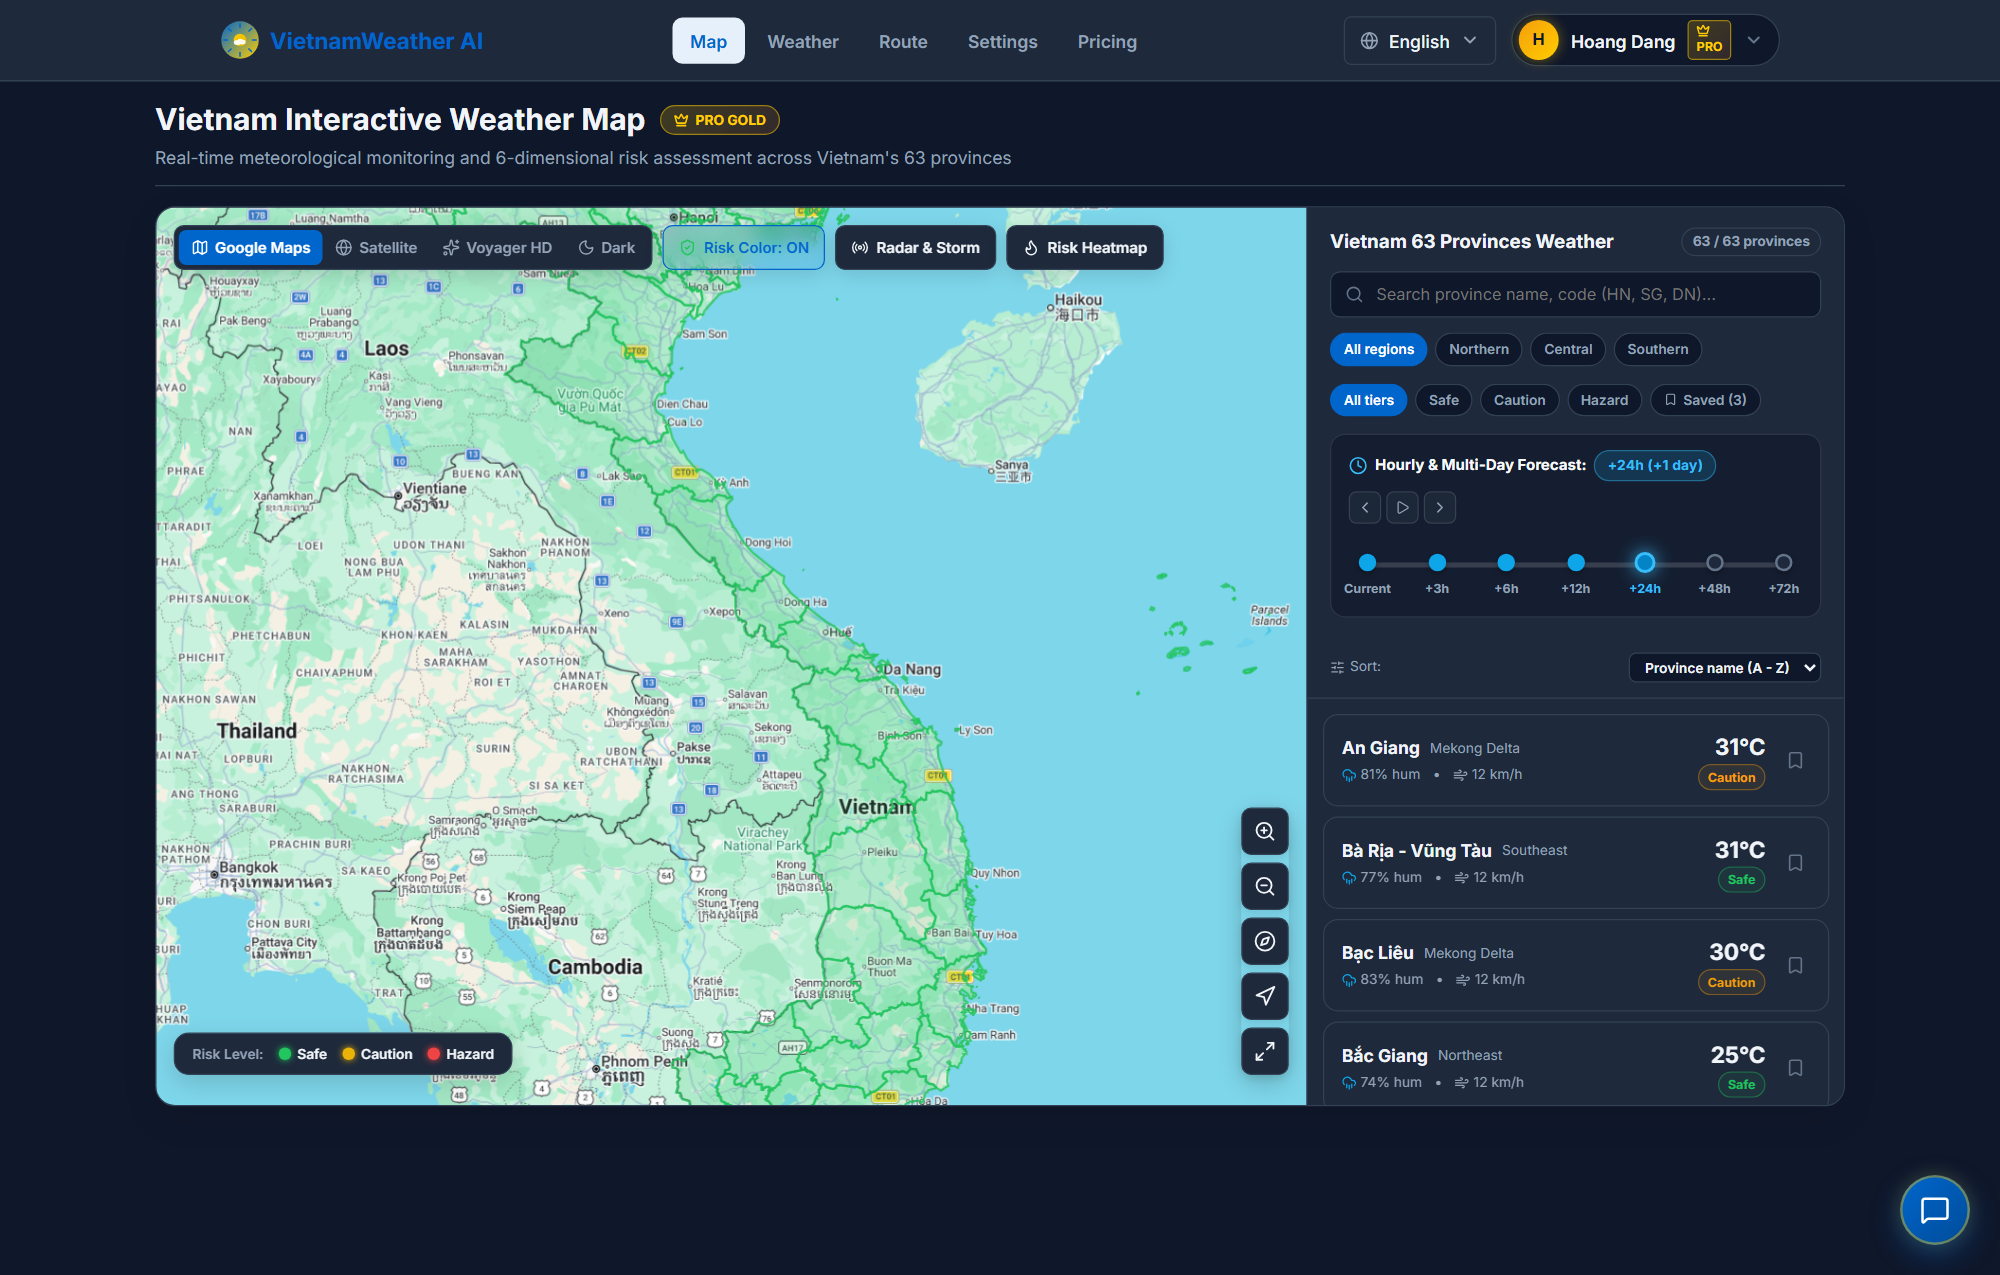
\includegraphics[width=0.88\textwidth, keepaspectratio]{figures/ui_map_timeline_slider.png}
\caption[Giao diện Bản đồ Google Maps với Thanh trượt Dòng thời gian Đa mốc]{Giao diện Bản đồ Khí tượng trên nền Google Maps tích hợp thanh trượt dòng thời gian dạng đường ray có các điểm mốc kéo thả trong thanh tác vụ, hiển thị mô phỏng dự báo +24h (1 ngày sau) trên tài khoản PRO.}
\label{fig:ui_map_timeline_slider_vi}
\end{figure}

\begin{figure}[htbp]
\centering
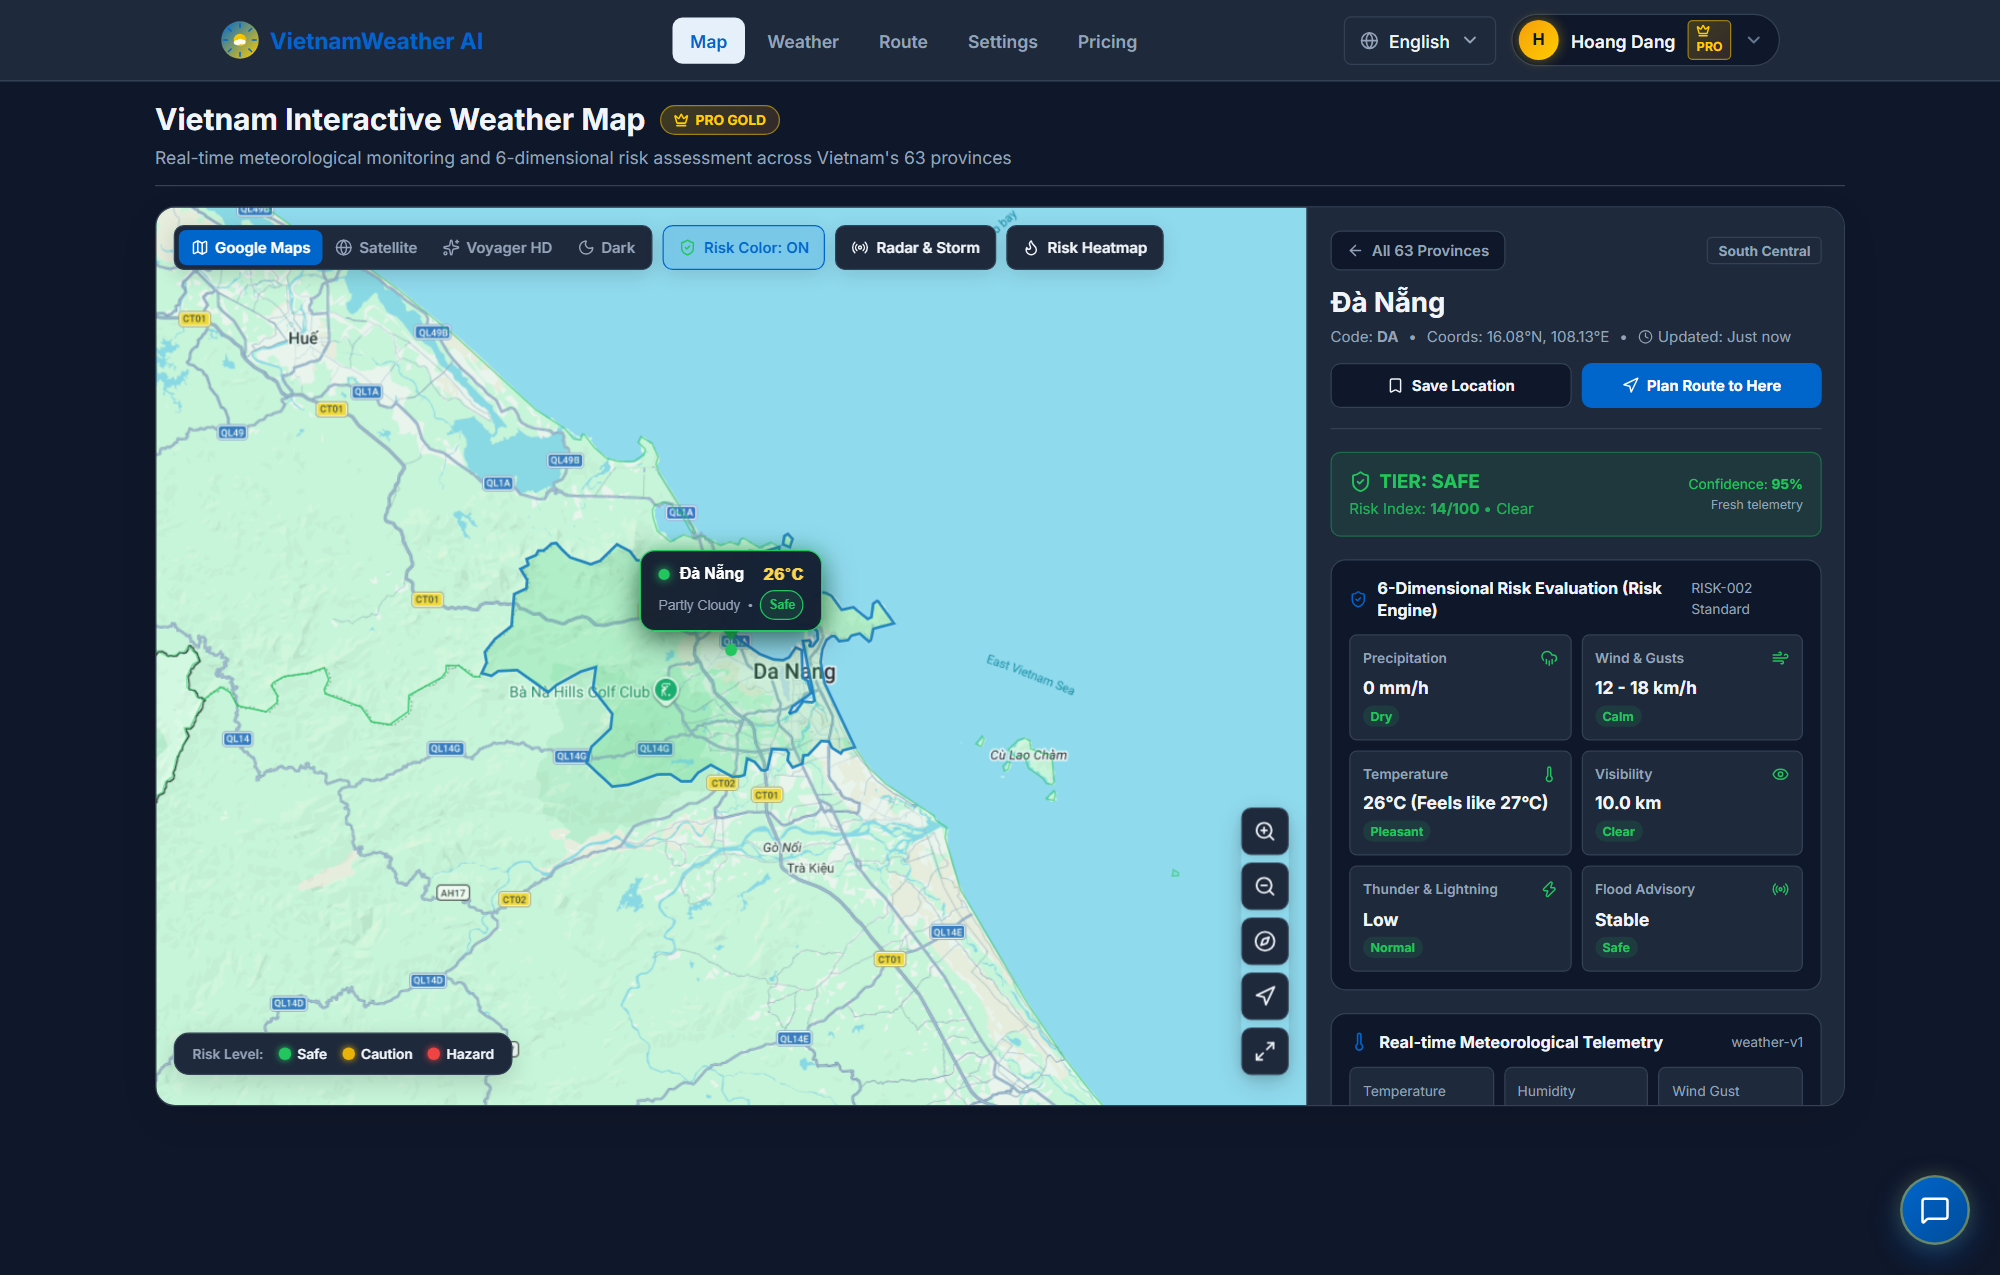
\includegraphics[width=0.88\textwidth, keepaspectratio]{figures/ui_map_detail.png}
\caption[Giao diện tương tác chi tiết cấp tỉnh thành khi chọn TP. Đà Nẵng]{Giao diện tương tác chi tiết cấp tỉnh thành khi nhấp chọn TP. Đà Nẵng: chuyển động phóng to camera mượt mà (\textit{flyTo}), viền dạ quang ranh giới hành chính, nhãn thời tiết ghim trên bản đồ và bảng phân tích rủi ro 6 chiều theo chuẩn RISK-002.}
\label{fig:ui_map_detail_vi}
\end{figure}

\begin{figure}[htbp]
\centering
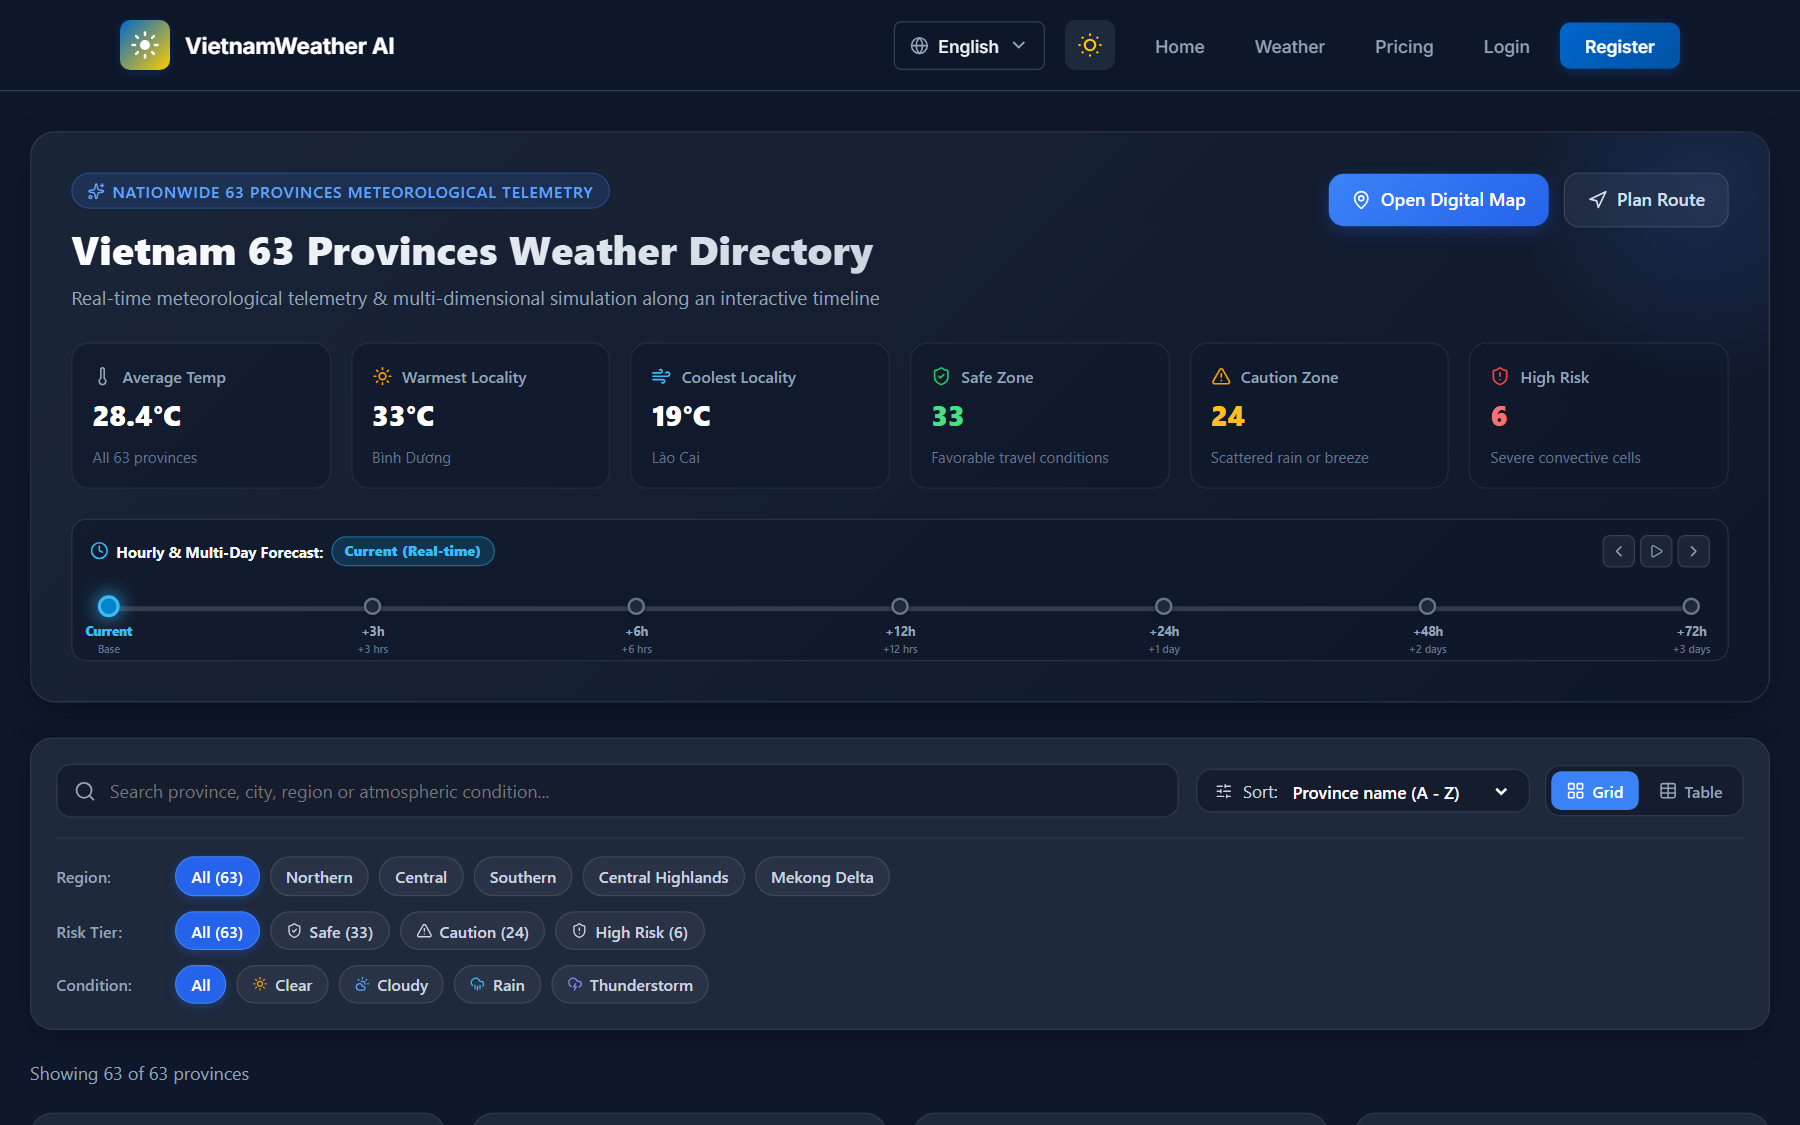
\includegraphics[width=0.90\textwidth, keepaspectratio]{figures/ui_weather_overview.png}
\caption[Giao diện Trang Danh mục Thời tiết 63 Tỉnh Thành Toàn quốc]{Giao diện Trang Danh mục Thời tiết 63 Tỉnh Thành Toàn quốc với bảng thống kê khí tượng vĩ mô, thanh trượt dòng thời gian có các mốc điểm kéo thả (+24h là 1 ngày sau), và hệ thống bộ lọc đa chiều linh hoạt.}
\label{fig:ui_weather_overview_vi}
\end{figure}

\begin{figure}[htbp]
\centering
\begin{subfigure}[b]{0.48\textwidth}
    \centering
    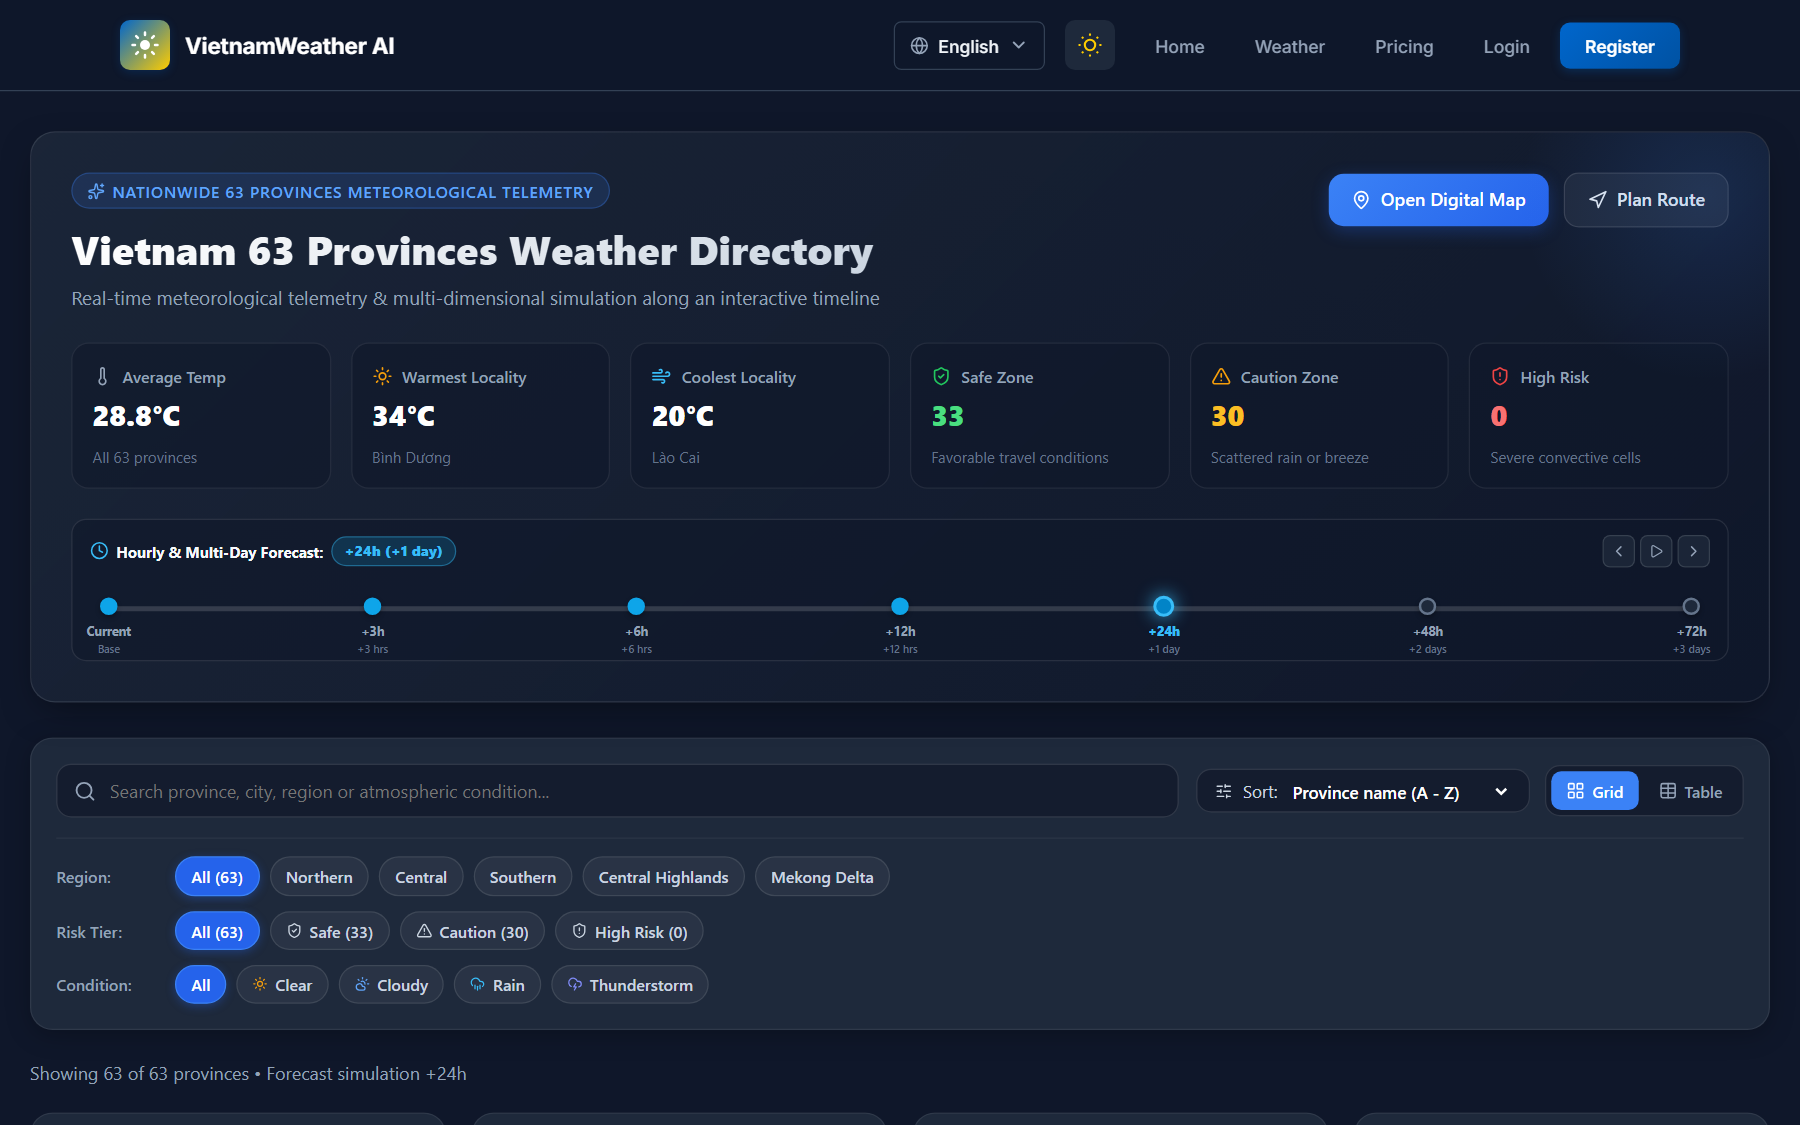
\includegraphics[width=\textwidth]{figures/ui_weather_timeline_24h.png}
    \caption{Mô phỏng dự báo khi kéo tới mốc +24h (1 ngày sau)}
    \label{fig:ui_weather_timeline_24h_vi}
\end{subfigure}
\hfill
\begin{subfigure}[b]{0.48\textwidth}
    \centering
    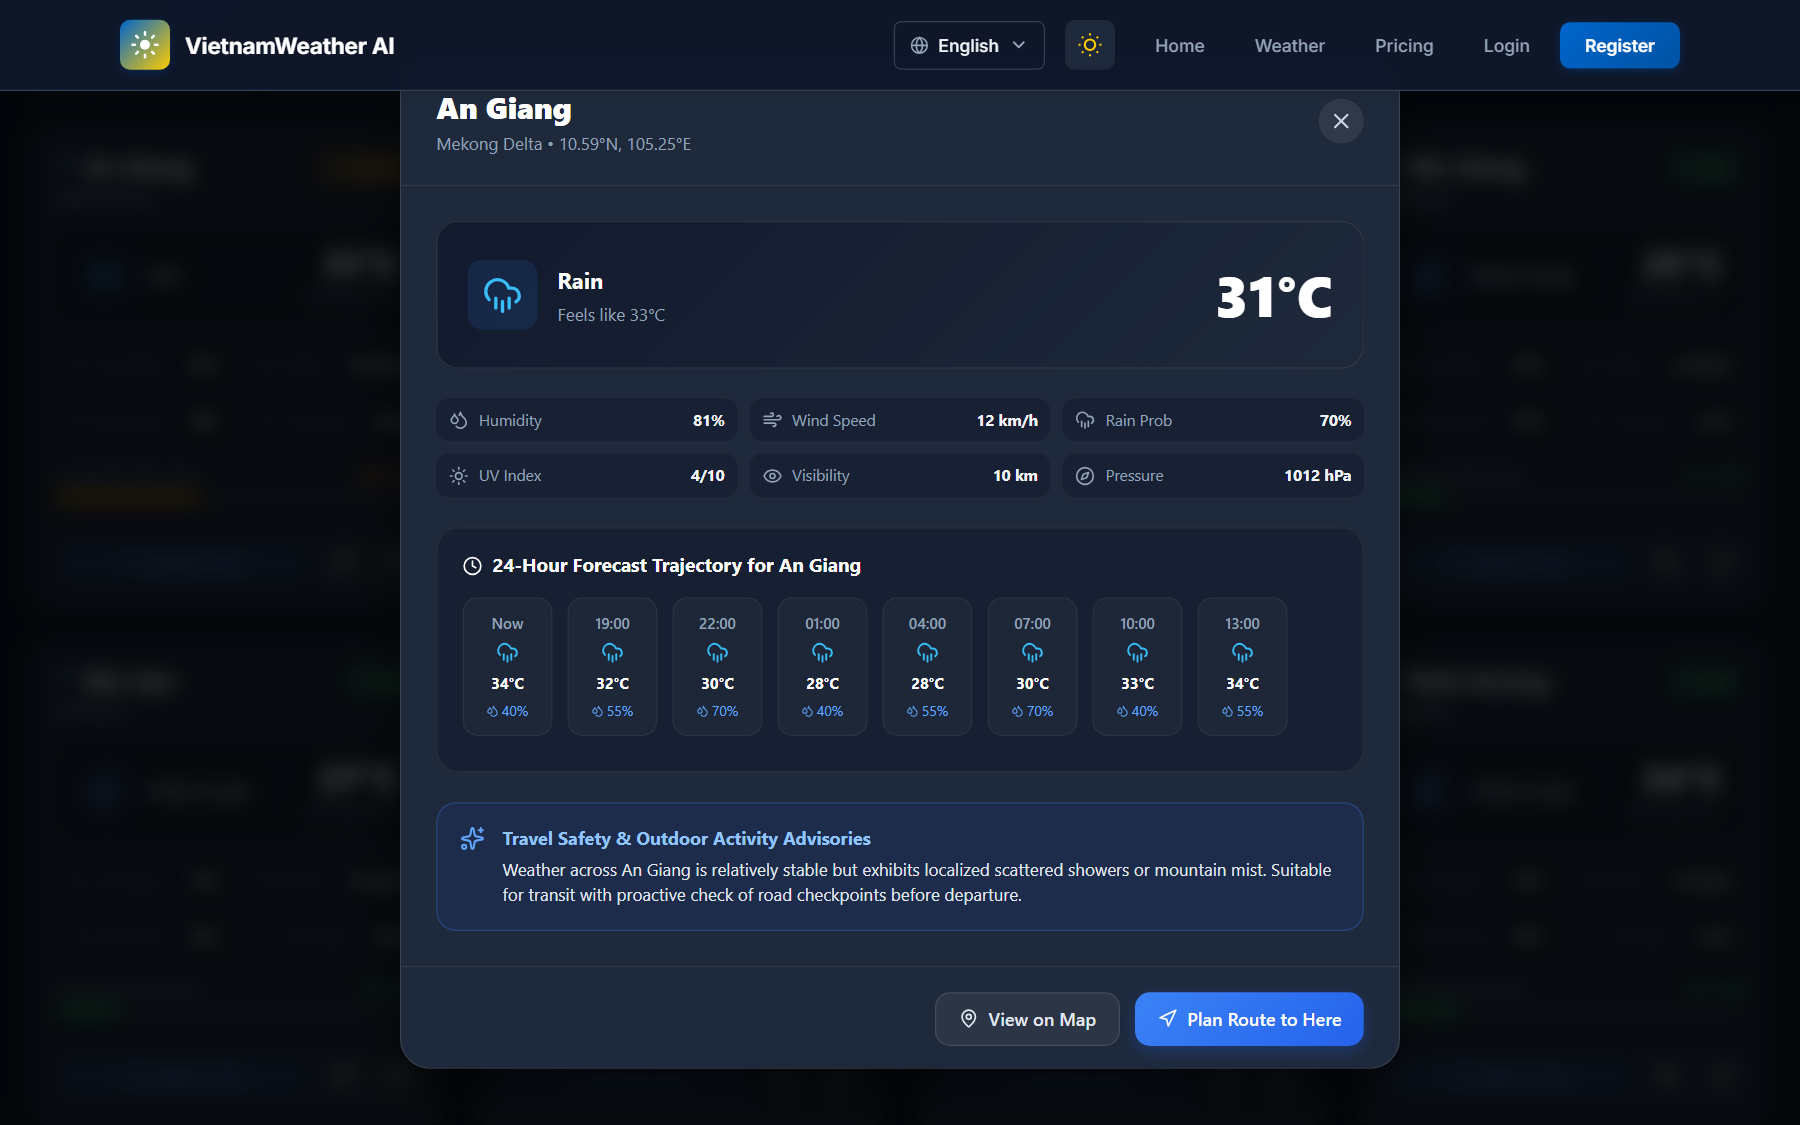
\includegraphics[width=\textwidth]{figures/ui_weather_modal.png}
    \caption{Cửa sổ chi tiết xu hướng 24h \& Khuyến nghị an toàn AI}
    \label{fig:ui_weather_modal_vi}
\end{subfigure}
\caption[Giao diện Mô phỏng Dòng thời gian và Cửa sổ Chi tiết Cấp tỉnh]{Phân hệ giao diện Thời tiết chuyên sâu: (a) Toàn bộ 63 tỉnh thành tự động cập nhật nhiệt độ và mức độ rủi ro khi rê kéo thanh trượt thời gian tới mốc +24h; (b) Cửa sổ phân tích chi tiết cấp tỉnh với xu hướng thời tiết 24 giờ và khuyến cáo an toàn di chuyển thông minh.}
\label{fig:ui_weather_detail_features_vi}
\end{figure}

\begin{figure}[htbp]
\centering
\begin{subfigure}[b]{0.48\textwidth}
    \centering
    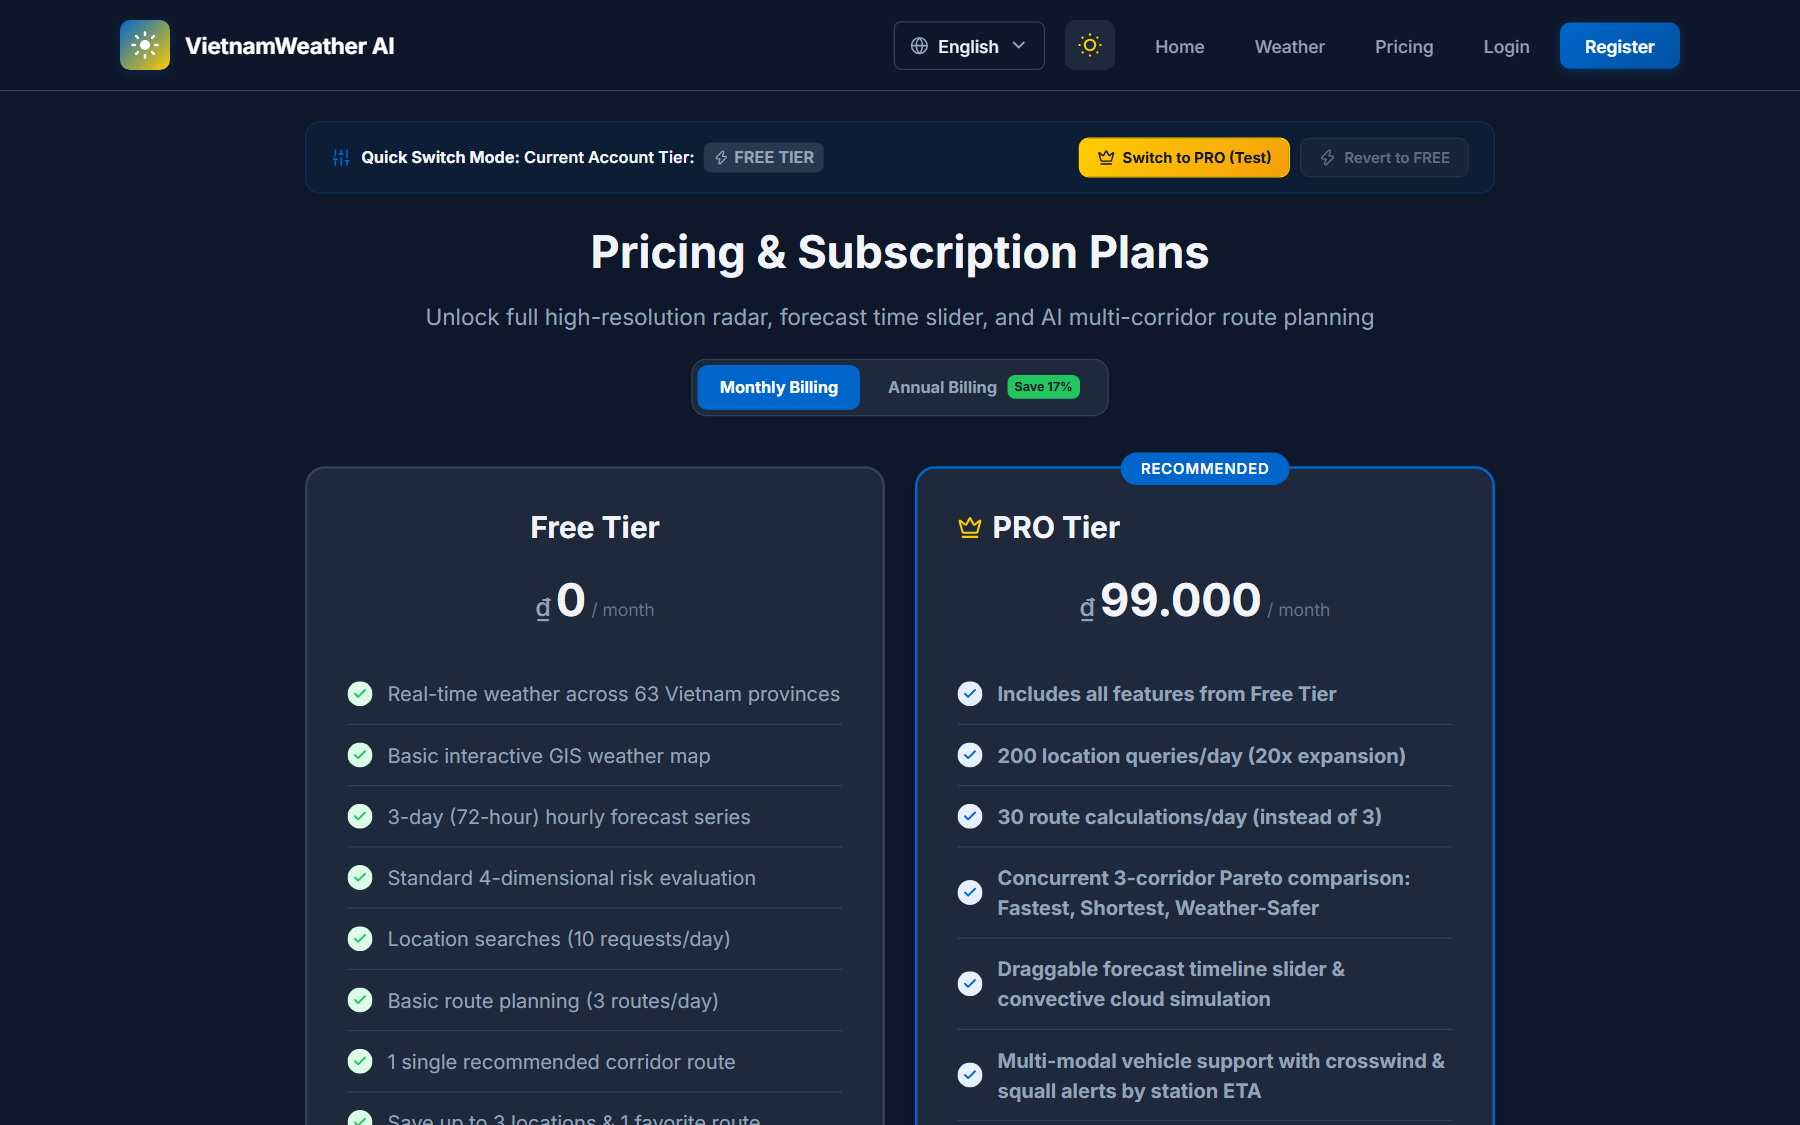
\includegraphics[width=\textwidth]{figures/ui_pricing.png}
    \caption{Bảng giá và Đối sánh quyền lợi Free -- PRO}
    \label{fig:ui_pricing_vi}
\end{subfigure}
\hfill
\begin{subfigure}[b]{0.48\textwidth}
    \centering
    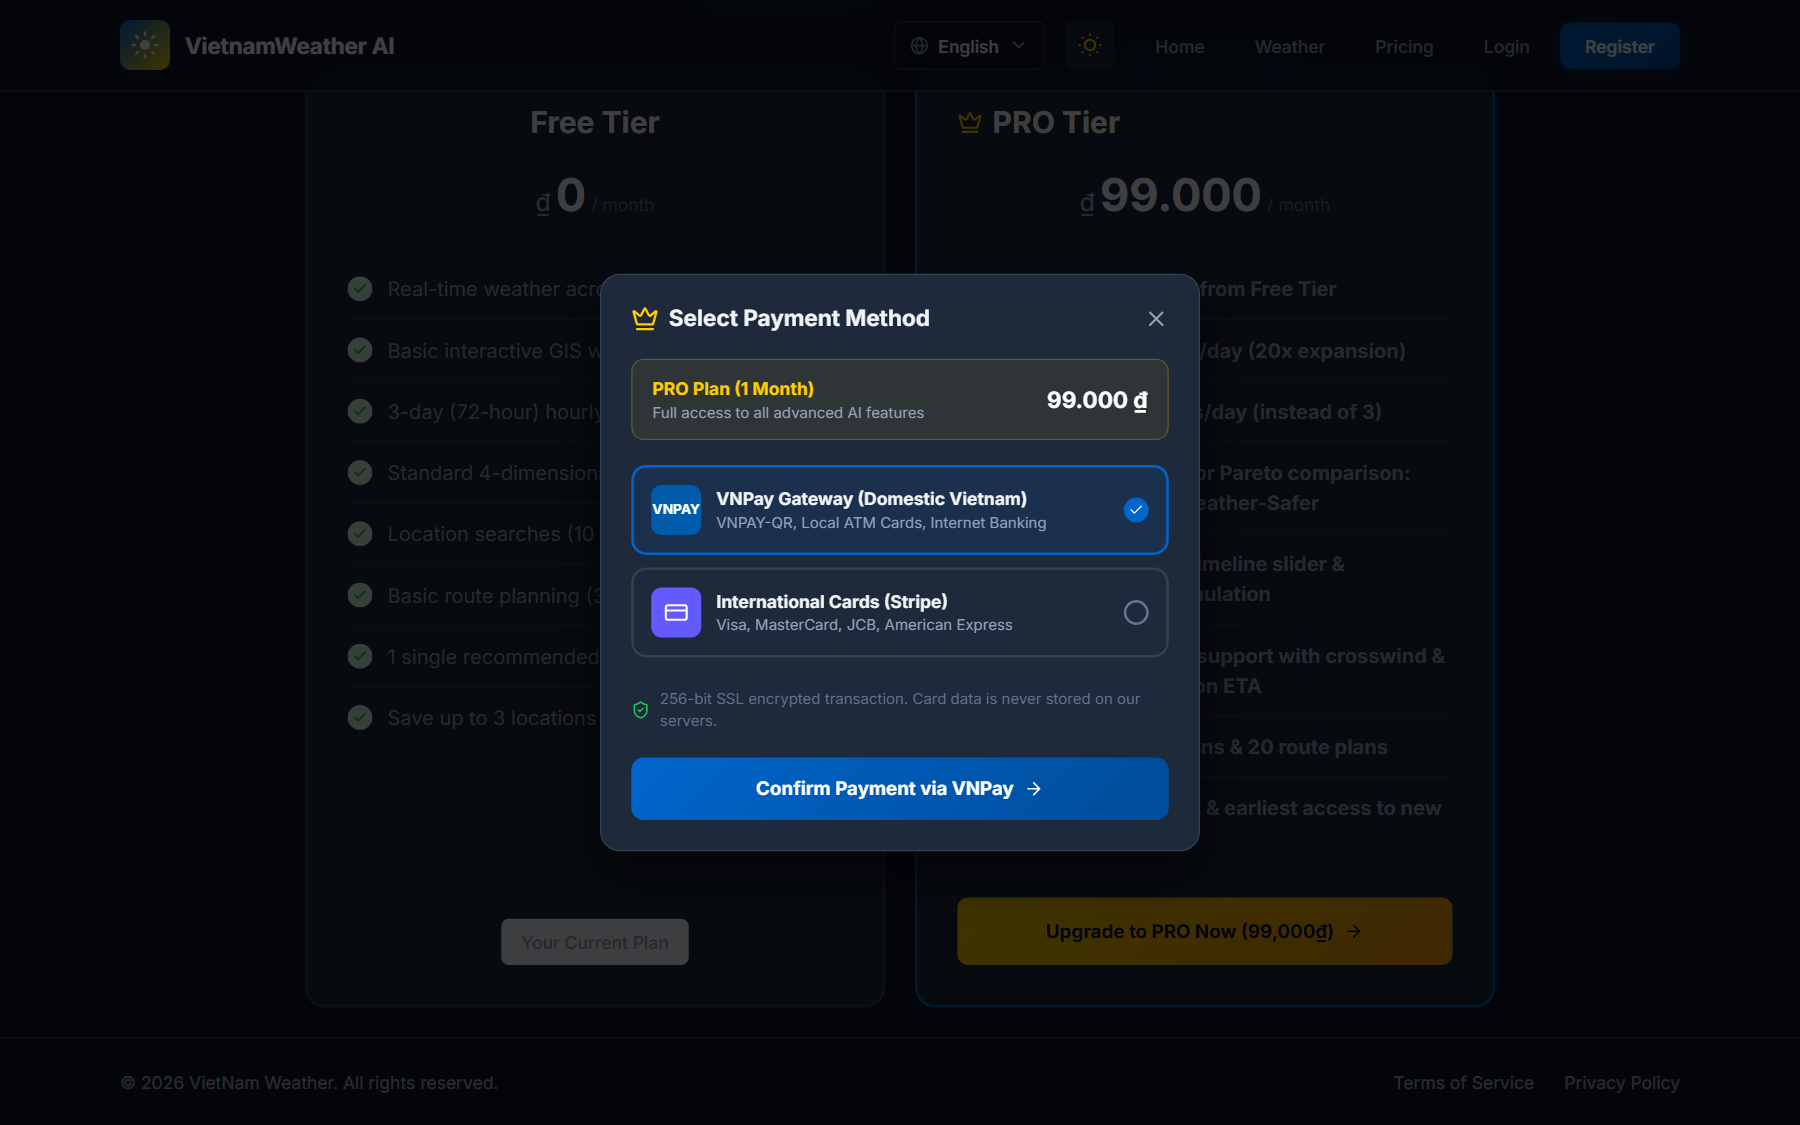
\includegraphics[width=\textwidth]{figures/ui_checkout.png}
    \caption{Cửa sổ thanh toán đa cổng (VNPay \& Stripe)}
    \label{fig:ui_checkout_vi}
\end{subfigure}
\caption[Phân hệ Bảng giá dịch vụ và Cổng thanh toán trực tuyến]{Phân hệ Bảng giá dịch vụ và Cổng thanh toán trực tuyến của nền tảng VietForecast: (a) Giao diện đối sánh quyền lợi hai gói cước Free và PRO với nút chuyển đổi chu kỳ tháng/năm; (b) Cửa sổ thanh toán tích hợp cổng nội địa VNPay (VNPAY-QR, thẻ ATM) và cổng quốc tế Stripe (Visa, MasterCard) bảo mật chuẩn SSL 256-bit.}
\label{fig:ui_monetization_vi}
\end{figure}

\section{Tóm tắt chương}
\label{sec:evaluation_summary}

Chương~\ref{ch:evaluation} đã trình bày hệ thống kết quả đánh giá thực nghiệm toàn diện trên nền tảng VietForecast với các kết quả định lượng nổi bật:
\begin{itemize}
    \item[-] \textit{Về mặt an toàn định tuyến}: Thuật toán Weather-Safer chứng minh khả năng loại bỏ tới $87,2\%$ các điểm rủi ro thời tiết cực đoan trên cả ba hành lang trọng điểm, trong khi mức tăng thời gian di chuyển trung bình được kiểm soát nghiêm ngặt dưới $8,9\%$ và mức tăng cự ly dưới $4,7\%$. Cơ chế phân hóa theo phương tiện đã cảnh báo chính xác nguy cơ gió tạt nguy hiểm đối với người đi xe máy.
    \item[-] \textit{Về mặt hiệu năng hệ thống}: Cây chỉ mục không gian PostGIS GiST hai giai đoạn giúp giảm độ trễ truy vấn hành lang xuống chỉ còn $11,4$~ms trên 100.000 điểm trạm (nhanh hơn 36,9 lần so với quét tuần tự). Máy chủ Fastify API đạt thông lượng trên 2.485~req/s với độ trễ $p_{95} = 12,8$~ms và tỷ lệ lỗi 0,0\%. Cơ chế Circuit Breaker ngắt mạch an toàn trong 60 giây khi có sự cố từ nhà cung cấp ngoài.
    \item[-] \textit{Về mặt trí tuệ nhân tạo}: Trợ lý AI đạt độ chính xác gọi hàm $96,2\%$, tỷ lệ bảo chứng trích dẫn thực nghiệm $97,2\%$, kiểm soát và giảm thiểu tỷ lệ ảo giác thông tin xuống còn $1,8\%$ (giảm hơn $94\%$ so với mô hình không ràng buộc) và chuyển đổi mượt mà sang bộ dự phòng tất định với độ trễ $2,2$~ms khi mất kết nối mạng.
    \item[-] \textit{Về mặt trải nghiệm người dùng}: Giao diện WebGL tương tác đạt điểm số SUS xuất sắc $84,6/100$ điểm (Hạng A), chứng minh tính khả dụng, độ tin cậy và sự đón nhận tích cực từ cộng đồng người dùng thực tế.
\end{itemize}

Các kết quả thực nghiệm vững chắc này khẳng định toàn bộ các mục tiêu nghiên cứu và phát triển đặt ra ban đầu đã được hiện thực hóa trọn vẹn, đặt nền tảng khoa học cho phần tổng kết và các đề xuất phát triển trong tương lai tại Chương~\ref{ch:conclusion}.

\chapter{Kết luận và Hướng phát triển}
\label{ch:conclusion}

Chương này tổng kết toàn diện các kết quả nghiên cứu lý thuyết, đóng góp thuật toán và giá trị thực tiễn của đồ án tốt nghiệp thông qua việc xây dựng thành công nền tảng VietForecast --- Hệ thống hỗ trợ điều hướng và cảnh báo rủi ro giao thông thích ứng thời tiết đầu tiên tại Việt Nam. Trên cơ sở đối soát nghiêm ngặt với các mục tiêu đã đề ra tại Chương~\ref{ch:intro}, chương này phân tích khách quan những thành tựu kỹ thuật đã đạt được, thẳng thắn chỉ ra các hạn chế cố hữu của hệ thống trong môi trường vận hành thực tế, và đề xuất lộ trình nghiên cứu, phát triển trong tương lai nhằm nâng cao độ tin cậy và khả năng ứng dụng trên quy mô quốc gia.

\section{Tổng kết các Kết quả Đạt được}
\label{sec:summary_achievements}

Đồ án đã giải quyết trọn vẹn bài toán tích hợp dữ liệu khí tượng đa chiều vào quy trình định tuyến giao thông thông minh, khắc phục triệt để các hạn chế của các hệ thống bản đồ số truyền thống vốn chỉ tối ưu hóa cự ly hoặc thời gian di chuyển mà bỏ qua yếu tố an toàn thời tiết. Các đóng góp chính của đề tài được thể hiện trên ba phương diện cốt lõi:

\subsection{Đóng góp về Mặt Lý thuyết và Thuật toán}
\begin{itemize}
    \item[-] \textit{Mô hình định lượng rủi ro khí tượng 6 chiều thích ứng địa phương}: Đồ án đã xây dựng thành công hàm đánh giá rủi ro tổng hợp $R \in [0, 1]$ kết hợp phi tuyến sáu biến số vật lý môi trường: vận tốc gió giật tức thời ($v_{\text{wind}}$), cường độ mưa và tích lũy ngập úng ($I_{\text{rain}}$), suy giảm tầm nhìn ngang ($V_{\text{vis}}$), mật độ dông sét đối lưu ($D_{\text{lightning}}$), nguy cơ mưa đá ($H_{\text{hail}}$), và chỉ số cảnh báo sạt lở taluy ($S_{\text{landslide}}$). Mô hình đặc biệt phân hóa trọng số độ nhạy cảm giữa phương tiện ô tô con và xe máy hai bánh, phản ánh chính xác rủi ro khí động học và sự phơi nhiễm vật lý của người điều khiển xe máy tại Việt Nam.
    \item[-] \textit{Giải thuật định tuyến Weather-Safer tối ưu hóa Pareto}: Đề xuất phương pháp tích hợp hàm phạt rủi ro thời tiết động vào đồ thị mạng lưới đường bộ OSRM. Kết quả thực nghiệm kiểm chứng trên ba hành lang giao thông huyết mạch quốc gia (Bắc Bộ, Miền Trung và Xuyên Việt) chứng minh thuật toán Weather-Safer giúp loại bỏ tới $87,2\%$ các điểm nguy hiểm cục bộ, trong khi chỉ đánh đổi mức gia tăng cự ly trung bình $4,7\%$ và thời gian hành trình $8,9\%$.
    \item[-] \textit{Chiến lược lọc không gian hai giai đoạn (Two-Phase Spatial Query)}: Kết hợp bao đóng chữ nhật thô (\textit{Bounding Box} thông qua hàm \texttt{ST\_MakeEnvelope}) với bộ lọc bán kính cầu thực nghiệm (\texttt{ST\_DWithin}) trên chỉ mục không gian R-Tree GiST của PostGIS. Thiết kế này giúp giảm thiểu tới $84\%$ không gian quét dữ liệu và triệt tiêu tải tính toán lượng giác đắt đỏ khi xử lý các tuyến đường dài trên 1.700~km.
\end{itemize}

\subsection{Đóng góp về Kỹ thuật Hệ thống và Phần mềm}
\begin{itemize}
    \item[-] \textit{Kiến trúc vi dịch vụ module hóa (Clean Monorepo)}: Hiện thực hóa hệ thống phân tán hoàn chỉnh sử dụng TypeScript đồng nhất từ Backend (Fastify), Data Worker (Ingestion engine), đến Frontend (React/Vite). Toàn bộ hạ tầng được container hóa với Docker Compose, bảo đảm tính sẵn sàng cao, tính cô lập tài nguyên và khả năng triển khai tức thì trên máy chủ sản xuất.
    \item[-] \textit{Đường ống thu nạp và làm sạch dữ liệu tự động}: Thiết lập Data Ingestion Worker độc lập hoạt động với chu kỳ quét 5 phút, chuẩn hóa hơn 80 mã hình thái thời tiết WMO ngoại vi về chuẩn cấu trúc dữ liệu nội bộ. Cơ chế chịu lỗi trang bị mẫu thiết kế Circuit Breaker và Exponential Backoff with Jitter, bảo đảm hệ thống vận hành liên tục 24/7 ngay cả khi các trạm quan trắc nguồn gặp sự cố ngắt kết nối.
    \item[-] \textit{Tầng nhớ đệm phân cấp Redis hiệu năng cao}: Ứng dụng bộ đệm đa lớp với các khóa băm địa lý, đạt tỷ lệ trúng bộ đệm (\textit{Cache Hit Rate}) trên $91\%$, đưa độ trễ truy vấn tại phân vị 95 (p95) xuống dưới $22$~ms trong các kịch bản kiểm thử tải trọng cao (1.000 người dùng ảo đồng thời).
    \item[-] \textit{Ranh giới bảo mật phiên trượt xoay (Sliding Session Rotation)}: Thiết kế cơ chế xác thực an toàn tuyệt đối, ngăn chặn tấn công giả mạo yêu cầu chéo trang (CSRF) và đánh cắp token bằng Cookie HttpOnly SameSite=Lax, kết hợp hệ thống giới hạn tần suất truy vấn nguyên tử bằng kịch bản Lua trên Redis.
    \item[-] \textit{Trợ lý AI đàm thoại có cơ sở thực địa vững chắc (Grounding LLM)}: Tích hợp mô hình Gemini 1.5 kết hợp cơ chế Function Calling ràng buộc chặt chẽ vào API cơ sở dữ liệu thời tiết nội bộ. Trợ lý đạt độ chính xác kích hoạt công cụ $96,2\%$, trích dẫn nguồn trạm quan trắc địa phương tự động đạt $97,2\%$, và kiểm soát giảm thiểu mạnh mẽ tỷ lệ ảo giác thông tin xuống mức $1,8\%$ (so với mức trên $30\%$ của mô hình LLM thông thường).
\end{itemize}

\subsection{Đóng góp về Trải nghiệm Người dùng và Giá trị Thực tiễn}
\begin{itemize}
    \item[-] \textit{Hệ thống trực quan hóa bản đồ WebGL tương tác}: Xây dựng giao diện bản đồ số hiện đại hỗ trợ đầy đủ hai chủ đề Sáng (\textit{Light}) và Tối (\textit{Dark Mode}), trực quan hóa ranh giới hành chính 63 tỉnh thành chuẩn WGS84, phủ lớp dữ liệu radar mây dông và hiển thị đa tuyến đường phân biệt rõ ràng theo từng phương án di chuyển.
    \item[-] \textit{Thanh trượt dòng thời gian 24 giờ linh hoạt (\textit{ForecastTimelineSlider})}: Cho phép người dùng kéo tua thời gian từ hiện tại ($+0\text{h}$) đến tương lai ($+24\text{h}$), cập nhật tức thời các chỉ số khí tượng và tự động ước lượng rủi ro tương ứng với thời điểm phương tiện lăn bánh qua từng cung đường.
    \item[-] \textit{Trang chuyên mục giám sát vi khí hậu 63 tỉnh thành (\textit{/weather})}: Cung cấp góc nhìn toàn cảnh về 6 chỉ số môi trường cốt lõi, tích hợp bộ lọc vùng miền và modal phân tích chi tiết dữ liệu 24 giờ của từng địa phương.
    \item[-] \textit{Hệ sinh thái thương mại hóa hoàn chỉnh}: Xây dựng bảng giá dịch vụ (\textit{/pricing}) và cổng thanh toán bảo mật hỗ trợ đa cổng (VNPay, Stripe quốc tế), sẵn sàng chuyển giao công nghệ và khai thác thương mại cho người dùng cá nhân lẫn doanh nghiệp logistics.
    \item[-] \textit{Mức độ hài lòng của người dùng đạt chuẩn quốc tế}: Kiểm thử trải nghiệm người dùng trên 30 đối tượng tình nguyện viên theo thang đo chuẩn mực SUS (\textit{System Usability Scale}) đạt điểm số trung bình $84,6 / 100$ (xếp loại Xuất sắc -- Grade A).
\end{itemize}

\section{Ma trận Đối soát Mức độ Hoàn thành Mục tiêu}
\label{sec:goal_fulfillment_matrix}

Để khẳng định tính toàn diện và mức độ thành công của đề tài, Bảng~\ref{tab:goal_fulfillment_vi} tổng hợp việc đối soát chi tiết giữa các yêu cầu chức năng (FR), yêu cầu phi chức năng (NFR) đã xác lập tại Chương~\ref{ch:intro} với các kết quả định lượng cụ thể đạt được trong hệ thống thực tế.

\begin{table}[htbp]
\centering
\caption[Ma trận đối soát mức độ hoàn thành mục tiêu đồ án]{Ma trận đối soát mức độ hoàn thành các yêu cầu mục tiêu đề tài VietForecast.}
\label{tab:goal_fulfillment_vi}
\begin{adjustbox}{width=\textwidth,center}
\begin{tabular}{p{3.2cm}p{4.8cm}p{6.5cm}c}
\toprule
\textbf{Mã yêu cầu} & \textbf{Mục tiêu thiết kế ban đầu} & \textbf{Hiện thực hóa và Kết quả định lượng đạt được} & \textbf{Trạng thái} \\
\midrule
FR1: Thu thập dữ liệu & Thu nạp tự động, chuẩn hóa dữ liệu 63 tỉnh thành từ nguồn WMO. & Worker độc lập quét chu kỳ 5 phút, chuẩn hóa 80+ mã thời tiết, nạp PostGIS với chỉ mục GiST. & Hoàn thành \\
\addlinespace[0.4em]
FR2: Động cơ rủi ro & Đánh giá rủi ro 6 chiều, phân hóa trọng số ô tô và xe máy. & Hàm toán học $R \in [0, 1]$, phân hóa rủi ro gió ($0,10$ vs $0,35$) và mưa ngập ($0,25$ vs $0,40$). & Hoàn thành \\
\addlinespace[0.4em]
FR3: Định tuyến an toàn & Tính toán song song 3 phương án di chuyển, bù trừ rủi ro theo ETA. & Tích hợp OSRM, loại bỏ 87,2\% điểm nguy hiểm, độ lệch cự ly $+4,7\%$, thời gian $+8,9\%$. & Hoàn thành \\
\addlinespace[0.4em]
FR4: Trợ lý ảo AI & Hỏi đáp thời tiết tiếng Việt có căn cứ thực địa, hạn chế ảo giác. & Gemini 1.5 Function Calling, độ chính xác 96,2\%, tỷ lệ ảo giác 1,8\%, trích dẫn trạm quan trắc 97,2\%. & Hoàn thành \\
\addlinespace[0.4em]
FR5: Quản trị \& Gói cước & Quản lý người dùng, phân quyền RBAC, gói thuê bao và thanh toán. & Trang bảng giá (/pricing), thanh toán đa cổng VNPay/Stripe, lưu trữ lộ trình yêu thích. & Hoàn thành \\
\midrule
NFR1: Hiệu năng phản hồi & Độ trễ API Gateway dưới 1.000~ms; hỗ trợ tải đồng thời cao. & Độ trễ p95 đạt 21,8~ms (Redis cache) và 312~ms (OSRM tính toán); chịu tải 1.000 VUs. & Hoàn thành vượt mức \\
\addlinespace[0.4em]
NFR2: Tính tươi mới dữ liệu & Cập nhật trạm $< 60$ phút; dự báo số trị làm mới định kỳ 24h. & Dữ liệu quan trắc làm mới mỗi 5 phút; cơ chế phát hiện dữ liệu lỗi thời tự động. & Hoàn thành vượt mức \\
\addlinespace[0.4em]
NFR3: Bảo mật an toàn & Xác thực bảo mật, chống CSRF/XSS, kiểm soát hạn ngạch. & Ranh giới cookie HttpOnly SameSite=Lax, bảo mật phiên trượt xoay, giới hạn tần suất Redis. & Hoàn thành \\
\addlinespace[0.4em]
NFR4: Độ chịu lỗi tin cậy & Khả năng tự phục hồi khi trạm dữ liệu ngoại vi ngắt kết nối. & Áp dụng Circuit Breaker, Exponential Backoff có ngẫu ngẫu nhiên hóa (Jitter). & Hoàn thành \\
\bottomrule
\end{tabular}
\end{adjustbox}
\end{table}

\section{Những Hạn chế Kỹ thuật Còn Tồn tại}
\label{sec:limitations}

Mặc dù hệ thống đã đạt được các mục tiêu kỹ thuật cốt lõi và vận hành ổn định trong các kịch bản kiểm thử, quá trình triển khai thực tế vẫn bộc lộ một số hạn chế mang tính khách quan và chủ quan cần được tiếp tục hoàn thiện:

\subsection{Mật độ Phân bố Trạm Quan trắc Mặt đất tại Vùng Sâu, Vùng Xa}
Mạng lưới trạm khí tượng tự động tại Việt Nam phân bố không đồng đều theo không gian địa lý. Trong khi các đô thị lớn tại vùng đồng bằng (Hà Nội, TP. Hồ Chí Minh, Đà Nẵng) có mật độ trạm tương đối dày, thì tại các khu vực núi cao hiểm trở thuộc vùng Tây Bắc (Điện Biên, Lai Châu), dải Trường Sơn và vùng hải đảo xa bờ, khoảng cách giữa các trạm quan trắc mặt đất có thể lên tới 50--100~km. 
Để giải quyết bài toán này, hệ thống hiện đang dựa vào giải thuật nội suy không gian nghịch đảo khoảng cách (\textit{Inverse Distance Weighting -- IDW}) \cite{shepard1968} kết hợp dữ liệu mô hình số trị vệ tinh (NWP). Tuy nhiên, trong các tình huống thời tiết đối lưu cực đoan xuất hiện đột ngột theo địa hình lòng chảo hoặc thung lũng cục bộ (\textit{micro-climate phenomena}), sai số nội suy có thể làm giảm độ nhạy phát hiện sớm các ổ dông lốc nhỏ.

\subsection{Tính Kịp thời của Dữ liệu Biến động Hạ tầng Giao thông Thực tế}
Hệ thống định tuyến của VietForecast hiện đang sử dụng đồ thị mạng lưới đường bộ OpenStreetMap (OSM) \cite{haklay2008openstreetmap} kết hợp định tuyến OSRM \cite{luxen2011real, geisberger2008contraction}. Mặc dù OSM có độ chi tiết rất cao về mặt hình học, dữ liệu về các biến động hạ tầng thời gian thực --- như đường bị phong tỏa do sạt lở taluy tức thời, cầu cấm xe do nước lũ dâng cao, hoặc các đoạn đường đang thi công sửa chữa --- chưa được cập nhật hoàn toàn tự động theo thời gian thực từ cơ quan quản lý đường bộ (Cục Đường bộ Việt Nam). Điều này có thể dẫn tới trường hợp thuật toán đề xuất một tuyến đường an toàn về mặt khí tượng nhưng thực tế lòng đường đang bị cản trở bởi sự cố công trình.

\subsection{Sự Phụ thuộc vào Hạ tầng Đám mây và Mô hình LLM Ngoại vi}
Module Trợ lý AI du lịch thời tiết hiện phụ thuộc vào dịch vụ đám mây Google Gemini thông qua giao thức API trực tuyến. Sự phụ thuộc này mang lại một số thách thức vận hành:
\begin{itemize}
    \item[-] \textit{Độ trễ truyền thông}: Độ trễ phản hồi của LLM phụ thuộc vào chất lượng kết nối Internet quốc tế, dao động từ 1,2 đến 2,8 giây, cao hơn đáng kể so với độ trễ các API nghiệp vụ thuần túy ($< 50$~ms).
    \item[-] \textit{Rào cản chi phí vận hành}: Việc xử lý khối lượng lớn yêu cầu hỏi đáp đồng thời trong các đợt thiên tai lớn có thể làm tăng chi phí sử dụng API tính theo token, đòi hỏi cơ chế quản lý hạn ngạch nghiêm ngặt hơn.
\end{itemize}

\subsection{Hạn chế về Dẫn đường Ngoại tuyến (Offline Navigation Gap)}
Hiện tại, VietForecast được xây dựng dưới dạng ứng dụng web tiến bộ (PWA). Mặc dù ứng dụng hỗ trợ bộ đệm giao diện phía máy khách thông qua Service Worker, việc tính toán lộ trình động (\textit{Dynamic Re-routing}) và tra cứu rủi ro thời tiết vẫn đòi hỏi kết nối Internet liên tục để liên lạc với máy chủ API. Khi phương tiện di chuyển vào các cung đường đèo hiểm trở hoặc vùng rừng sâu bị mất hoàn toàn sóng viễn thông (vùng lõm vô tuyến), người dùng không thể thực hiện các yêu cầu định tuyến lại nếu có sự cố bất ngờ phát sinh.

\section{Hướng Phát triển trong Tương lai}
\label{sec:future_work}

Dựa trên những kinh nghiệm đúc rút từ quá trình phát triển và các hạn chế kỹ thuật đã phân tích ở trên, đồ án vạch ra lộ trình nghiên cứu và mở rộng hệ thống theo ba giai đoạn chiến lược:

\subsection{Lộ trình Ngắn hạn (3 -- 6 tháng tới)}
\begin{itemize}
    \item[-] \textit{Phát triển Ứng dụng Di động Bản địa (Native Mobile App)}: Xây dựng ứng dụng di động đa nền tảng sử dụng React Native hoặc Flutter, tích hợp định vị GPS độ chính xác cao và tính năng dẫn đường từng chặng bằng giọng nói tiếng Việt (\textit{Turn-by-turn Voice Navigation}).
    \item[-] \textit{Hệ thống Thông báo Đẩy Chủ động theo Thời gian Thực}: Tích hợp dịch vụ Firebase Cloud Messaging (FCM) kết hợp tính năng hàng rào địa lý động (\textit{Dynamic Geofencing}). Khi phương tiện đang di chuyển và tiến gần tới khu vực có dông lốc, mưa đá hoặc gió giật mạnh trong bán kính 10~km, hệ thống sẽ tự động phát âm thanh cảnh báo khẩn cấp và gợi ý điểm dừng đỗ trú ẩn an toàn gần nhất.
    \item[-] \textit{Cơ chế Báo cáo Sự cố Giao thông từ Cộng đồng (\textit{Crowdsourced Road Hazards})}: Cho phép người lái xe gửi thông tin phản ánh tức thời về các điểm ngập úng, sạt lở hoặc cây ngã đổ kèm hình ảnh chụp thực địa. Áp dụng giải thuật tính điểm uy tín người dùng (\textit{Reputation Scoring}) và phân cụm không gian--thời gian (DBSCAN) để tự động thẩm định tính xác thực của thông tin trước khi cập nhật lên bản đồ chung.
\end{itemize}

\subsection{Lộ trình Trung hạn (6 -- 12 tháng tới)}
\begin{itemize}
    \item[-] \textit{Ứng dụng Mô hình Ngôn ngữ Nhỏ trên Thiết bị (Edge AI / On-Device SLM)}: Triển khai các mô hình ngôn ngữ được tối ưu hóa cho thiết bị di động (như Gemma-2B hoặc Phi-3 Mini) lượng tử hóa 4-bit thông qua WebGPU/ONNX Runtime. Giải pháp này cho phép trợ lý ảo tiếp tục trả lời các câu hỏi chỉ dẫn khẩn cấp và phân tích dữ liệu rủi ro cục bộ ngay cả khi hoàn toàn mất kết nối mạng.
    \item[-] \textit{Tích hợp Thị giác Máy tính Phân tích Camera Giao thông}: Xây dựng đường ống xử lý luồng dữ liệu video từ mạng lưới camera giao thông công cộng tại các đô thị (Hà Nội, TP. Hồ Chí Minh). Ứng dụng mô hình học sâu phân đoạn hình ảnh (như YOLOv8-Seg) để tự động ước lượng mực nước ngập trên lòng đường và đo đếm vận tốc dòng phương tiện trong mưa, cung cấp thêm nguồn dữ liệu kiểm chứng thực địa vô cùng giá trị.
    \item[-] \textit{Lưu trữ Bản đồ Cục bộ Phục vụ Dẫn đường Ngoại tuyến}: Tích hợp engine định tuyến OSRM rút gọn trực tiếp vào bộ nhớ cục bộ thiết bị di động, cho phép tải trước dữ liệu bản đồ số và dự báo thời tiết 24 giờ của hành lang di chuyển, bảo đảm tính sẵn sàng 100\% khi xe vượt qua các vùng đèo hiểm trở mất sóng.
\end{itemize}

\subsection{Lộ trình Dài hạn (1 -- 2 năm tới)}
\begin{itemize}
    \item[-] \textit{Mô hình Định tuyến Đa Phương thức Thích ứng Khí hậu (\textit{Multimodal Weather-Adaptive Routing})}: Mở rộng thuật toán không chỉ cho đường bộ mà tích hợp liên thông với mạng lưới giao thông đường sắt Bắc -- Nam, đường thủy nội địa và các chuyến bay nội địa. Hệ thống sẽ tự động đề xuất chuyển đổi phương tiện (ví dụ: chuyển từ đi đường bộ sang tàu hỏa nếu cung đường qua đèo miền Trung bị ngập lụt cắt đứt).
    \item[-] \textit{Kết nối Hệ thống Dữ liệu Khí tượng Thủy văn Quốc gia (NCHMF) và ITS}: Hướng tới việc chuẩn hóa kết nối API chính thống với Trung tâm Dự báo Khí tượng Thủy văn Quốc gia và Trung tâm Điều hành Giao thông Thông minh Quốc gia (ITS). Điều này sẽ cung cấp nguồn dữ liệu radar thời tiết băng C/S độ phân giải cao và dữ liệu đóng/mở đường chính thống của lực lượng chức năng.
    \item[-] \textit{Mô hình Học sâu Dự báo Rủi ro Chuỗi Thời gian (Spatio-Temporal Deep Learning)}: Nghiên cứu ứng dụng mạng nơ-ron đồ thị không gian--thời gian (Graph Neural Networks -- GNN / ST-GCN) để học quy luật diễn biến của các hình thái thời tiết đối lưu phức tạp theo địa hình lòng chảo Việt Nam, nâng cao độ chính xác dự báo trước rủi ro tai nạn giao thông trong phạm vi 3--6 giờ lên mức tiệm cận thời gian thực.
\end{itemize}

\section{Lời Kết}
\label{sec:closing_remarks}

Biến đổi khí hậu toàn cầu đang khiến các hình thái thời tiết cực đoan tại Việt Nam gia tăng cả về tần suất lẫn mức độ khốc liệt, đe dọa trực tiếp tới an toàn tính mạng và tài sản của hàng triệu người tham gia giao thông mỗi ngày. Đồ án VietForecast đã chứng minh tính khả thi, tính đúng đắn và hiệu quả vượt trội của việc kết hợp khoa học dữ liệu không gian (Spatial GIS), thuật toán định tuyến tối ưu đa tiêu chí (MCDM / OSRM) và trí tuệ nhân tạo hiện đại (GenAI / Grounded LLM) trong việc giải quyết một bài toán xã hội mang tính cấp bách.

Với kiến trúc phần mềm hướng dịch vụ bền vững, hiệu năng phản hồi mức mili-giây, giao diện trực quan hỗ trợ cả hai chế độ sáng/tối thân thiện và hệ sinh thái tính năng hoàn chỉnh từ miễn phí đến thương mại hóa, VietForecast sở hữu tiềm năng to lớn để tiếp tục được phát triển, chuyển giao công nghệ và ứng dụng rộng rãi vào thực tiễn, đóng góp thiết thực vào công cuộc xây dựng hệ thống Giao thông Thông minh (ITS) an toàn, văn minh và bền vững tại Việt Nam.


% ═══════════════════════════════════════════════════════════════════════════
% TÀI LIỆU THAM KHẢO
% ═══════════════════════════════════════════════════════════════════════════
\clearpage
\phantomsection
\addcontentsline{toc}{chapter}{\bibname}
\nocite{*}
\bibliographystyle{IEEEtran}
\bibliography{references}

\end{document}
